\documentclass[ALICE,manyauthors]{ALICE_analysis_notes}
%\documentclass[ALICE,manyauthors]{ALICE_scientific_notes}
%
%\newcommand{\jpsi}{\rm J/$\psi$}
%\newcommand{\psip}{$\psi^\prime$}
%\newcommand{\jpsiDY}{\rm J/$\psi$\,/\,DY}
%\newcommand{\dd}{\mathrm{d}}
%\newcommand{\chic}{$\chi_{\rm c}$}
%\newcommand{\ezdc}{$E_{\rm ZDC}$}
%\newcommand{\red}{\textcolor{red}}
%\newcommand{\blue}{\textcolor{blue}}
\newcommand{\slfrac}[2]{\left.#1\right/#2}
\usepackage{rotating}
\usepackage{siunitx}
\usepackage{float}
\usepackage{lineno}
\usepackage{hyperref}
\linenumbers
%
\begin{document}%
%%%%%%%%%%%%% ptdr definitions %%%%%%%%%%%%%%%%%%%%%
%
%%%%%%%%%%%%%%%  Title page %%%%%%%%%%%%%%%%%%%%%%%%
%
\begin{titlepage}
%
\PHnumber{ALICE-ANA-2014-xxx} 
\PHdate{\today}
%
%%% Put your own title + short title here:
\title{Strangeness Production ($\Lambda$) in Jets and Medium in p-Pb collisions at $\sqrt{s_{NN}} = $ 5.02 TeV}
\ShortTitle{Hadron-$\Lambda$ Correlations}   % appears on right page headers
%
\author{Ryan Hannigan}
\author{
1. University of Texas at Austin\\
}
\author{Emails: ryan.hannigan@austin.utexas.edu}
%
\ShortAuthor{ALICE Analysis Note 2023}      % appears on left page headers, do not change
%
\begin{abstract}
By studying strange hadrons in proton-proton, proton-nucleus, and heavy ion collisions, one can investigate strange quark production and hadron formation with respect to increasing system size. Recent measurements show an enhancement of strange particles (e.g. an increase in the $\Lambda$/$\pi$ ratio) in p--Pb and high multiplicity pp collisions. In order to probe the origin of this increase, it is necessary to separate the strange particles produced in hard processes (jets) from those produced in soft processes (bulk). By examining this trend from low to high multiplicity p--Pb collisions, we are able to study the onset of this enhancement from small to large collision systems.

Two-particle jet-like angular correlations with identified strange hadrons in p--Pb collisions allow us to measure both the jet and non-jet components of strange particle production. Modifications in the production mechanisms across different system sizes can be probed by examining changes in the $\Lambda/h$ ratio within jets and in the underlying event separately. In addition, changes to the jet hadrochemistry via medium interactions are studied by measuring strangeness production in the away-side jet. In this note we present the first measurements of the $\Lambda$/h ratio in jets as a function of multiplicity using jet-like hadron-$\Lambda$ angular correlations in p-Pb collisions at $\sqrt{s_{NN}} =$ \SI{5.02}{TeV}.
\end{abstract}
\end{titlepage}
%
%\input{alice_mynote.tex}               %%%%%%%%%%% put the body of the article here
\tableofcontents
\clearpage

\section{Introduction}

\subsection{Motivation}
\label{motivation}
Recent studies have shown that the ratio of the yield of $\Lambda$ baryons to charged pions differs between pp, p--Pb and PbPb collisions, specifically in the mid-$p_T$ region of $1-$\SI{4}{GeV/c}.  Additionally, similar studies have seen an increase in the $\Lambda/(\pi^{+} + \pi^{-})$ yields as a function of charged particle multiplicity in p--Pb collisions. The origin of this increase is still unknown.

By performing angular correlations of a high $p_T$ trigger hadron with an associated $\Lambda$ (or charged hadron as a proxy for a pion) in p-Pb events, we are able to separate out $\Lambda$ baryon production into three distinct kinematic regions:
\begin{itemize}
\item The near-side peak of the correlation, corresponding to jet-like production with no medium interactions,
\item The away-side peak of the correlation, corresponding to jet-like production with possible medium interaction, and
\item The uncorrelated pairs, corresponding to the ``underlying event'' or soft production within the medium.
\end{itemize}

A h-h $\Delta\varphi$ distribution with these regions highlighted is shown in Figure \ref{dphi_regions}. Using this technique, we can then determine the (h-)$\Lambda$/(h-)h ratio in each of this regions as a function of multiplicity to gain insight to the origins of the enhancement.

\begin{figure}
\centering
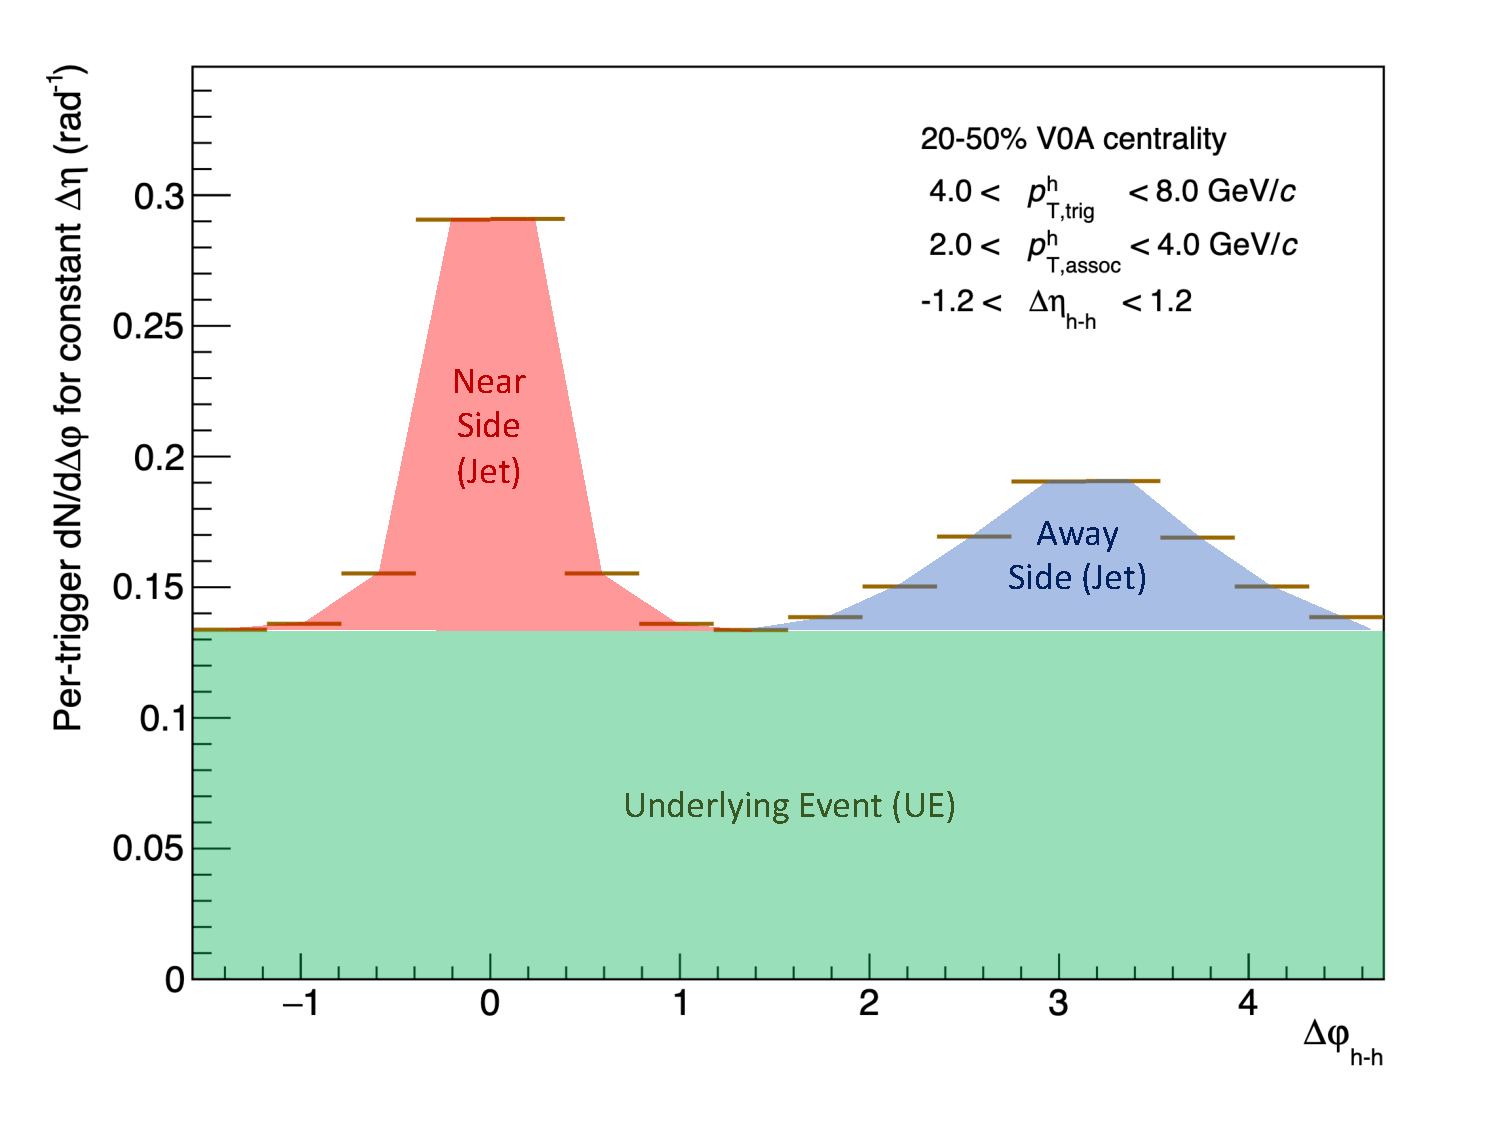
\includegraphics[width=4in]{figures/dphi_regions.pdf}
\caption{A h-h $\Delta\varphi$ distribution taken from this analysis with the near-side, away-side, and uncorrelated regions highlighted.}
\label{dphi_regions}
\end{figure}

For this study, 1-d $\Delta\varphi$ angular correlations of jet-like $h-\Lambda$ and $h-h$ pairs were measured in p-Pb events independently for three multiplicity bins (0-20\%, 20-50\%, 50-80\%), and the final ratios of yields of correlated pairs were compared to study the onset of this enhancement. 


\subsection{Dataset and Event Selection}

\subsubsection{Dataset}

Every event in this analysis was a p-Pb collision at $\sqrt{s_{NN}} =$\SI{5.02}{TeV} taken from the following runlist which consists of 32 runs during the LHC16q period:

\textbf{265525, 265521, 265501, 265500, 265499, 265435, 265427, 265426, 265425, 265424, 265422, 265421, 265420, 265419, 265388, 265387, 265385, 265384, 265383, 265381, 265378, 265377, 265344, 265343, 265342, 265339, 265338, 265336, 265335, 265334, 265332, 265309}


This analysis uses the data from these runs with the FAST reconstruction, corresponding to approximately 400 million minimum bias events.

For the the MC studies (MC method test, MC Closure test), the analysis was performed using the standard purpose generated MC production LHC17f2b\_FAST, anchored to the LHC16q\_FAST production with DPMJET as the generator. This production consists of around 30 million minimum bias events. As more statistics were required to generate a template to correct for the two-track merging effect, the LHC18f3\_FAST and LHC18f3\_CENT\_woSDD productions were used, which are also anchored to LHC16q with DPMJET as the generator. These productions consist of around 400 million minimum bias events (same as our data).

\subsubsection{Event Selection}

Events were selected by requiring a collision Z-vertex of less than \SI{10}{cm} and at least 3 reconstructed tracks in the event.  

This reduces the total number of events (FAST + CENT\_wo\_SDD) considered to approximately 420 million events (see Table \ref{event_table}). The V0A estimator was chosen to determine event multiplicity percentile, and the correlation measurement was performed in three multiplicity percentile bins: \textbf{0-20\%, 20-50\%, and 50-80\%}.

\begin{table}[h!]
    \centering
\begin{tabular}{| c | c | c | c || c | }
\hline
Multiplicity & Total Evts. & Has 3 Tracks & $|Z_{vtx}| <$  10cm + 3 tracks & \% Pass \\
\hline
0-20\% & 1.218E08 & 1.217E08 & 1.061E08 & 87.1\%\\
20-50\% & 1.840E08 & 1.835E08 & 1.590E08 & 86.4\%\\
50-80\% & 1.850E08 & 1.804E08 & 1.563E08 & 84.5\%\\
\hline
\end{tabular}
\caption{Number of events passing our criteria for each multiplicity bin considered.}
\label{event_table}
\end{table}

For all events, the standard Physics selection with pile-up cuts was applied with \texttt{AddTaskPhysicsSelection(kFALSE, kTRUE)}.

\subsection{Code Locations}
The code for this analysis can be found in the following locations:

\textit{Correlations in Data and MC}:
\begin{itemize}
\item  PWGCF/Correlations/DPhi/AliAnalysisTaskLambdaHadronRatio (for $\Lambda$s reconstructed using V0 finder)
\item  PWGLF/Strangeness/DPhi/AliAnalysisTaskLambdaHadronRatioRes (for $\Lambda$s reconstructed using resonance technique) (TBD)
\end{itemize}

\textit{Efficiency Computation}:
\begin{itemize}
\item  PWGLF/Strangeness/DPhi/AliAnalysisTaskLambdaHadronEfficiency (for $\Lambda$s reconstructed using V0 finder and resonance technique) (TBD)
\end{itemize}

\textit{MonteCarlo Closure Test}
\begin{itemize}
\item  PWGLF/Strangeness/DPhi/AliAnalysisTaskLambdaHadronV0Closure (for $\Lambda$s reconstructed using V0 finder) (TBD)
\item  PWGLF/Strangeness/DPhi/AliAnalysisTaskLambdaHadronResClosure (for $\Lambda$s reconstructed using resonance technique) (TBD)
\end{itemize}

\textit{Offline Code}
All of the offline analysis (as well as the code listed above) can be found in my personal github repository at \url{https://github.com/rhanniga}. I take no responsibility for profanity in the commit messages.

\subsection{Relevant Contributions to ALICE Meetings}
This analysis was presented at the following ALICE meetings, in reverse chronological order:

\begin{itemize}
\item Correlations PAG Meeting: 16 May 2023 (\url{https://indico.cern.ch/event/1286625})
\item Correlations PAG Meeting: 9 May 2023 (\url{https://indico.cern.ch/event/1284309})
\item Physics Forum HP2023 Approvals: 13 March 2023 (\url{https://indico.cern.ch/event/1263018})
\item PWG-CF HP2023 Approvals: 6 March 2023 (\url{https://indico.cern.ch/event/1259940})
\item Physics Forum HP2023 Previews: 20 February 2023 (\url{https://indico.cern.ch/event/1253172})
\item PWG-CF HP2023 Previews: 16 February 2023 (\url{https://indico.cern.ch/event/1252451})
\item Strangeness PAG Meeting: 7 February 2023 (\url{https://indico.cern.ch/event/1251426/})
\item Strangeness PAG Meeting: 10 January 2023 (\url{https://indico.cern.ch/event/1237832})
\item Strangeness PAG Meeting: 18 October 2022 (\url{https://indico.cern.ch/event/1211594})
\item Correlations PAG Meeting: 11 October 2022 (\url{https://indico.cern.ch/event/1210412})
\item Strangeness PAG Meeting: 4 October 2022 (\url{https://indico.cern.ch/event/1206673})
\item Resonance PAG Meeting: 17 November 2021 (\url{https://indico.cern.ch/event/1096156})
\item Strangeness PAG Meeting: 4 August 2020 (\url{https://indico.cern.ch/event/943026})
\item Correlations PAG Meeting: 26 June 2020 (\url{https://indico.cern.ch/event/903613})
\item Resonance PAG Meeting: 24 June 2020 (\url{https://indico.cern.ch/event/931429})
\end{itemize}

\section{Track Selection}

\subsection{Associated Hadron Track Cuts}
\label{assoccuts}
For all associated hadrons, a minimum $p_{T}$ cuts of $p_{T} >$ \SI{0.15}{GeV/c} was applied.  Additinally, an $\eta$ cut of $|{\eta}| < 0.8$ was required. Furthermore, all associated hadrons were required to meet the standard cuts supplied by \texttt{AliESDtrackCuts::GetStandardITSTPCTrackCuts2011()} corresponding to track filter bit 1024, with a modified number of MinNClustersTPC from the standard cut of 50:

\begin{itemize}
    \item TPC Refit
    \item ITS Refit
	\item \textbf{SetMinNClustersTPC: 80}
	\item SetMaxChi2PerClusterTPC: 4
	\item SetAcceptKinkDaughters: kFALSE
	\item SetMaxDCAToVertexZ: 2
	\item SetMaxDCAToVertexXYPtDep: $0.0105+0.0350/p_{T}^{1.1}$
	\item SetDCAToVertex2D: kFALSE
	\item SetMaxChi2TPCConstrainedGlobal: 36
	\item SetRequireSigmaToVertex: kFALSE
	\item SetMaxChi2PerClusterITS: 36
\end{itemize}

For the correlation, the associated hadron is selected only in the momentum region

$${1.0 < p_{T} < \SI{4.0}{GeV/c}},$$ 

with further binning performed offline. The $\it{p}_{T}$, $\varphi$ and $\eta$ distributions for the associated hadrons that pass these cuts in the 0-20\% multiplicity bin can be seen in Figure \ref{assoc_plots}.

\begin{figure}[ht]
\centering
\begin{subfigure}{
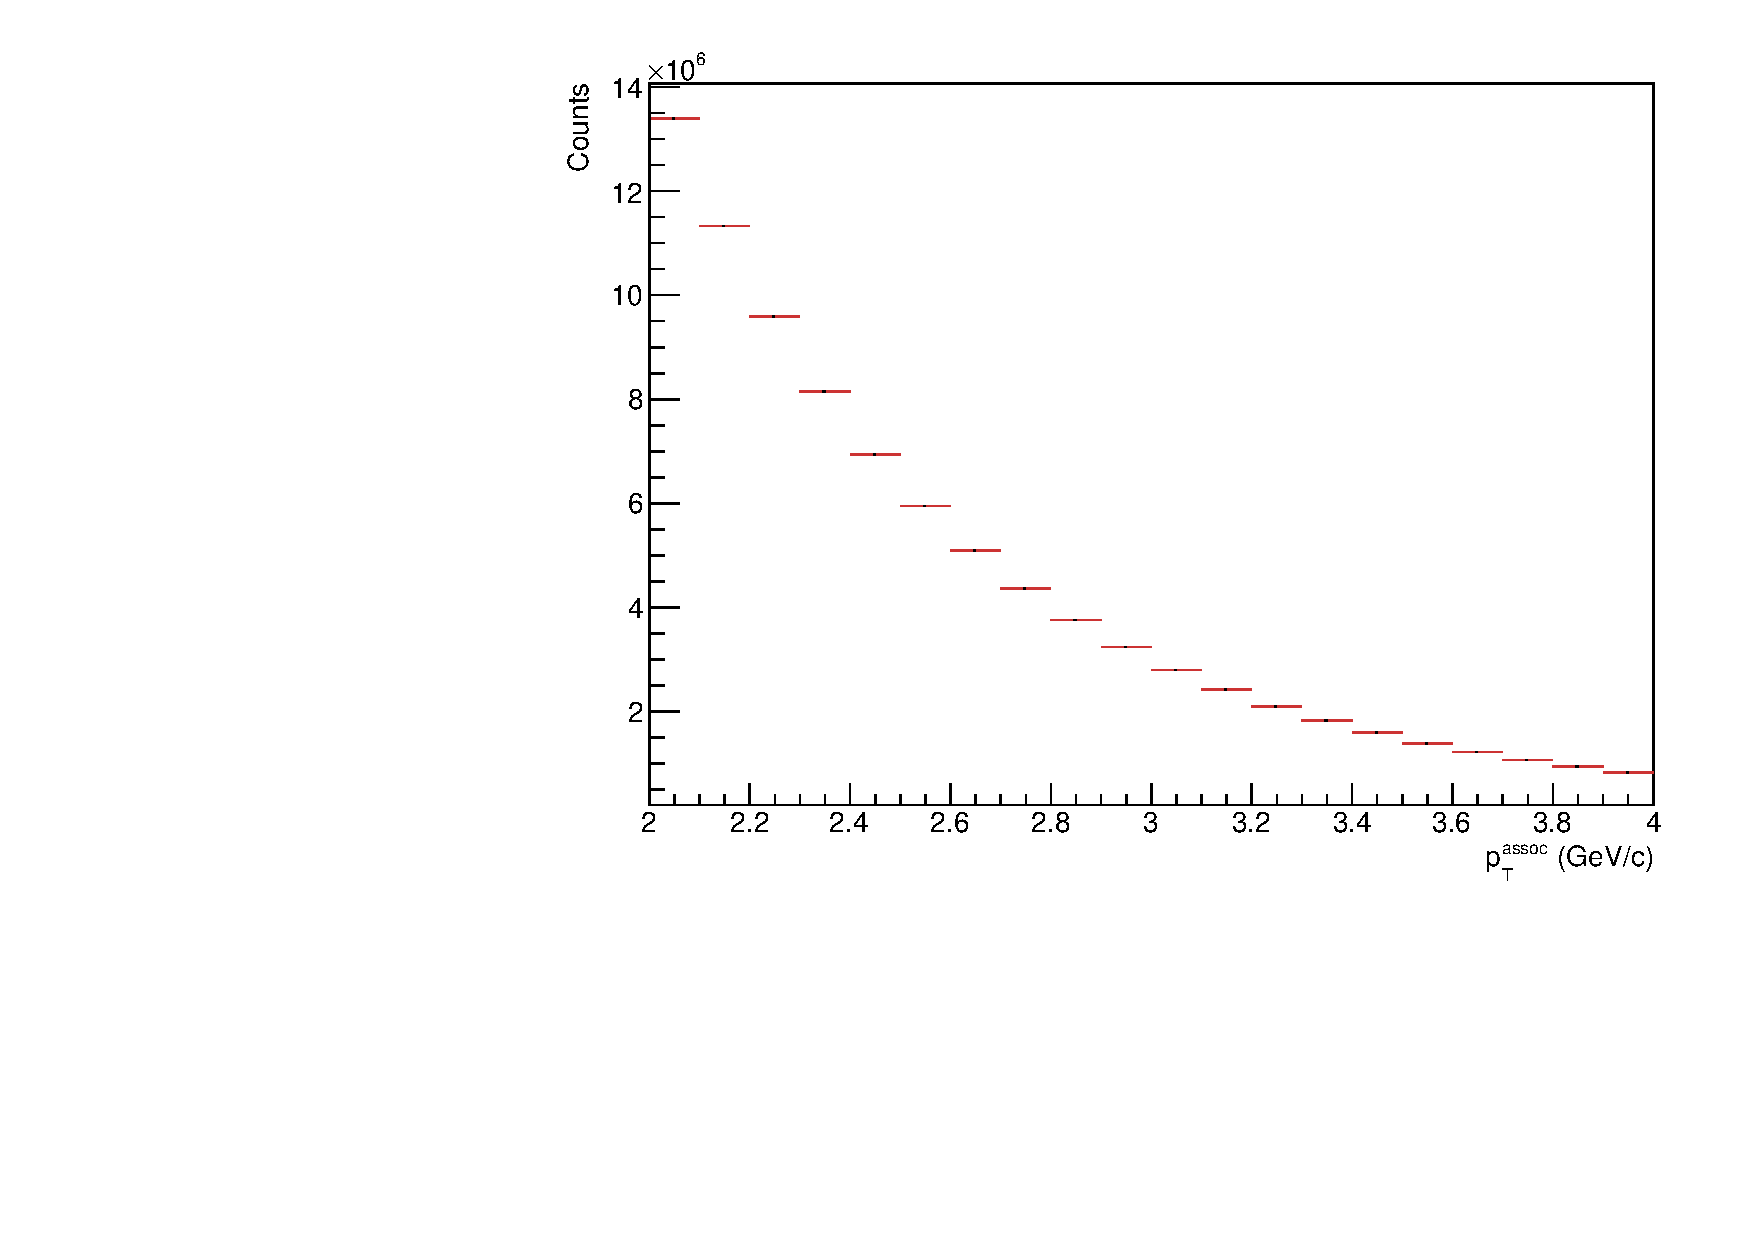
\includegraphics[width=4in]{figures/assoc_pt_dist_0_20.pdf}}
\end{subfigure}
\begin{subfigure}{
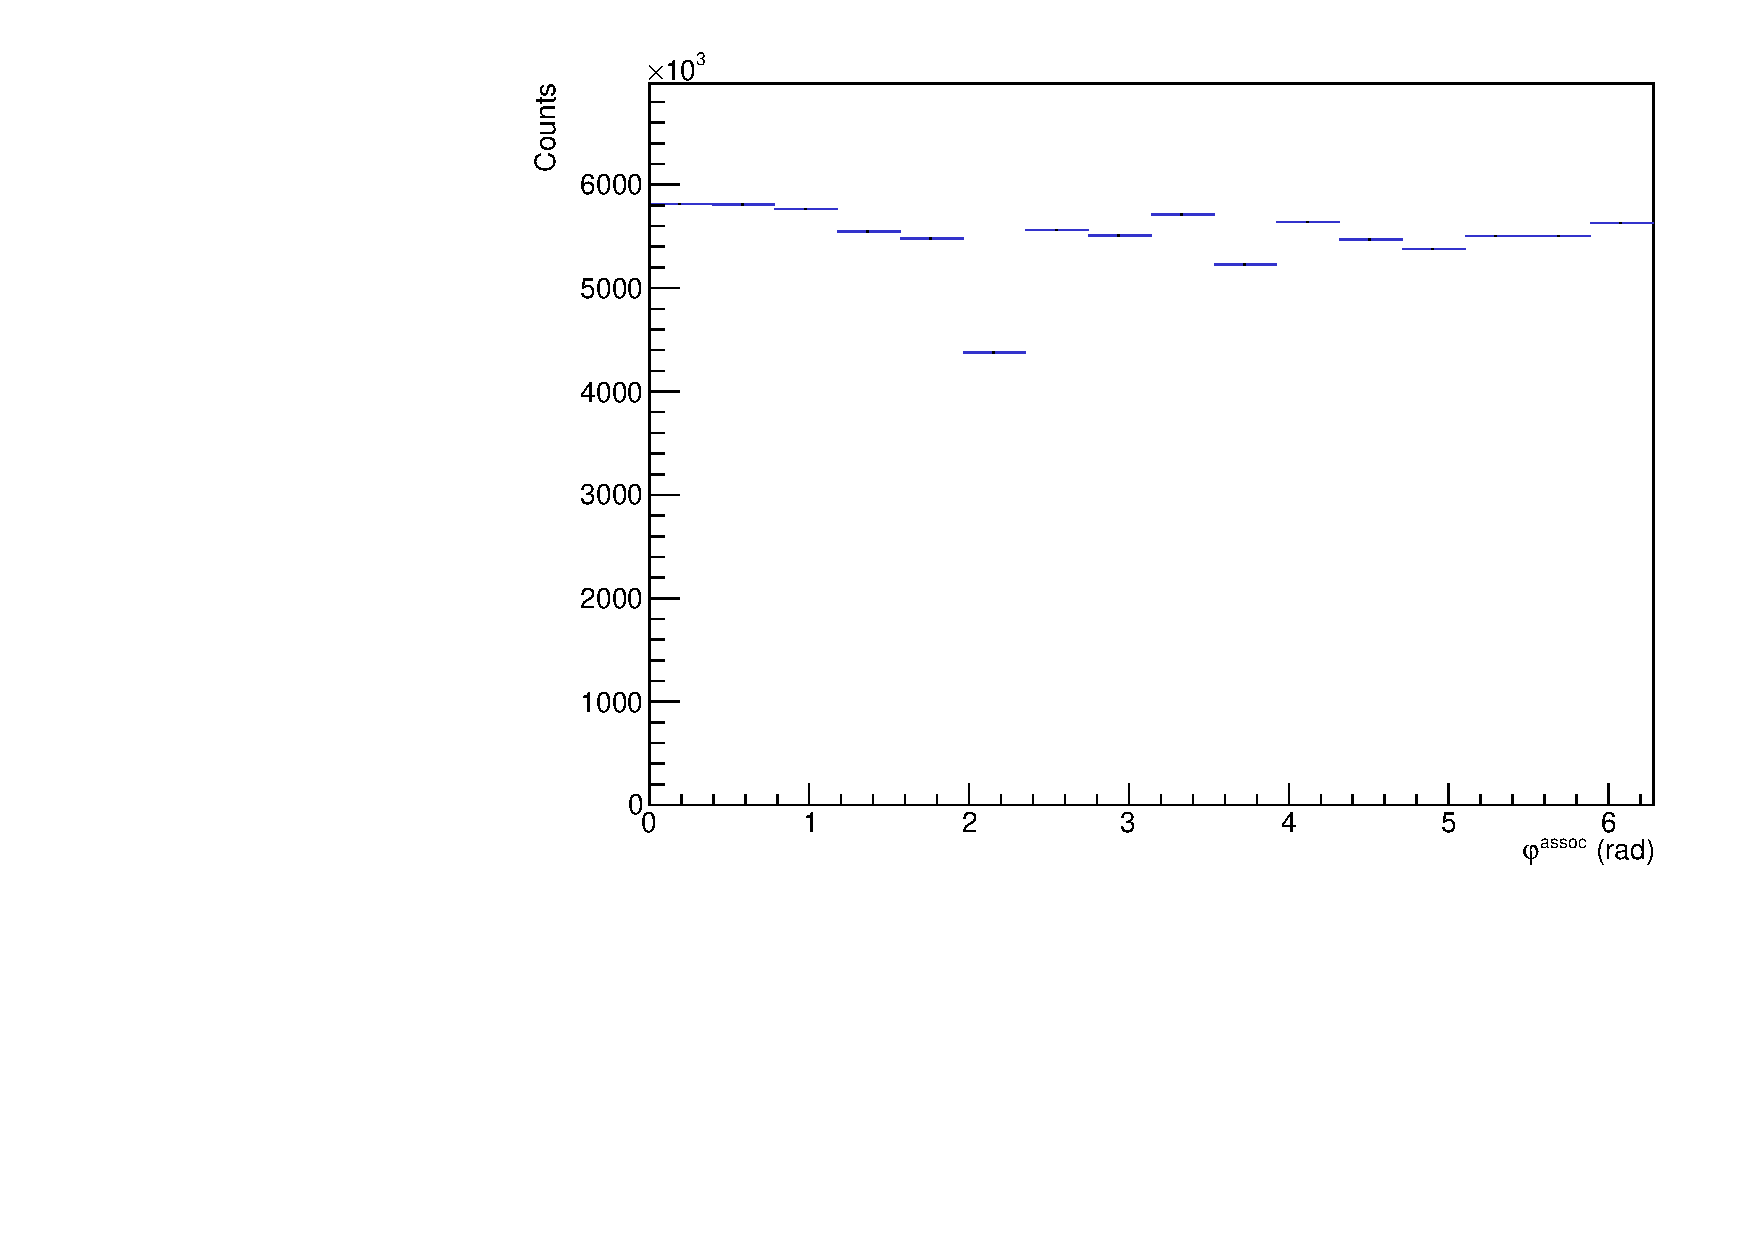
\includegraphics[width=4in]{figures/assoc_phi_dist_0_20.pdf}}
\end{subfigure}
\begin{subfigure}{
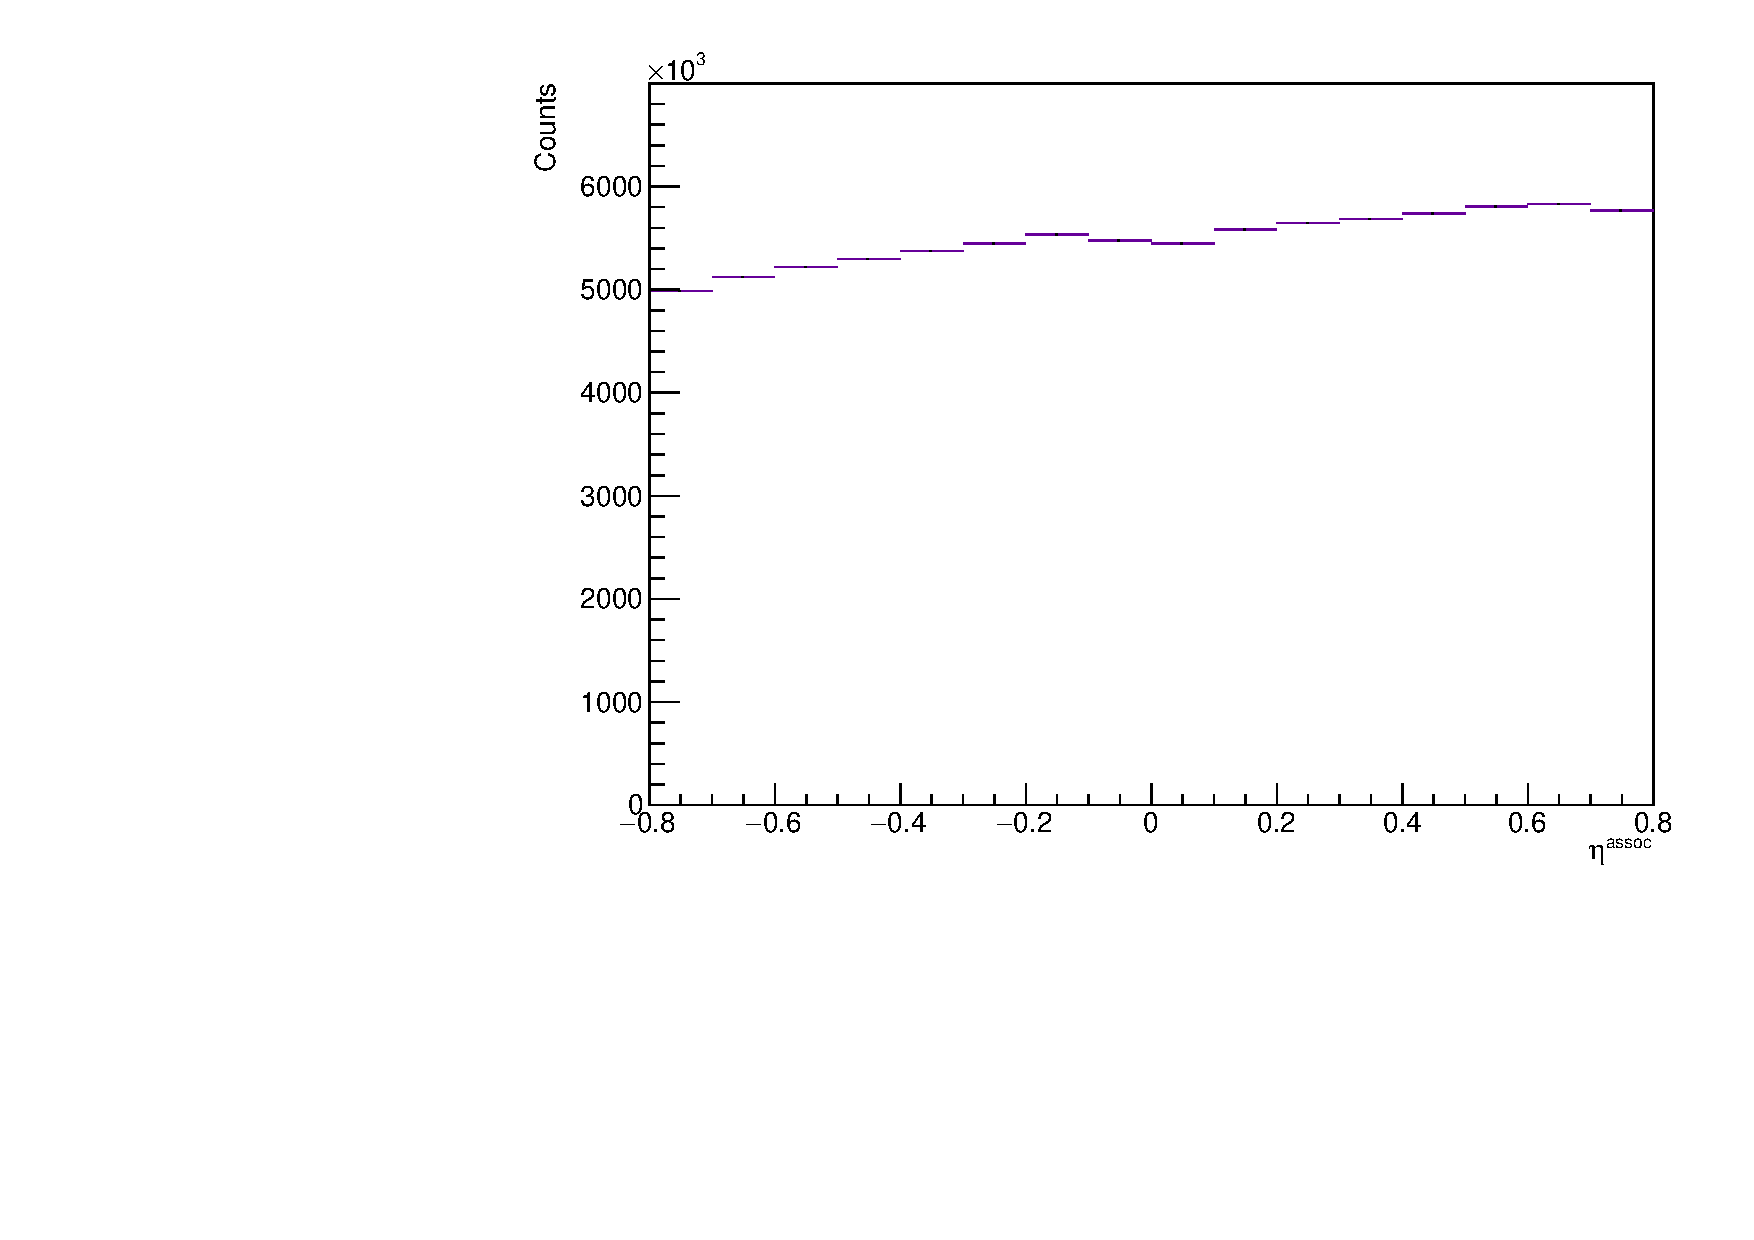
\includegraphics[width=4in]{figures/assoc_eta_dist_0_20.pdf}}
\end{subfigure}
\caption{The $\it{p}_{T}$ (top), $\varphi$ (center) and $\eta$ (bottom) distributions for the associated hadrons in the multiplicity range 0-20\%.}
\label{assoc_plots}
\end{figure}



\subsection{$\Lambda$ Daughter Proton and Pion Track Cuts}
\label{daughtercuts}
The proton and the pion are required to have a minimum $p_{T}$ of $p_{T} >$ \SI{0.15}{GeV/c} and an $\eta$ cut of $|{\eta}| < 0.8$. Furthermore, the proton and pion are required to meet the following quality cuts:
\begin{itemize}
	\item TPC refit flag enabled
	\item TPC crossed rows $>$ 70
	\item (TPC crossed rows)/(findable clusters) $>$ 0.8
\end{itemize}
All of these cuts are applied to the daughters of the reconstructed $\Lambda$, independent of the technique used for said reconstruction. For the correlation, the reconstructed $\Lambda$ is selected only in the momentum region

$${1.0 < p_{T} < \SI{4.0}{GeV/c}},$$

with further binning performed offline.

\subsection{Trigger Track Cuts}
\label{trigcuts}
For the trigger hadron tracks, Hybrid Global constrained tracks were accepted using the cuts supplied by \texttt{IsHybridGlobalConstrainedGlobal()}, or track bit 20, or BIT(20), or 1048576, or filter mask 768:

\begin{itemize}
	\item SetMinNClustersTPC: 50
	\item SetMaxChi2PerClusterTPC: 4
	\item SetAcceptKinkDaughters: kFALSE
	\item SetMaxDCAToVertexZ: 3.2
	\item SetMaxDCAToVertexXY: 2.4
	\item SetDCAToVertex2D: kTRUE
	\item SetMaxChi2TPCConstrainedGlobal(36)
	\item SetMaxFractionSharedTPCClusters(0.4)
\end{itemize}

For the both the di-hadron and h-$\Lambda$ correlation, the trigger hadron is selected in the momentum region:

$${4.0 < p_{T} < \SI{8.0}{GeV/c}}.$$

The $\it{p}_{T}$, $\varphi$ and $\eta$ distributions for the trigger hadrons that pass these cuts in the 0-20\% multiplicity bin can be seen in Figure \ref{trig_plots}.

\begin{figure}[ht]
\centering
\begin{subfigure}{
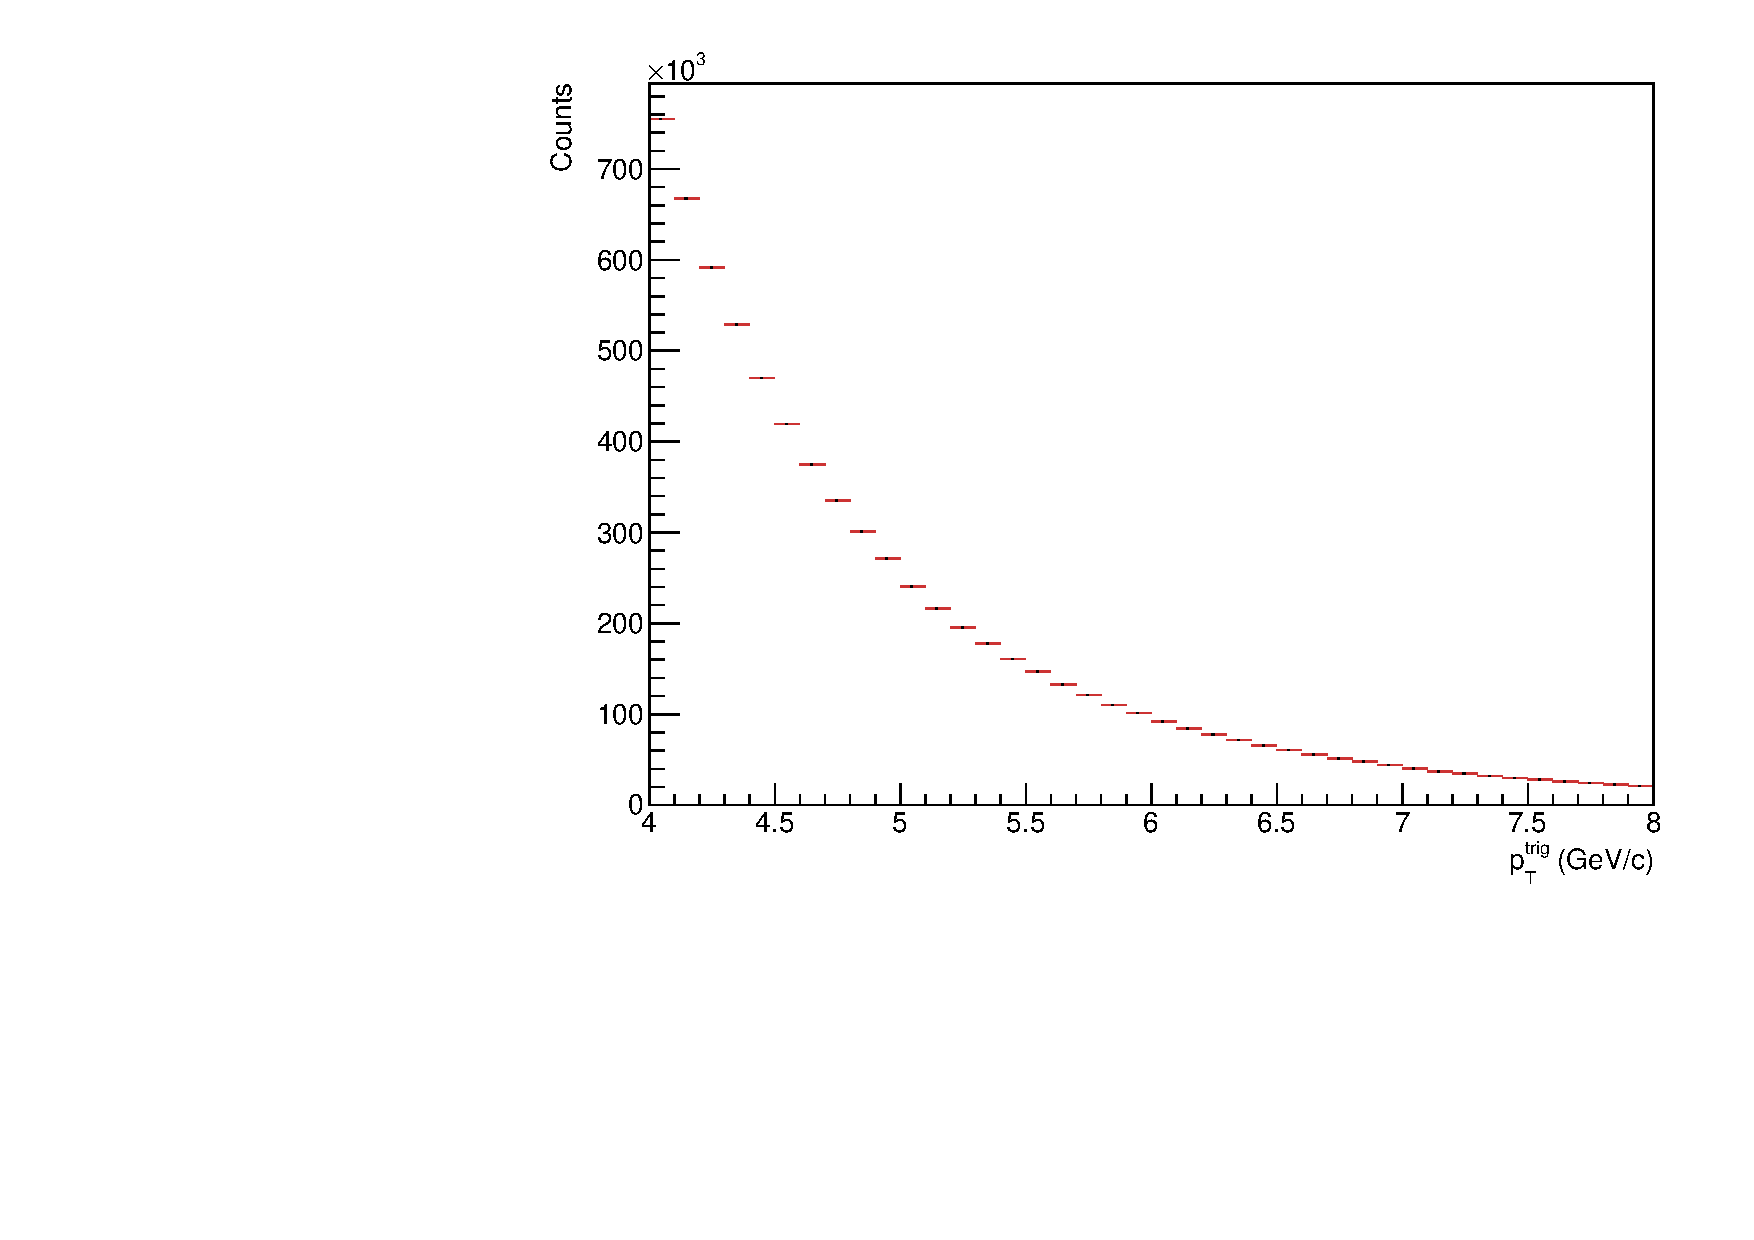
\includegraphics[width=4in]{figures/trig_pt_dist_0_20.pdf}}
\end{subfigure}
\begin{subfigure}{
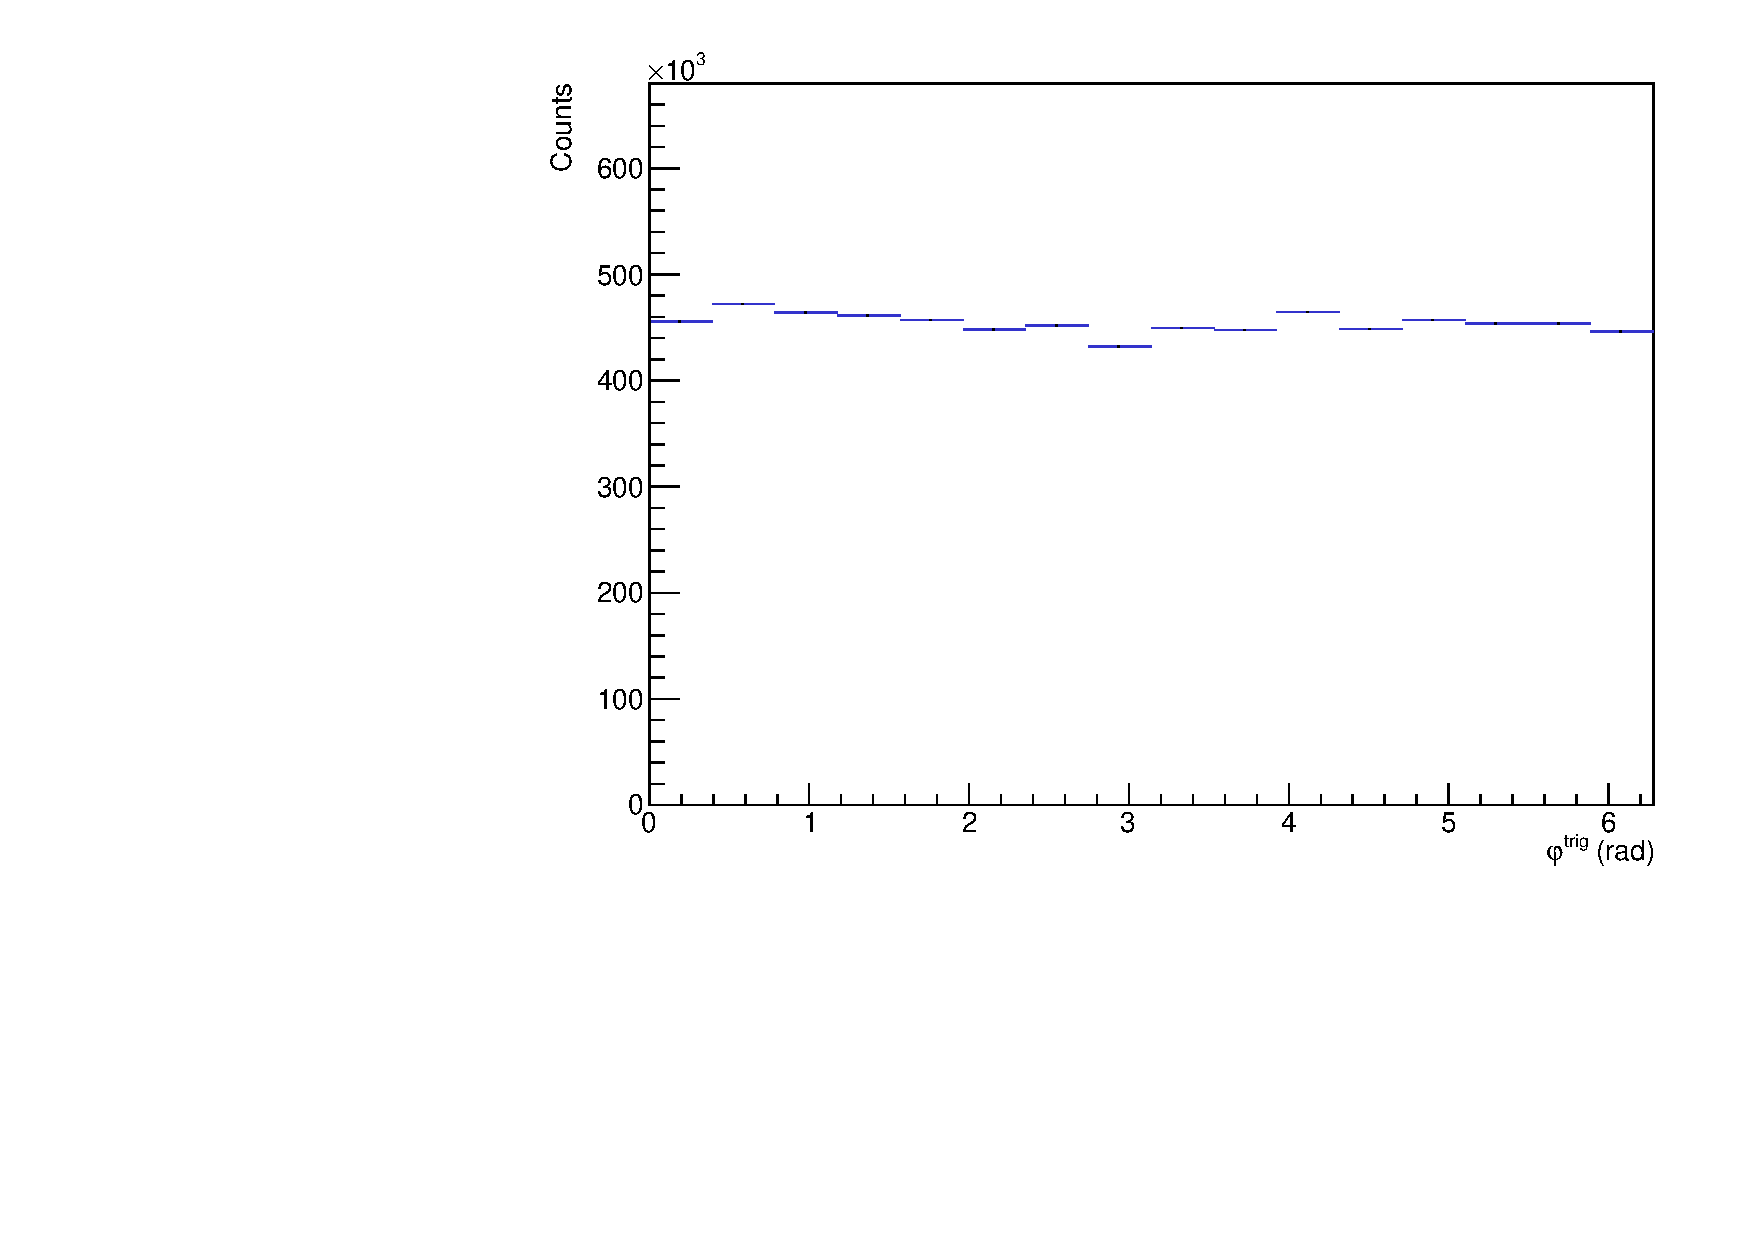
\includegraphics[width=4in]{figures/trig_phi_dist_0_20.pdf}}
\end{subfigure}
\begin{subfigure}{
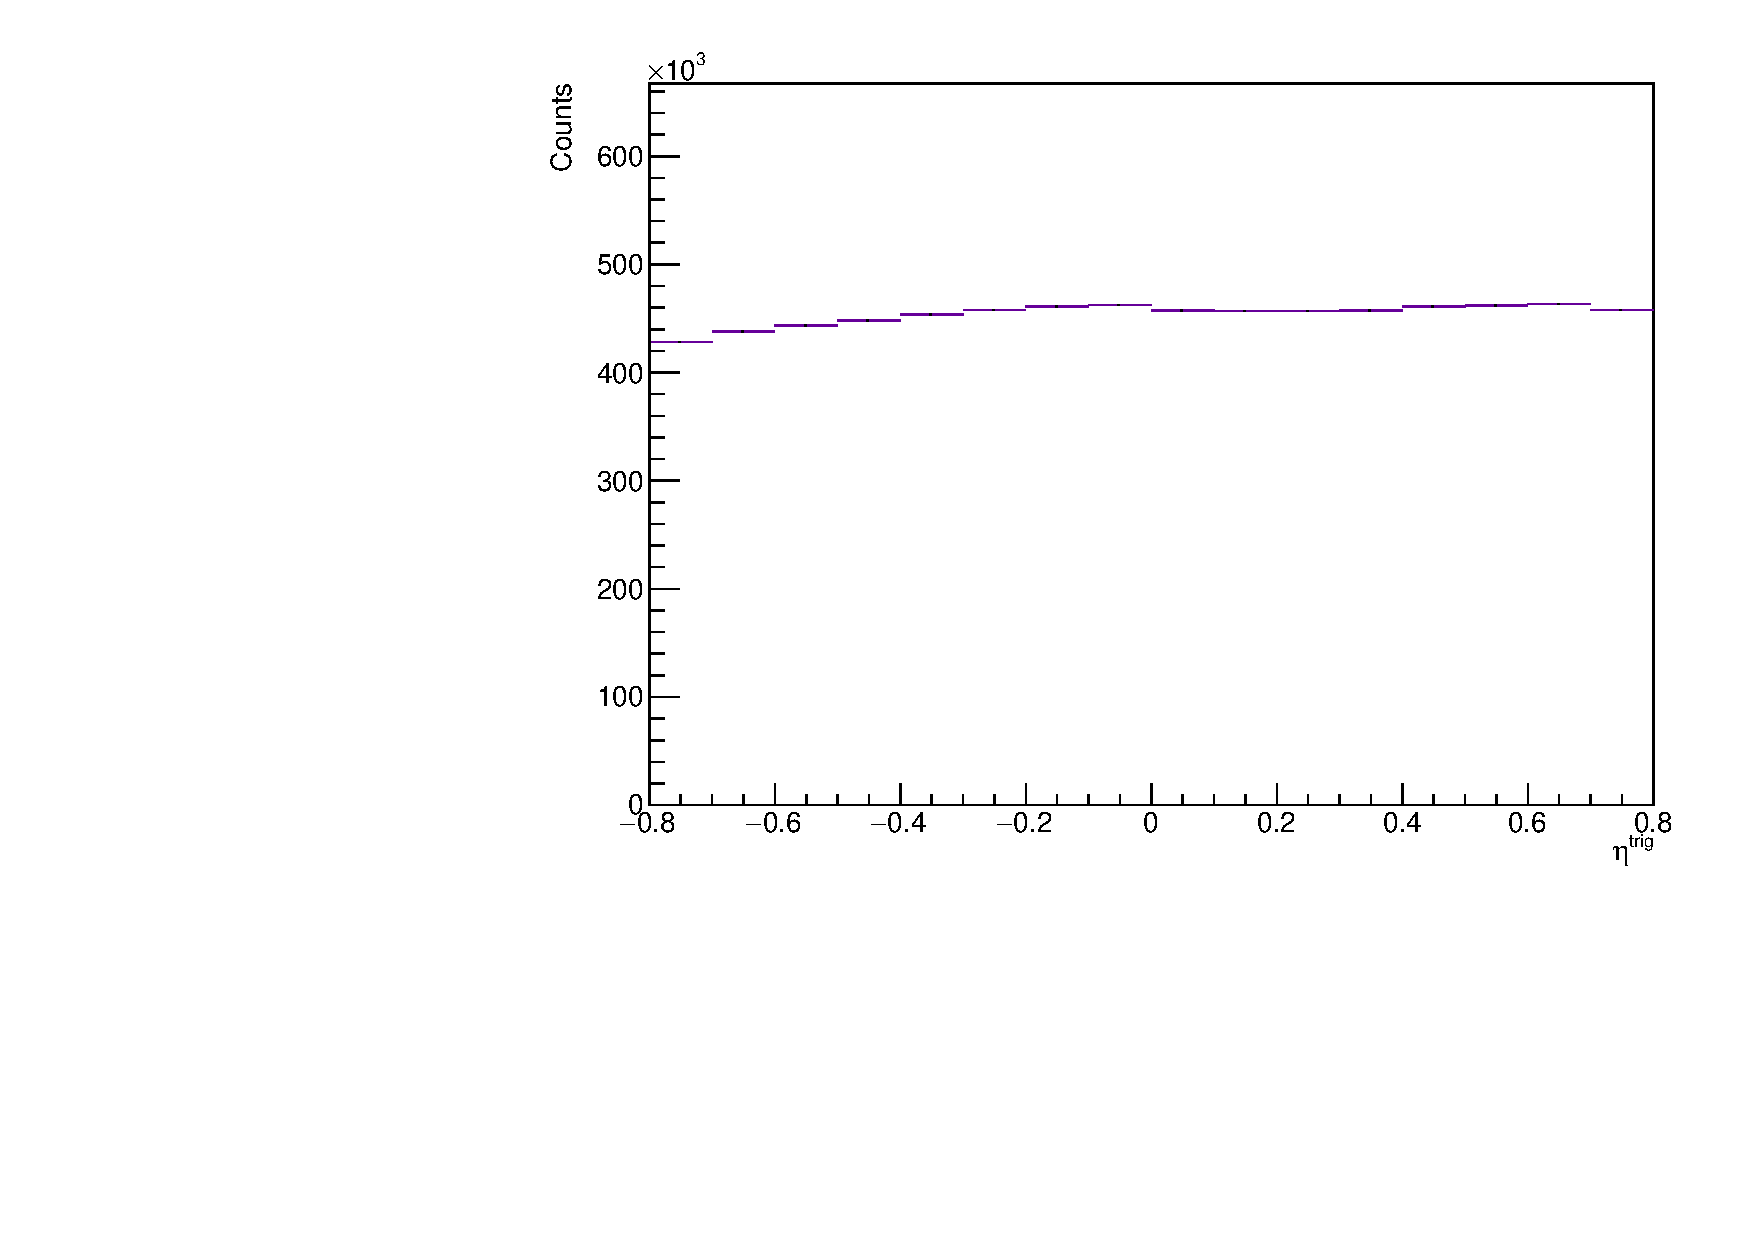
\includegraphics[width=4in]{figures/trig_eta_dist_0_20.pdf}}
\end{subfigure}
\caption{The $\it{p}_{T}$ (top), $\varphi$ (center) and $\eta$ (bottom) distributions for the trigger hadrons in the multiplicity range 0-20\%. Note that the $\varphi$ and $\eta$ distributions are uniform, indicating no geometric biases from track selection (TPC sector bounds, etc.) will be introduced into the angular correlations.}
\label{trig_plots}
\end{figure}

\clearpage

\section{$\Lambda$ Reconstruction}
\label{lambda_reconstruction}

The $\Lambda$ candidates were reconstructed through the $\Lambda \rightarrow p\pi^{-}$ ($\bar{\Lambda} \rightarrow \pi^{+}p$) decay channel with a branching ratio of 63.9\%. For the majority of this analysis, the $\Lambda$ and $\bar{\Lambda}$ are combined together. Thus, unless otherwise specified, $\Lambda = \Lambda + \bar{\Lambda}$. 

The $\Lambda$ candidates in this analysis were reconstructed using two separate techniques:
\begin{itemize}
	\item \textbf{V0 Finder Technique} - The V0 finder technique reconstructs the $\Lambda$ by combining the proton and pion tracks with the V0 finder algorithm, which can be found within the AliROOT framework.
	\item \textbf{Resonance Technique} - The resonance technique combines all oppositely charged proton-pion pairs to reconstruct the $\Lambda$, resulting in maximal statistics at the cost of a large combinatorial background.
\end{itemize}

The central points in this analysis are from $\Lambda$ candidates reconstructed using the V0 finder technique. The resonance technique serves as a powerful cross-check to ensure no topological biases are introduced within the V0 finder algorithm, and is investigated in detail in Section \ref{resonance_technique}.

\subsection{V0 Selection}
\label{v0_selection}
The central points in this analysis were generated using $\Lambda$s reconstructed using the V0-finder algorithm found within the AliROOT framework. All of the V0s found by the V0 finder algorithm were required to pass the following cuts:

\begin{itemize}
	\item $p_{T} > 0.2$ GeV/$c$
	\item $|\eta| < 0.8$
	\item On the fly status: disabled (offline V0s only)
\end{itemize}

There were no additional topological cuts applied to the V0s or their corresponding daughters. This was done to maximize statistics and to minimize any topological biases beyond those introduced by reconstructing $\Lambda$s using the V0-finder algorithm.

\subsection{V0 Daughter PID Cuts}
\label{v0_daughter_pid}
The daughter protons and pions were required to meet the following PID cuts using both the TPC and TOF detectors:

\begin{itemize}
	\item[$\ast$] $|n\sigma_{TPC, p}| < 2$
	\item[$\ast$] $|n\sigma_{TPC, \pi}| < 3$
	\item[$\ast$] $|n\sigma_{TOF, p}| < 2$ (if signal exists)
	\item[$\ast$] $|n\sigma_{TOF, \pi}| < 3$ (if signal exists)
\end{itemize}

The $n\sigma$ values for both the TPC and TOF detectors of the daughter proton and pion are shown in Figure \ref{nsigma_tpc} and Figure \ref{nsigma_tof}, respectively. These values were obtained from the AOD tracks associated with every V0 found by the V0 finder algorithm, provided that those tracks also pass the aforementioned daughter track quality cuts.

To account for any biases introduced from choosing daughter tracks from the V0 finder algorithm, the TPC and TOF $n\sigma_{p, \pi}$ distributions are shown for all AOD tracks in the tracklist in Figure \ref{nsigmatofvtpc}. There are no major differences between the $n\sigma$ distributions of the daughter tracks from the V0 finder algorithm and the AOD tracks in the tracklist. This indicates that the V0 finder algorithm is not introducing any biases in the PID selection of the daughter tracks. These plots also represent the PID cuts used for the resonance technique, which utilizes the full AOD track list and will be discussed in Section \ref{resonance_technique}.


\begin{figure}[ht]
\centering
\begin{subfigure}{
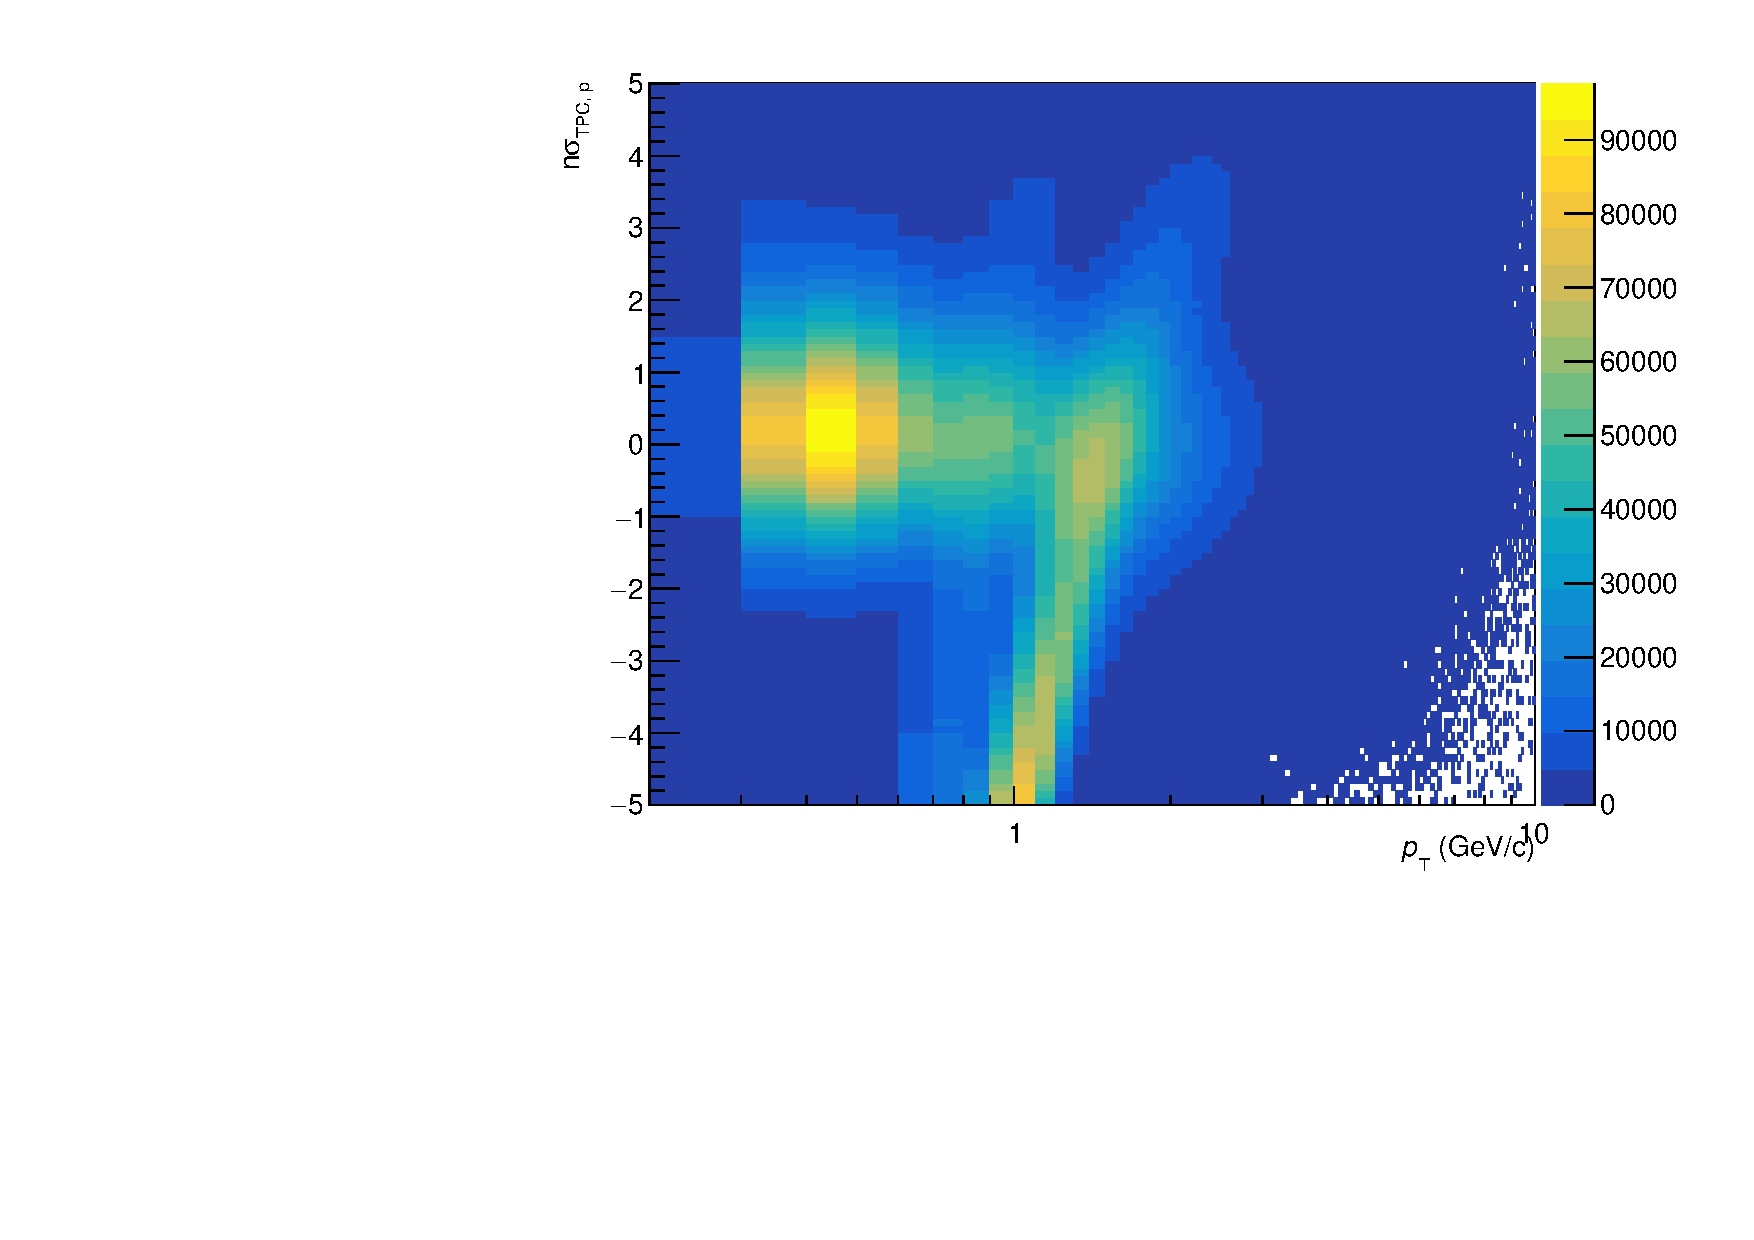
\includegraphics[width=3in]{figures/nsigma_tpc_proton.pdf}}
\end{subfigure}
\begin{subfigure}{
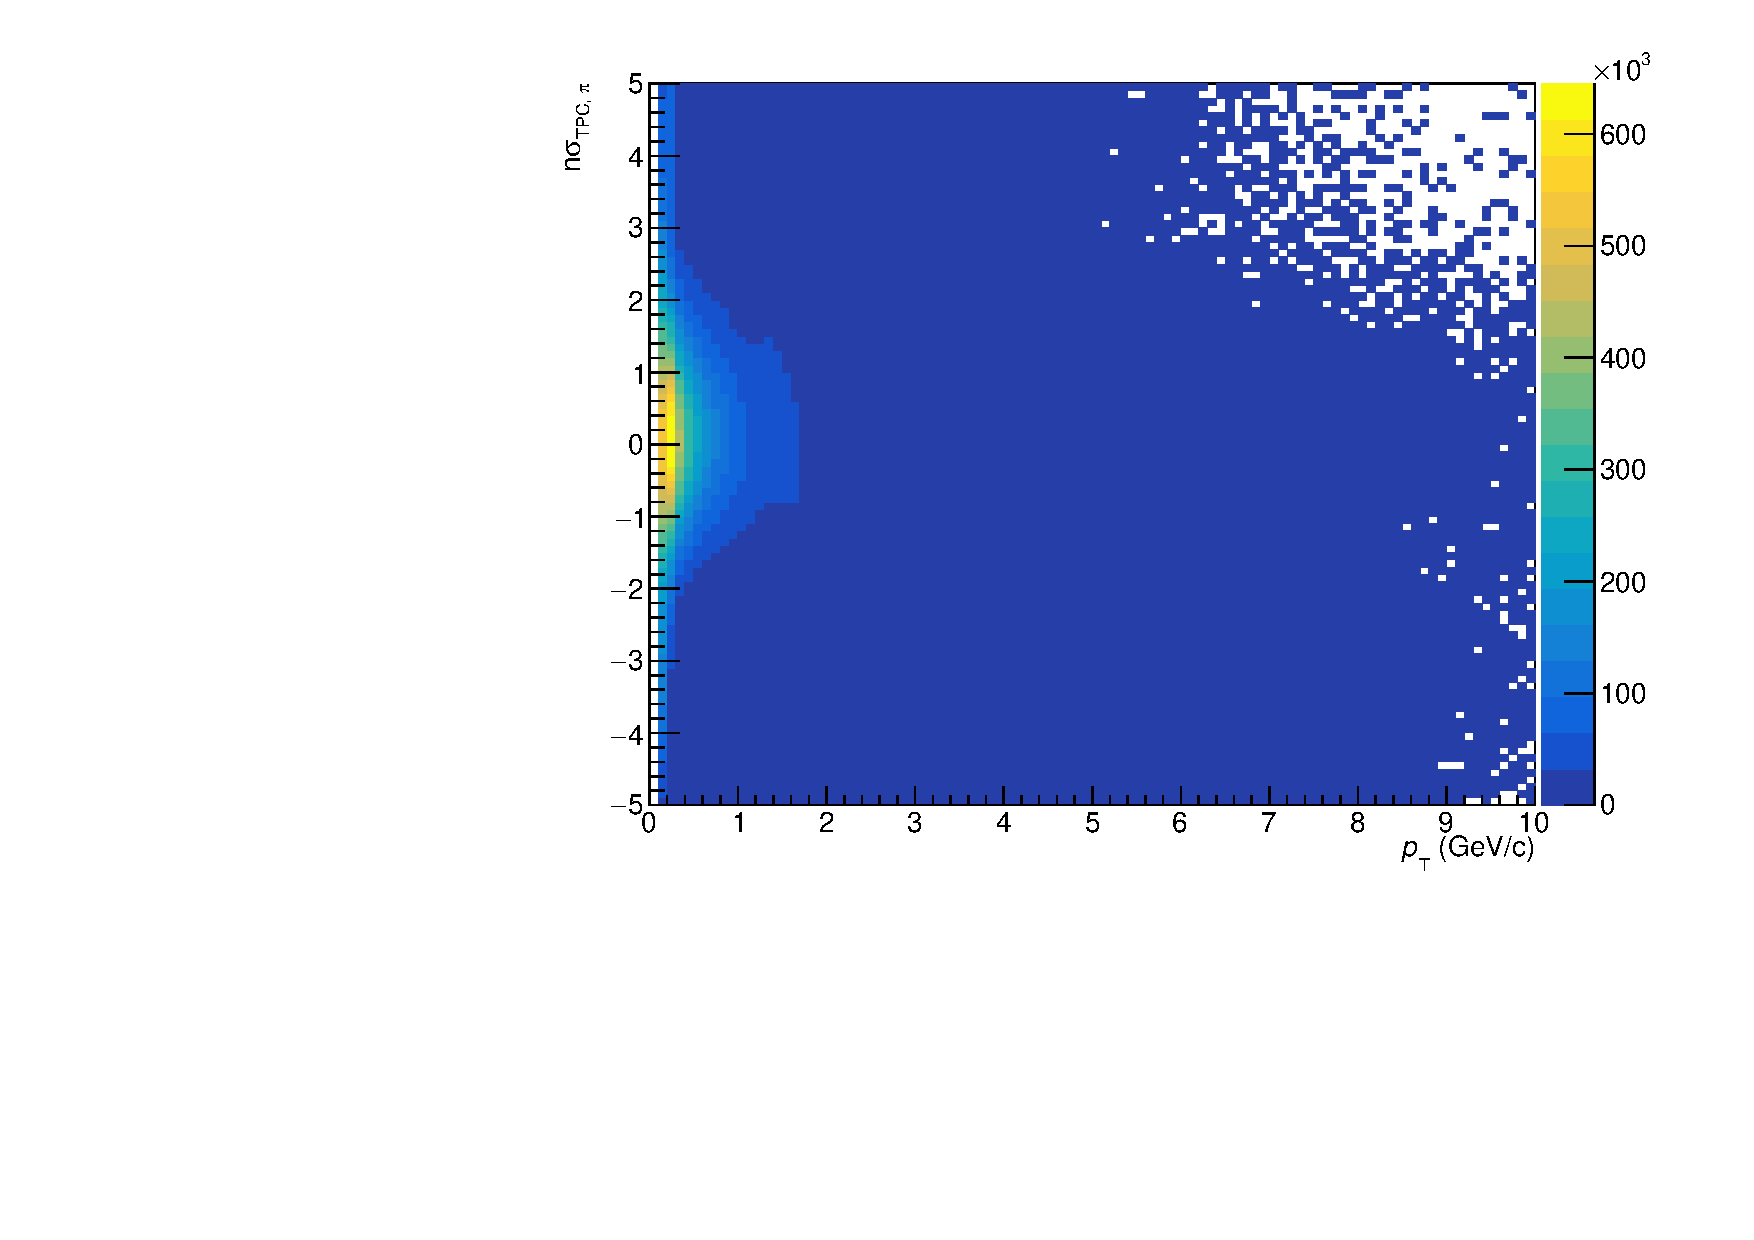
\includegraphics[width=3in]{figures/nsigma_tpc_pion.pdf}}
\end{subfigure}
\caption{$n\sigma$ for protons (left) and pions (right) in the TPC detector as a function of $p_{T}$. A wider PID cut is used for the pion to maximize the $\Lambda$ signal.}
\label{nsigma_tpc}
\end{figure}

\begin{figure}[ht]
\centering
\begin{subfigure}{
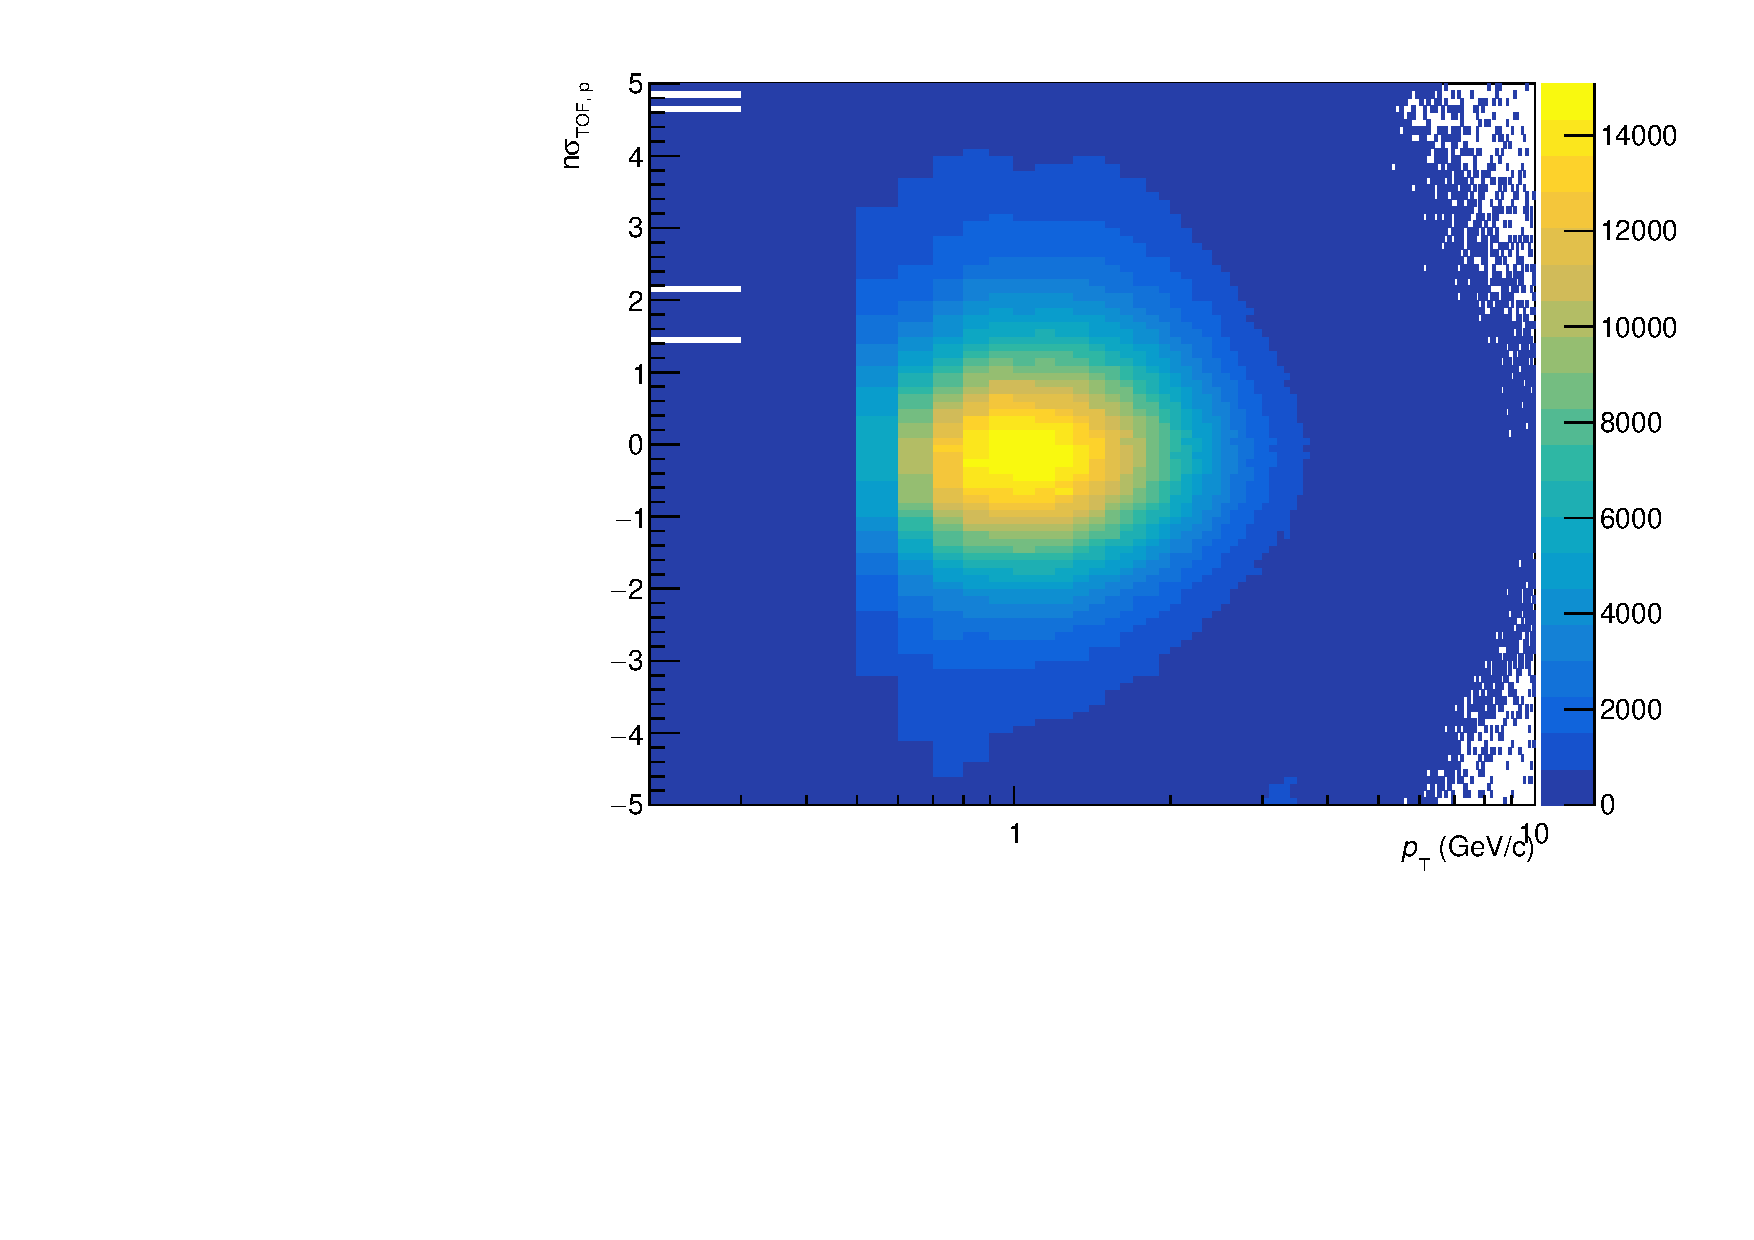
\includegraphics[width=3in]{figures/nsigma_tof_proton.pdf}}
\end{subfigure}
\begin{subfigure}{
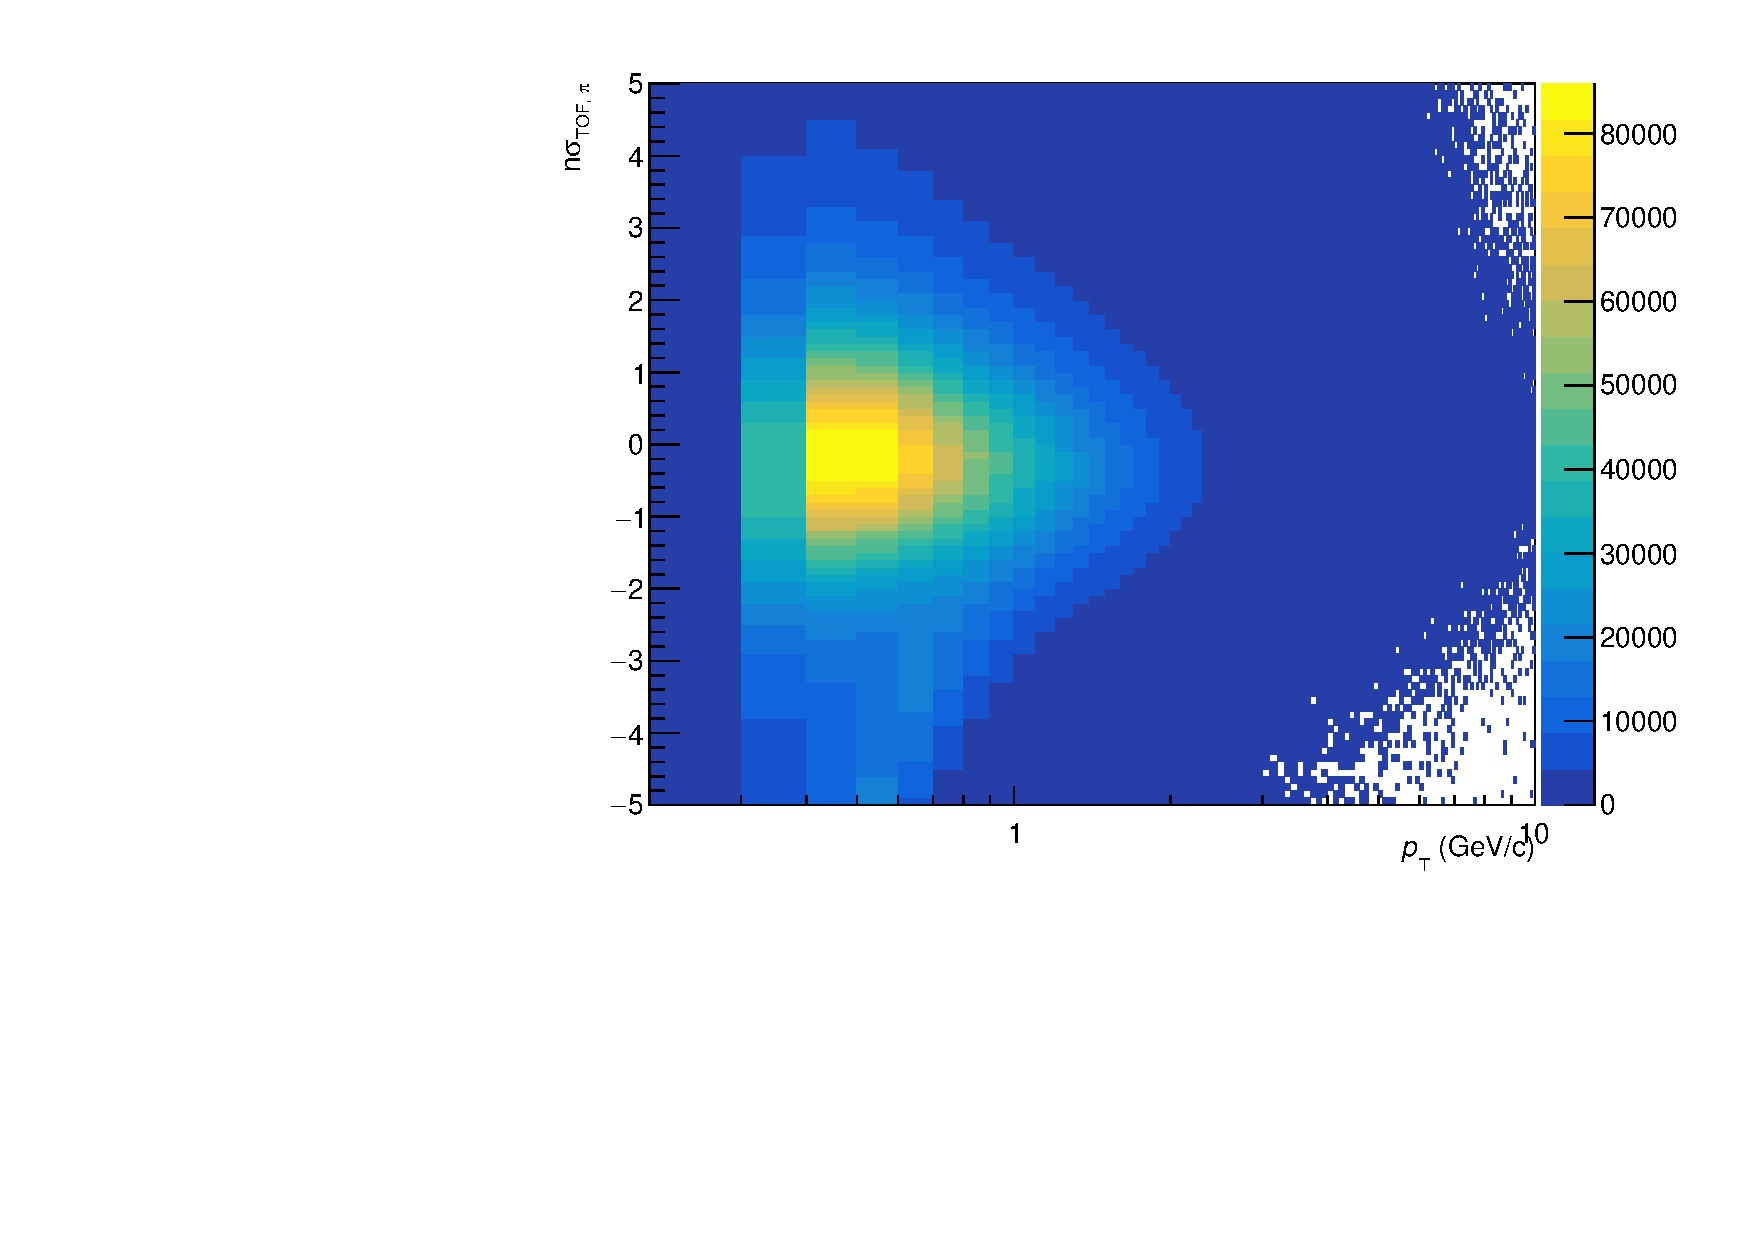
\includegraphics[width=3in]{figures/nsigma_tof_pion.pdf}}
\end{subfigure}
\caption{$n\sigma$ for protons (left) and pions (right) in the TOF detector as a function of $\it{p}_{T}$. If there is no TOF signal for the track, the TOF PID cut is not applied.}
\label{nsigma_tof}
\end{figure}

\begin{figure}[ht]
\centering
\begin{subfigure}{
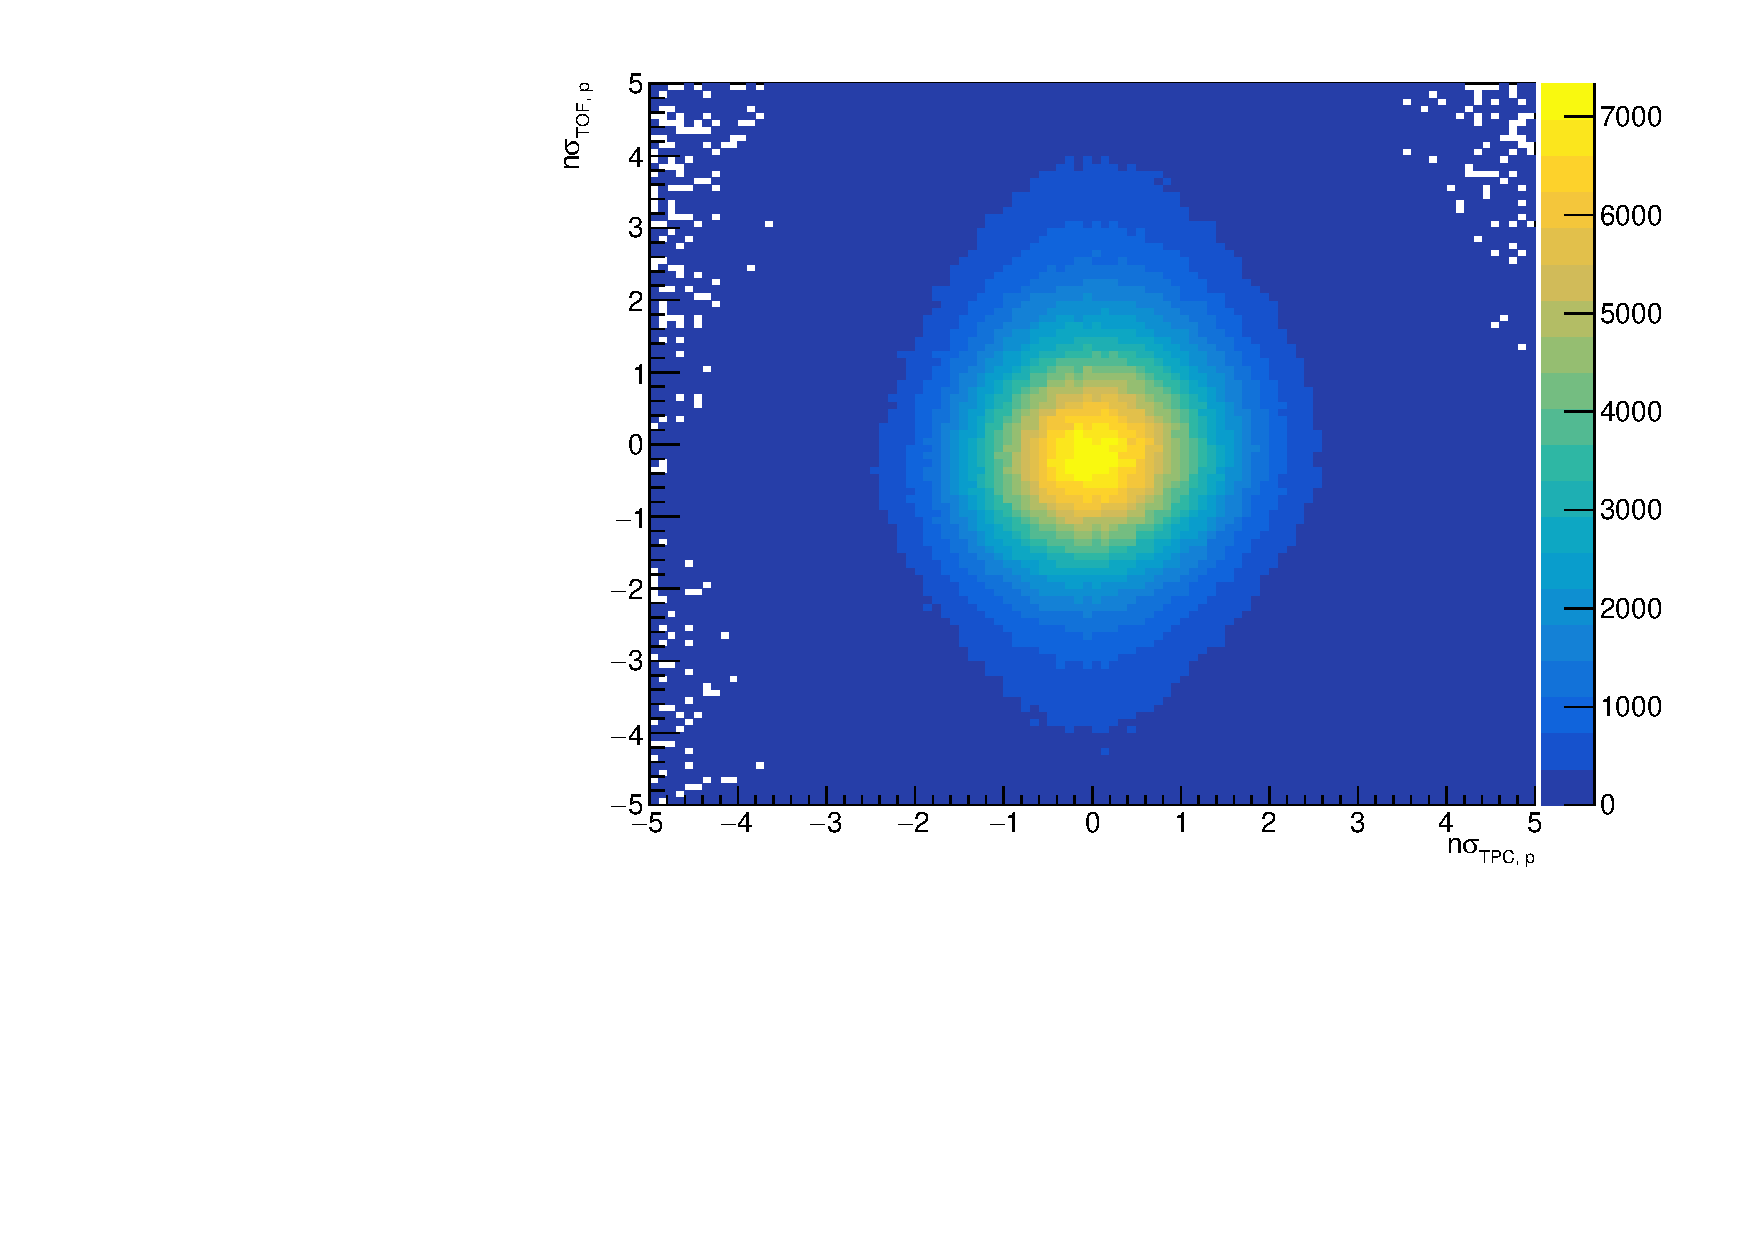
\includegraphics[width=3in]{figures/nsigma_tof_v_tpc_proton.pdf}}
\end{subfigure}
\begin{subfigure}{
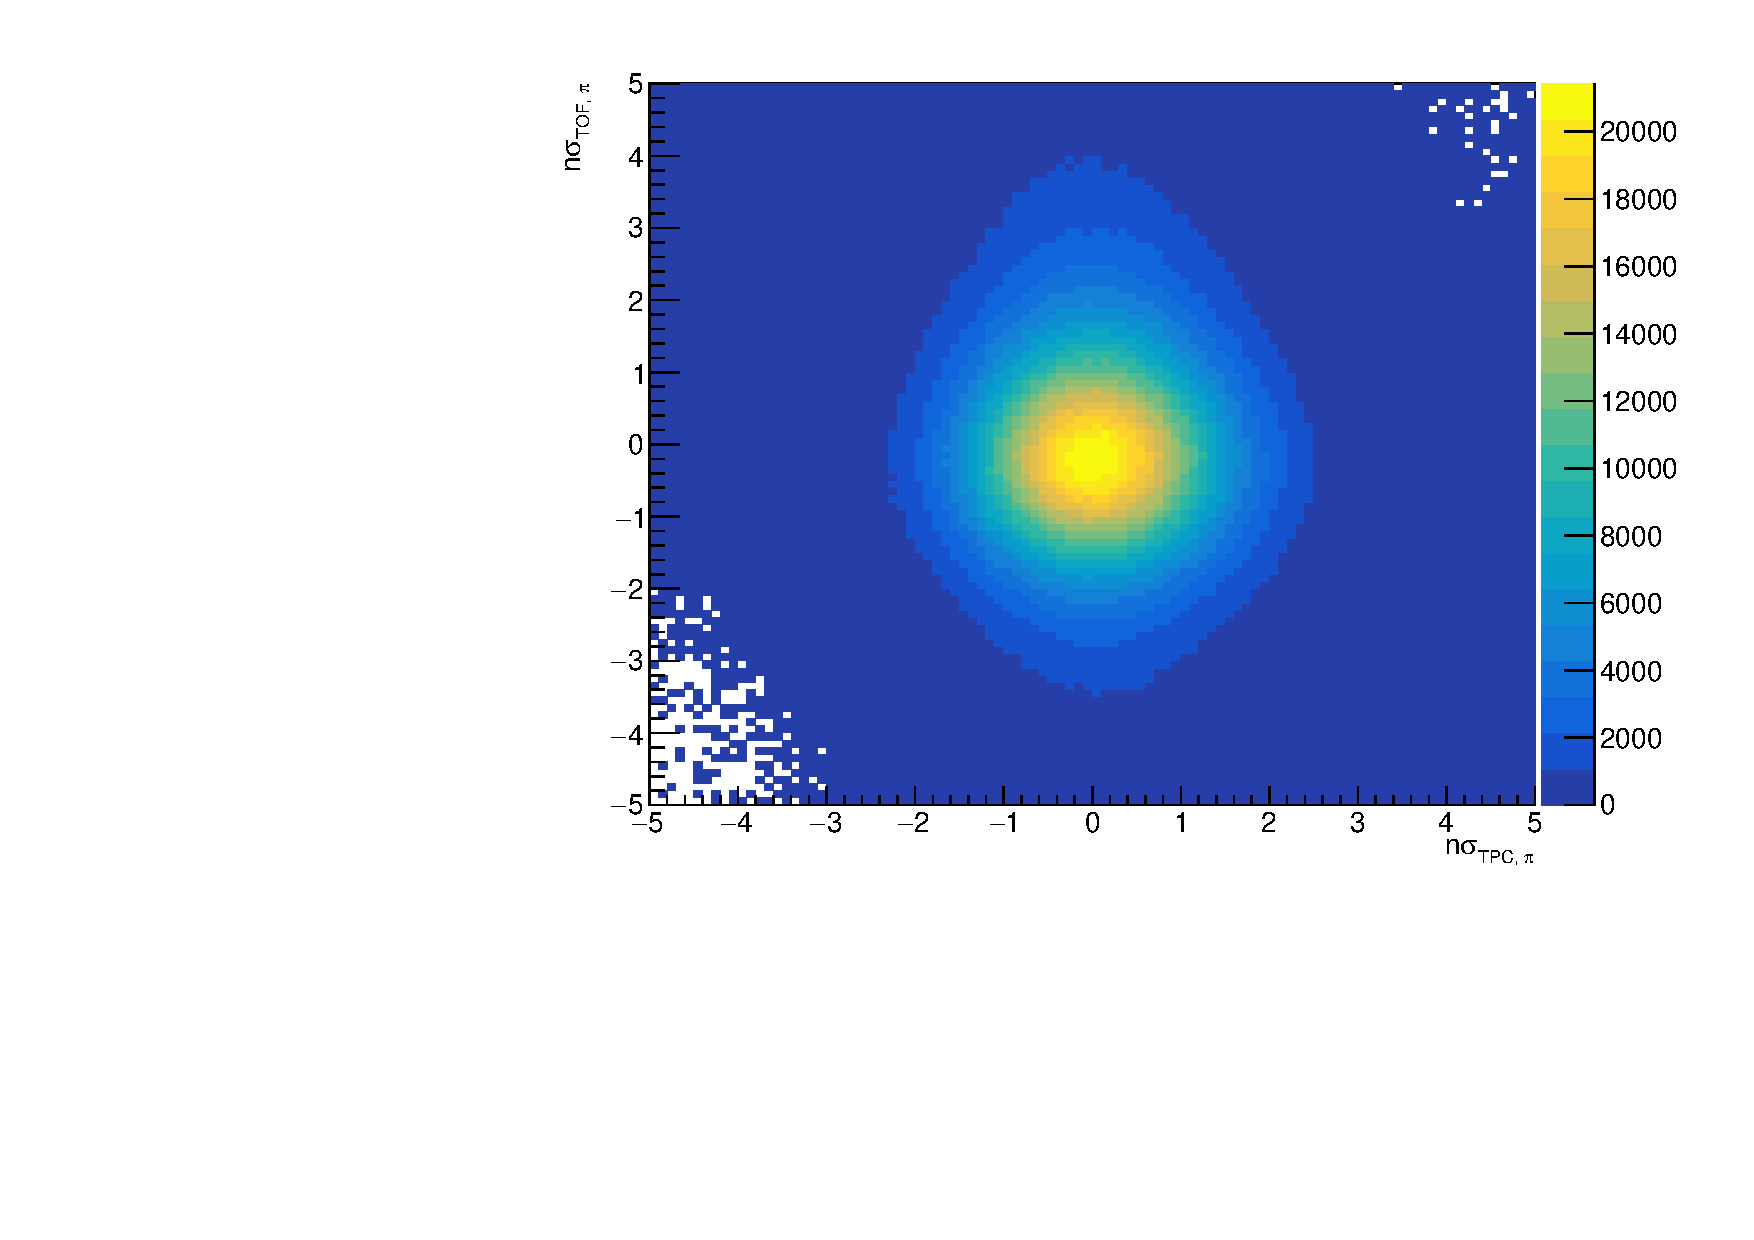
\includegraphics[width=3in]{figures/nsigma_tof_v_tpc_pion.pdf}}
\end{subfigure}
\caption{$n\sigma$ in TOF vs $n\sigma$ in TPC for protons (left) and pions (right). No contimatination is observed for both of the particle species.}
\label{nsigmatofvtpc}
\end{figure}

\begin{figure}[ht]
\centering
\begin{subfigure}{
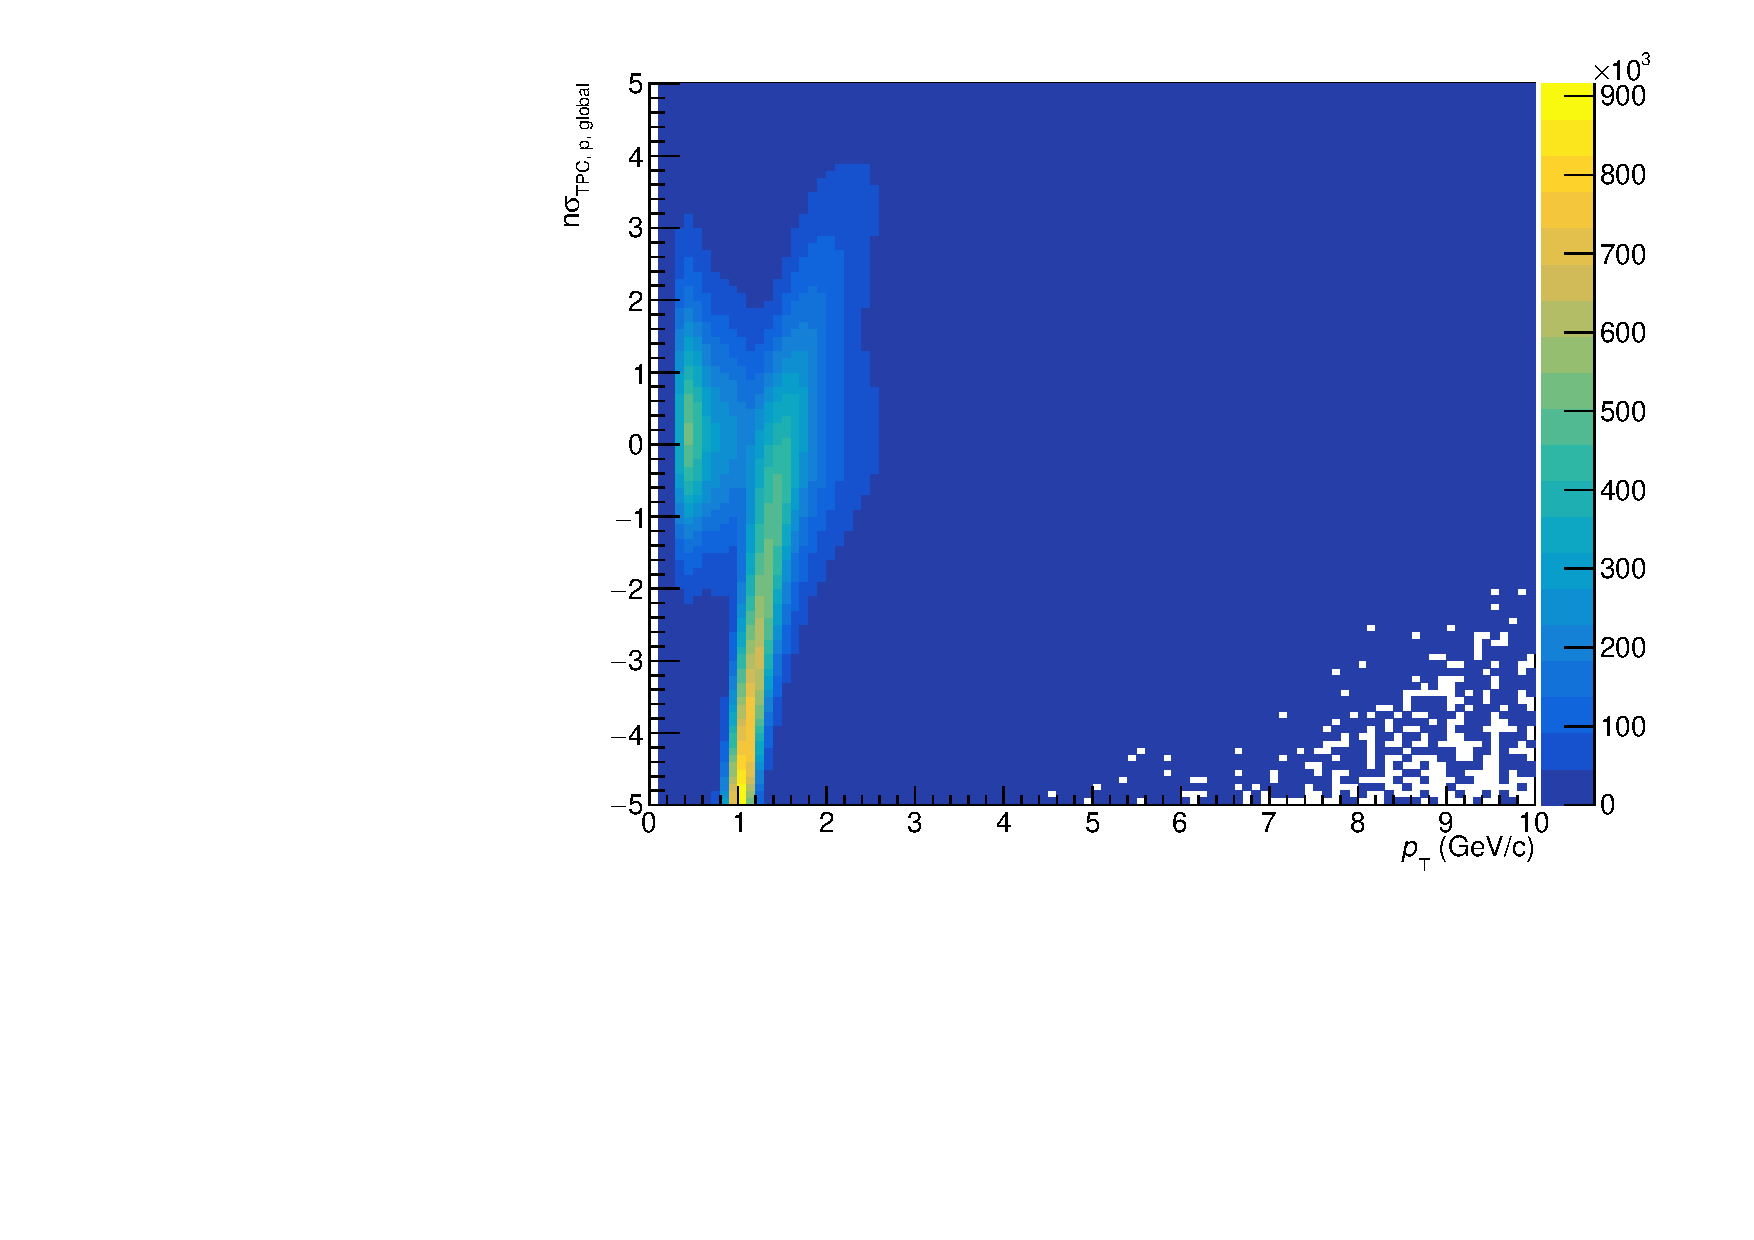
\includegraphics[width=3in]{figures/nsigma_tpc_proton_global.pdf}}
\end{subfigure}
\begin{subfigure}{
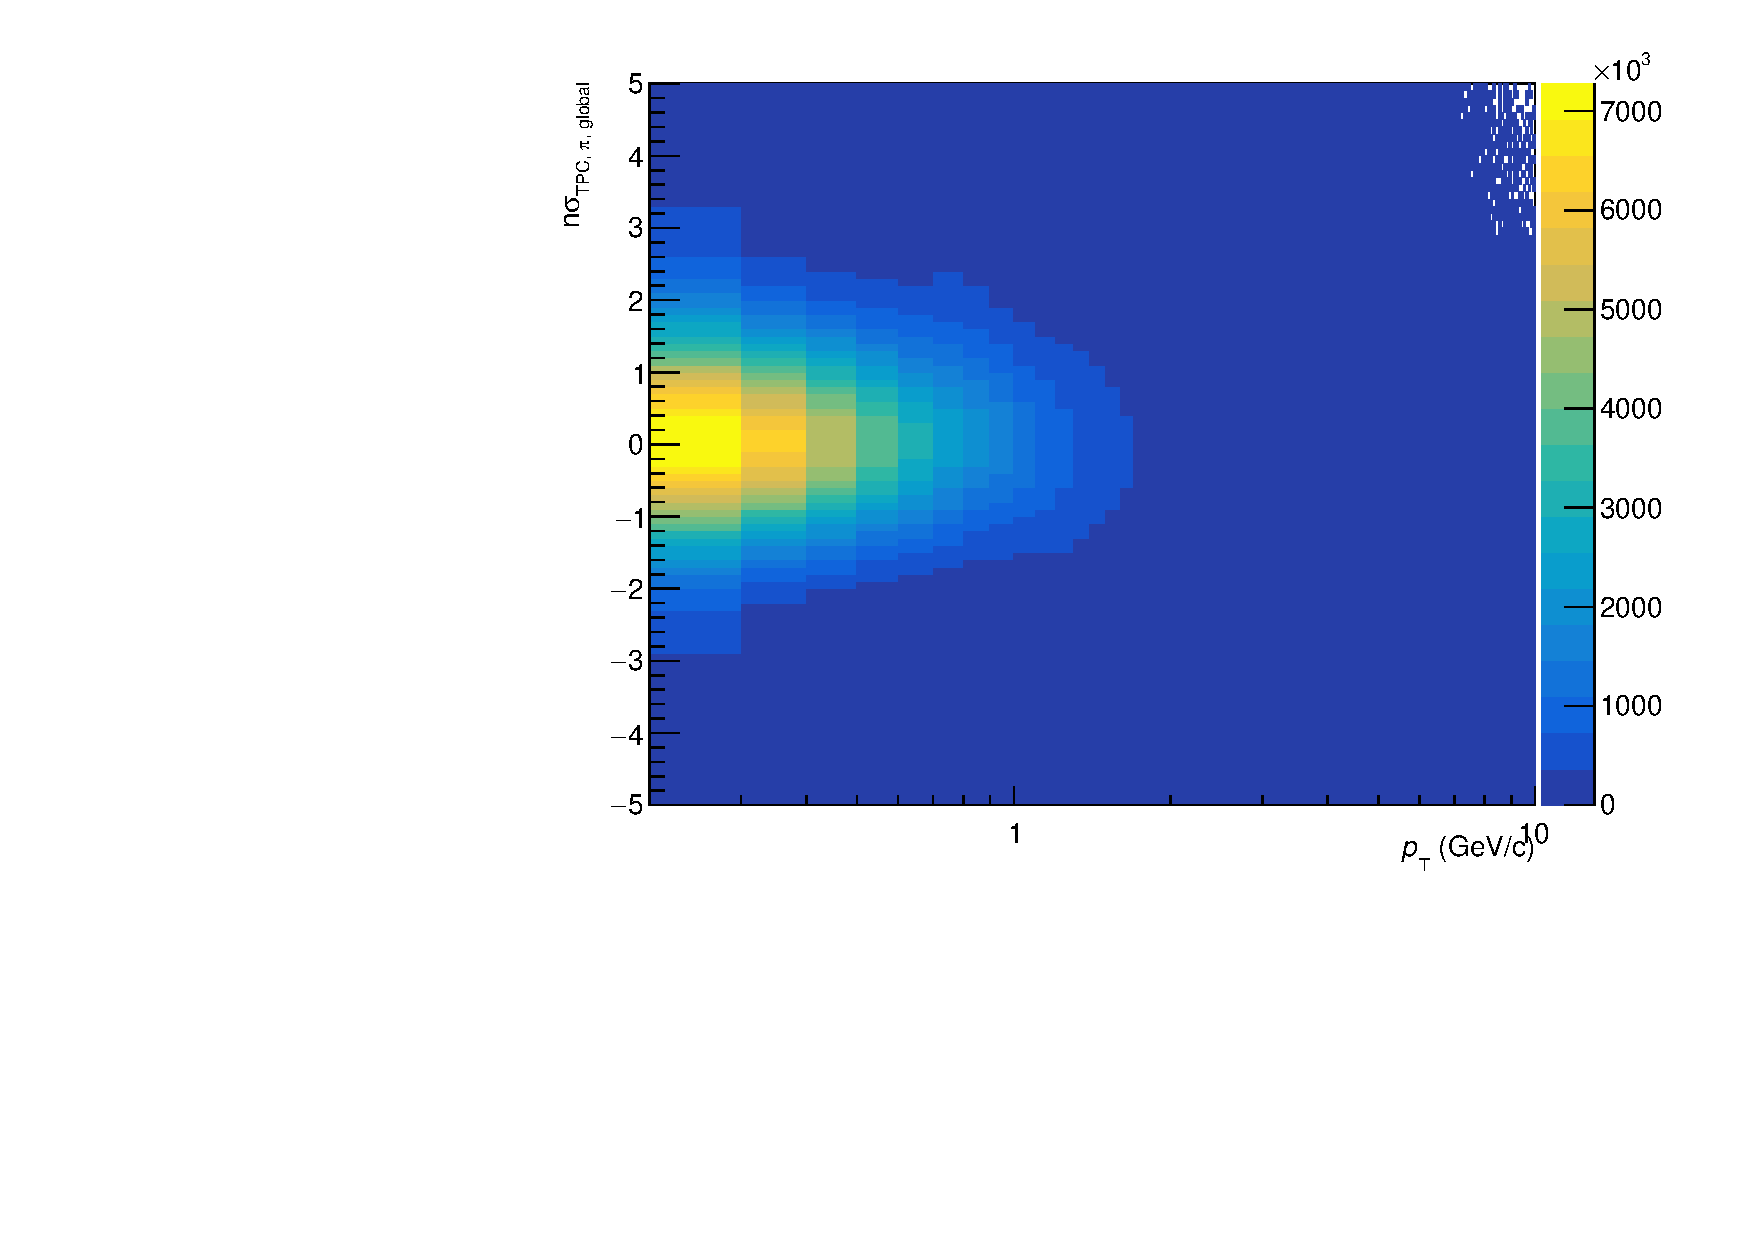
\includegraphics[width=3in]{figures/nsigma_tpc_pion_global.pdf}}
\end{subfigure}
\caption{$n\sigma$ for protons (left) and pions (right) from the global AOD track list in the TPC detector as a function of $p_{T}$. These plots are very similar to those generated from V0 daughter tracks, so we conclude no PID biases are introduced from the V0 finder method.}
\label{nsigma_tpc_global}
\end{figure}

\begin{figure}[ht]
\centering
\begin{subfigure}{
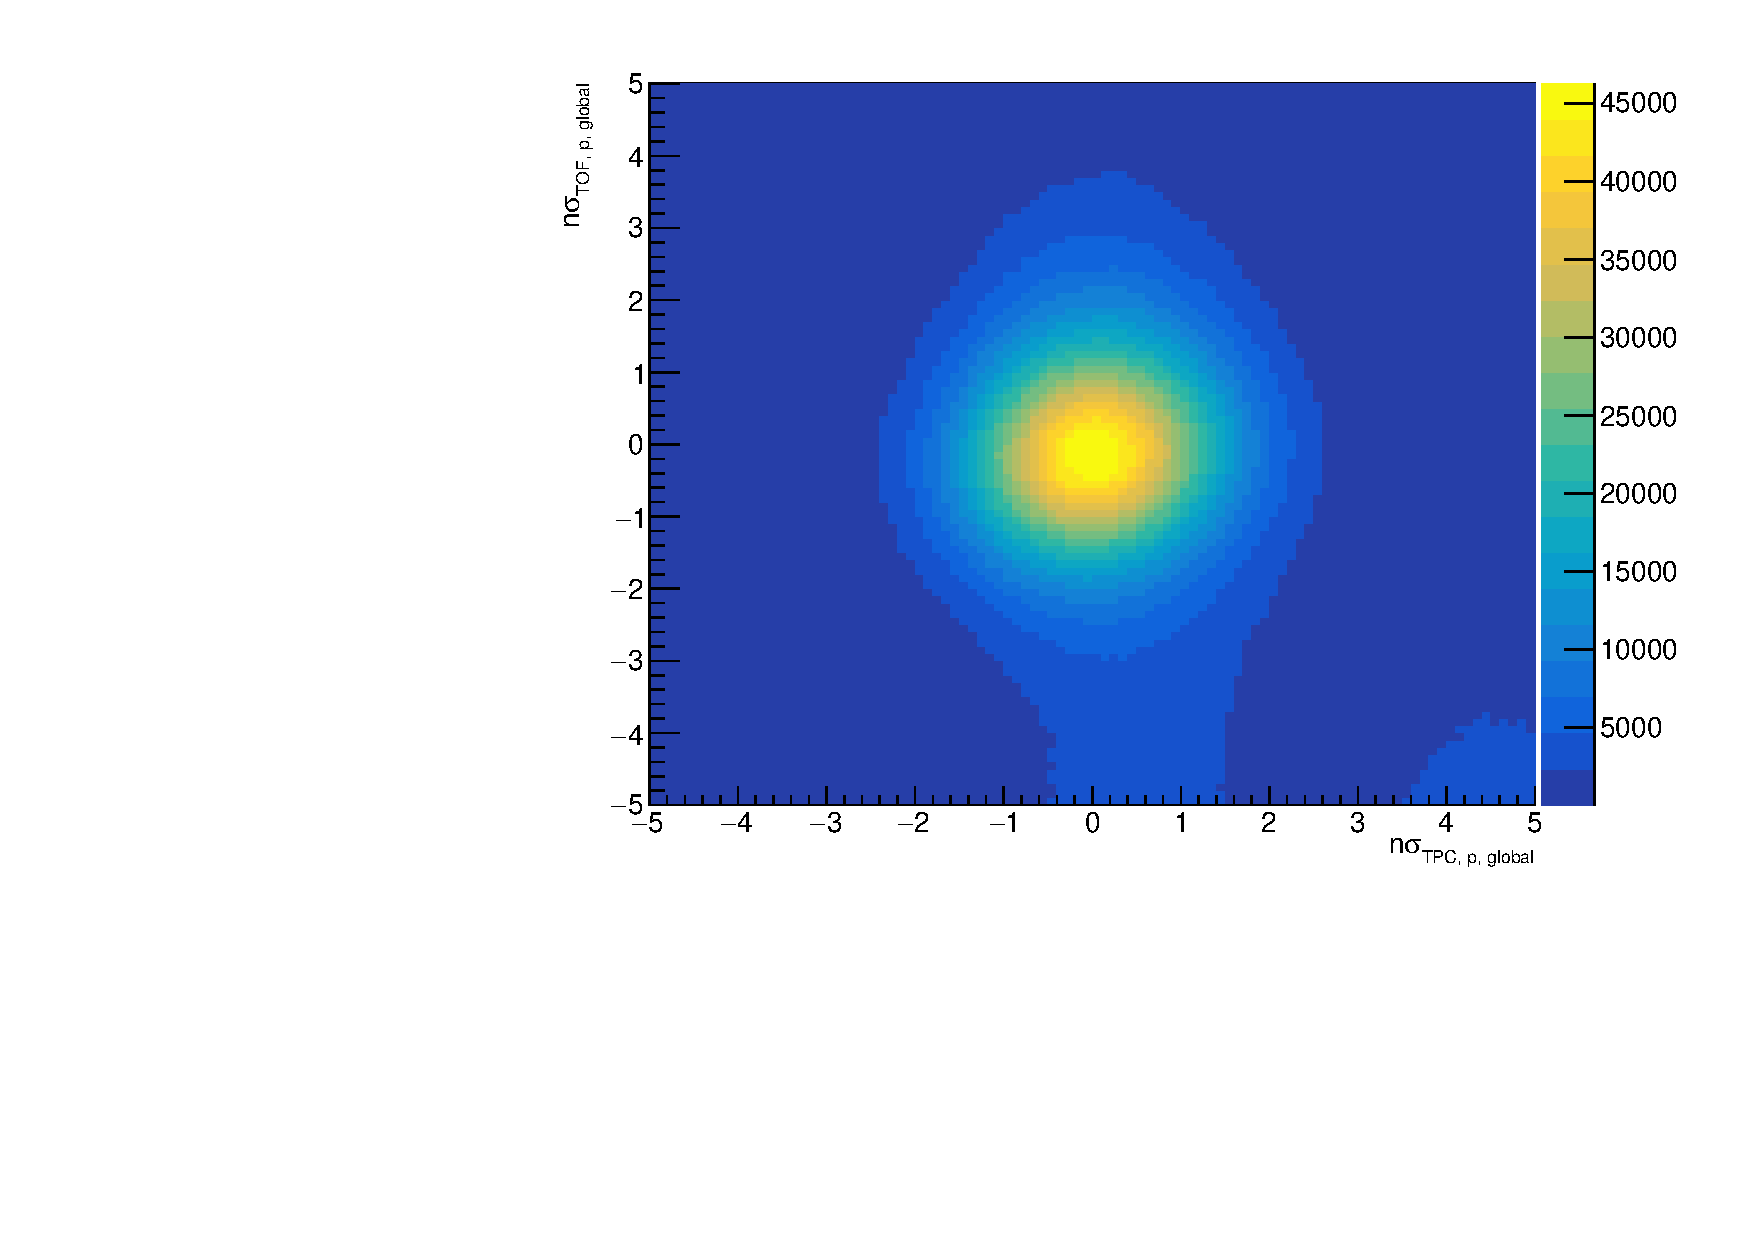
\includegraphics[width=3in]{figures/nsigma_tof_v_tpc_proton_global.pdf}}
\end{subfigure}
\begin{subfigure}{
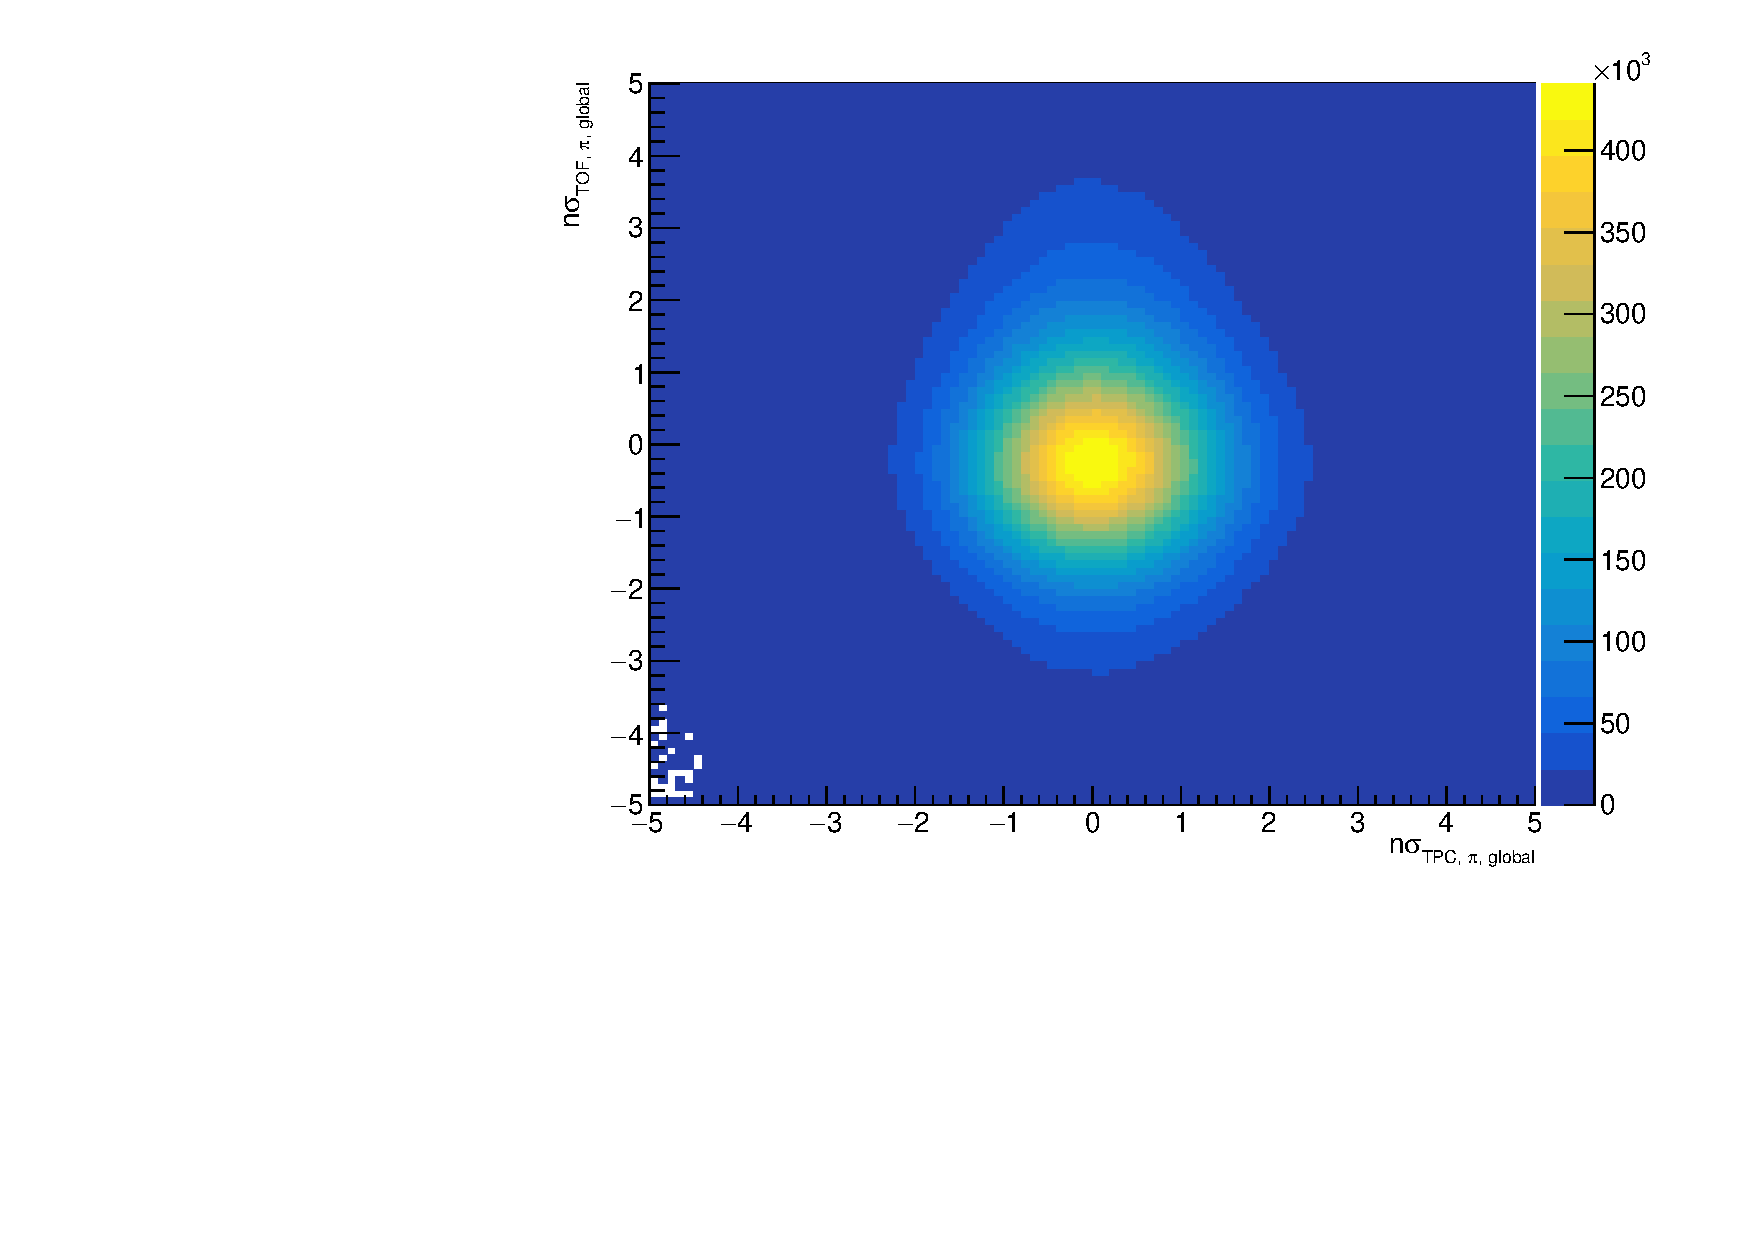
\includegraphics[width=3in]{figures/nsigma_tof_v_tpc_pion_global.pdf}}
\end{subfigure}
\caption{$n\sigma$ for protons (left) and pions (right) from the global AOD track list in the TOF detector as a function of $\it{p}_{T}$. Little to no contamination is observed.}
\label{nsigma_tof_global}
\end{figure}

\clearpage

 \subsection{Invariant Mass Regions}
 \label{invariant_mass_region}

 Measuring the $h-\Lambda$ correlation requires a clearly defined signal region for the unlike-sign $p\pi$ pairs from the V0 finder, as well as a sideband region to subtract any background contamination (see Section \ref{removecomb_v0} for more details). The $\Lambda$ invariant mass signal and sideband regions for the central points of this analysis are as follows:
\begin{itemize}
	\item \makebox[7.5cm][l]{Signal region}  \SI{1.102}{GeV/c^2}$< M_{p\pi} < $\SI{1.130}{GeV/c^2}
	\item \makebox[7.5cm][l]{Sideband region}  \SI{1.135}{GeV/c^2}$< M_{p\pi} < $\SI{1.150}{GeV/c^2}
\end{itemize}

Both the signal and sideband regions are varied as a systematic check (see Section \ref{systematics})
The invariant mass distributions in each multiplicity bin for the $\Lambda$s reconstructed using the V0 finder algorithm in events with a trigger hadron are shown in Figures \ref{v0_mass} to \ref{v0_mass_highpt}. The $\Lambda$ peak is clearly visible with very little background. A Voigt (signal) + straight line (background) fit was applied to the invariant mass distributions for each multiplicity bin. The extracted parameters from the Voigt fit are shown in Table \ref{voigt_parameters}. In the end, the Voigt fit is only shown for aesthetic purposes. While the background is very small for each multiplicity bin, it is still subtracted from our final $h-\Lambda$ correlation distribution using the procedure described in Section \ref{removecomb_v0}, which relies only on the background fit. It should also be mentioned that the background line (shown as the purple dashed line) is fixed at the ends to the points where we expect no signal (verified in MonteCarlo, as the signal shapes in data and MonteCarlo are very similar).

\begin{table}[h!]
\centering
\begin{tabular}{| c || c | c | c | c | c | }
\hline
Multiplicity & A & $\mu$ (GeV/$c^2$) & $\sigma$ (GeV/$c^2$) & $\gamma$ (GeV/$c^2$) & $\chi^2$/NDF \\
\hline
0-20\% & 1.82e+02  & 1.116 & 1.24e-03 & 1.10e-03 & 31.24\\
20-50\% & 8.58e+01 & 1.116 & 1.24e-03 & 1.07e-03 & 15.55\\
50-80\% & 1.78e+01 & 1.116 & 1.23e-03 & 1.03e-03 & 4.55\\
\hline
\end{tabular}
\caption{Parameters from the Voigt fit to the invariant mass distributions for the $\Lambda$s reconstructed using the V0 finder in events with a trigger hadron, along with the $\chi^2/NDF$ for the total fit. The errors were negligible relative to the values.}
\label{voigt_parameters}
\end{table}

\clearpage
 
\begin{figure}[ht]
\centering
\begin{subfigure} {
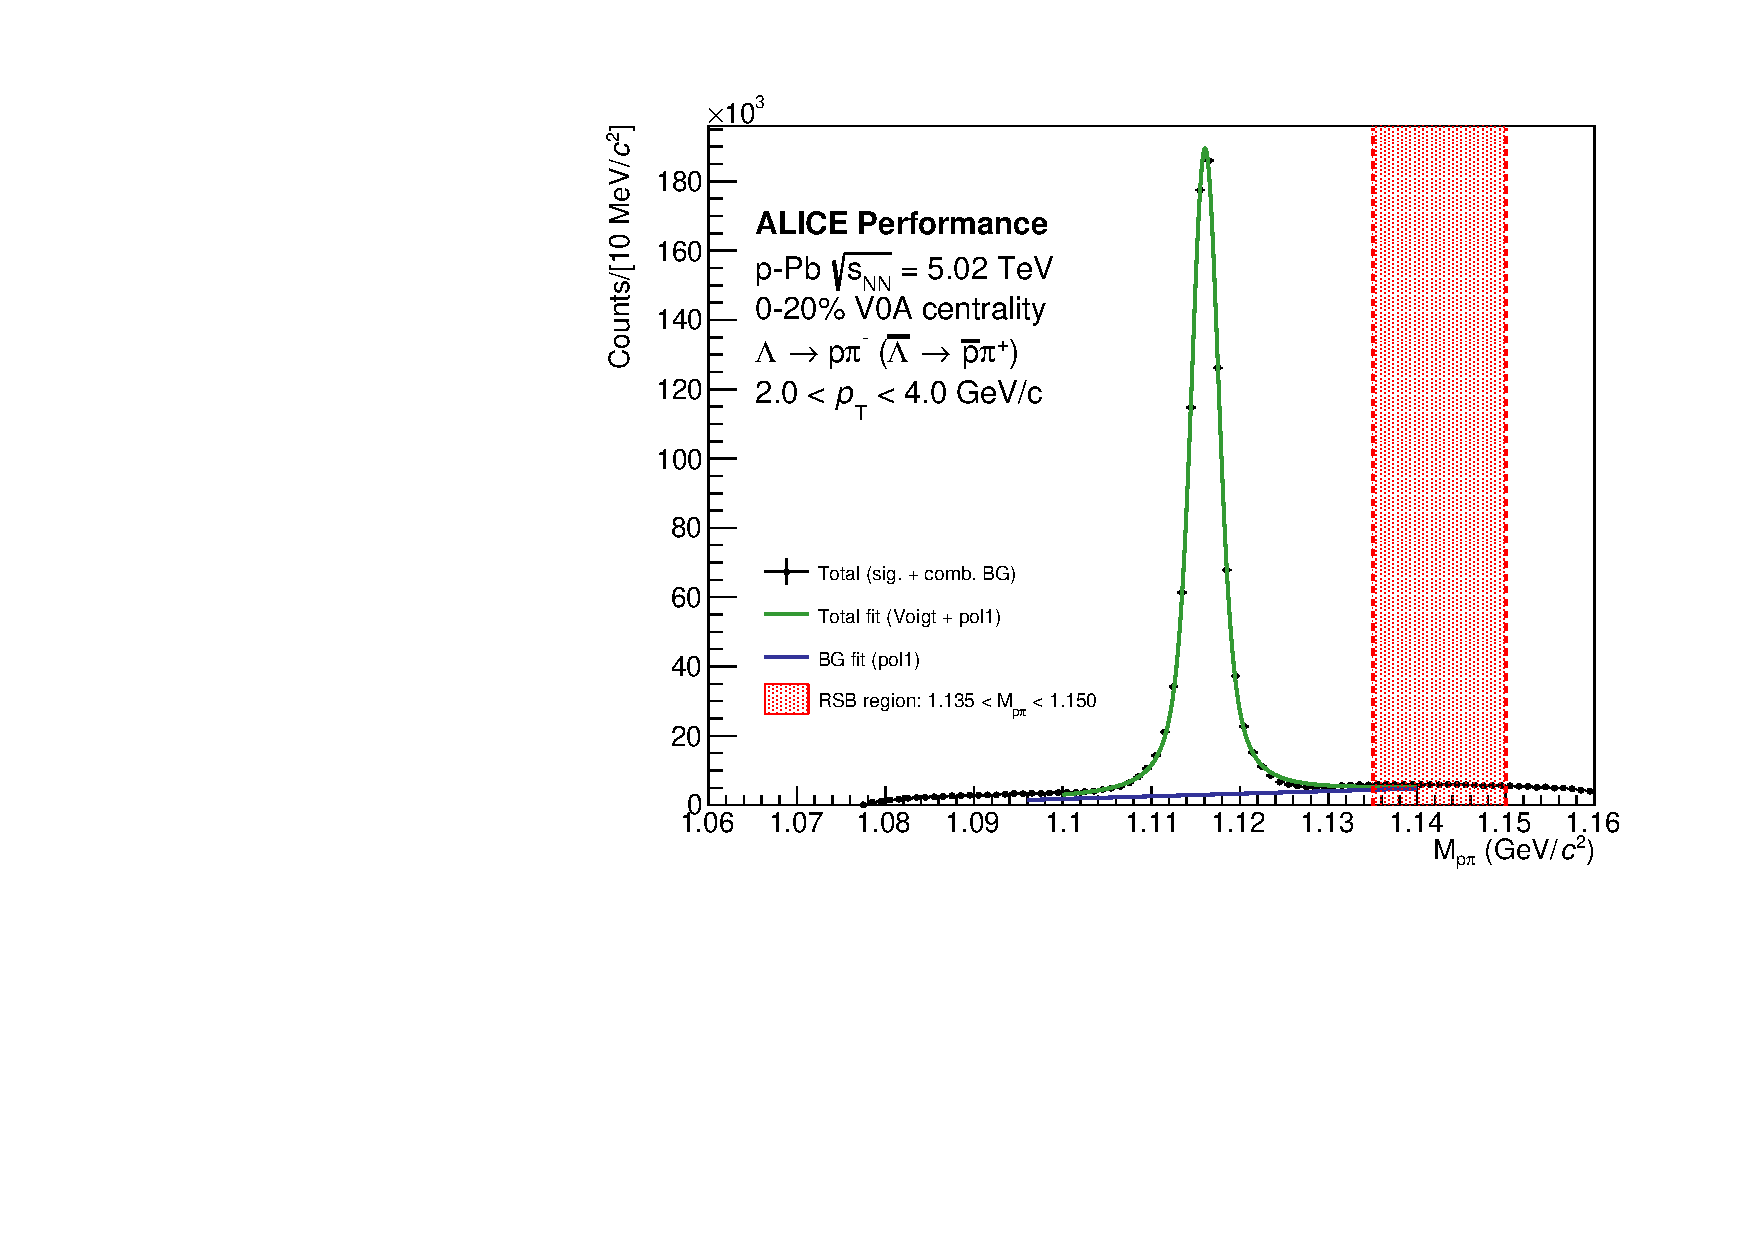
\includegraphics[width=4in]{figures/lambda_mass_dist_0_20.pdf}}
\end{subfigure}
\begin{subfigure} {
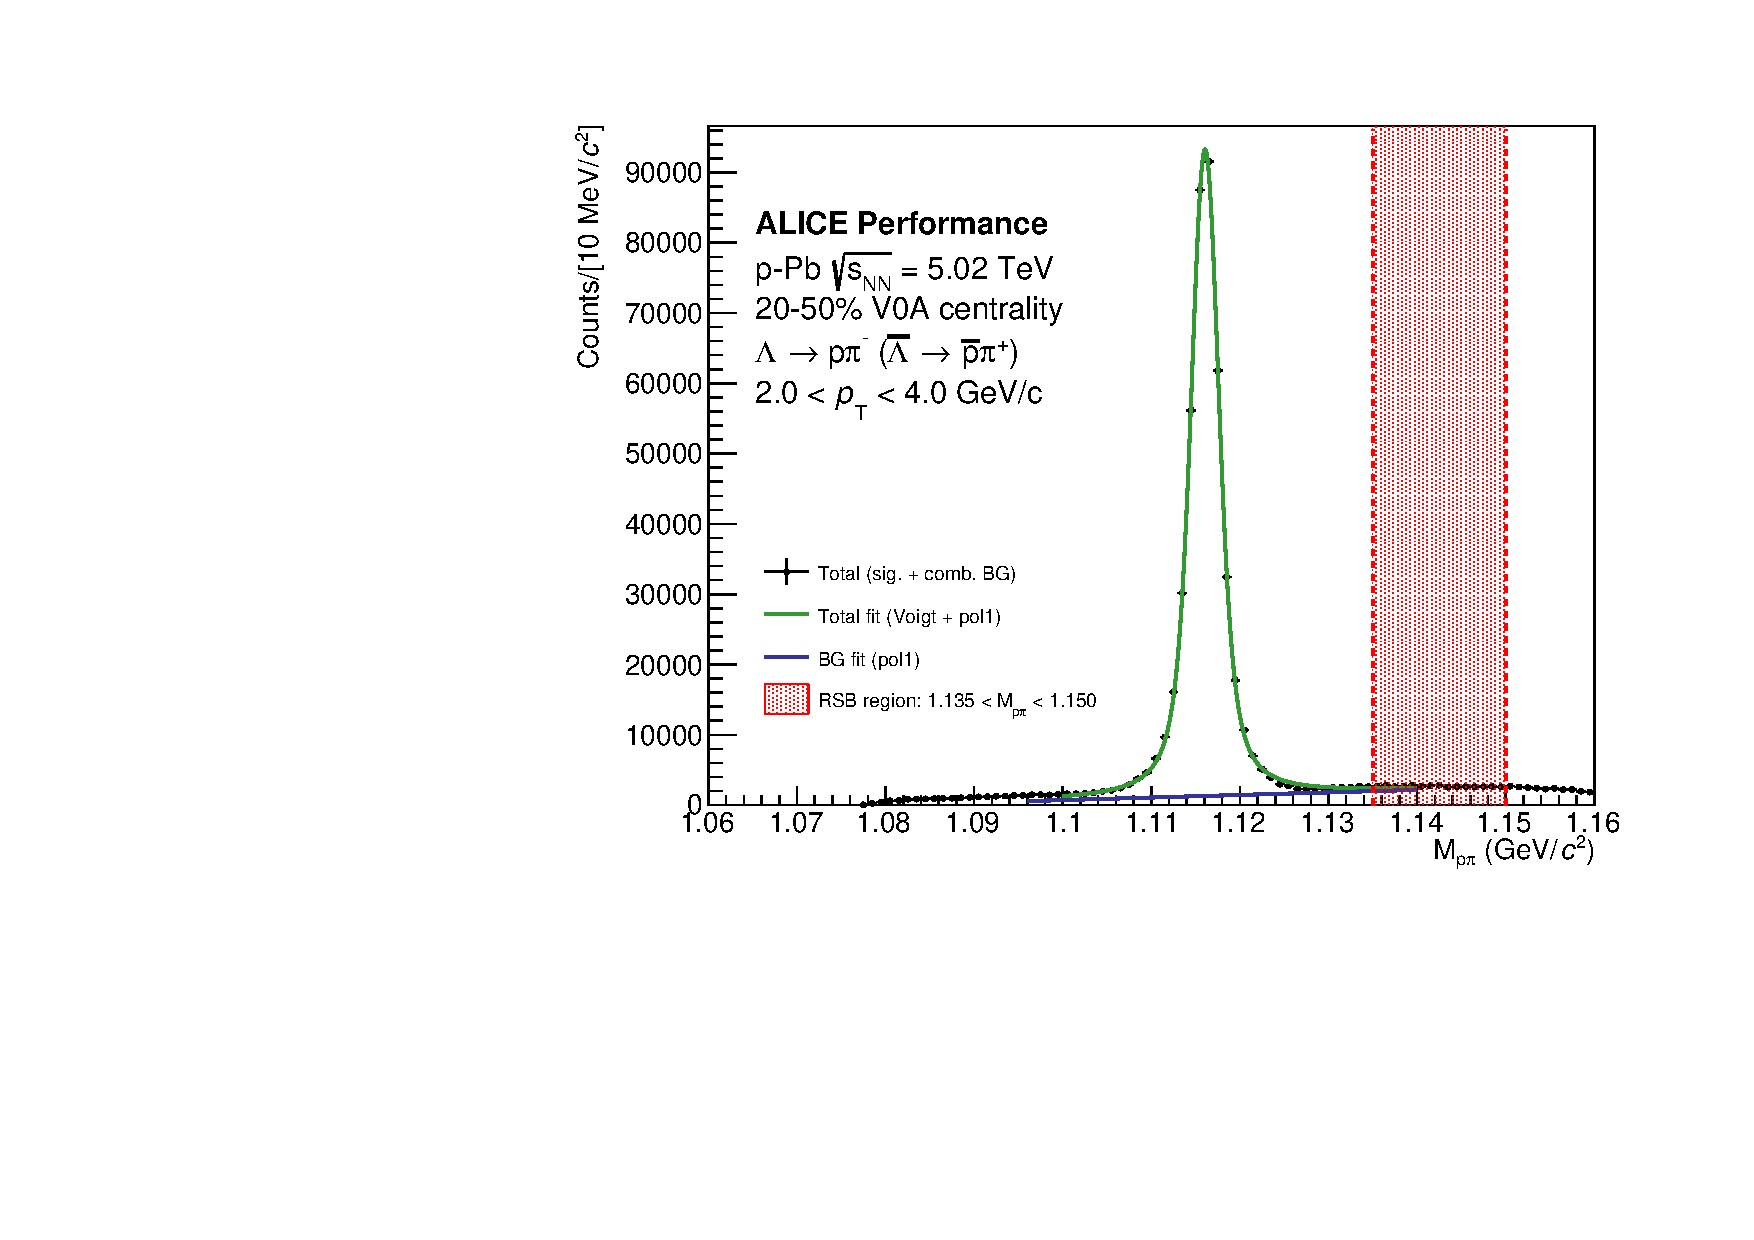
\includegraphics[width=4in]{figures/lambda_mass_dist_20_50.pdf}}
\end{subfigure}
\begin{subfigure} {
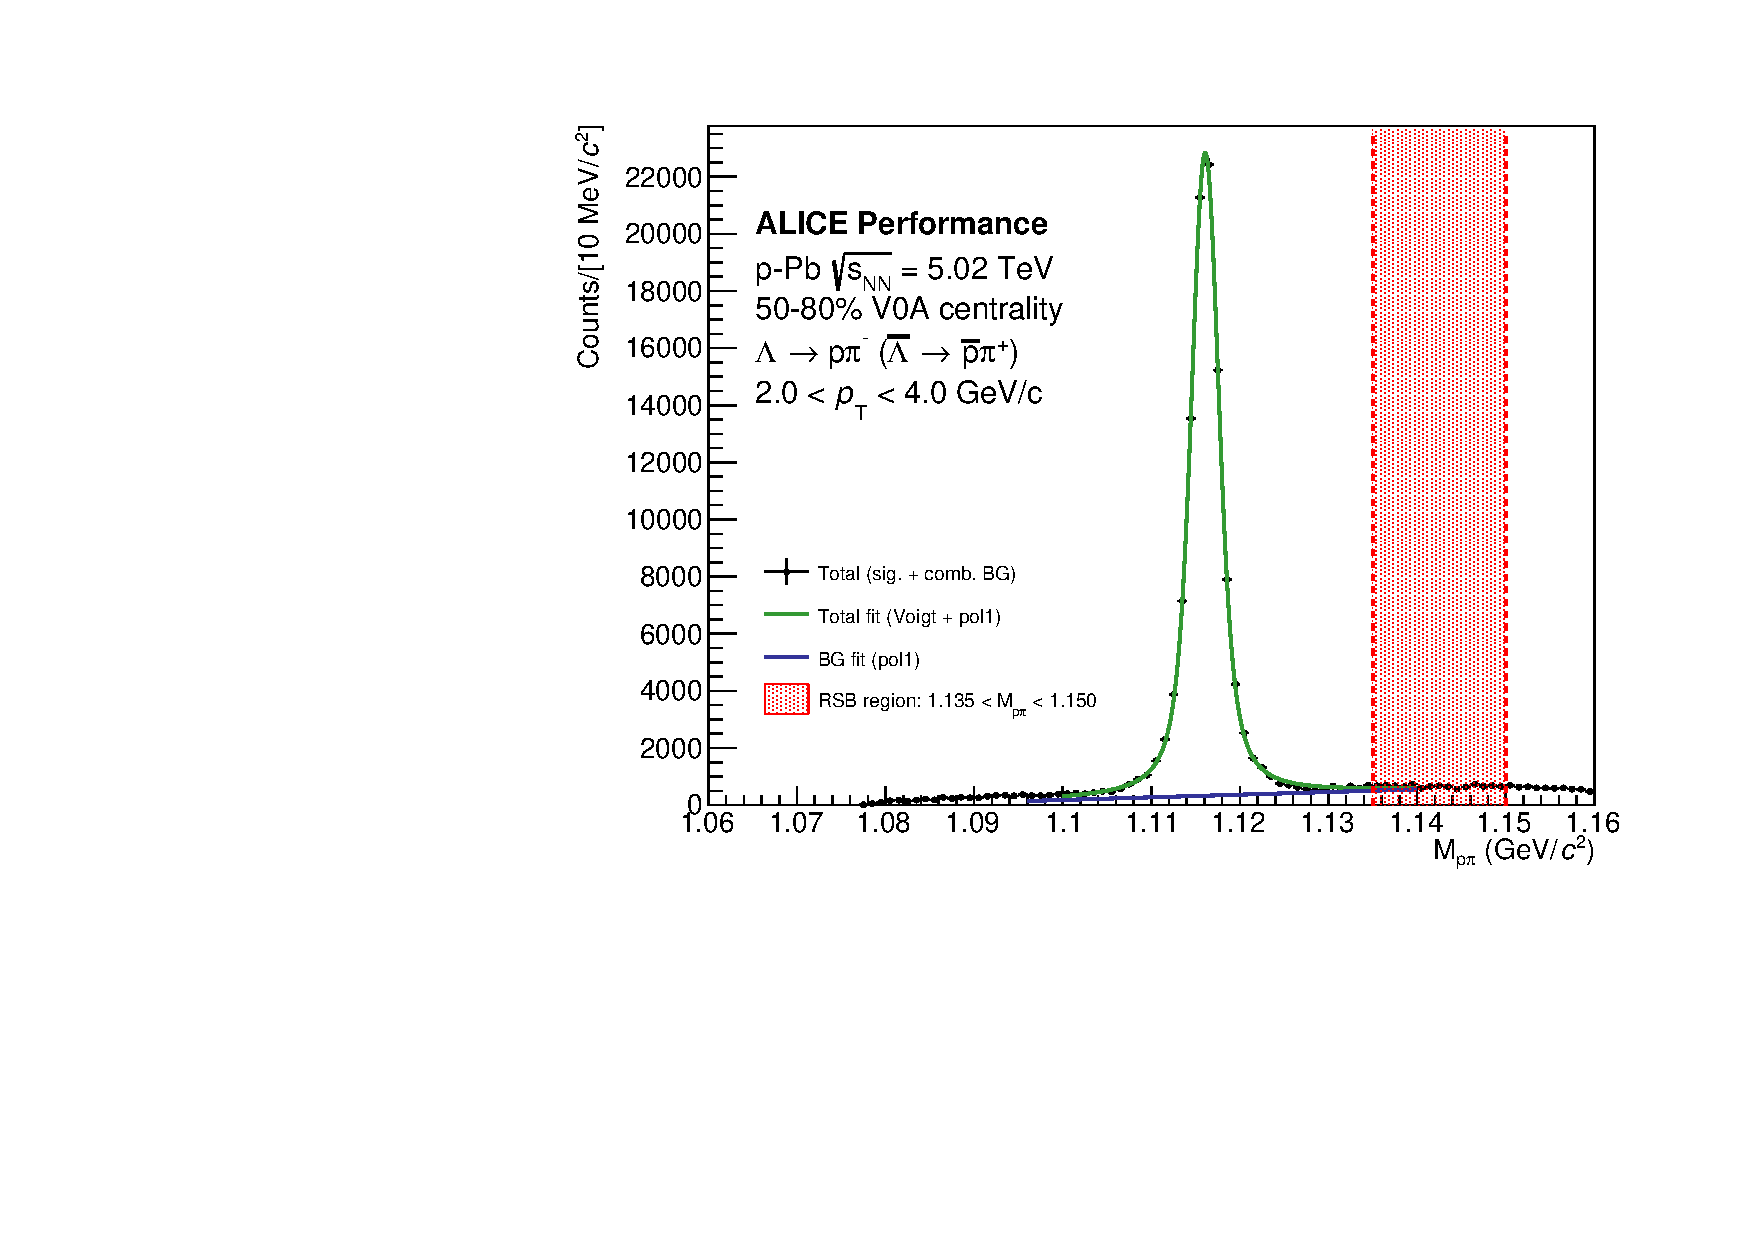
\includegraphics[width=4in]{figures/lambda_mass_dist_50_80.pdf}}
\end{subfigure}
\caption{Invariant mass distributions in the 0-20\% (top), 20-50\% (center), and 50-80\% (bottom) multiplicity bins for $\Lambda$s reconstructed using the V0 finder in events with a trigger hadron with $2 < \it{p}_T < 4$. The background from misidentified $\Lambda$s is small for all multiplicity bins.}
\label{v0_mass}
\end{figure}

\clearpage

\begin{figure}[ht]
\centering
\begin{subfigure} {
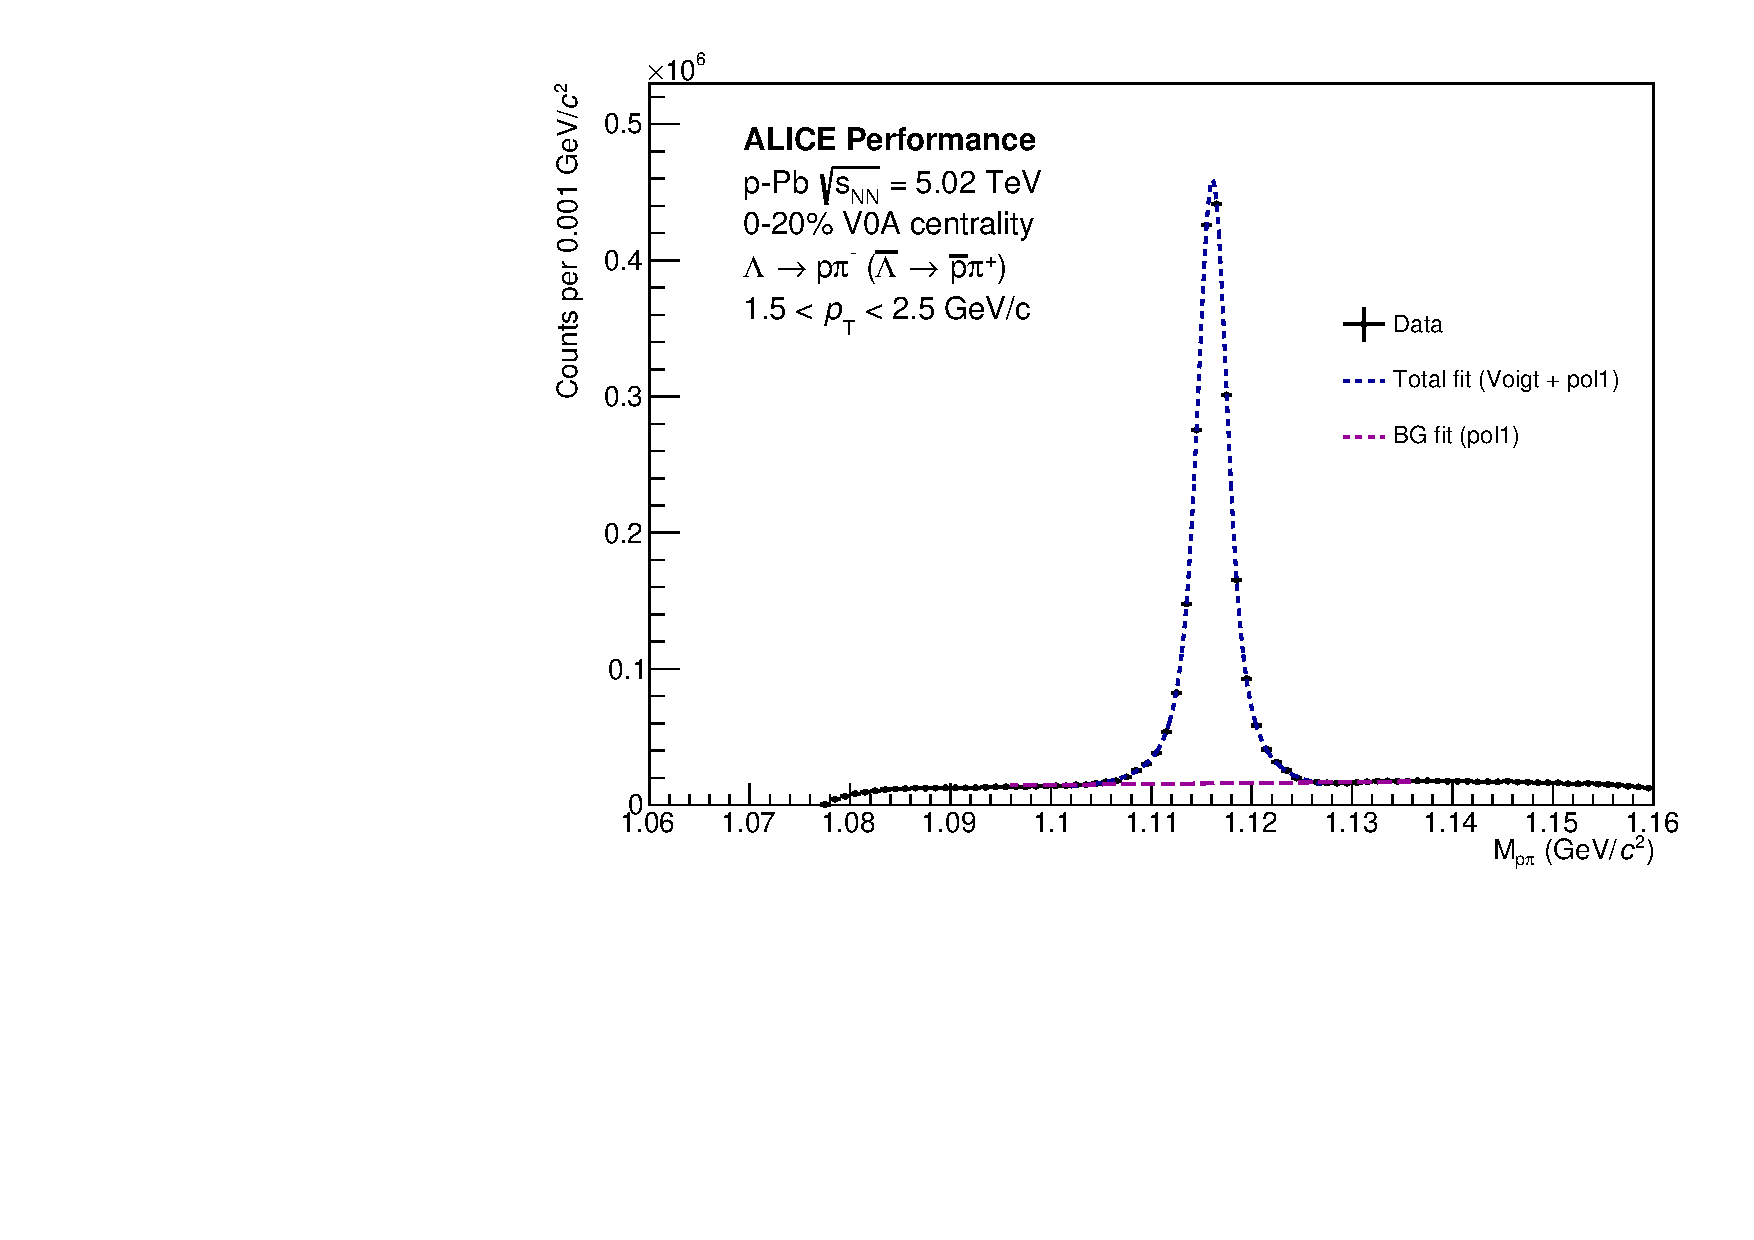
\includegraphics[width=4in]{figures/lambda_mass_dist_0_20_lowpt.pdf}}
\end{subfigure}
\begin{subfigure} {
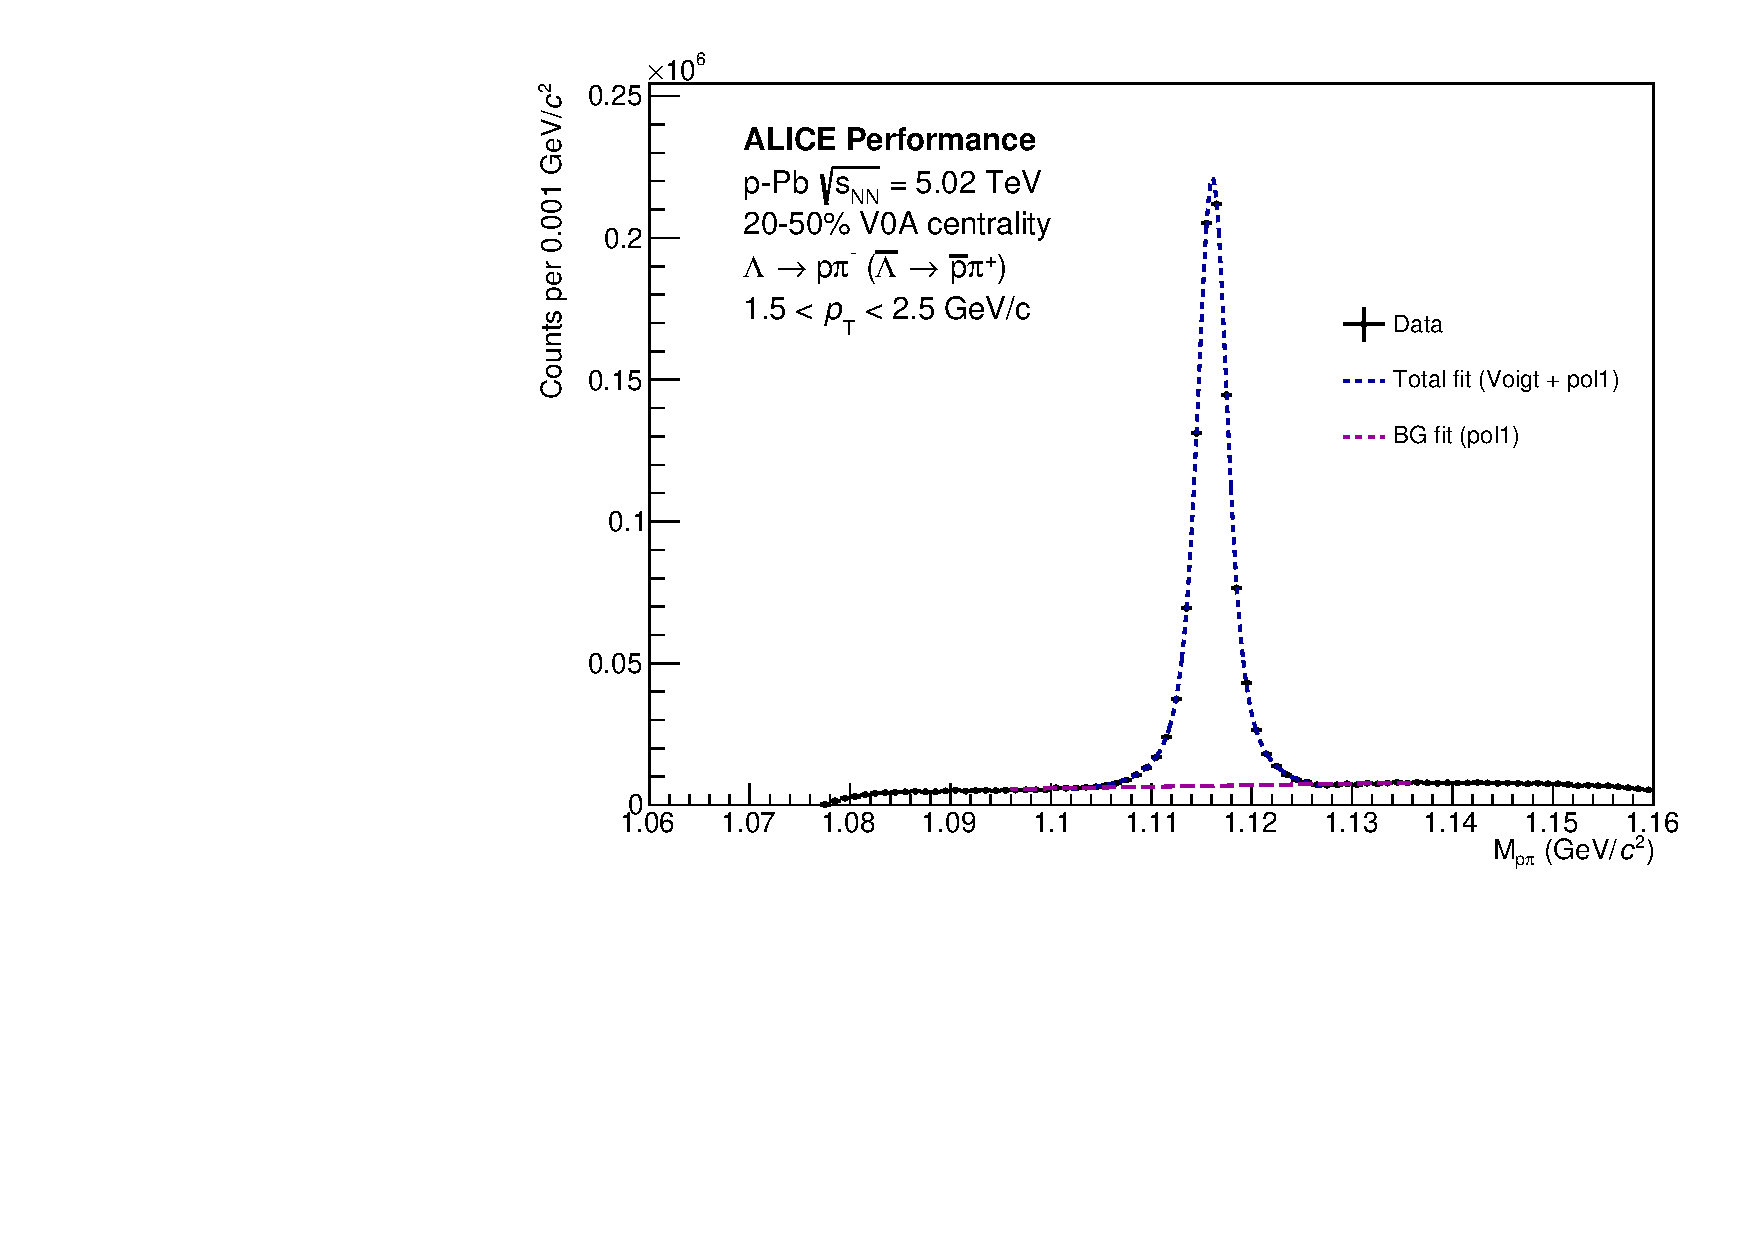
\includegraphics[width=4in]{figures/lambda_mass_dist_20_50_lowpt.pdf}}
\end{subfigure}
\begin{subfigure} {
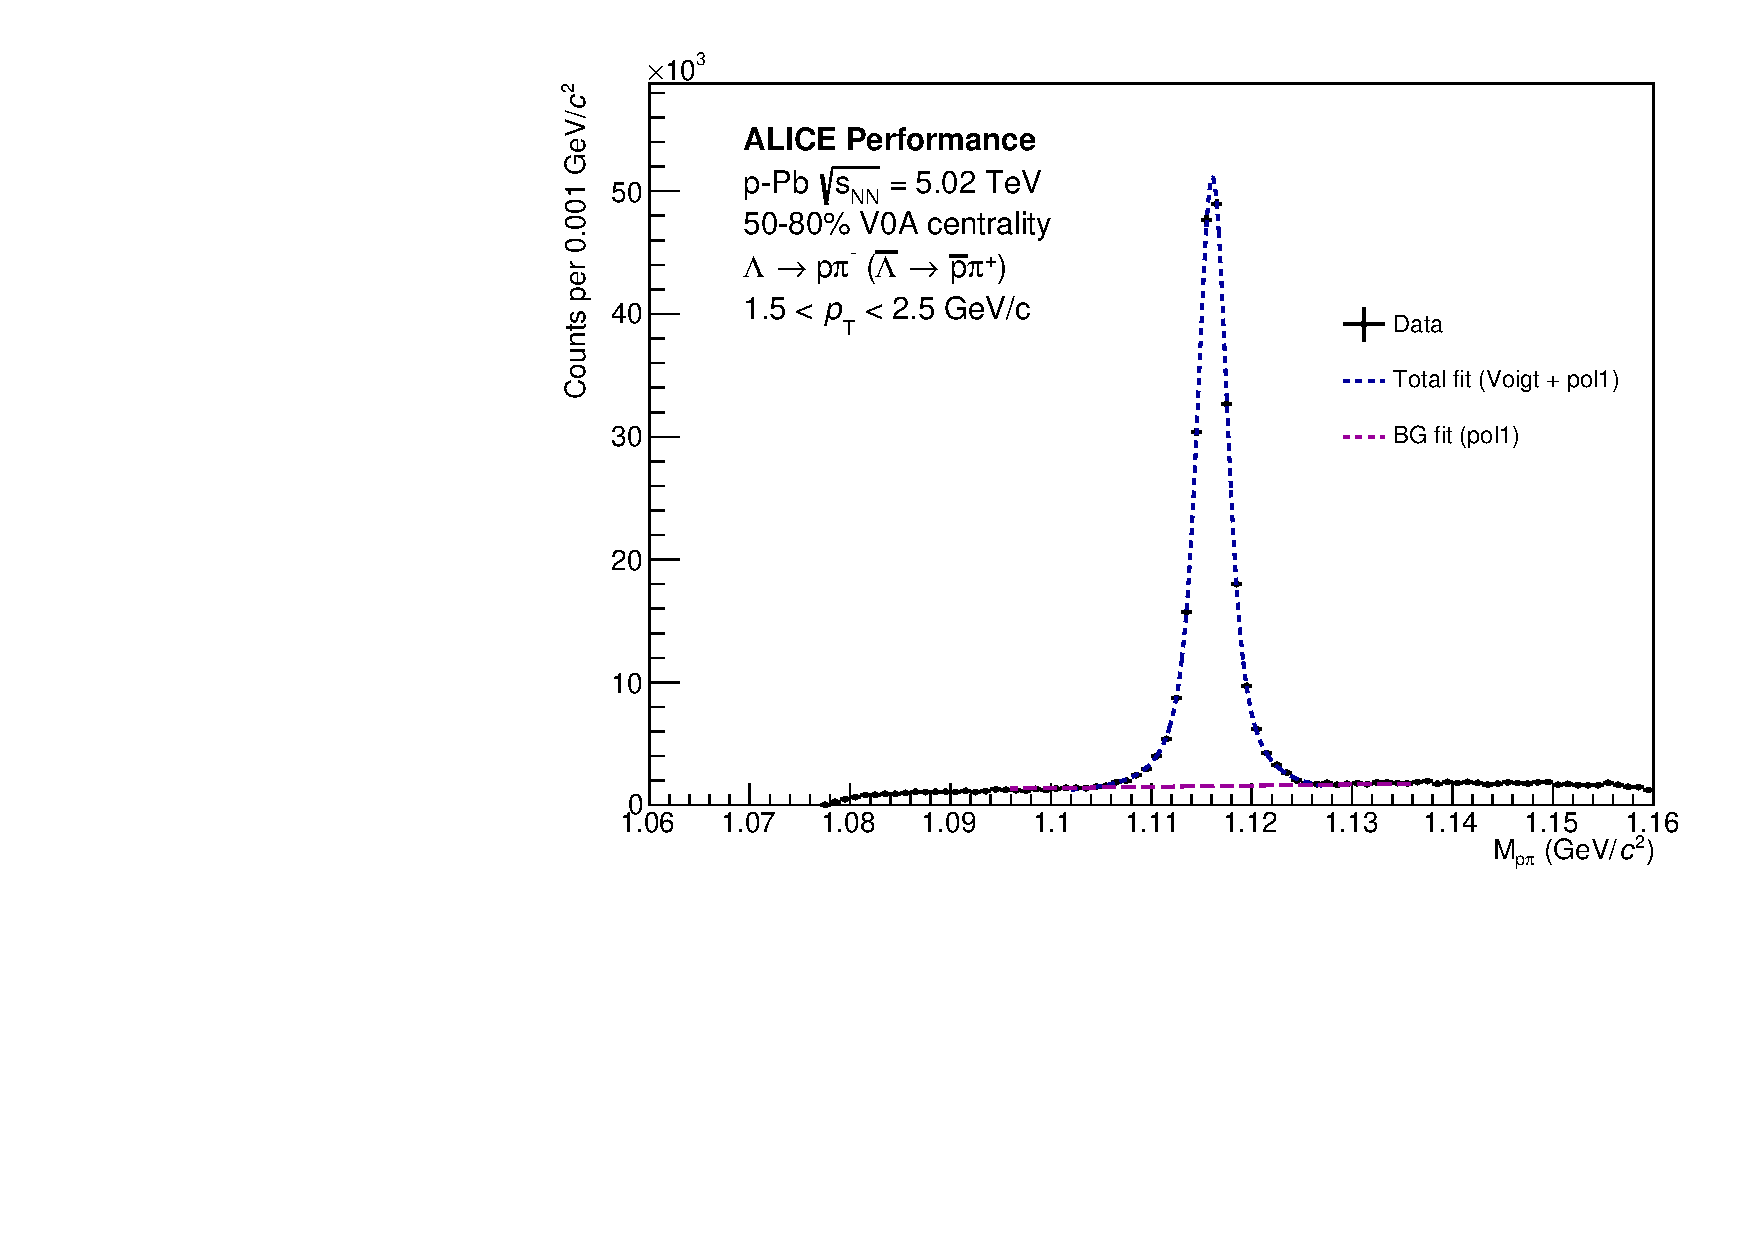
\includegraphics[width=4in]{figures/lambda_mass_dist_50_80_lowpt.pdf}}
\end{subfigure}
\caption{Invariant mass distributions in the 0-20\% (top), 20-50\% (center), and 50-80\% (bottom) multiplicity bins for $\Lambda$s reconstructed using the V0 finder in events with a trigger hadron with $1.5 < \it{p}_T < 2.5$. The background from misidentified $\Lambda$s is small for all multiplicity bins, but it is larger than our higher $p_{T}$ bin.}
\label{v0_mass_lowpt}
\end{figure}

\clearpage

\begin{figure}[ht]
\centering
\begin{subfigure} {
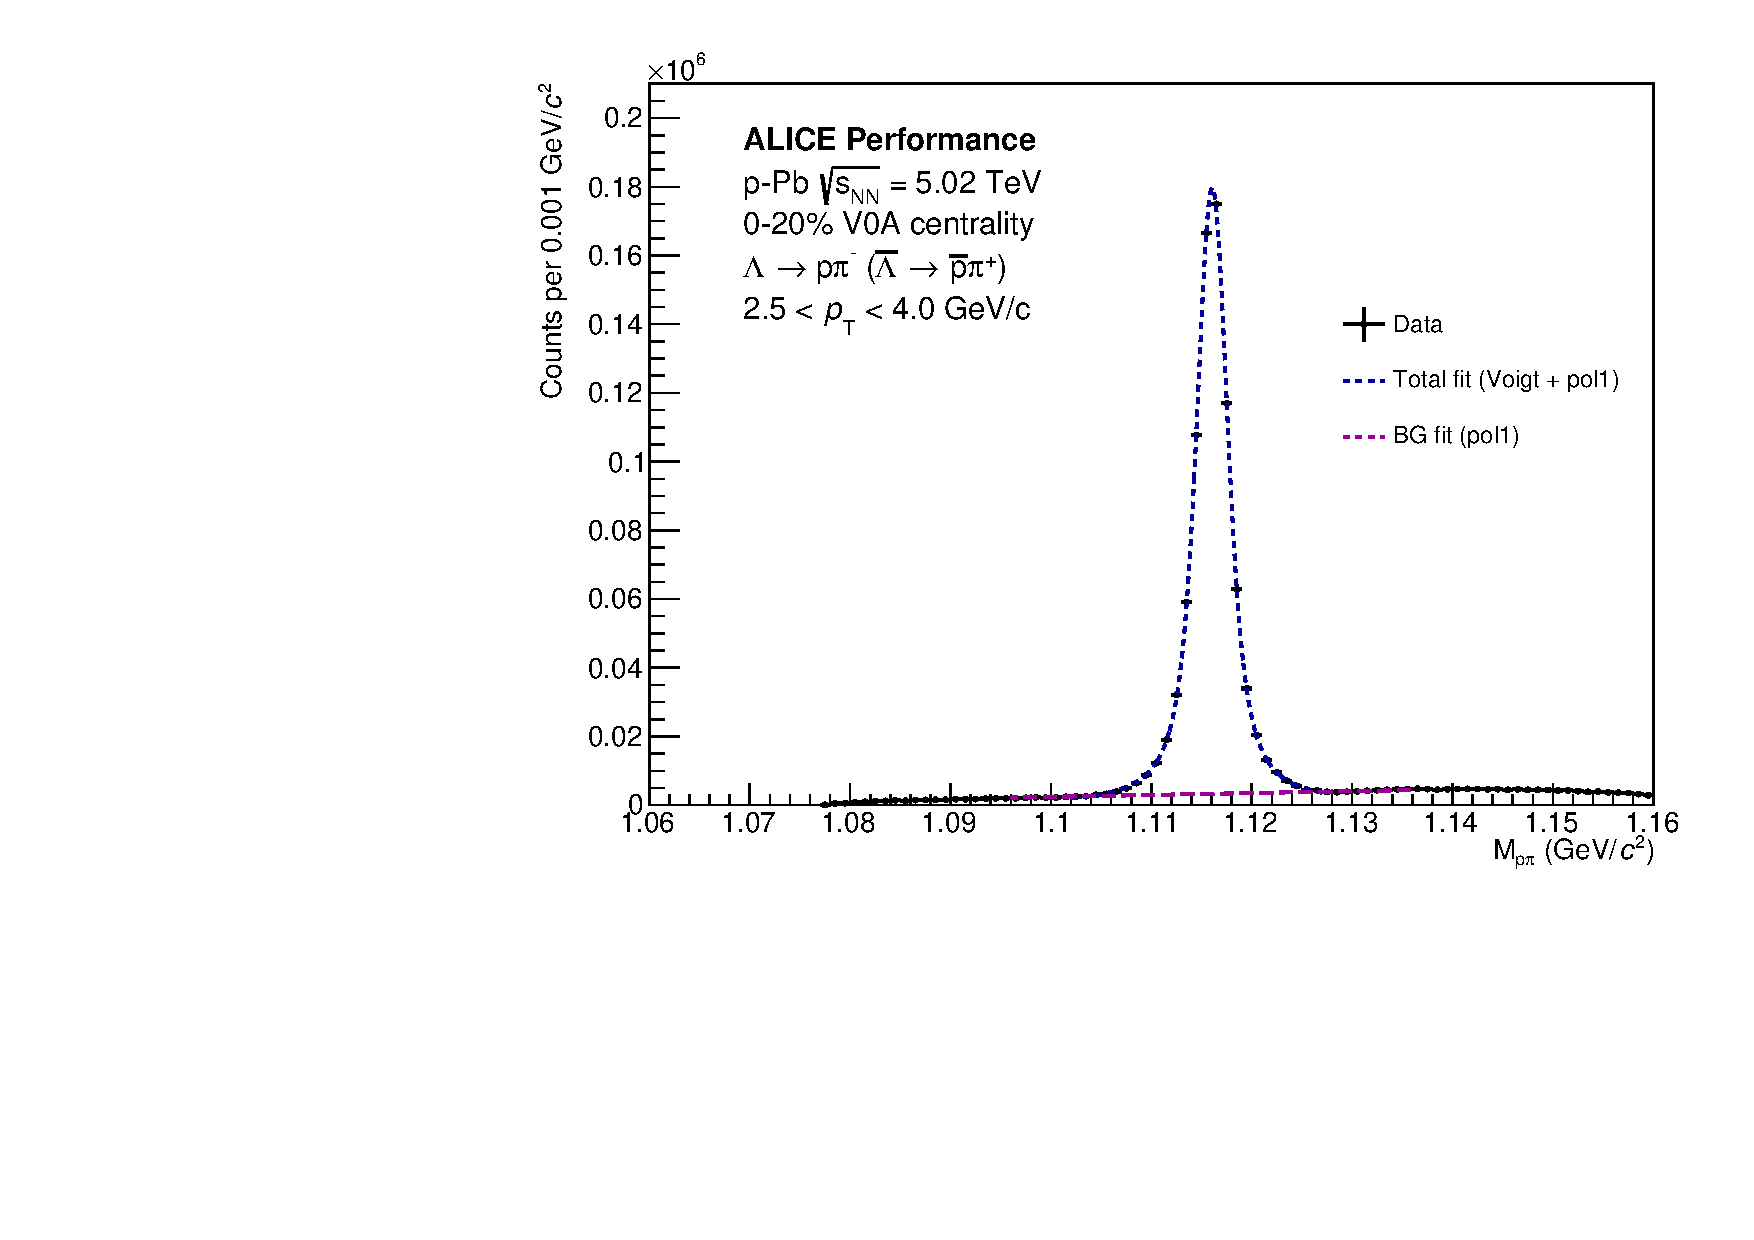
\includegraphics[width=4in]{figures/lambda_mass_dist_0_20_highpt.pdf}}
\end{subfigure}
\begin{subfigure} {
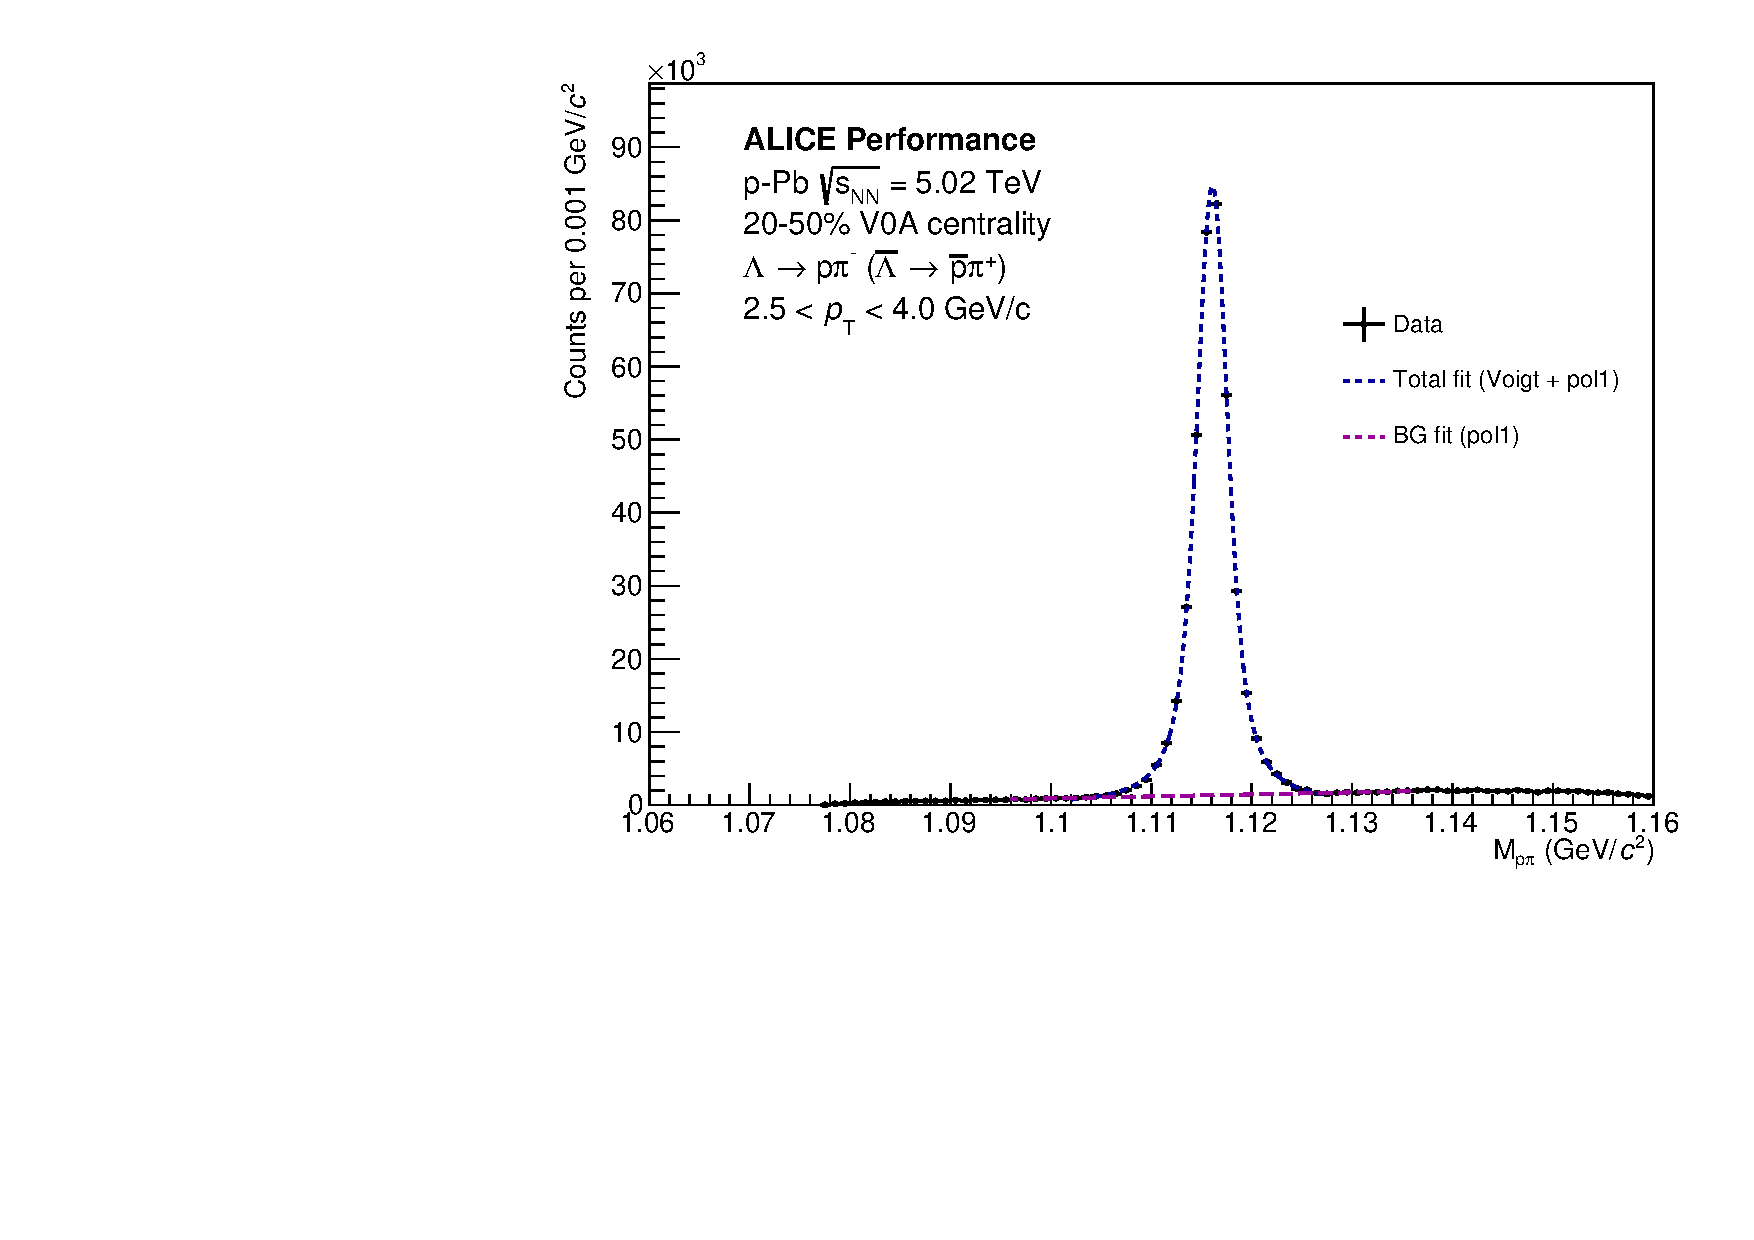
\includegraphics[width=4in]{figures/lambda_mass_dist_20_50_highpt.pdf}}
\end{subfigure}
\begin{subfigure} {
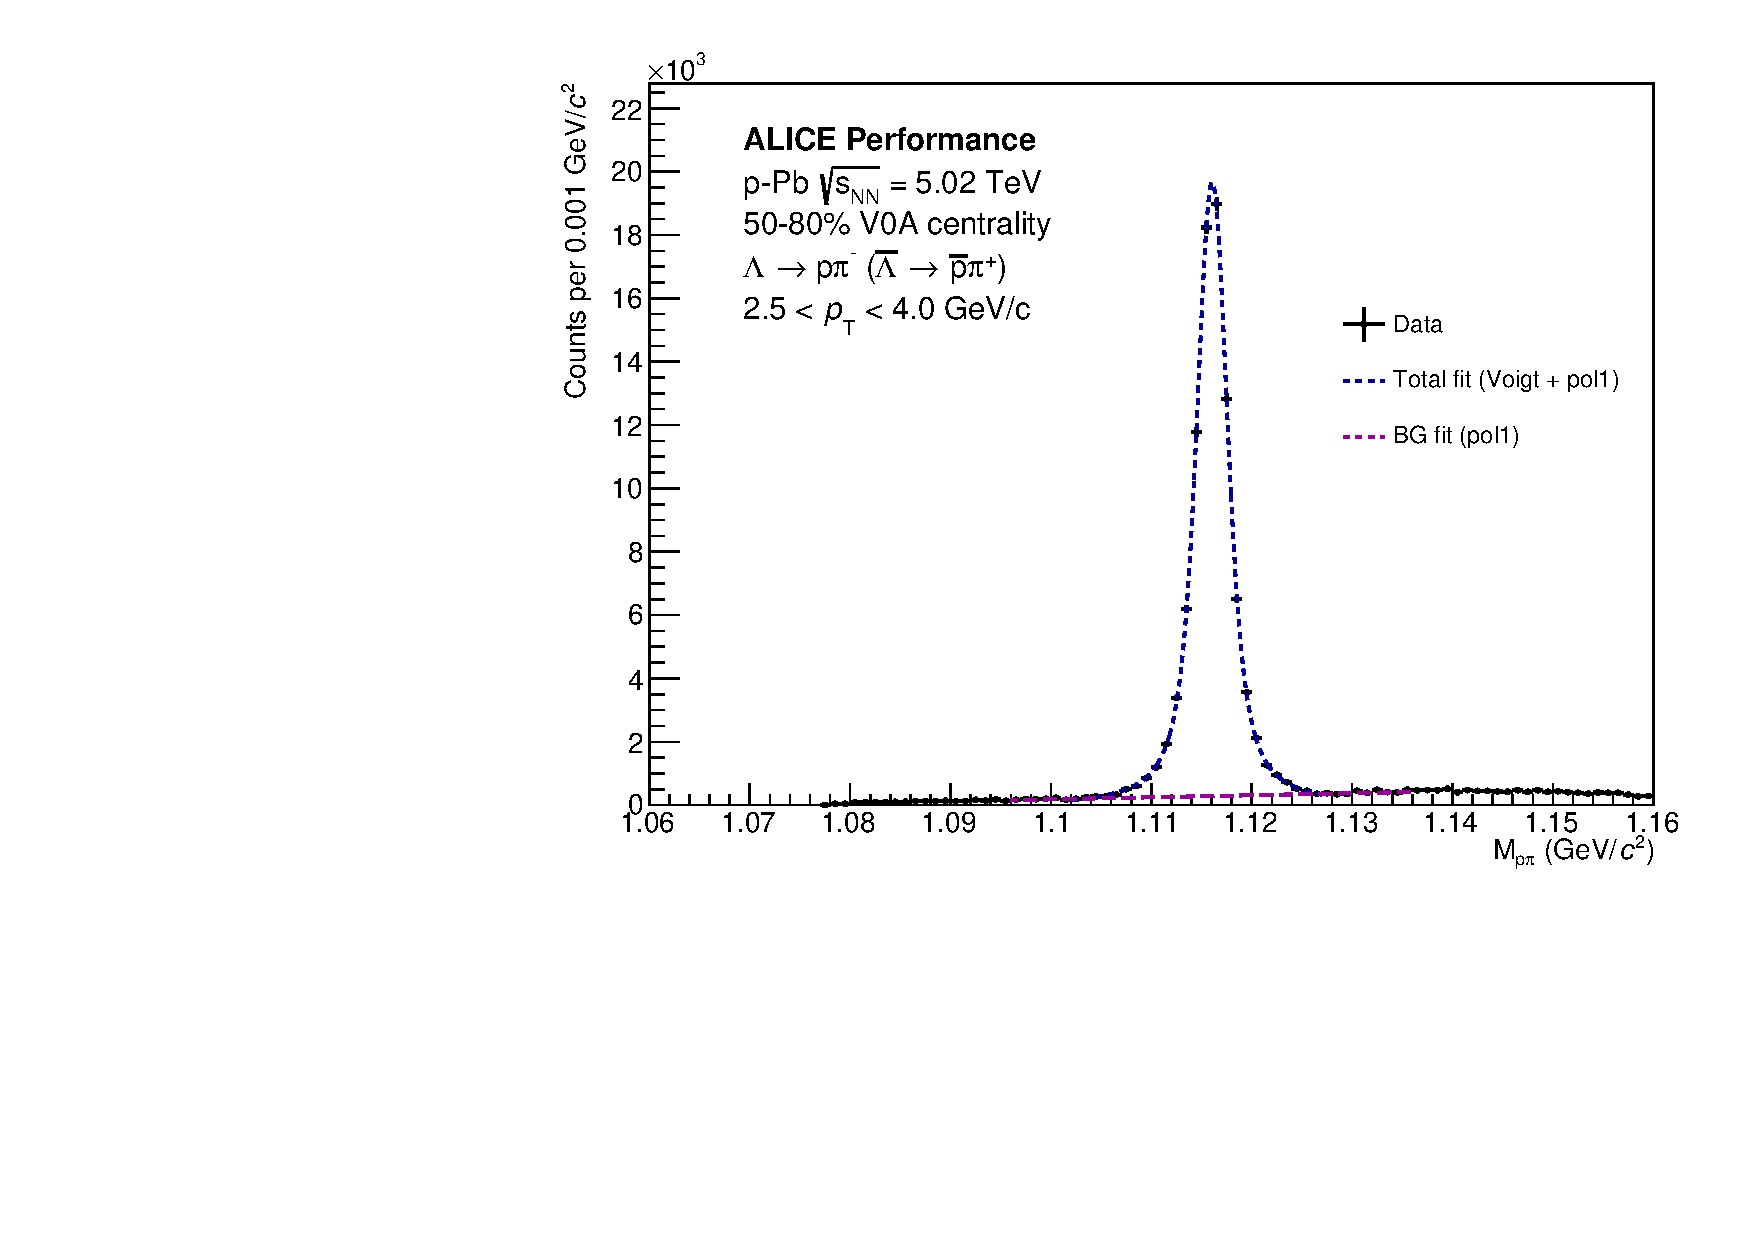
\includegraphics[width=4in]{figures/lambda_mass_dist_50_80_highpt.pdf}}
\end{subfigure}
\caption{Invariant mass distributions in the 0-20\% (top), 20-50\% (center), and 50-80\% (bottom) multiplicity bins for $\Lambda$s reconstructed using the V0 finder in events with a trigger hadron with $2.5 < \it{p}_T < 4$. The background from misidentified $\Lambda$s is the smallest for all multiplicity bins when compared to our other $p_{T}$ bins.}
\label{v0_mass_highpt}
\end{figure}

\clearpage

\section{Acceptance and Efficiency Corrections}
\label{efficiency_acceptance}
This section details all of the detector acceptance and efficiency corrections applied to the central values of this analysis.

\subsection{Mixed Event Acceptance Correction}
\label{mixed_event_correction}

For each multiplicity bin, events were separated into z-vertex position bins with a width of \SI{2}{cm}, ranging from \SI{-10}{cm} to \SI{10}{cm}. An AliEventPool of size 500 and track-depth 1000 was filled with a list of trigger tracks, then correlated with a list of associated hadrons (or $p\pi$ pairs) for each event once the pool was ready. The pair-wise efficiency correction in Section \ref{reconstruction_efficiency} is also applied to the mixed event pairs. The uncorrected and mixed-event distributions (h-$p\pi$, h-h) for each multiplicity bin are shown in Figures \ref{uncorr2d_0_20} through \ref{mixed2d_50_80}.

For each multiplicity bin, the acceptance correction (as described in Eq. 1) was performed for each z-vertex bin, then the results were merged together to form the acceptance-corrected distributions, shown in Figures \ref{mixcor2d_0_20} through \ref{mixcor2d_50_80}. As our binning does not provide a single bin centered about (0, 0), we instead take average of B(-0.01, 0) and B(0.01, 0) to get an estimate of B(0, 0). Each plot was scaled by $1/N_{trig}$. Scaling to the average along B(0, -$\pi$/2) and B(0, $3\pi$/2) was also performed, but the results were identical to the B(0, 0) case.

As this analysis relies on multiple angular correlations ($h-\Lambda$, $h-h$), the event mixing was done with a shared mixed event pool containing the list of trigger tracks, then the correlation was performed using the associated ($p\pi$) or hadron list for each event. After mixing, each correlation was corrected using its corresponding mixed-event distribution. The event mixing was only performed on events that contained both a $\Lambda$ candidate ($p\pi$ pair from either V0 finder or global AOD list) or an associated hadron.


\begin{figure}[ht]
\centering
\begin{subfigure}{
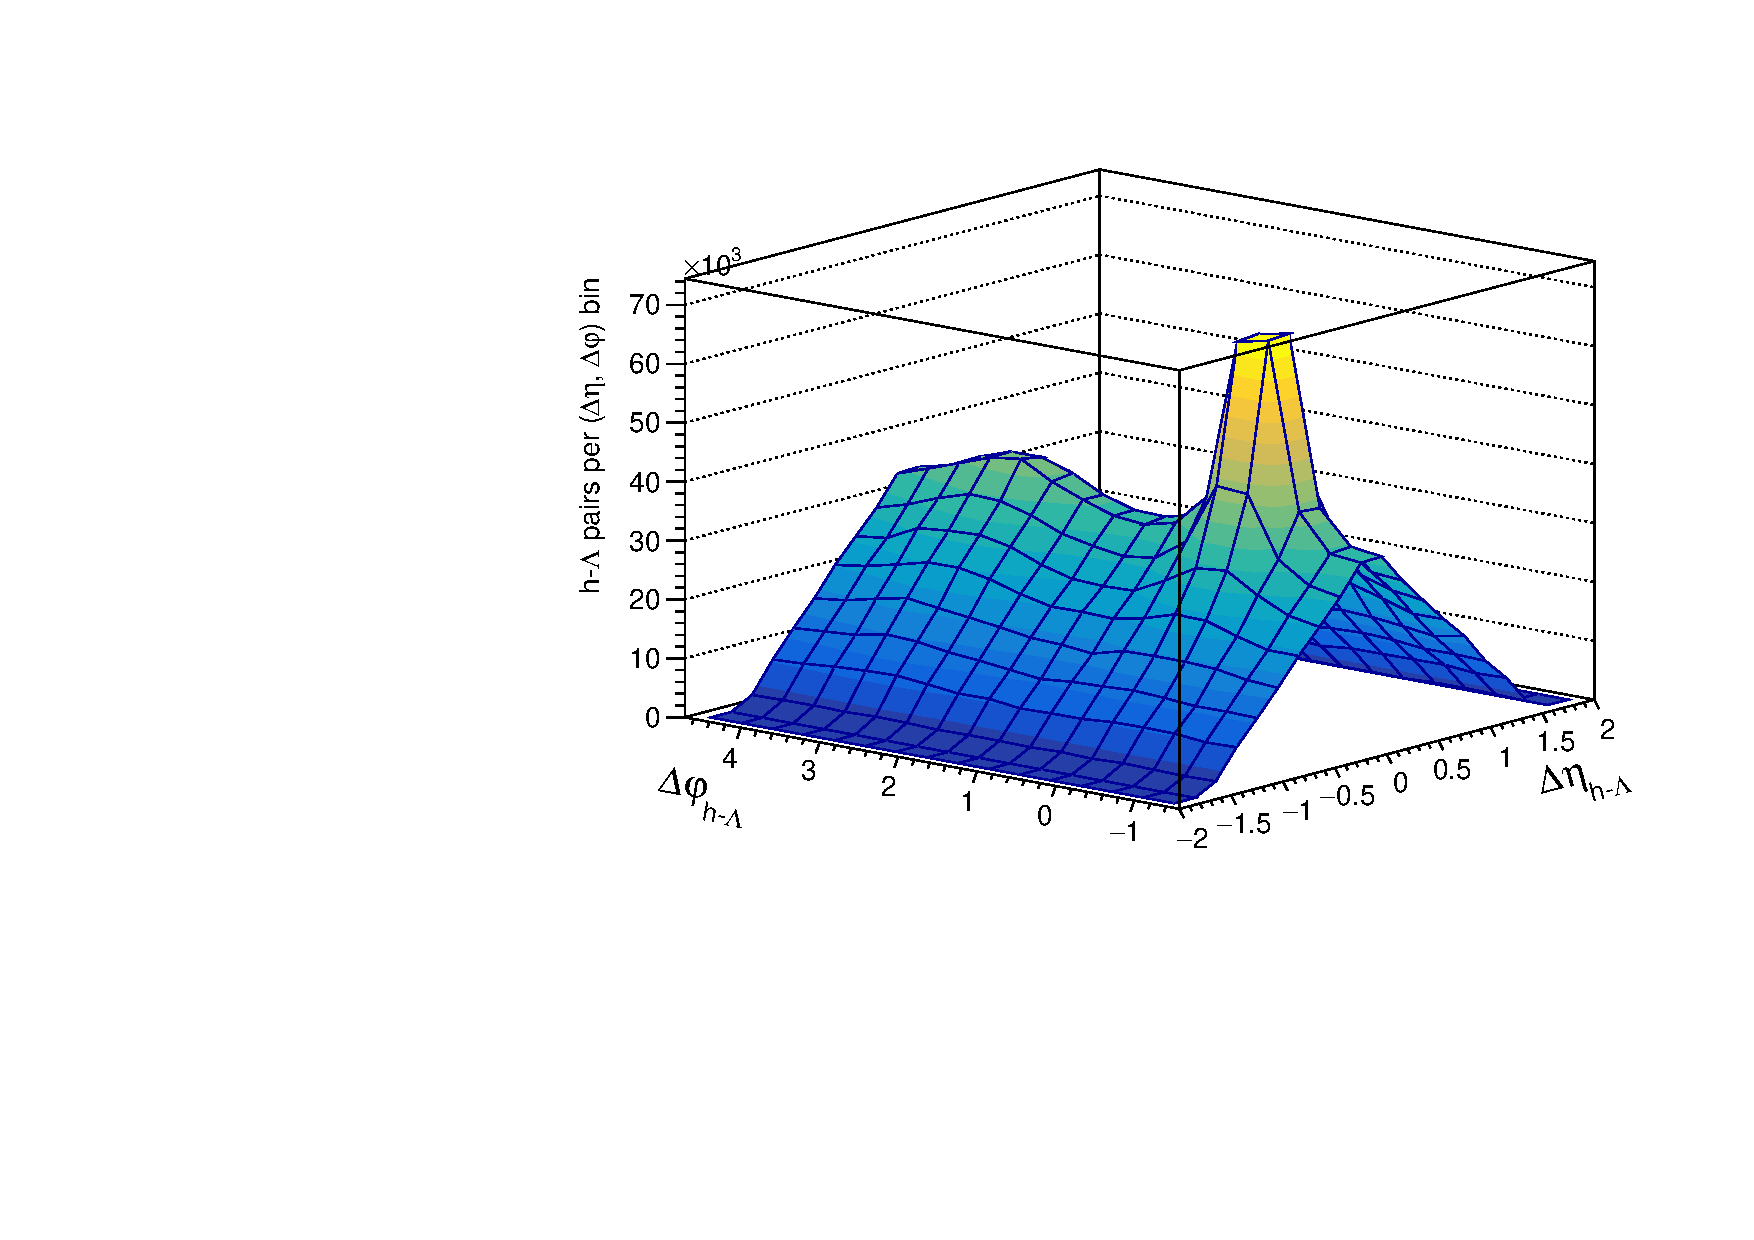
\includegraphics[width=3in]{figures/h_lambda_2d_nomixcor_0_20.pdf}}
\end{subfigure}
\begin{subfigure}{
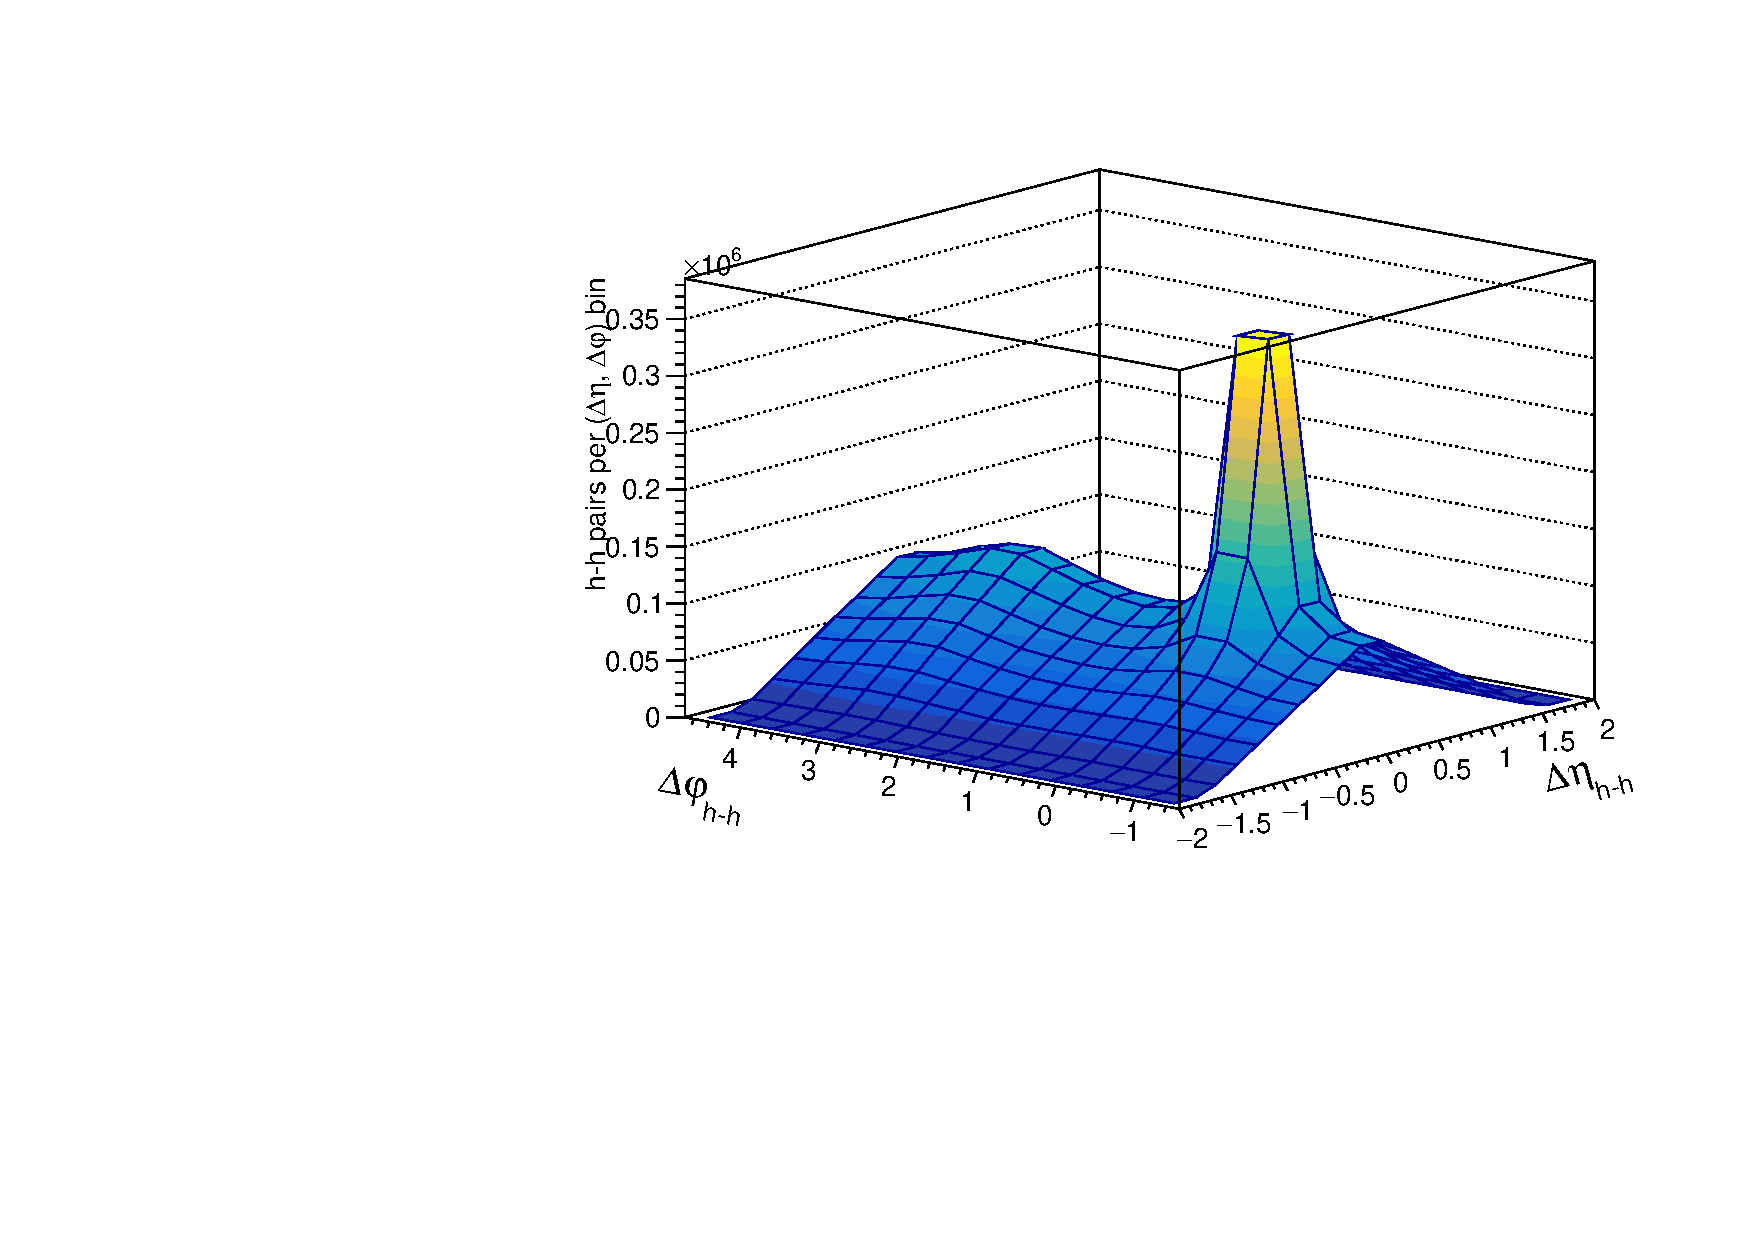
\includegraphics[width=3in]{figures/h_h_2d_nomixcor_0_20.pdf}}
\end{subfigure}
\caption{2-D non-acceptance corrected h-$p\pi$ (left) and h-h (right) angular correlations for the 0-20\% multiplicity bin (all z-vertex bins merged together)}
\label{uncorr2d_0_20}
\end{figure}

\clearpage

\begin{figure}[ht]
\centering
\begin{subfigure}{
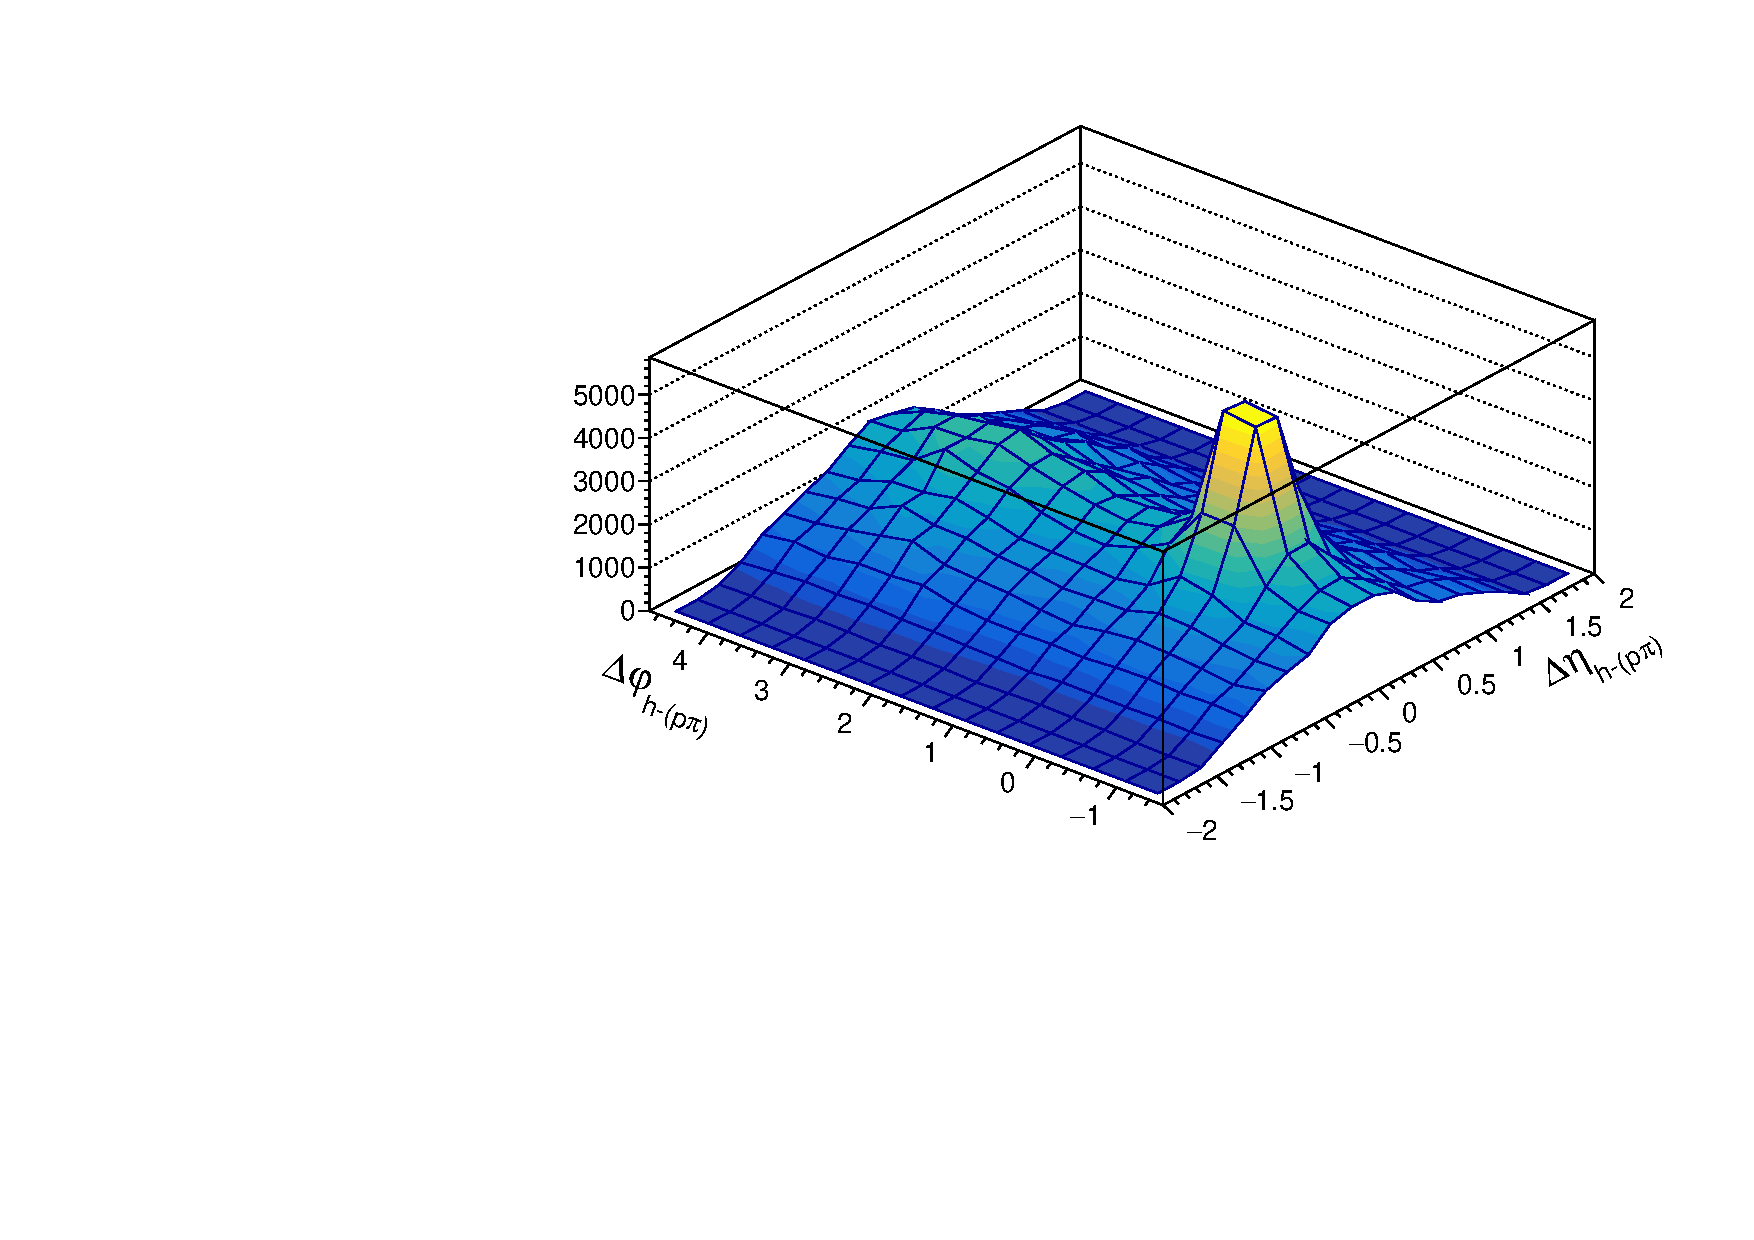
\includegraphics[width=3in]{figures/h_lambda_2d_nomixcor_20_50.pdf}}
\end{subfigure}
\begin{subfigure}{
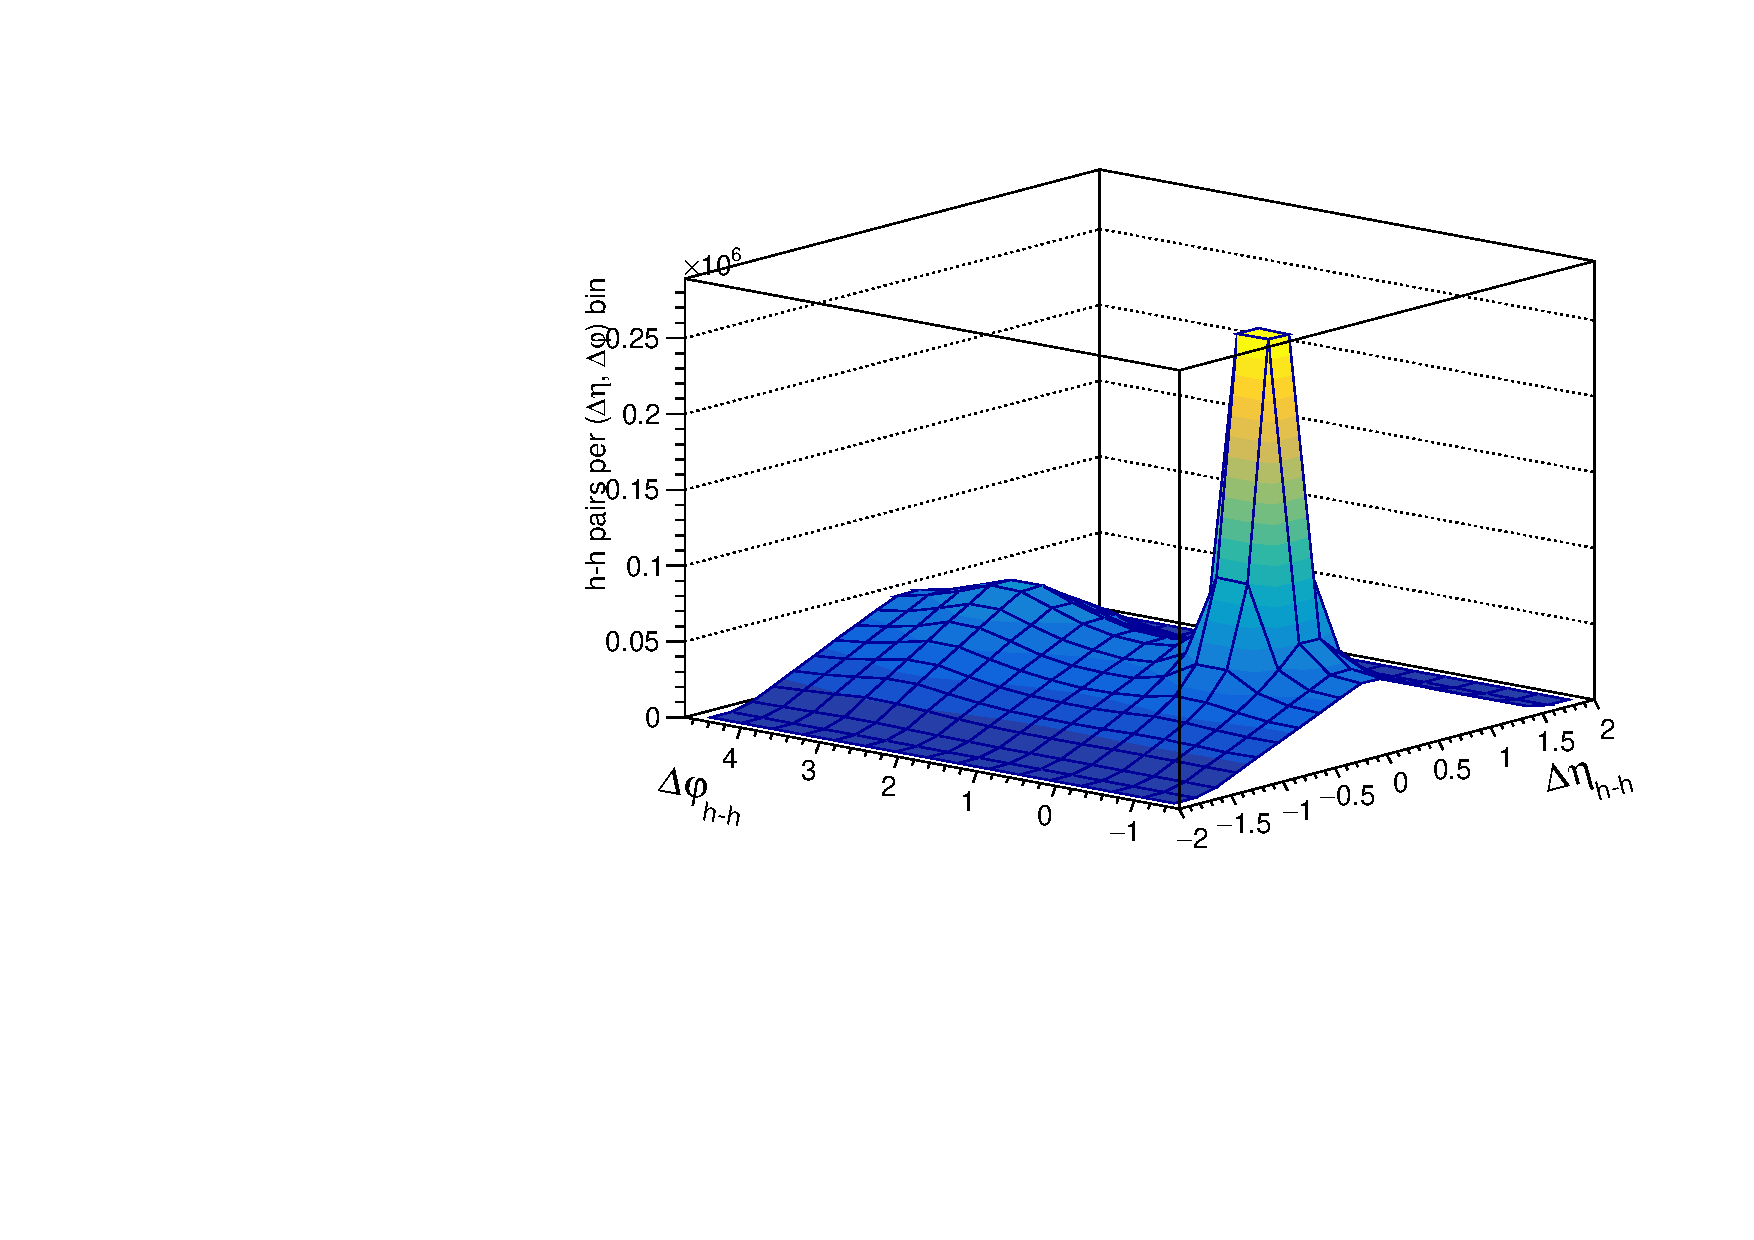
\includegraphics[width=3in]{figures/h_h_2d_nomixcor_20_50.pdf}}
\end{subfigure}
\caption{2-D non-acceptance corrected h-$p\pi$ (left) and h-h (right) angular correlations for the 20-50\% multiplicity bin (all z-vertex bins merged together)}
\label{uncorr2d_20_50}
\end{figure}

\begin{figure}[ht]
\centering
\begin{subfigure}{
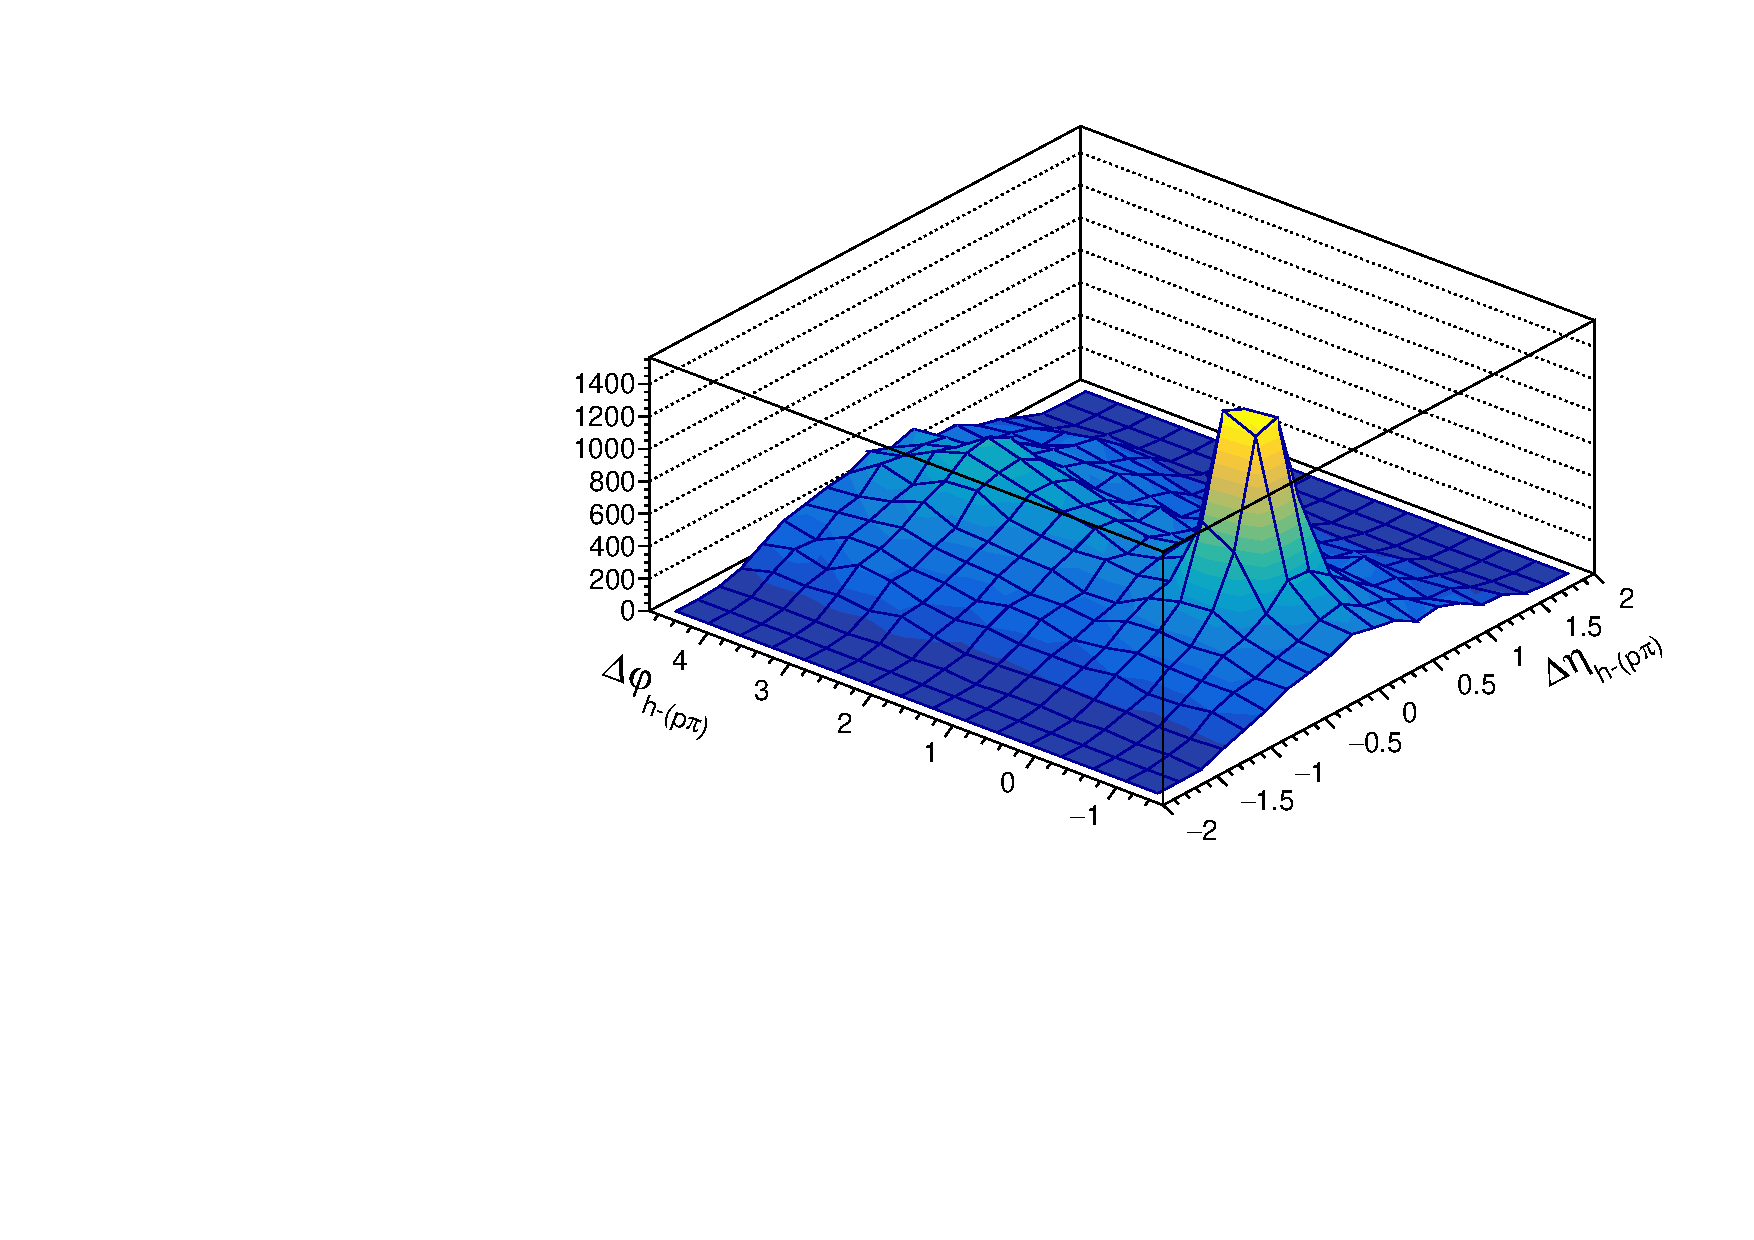
\includegraphics[width=3in]{figures/h_lambda_2d_nomixcor_50_80.pdf}}
\end{subfigure}
\begin{subfigure}{
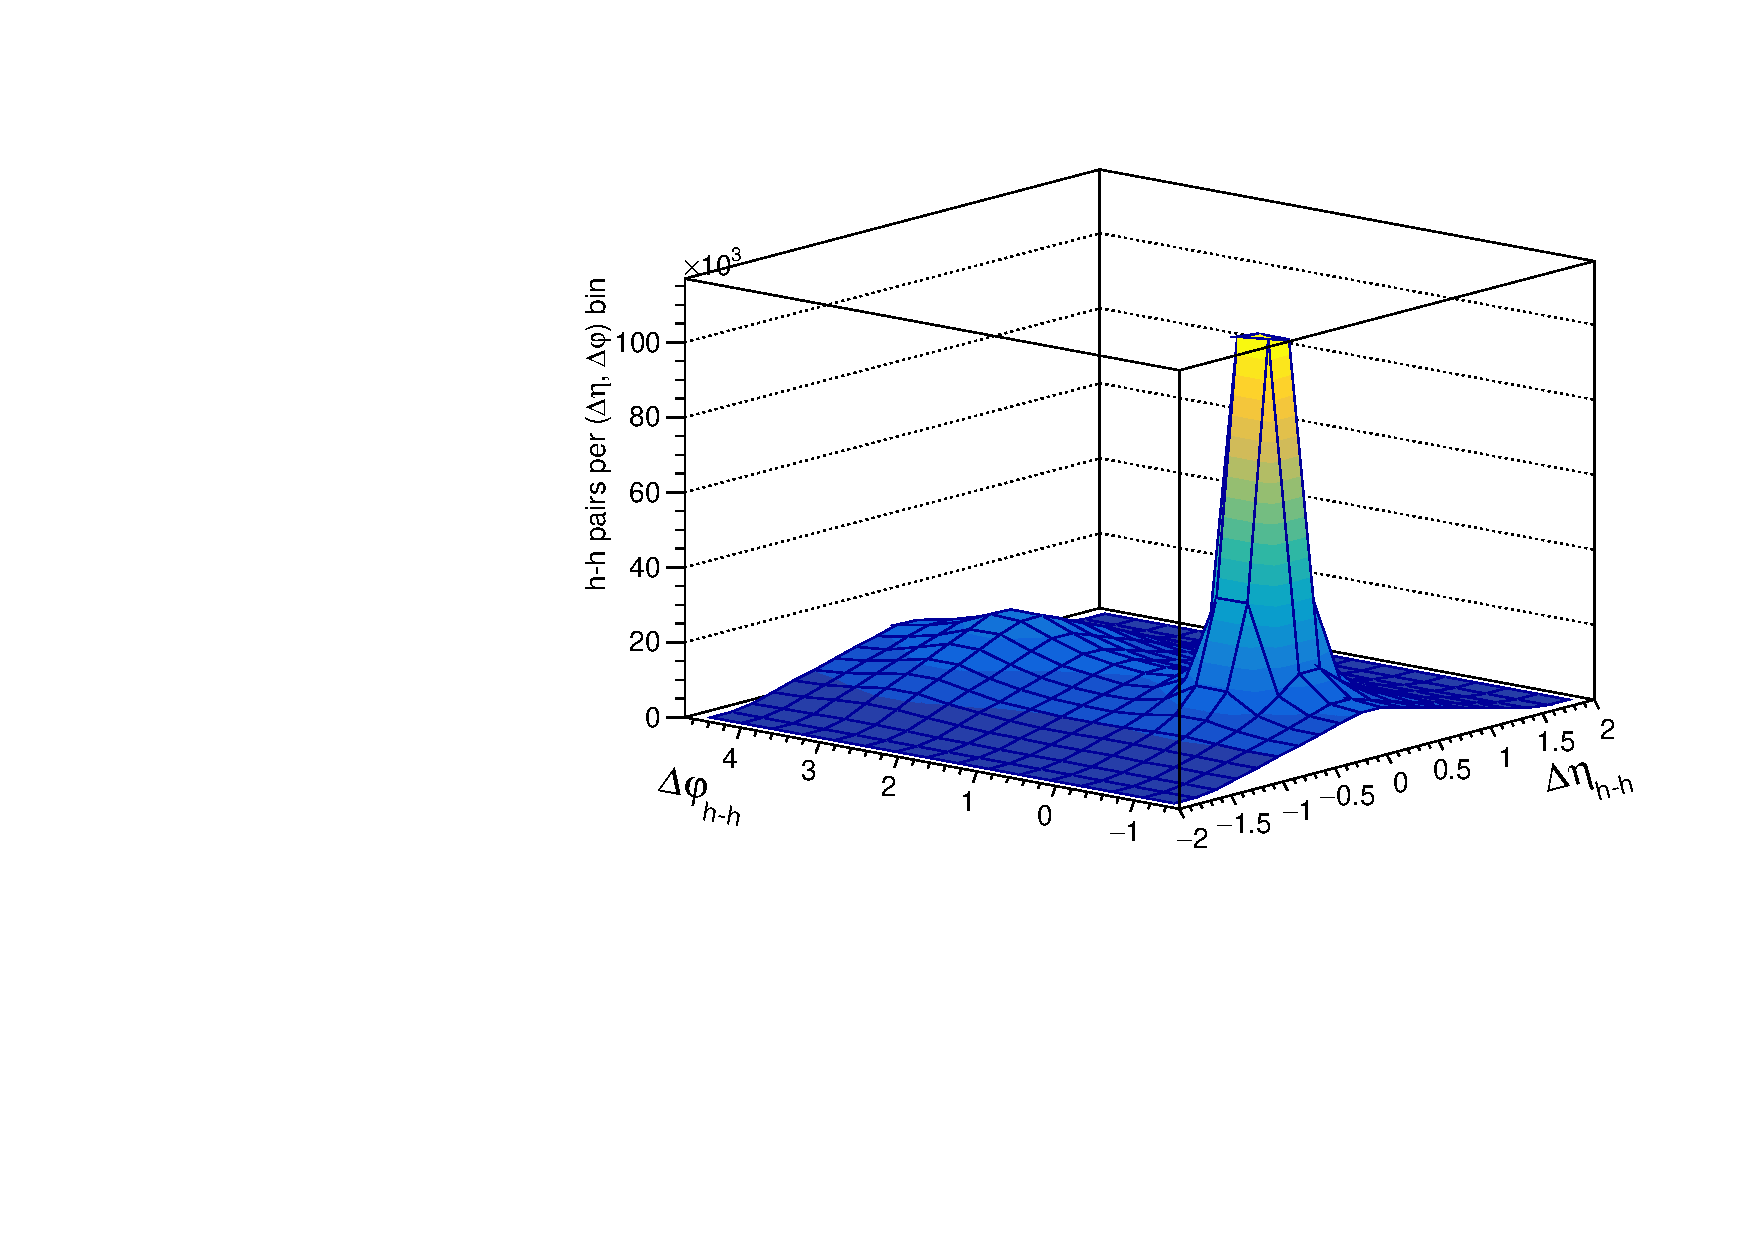
\includegraphics[width=3in]{figures/h_h_2d_nomixcor_50_80.pdf}}
\end{subfigure}
\caption{2-D non-acceptance corrected h-$p\pi$ (left) and h-h (right) angular correlations for the 50-80\% multiplicity bin (all z-vertex bins merged together)}
\label{uncorr2d_50_80}
\end{figure}

\begin{figure}[ht]
\centering
\begin{subfigure}{
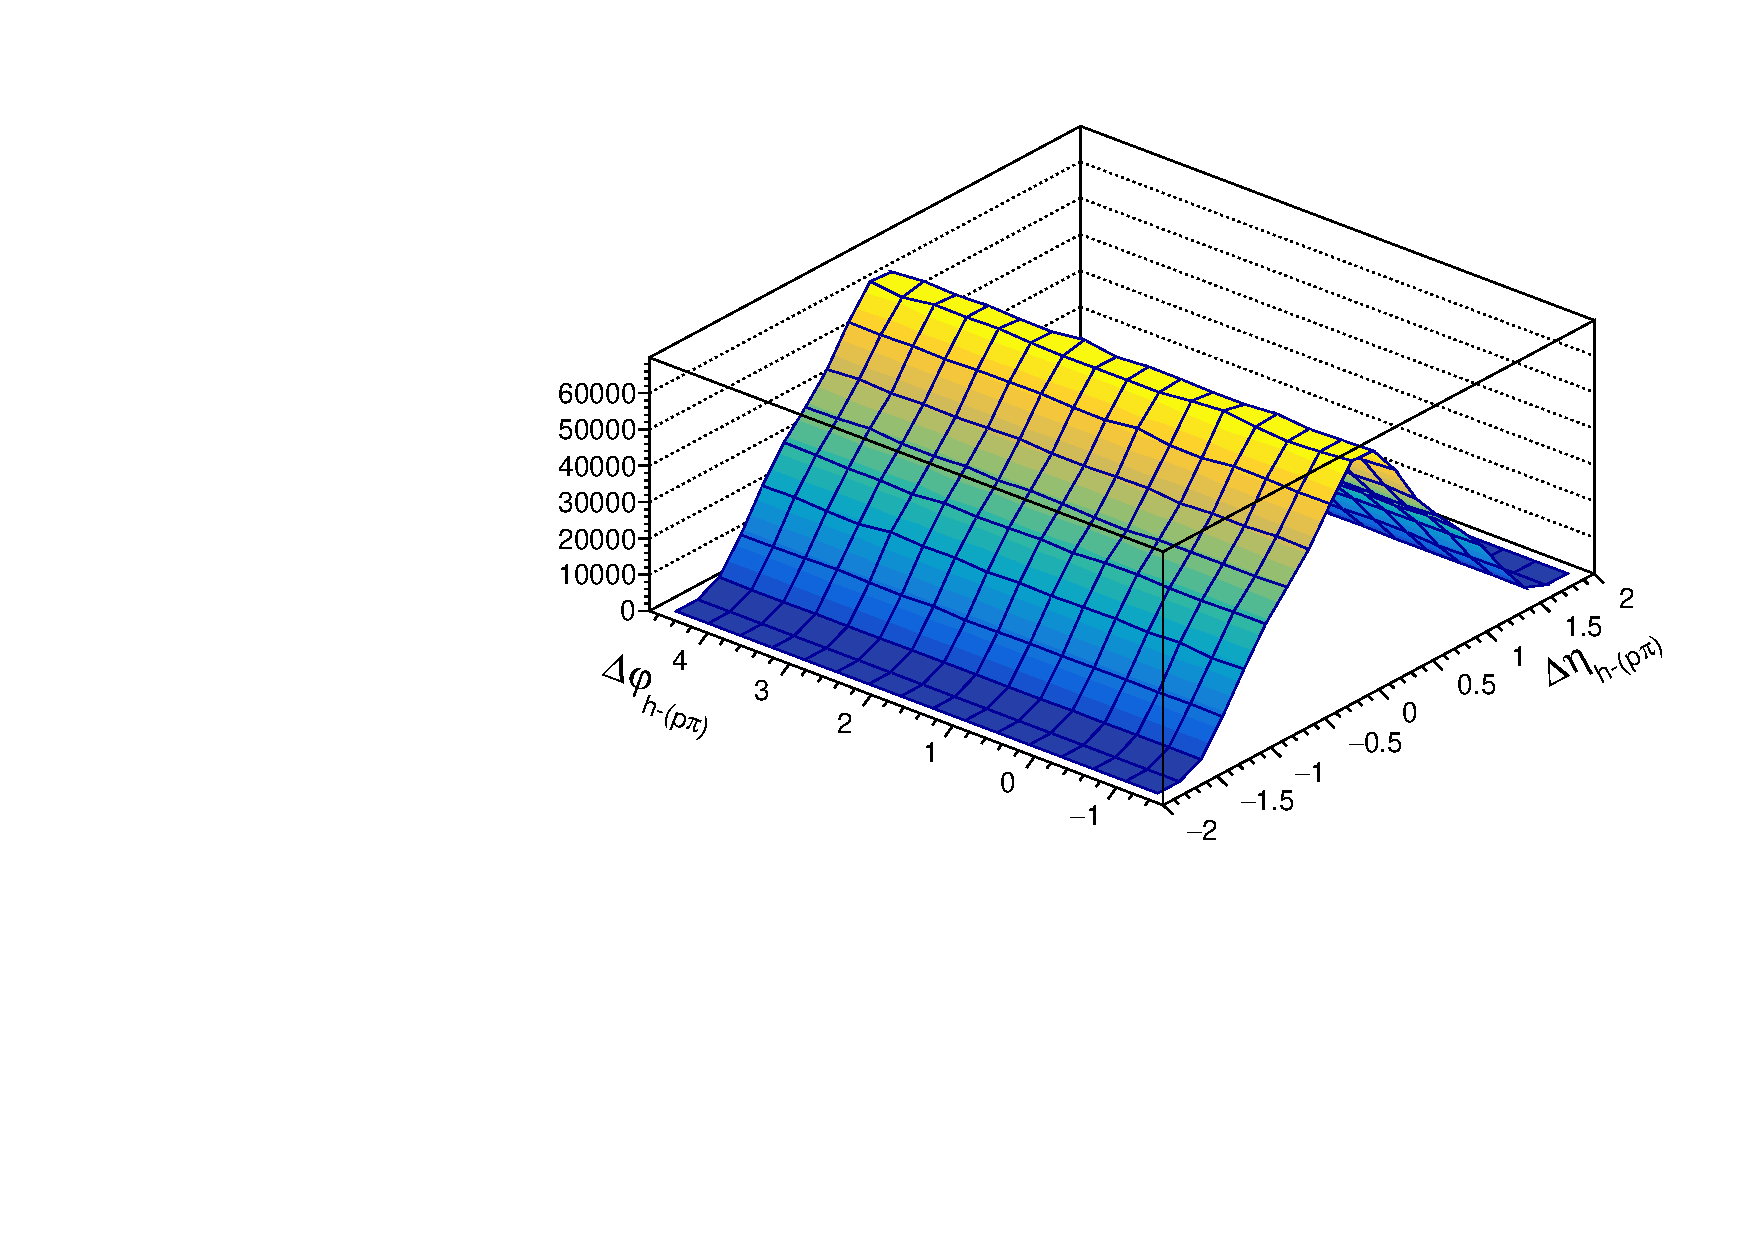
\includegraphics[width=3in]{figures/h_lambda_2d_mixed_0_20.pdf}}
\end{subfigure}
\begin{subfigure}{
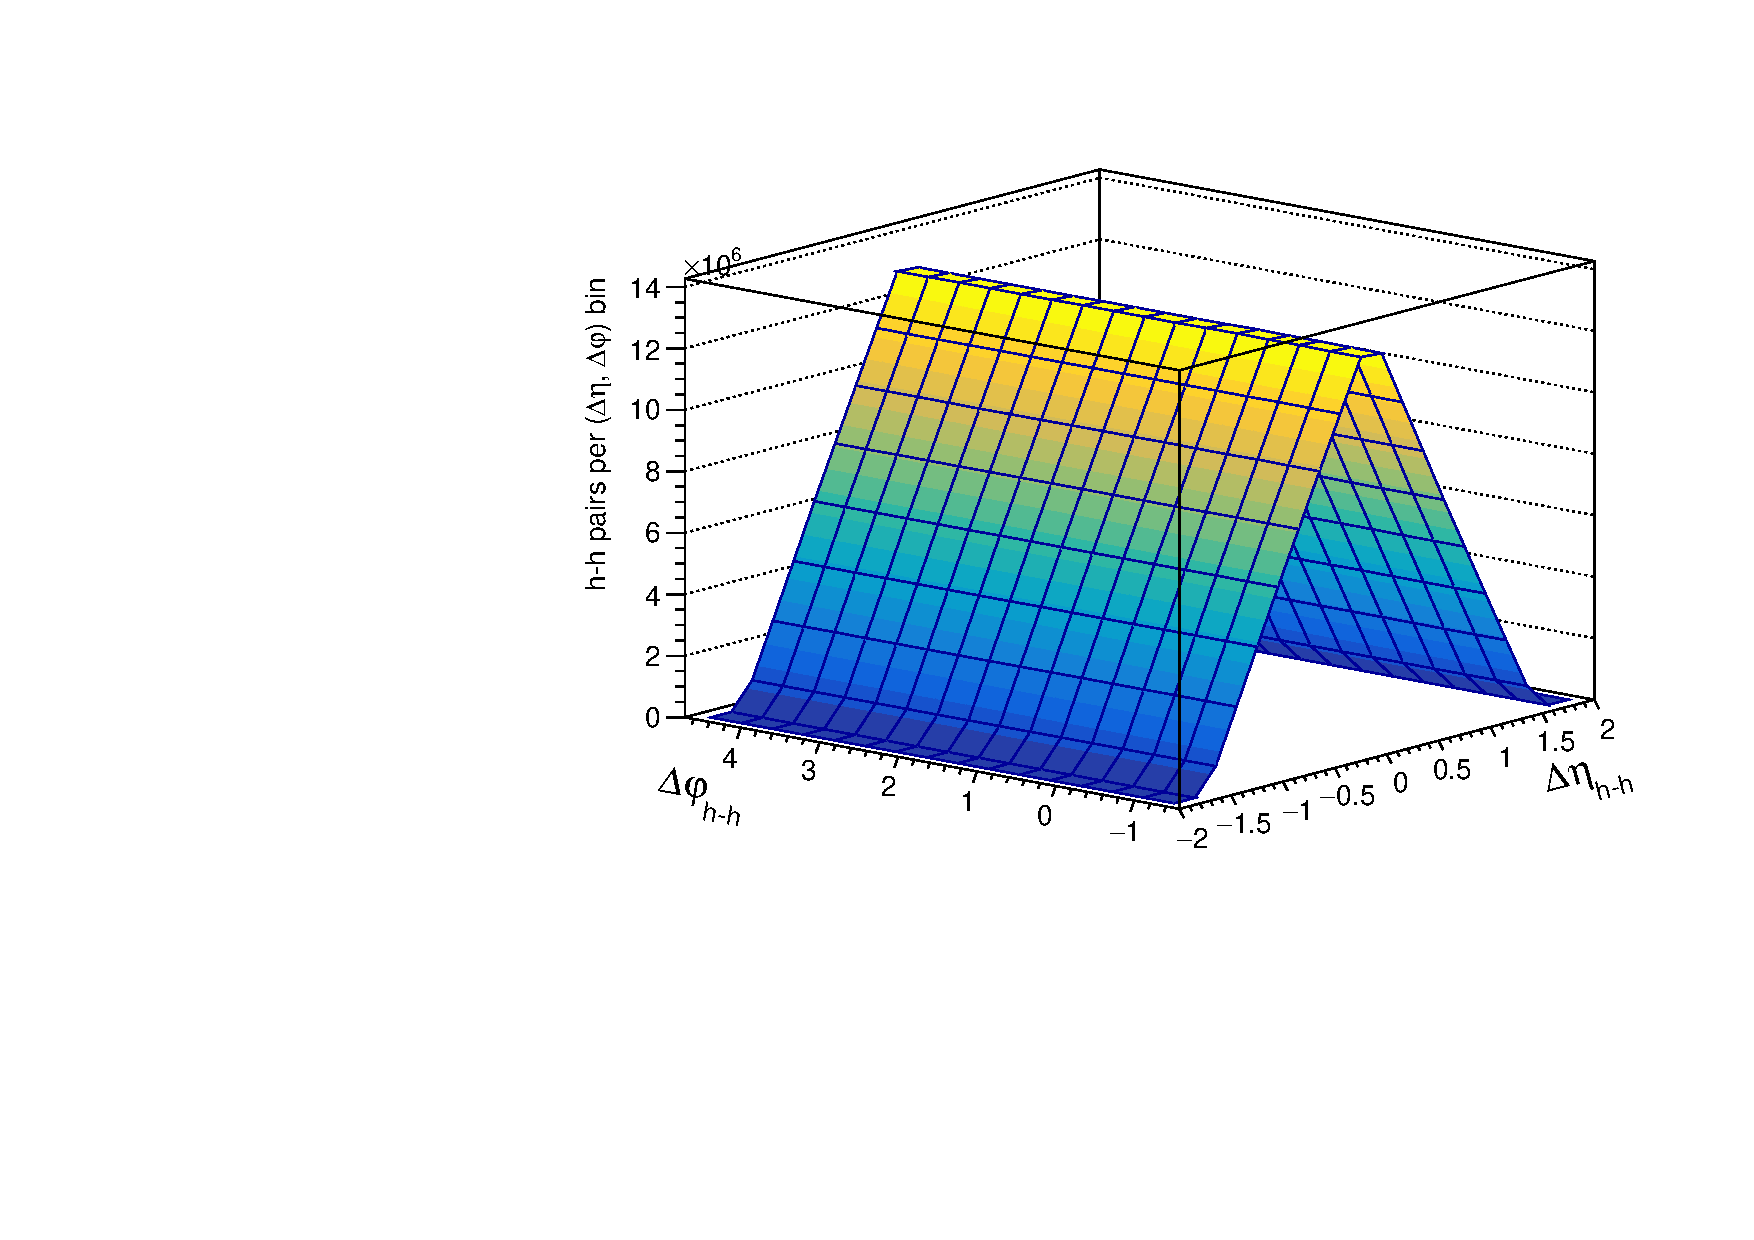
\includegraphics[width=3in]{figures/h_h_2d_mixed_0_20.pdf}}
\end{subfigure}
\caption{2-D mixed event h-$p\pi$ (left) and h-h (right) angular correlations for the 0-20\% multiplicity bin (all z-vertex bins merged together)}
\label{mixed2d_0_20}
\end{figure}

\begin{figure}[ht]
\centering
\begin{subfigure}{
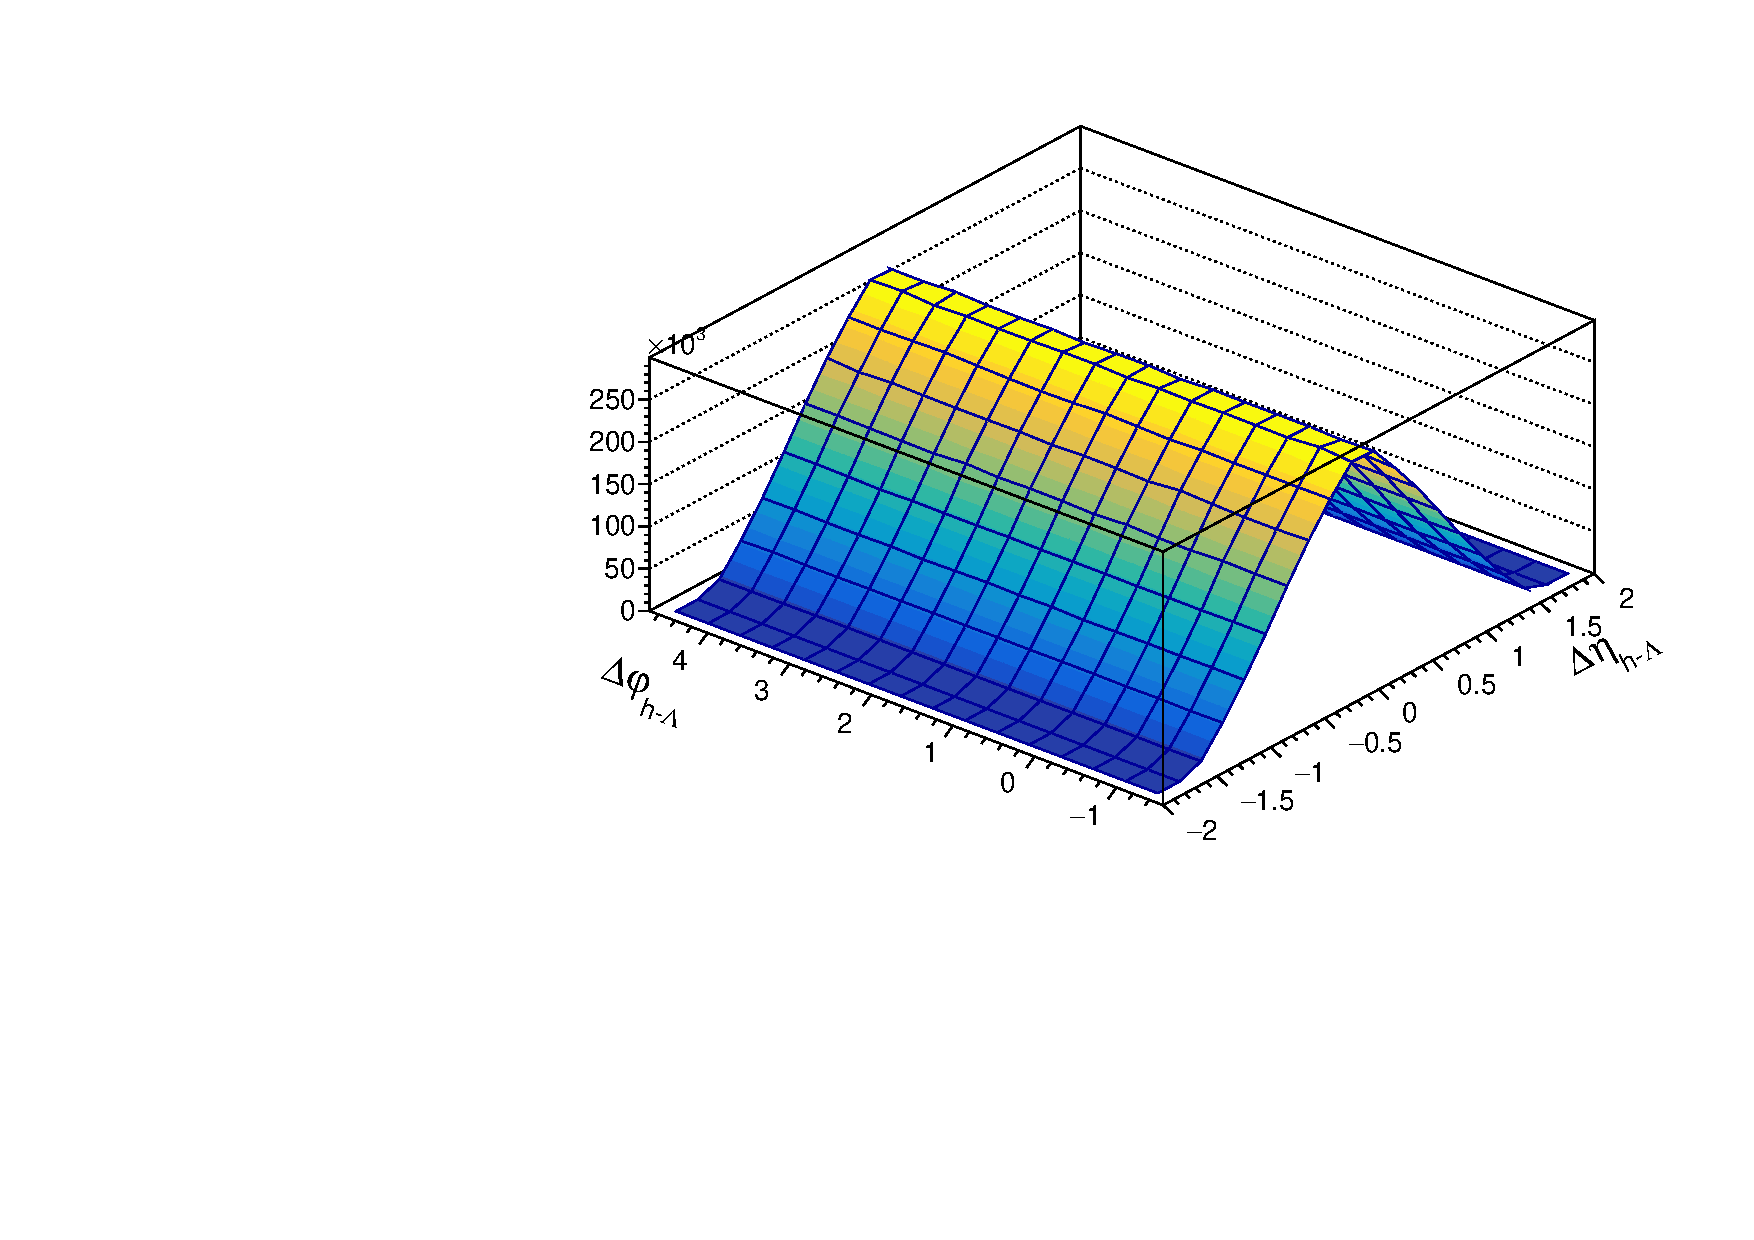
\includegraphics[width=3in]{figures/h_lambda_2d_mixed_20_50.pdf}}
\end{subfigure}
\begin{subfigure}{
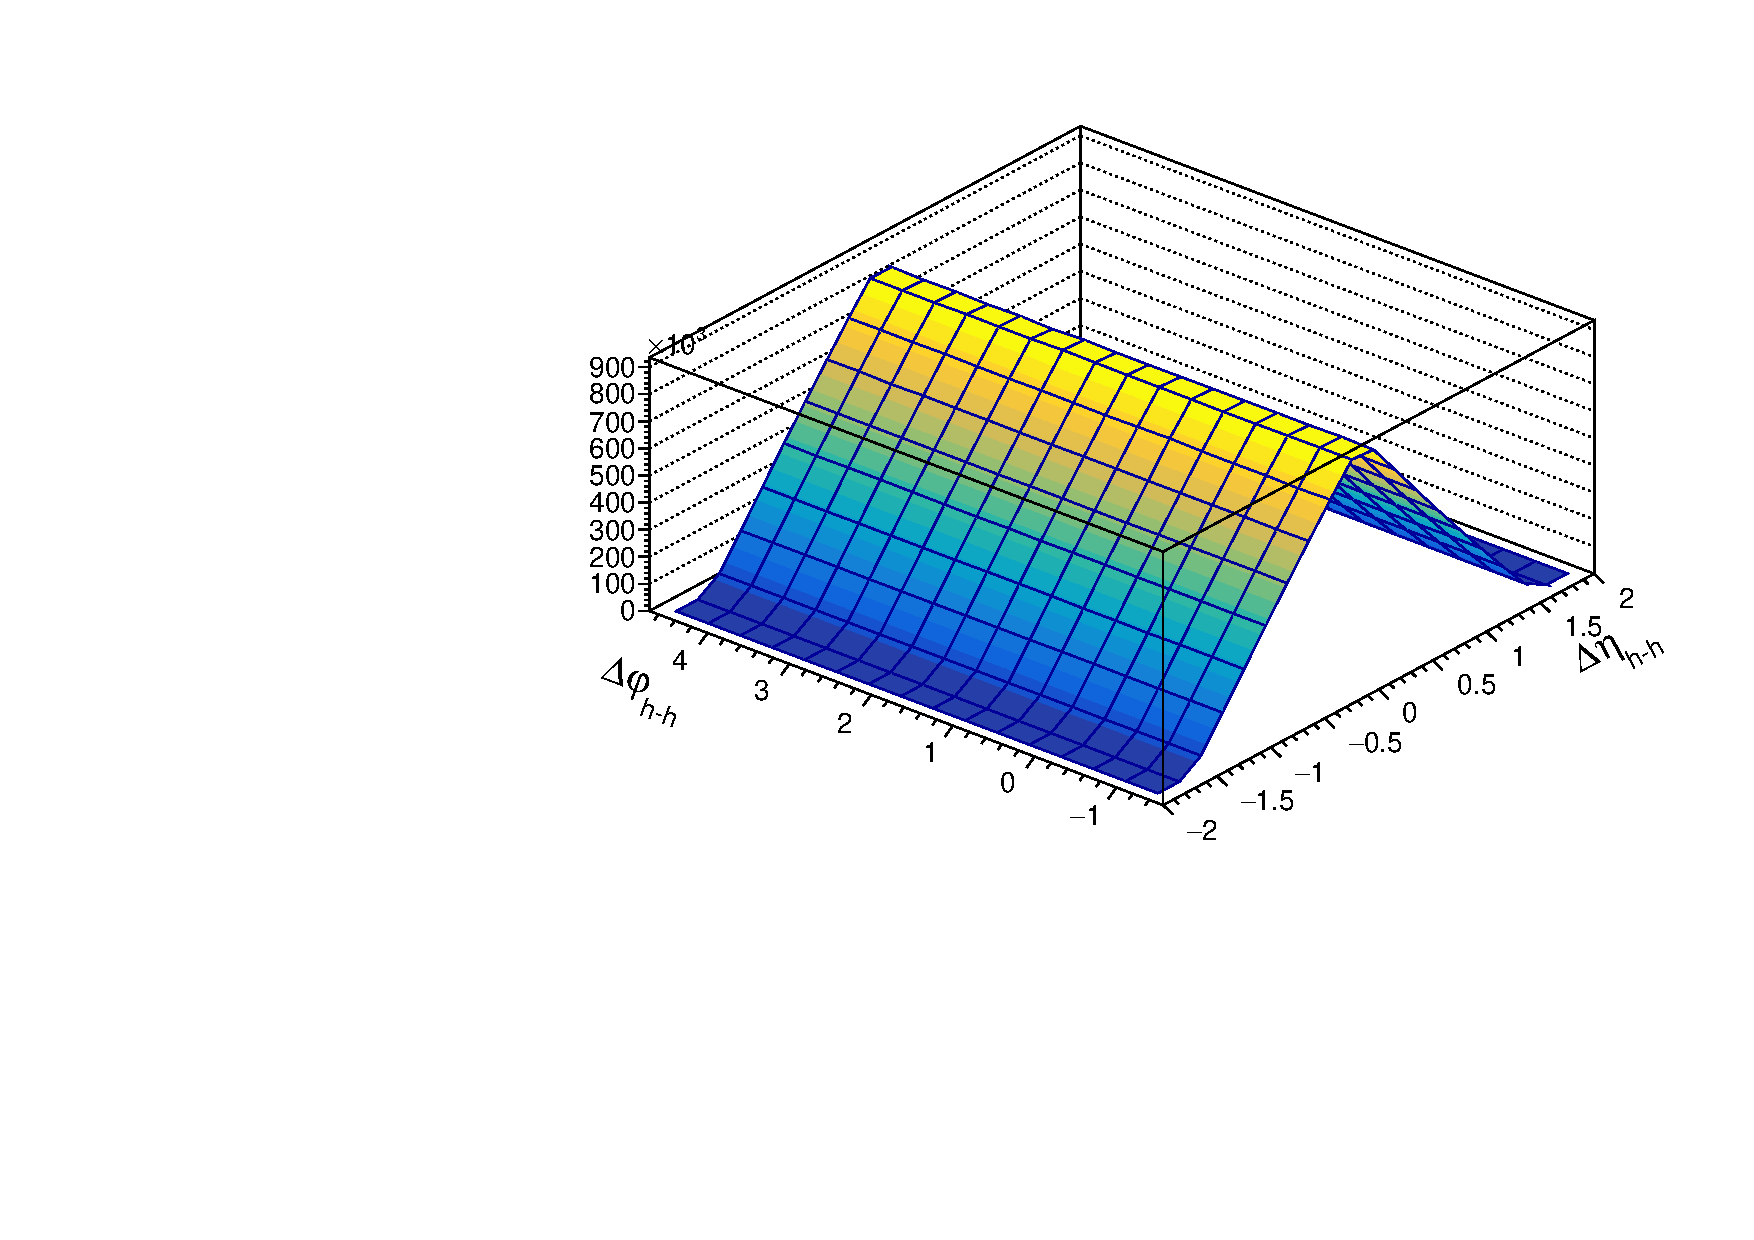
\includegraphics[width=3in]{figures/h_h_2d_mixed_20_50.pdf}}
\end{subfigure}
\caption{2-D mixed event h-$p\pi$ (left) and h-h (right) angular correlations for the 20-50\% multiplicity bin (all z-vertex bins merged together)}
\label{mixed2d_20_50}
\end{figure}

\begin{figure}[ht]
\centering
\begin{subfigure}{
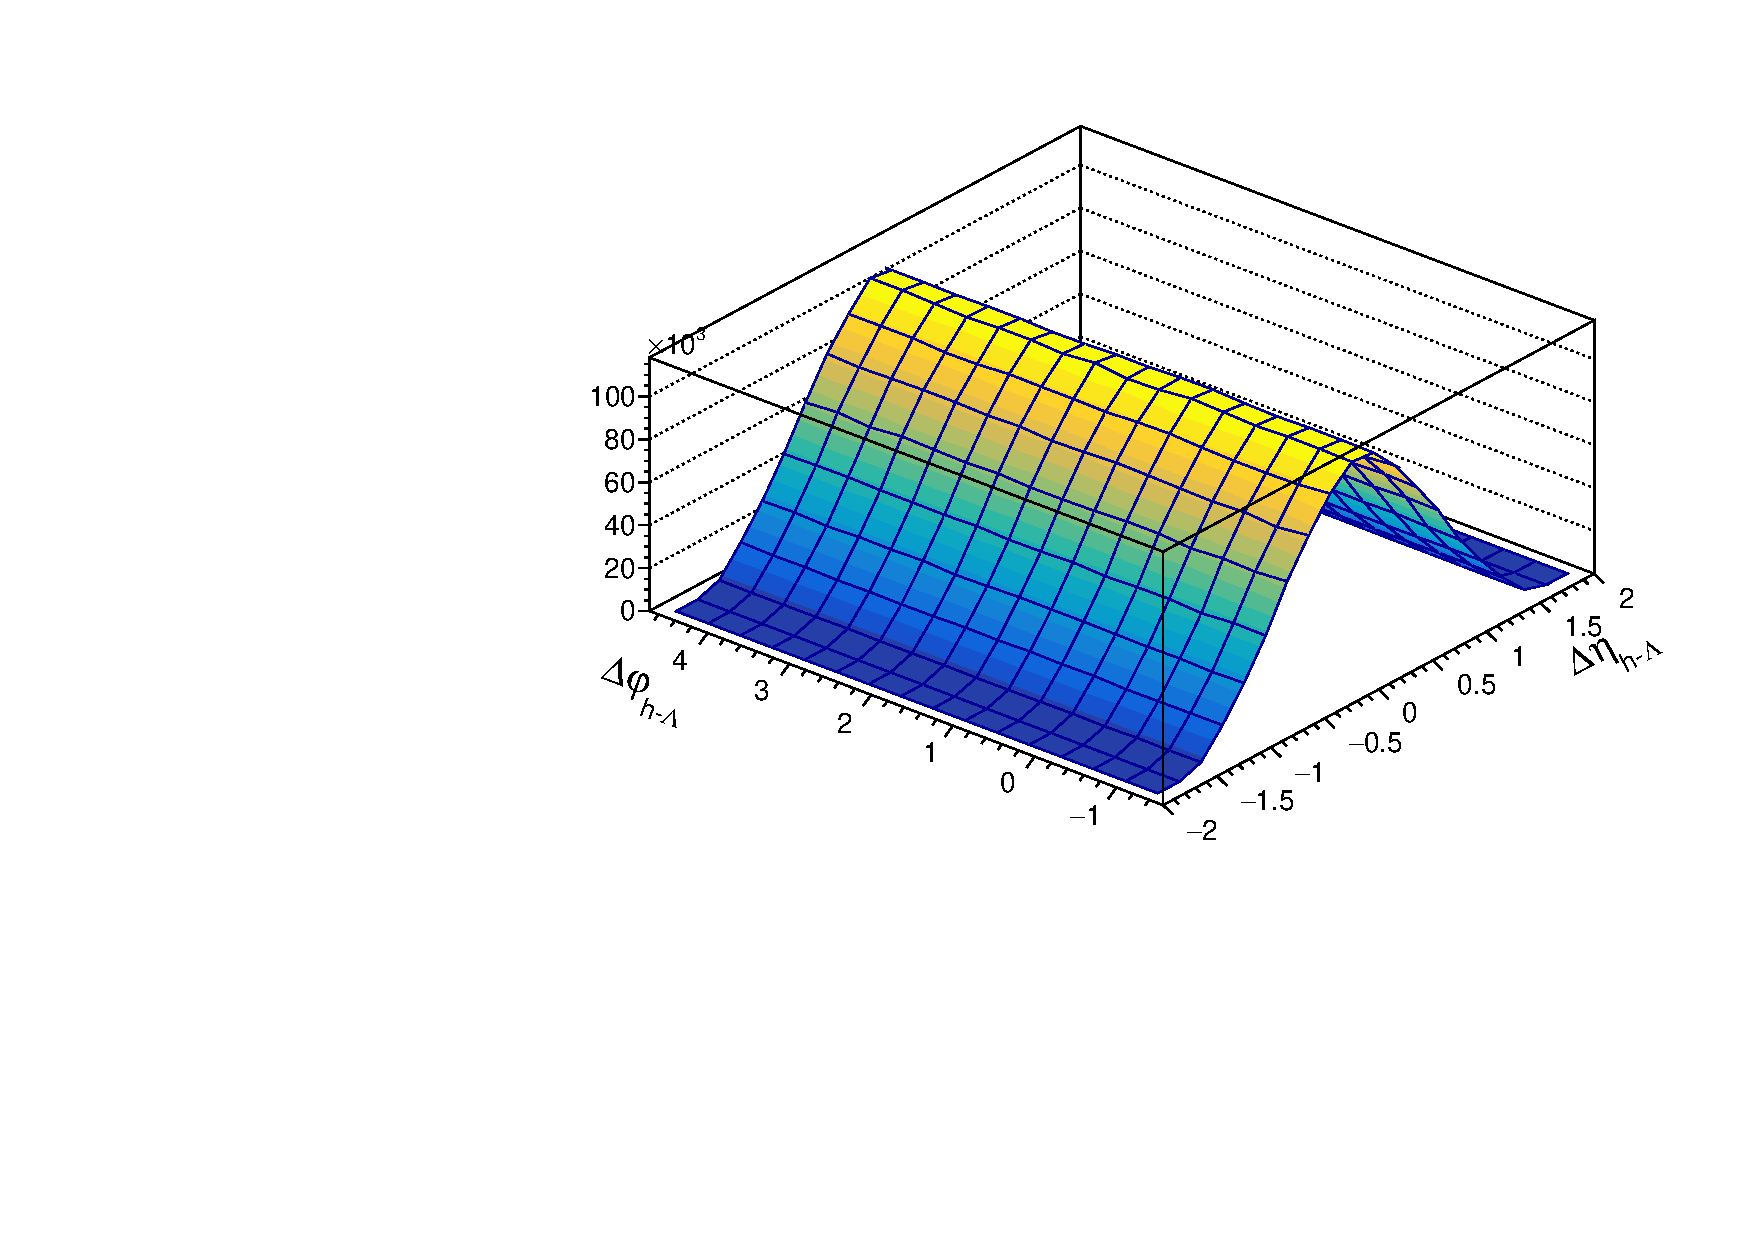
\includegraphics[width=3in]{figures/h_lambda_2d_mixed_50_80.pdf}}
\end{subfigure}
\begin{subfigure}{
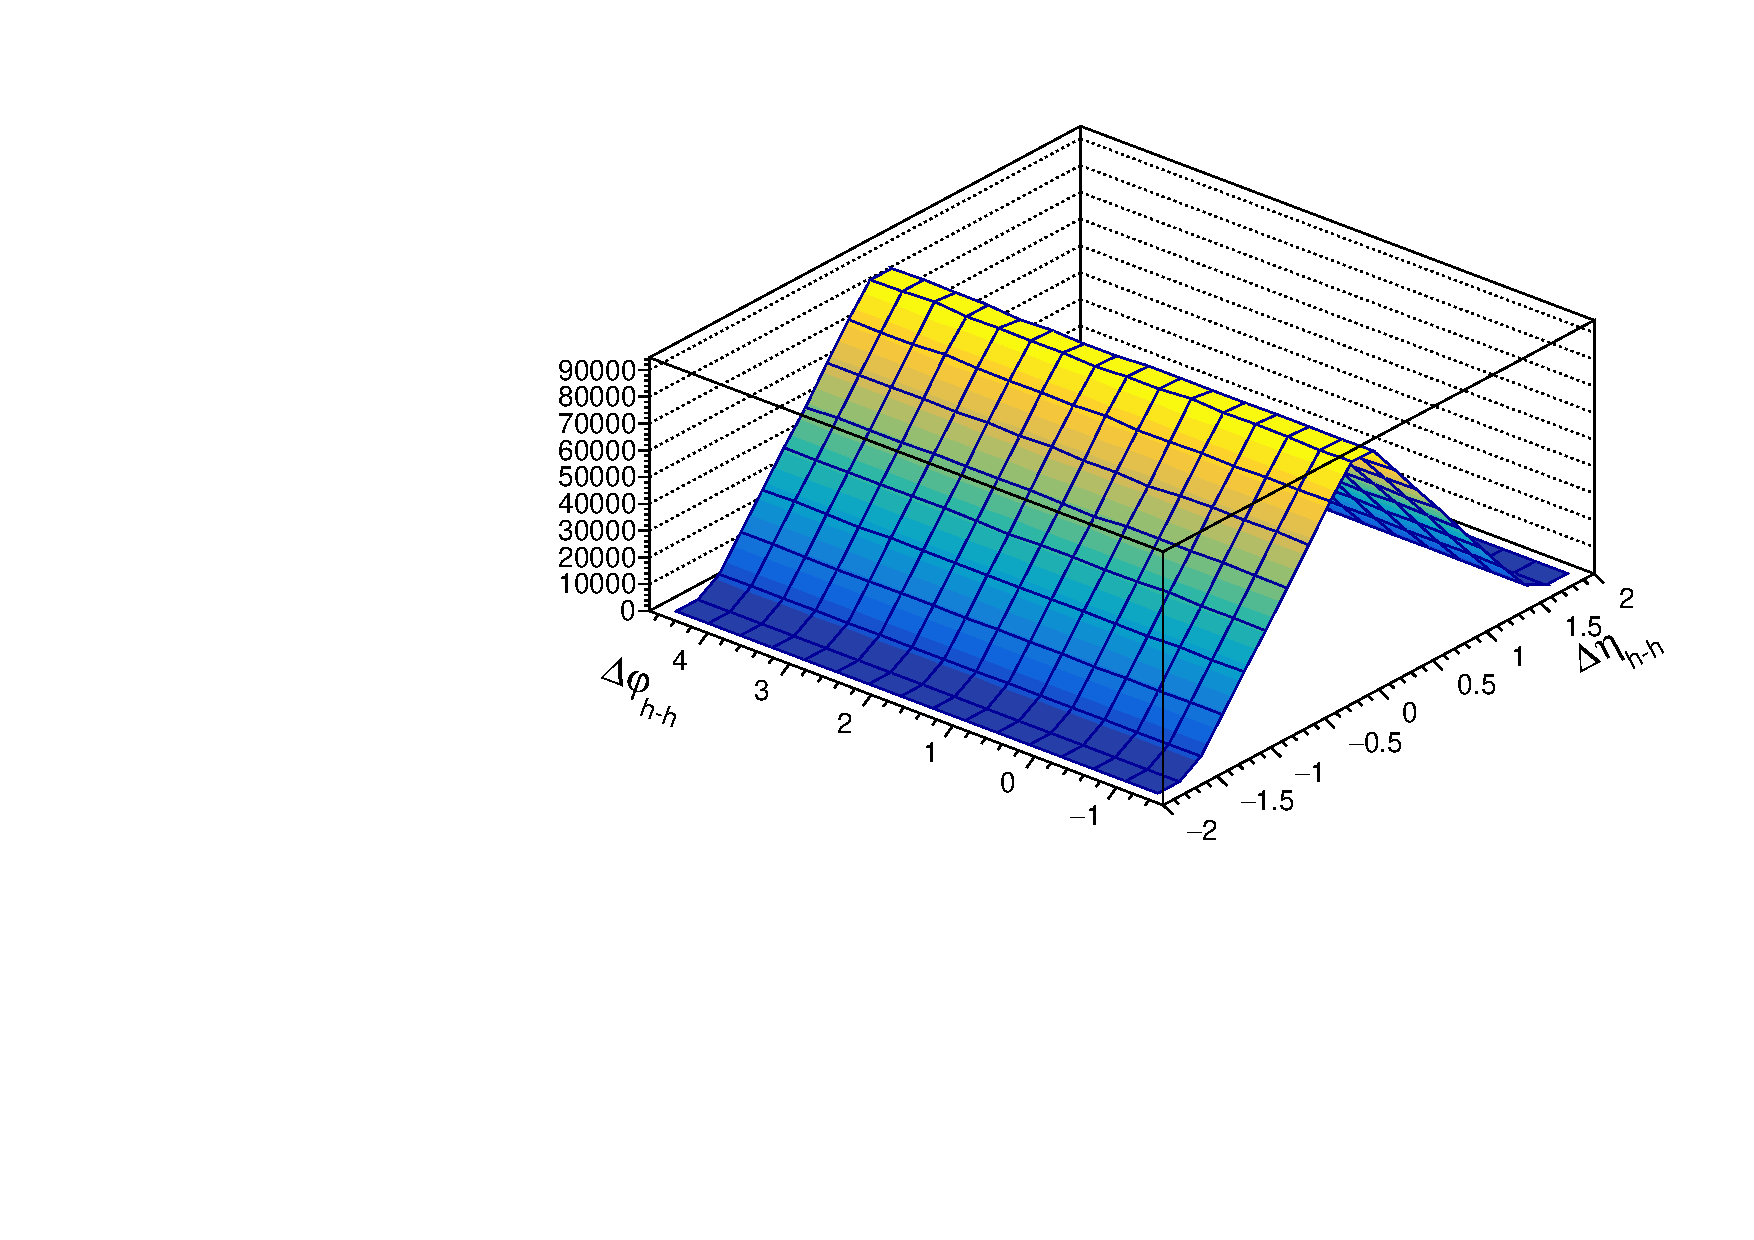
\includegraphics[width=3in]{figures/h_h_2d_mixed_50_80.pdf}}
\end{subfigure}
\caption{2-D mixed event h-$p\pi$ (left) and h-h (right) angular correlations for the 50-80\% multiplicity bin (all z-vertex bins merged together)}
\label{mixed2d_50_80}
\end{figure}


\begin{figure}[ht]
\centering
\begin{subfigure}{
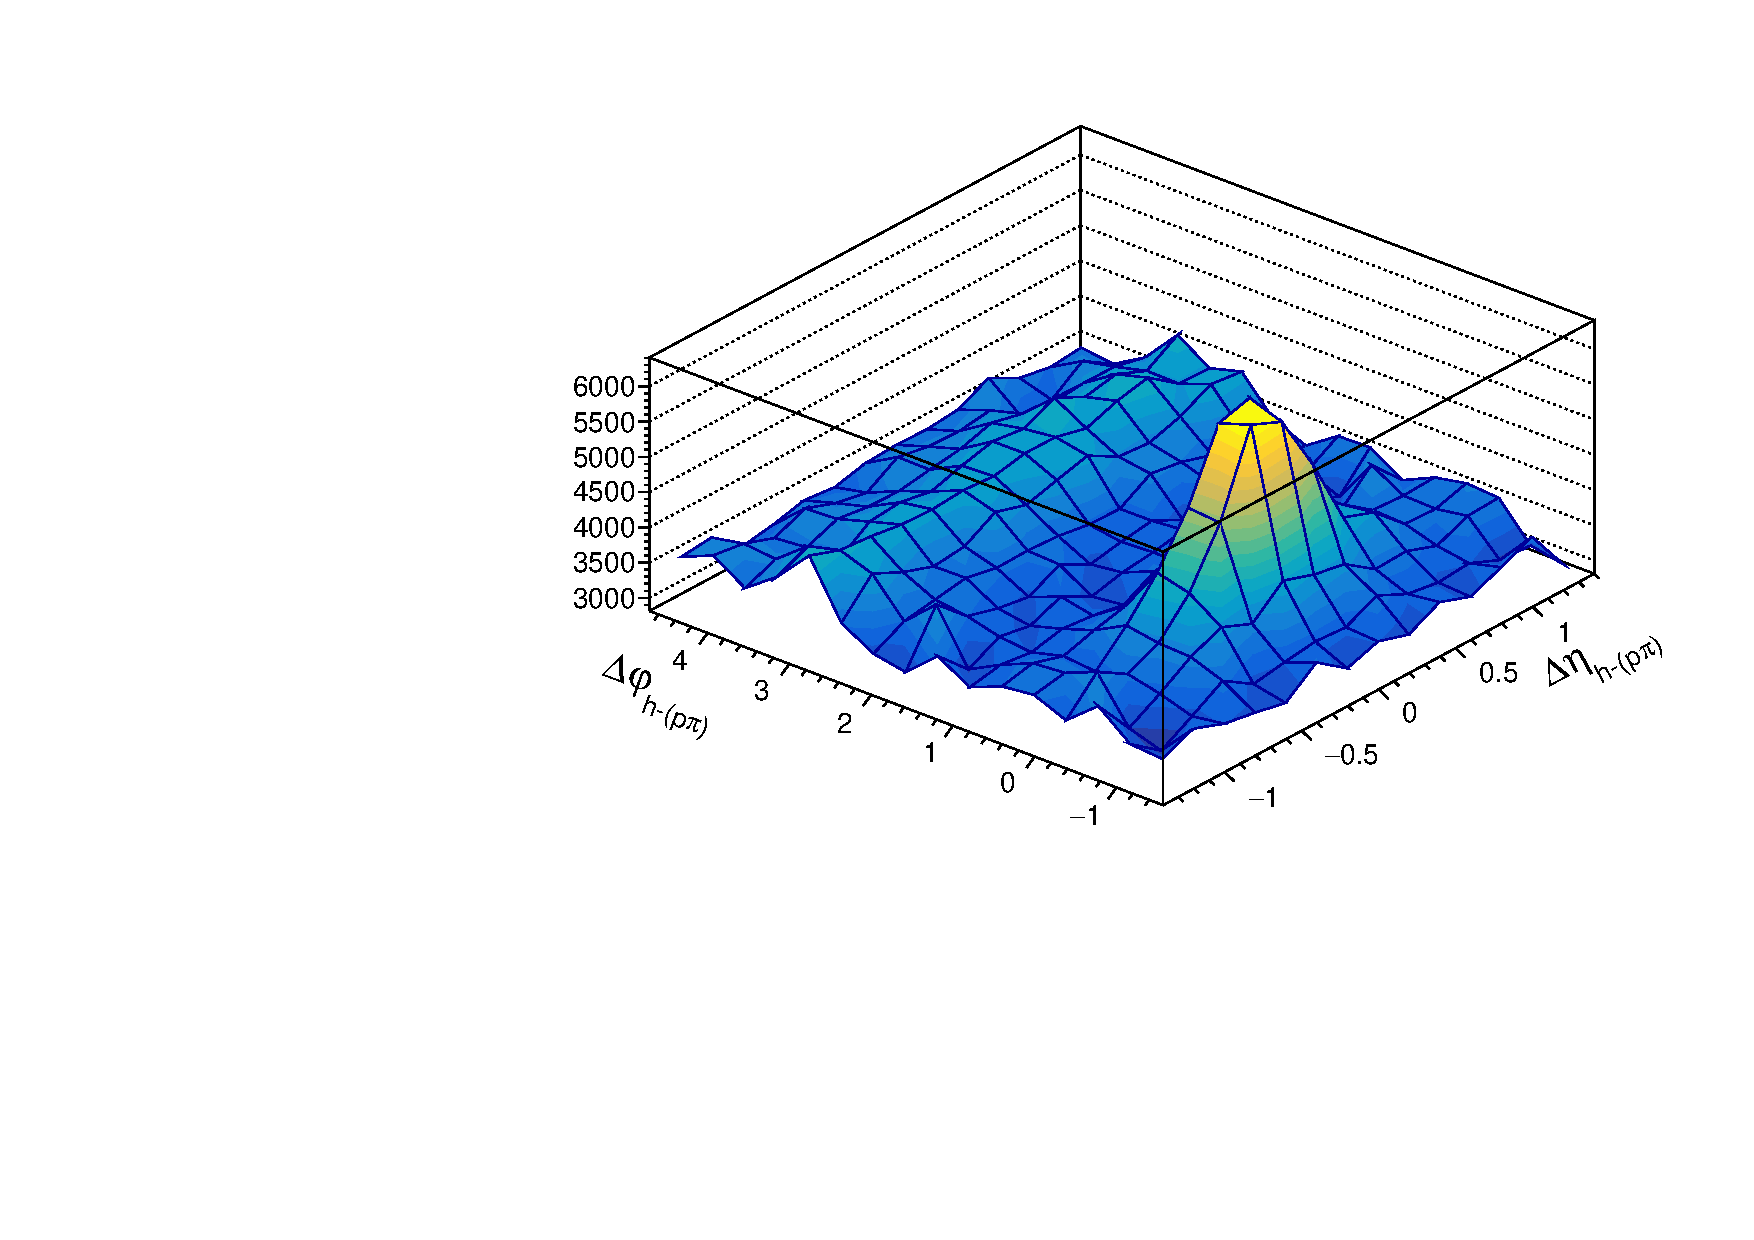
\includegraphics[width=3in]{figures/h_lambda_2d_mixcor_0_20.pdf}}
\end{subfigure}
\begin{subfigure}{
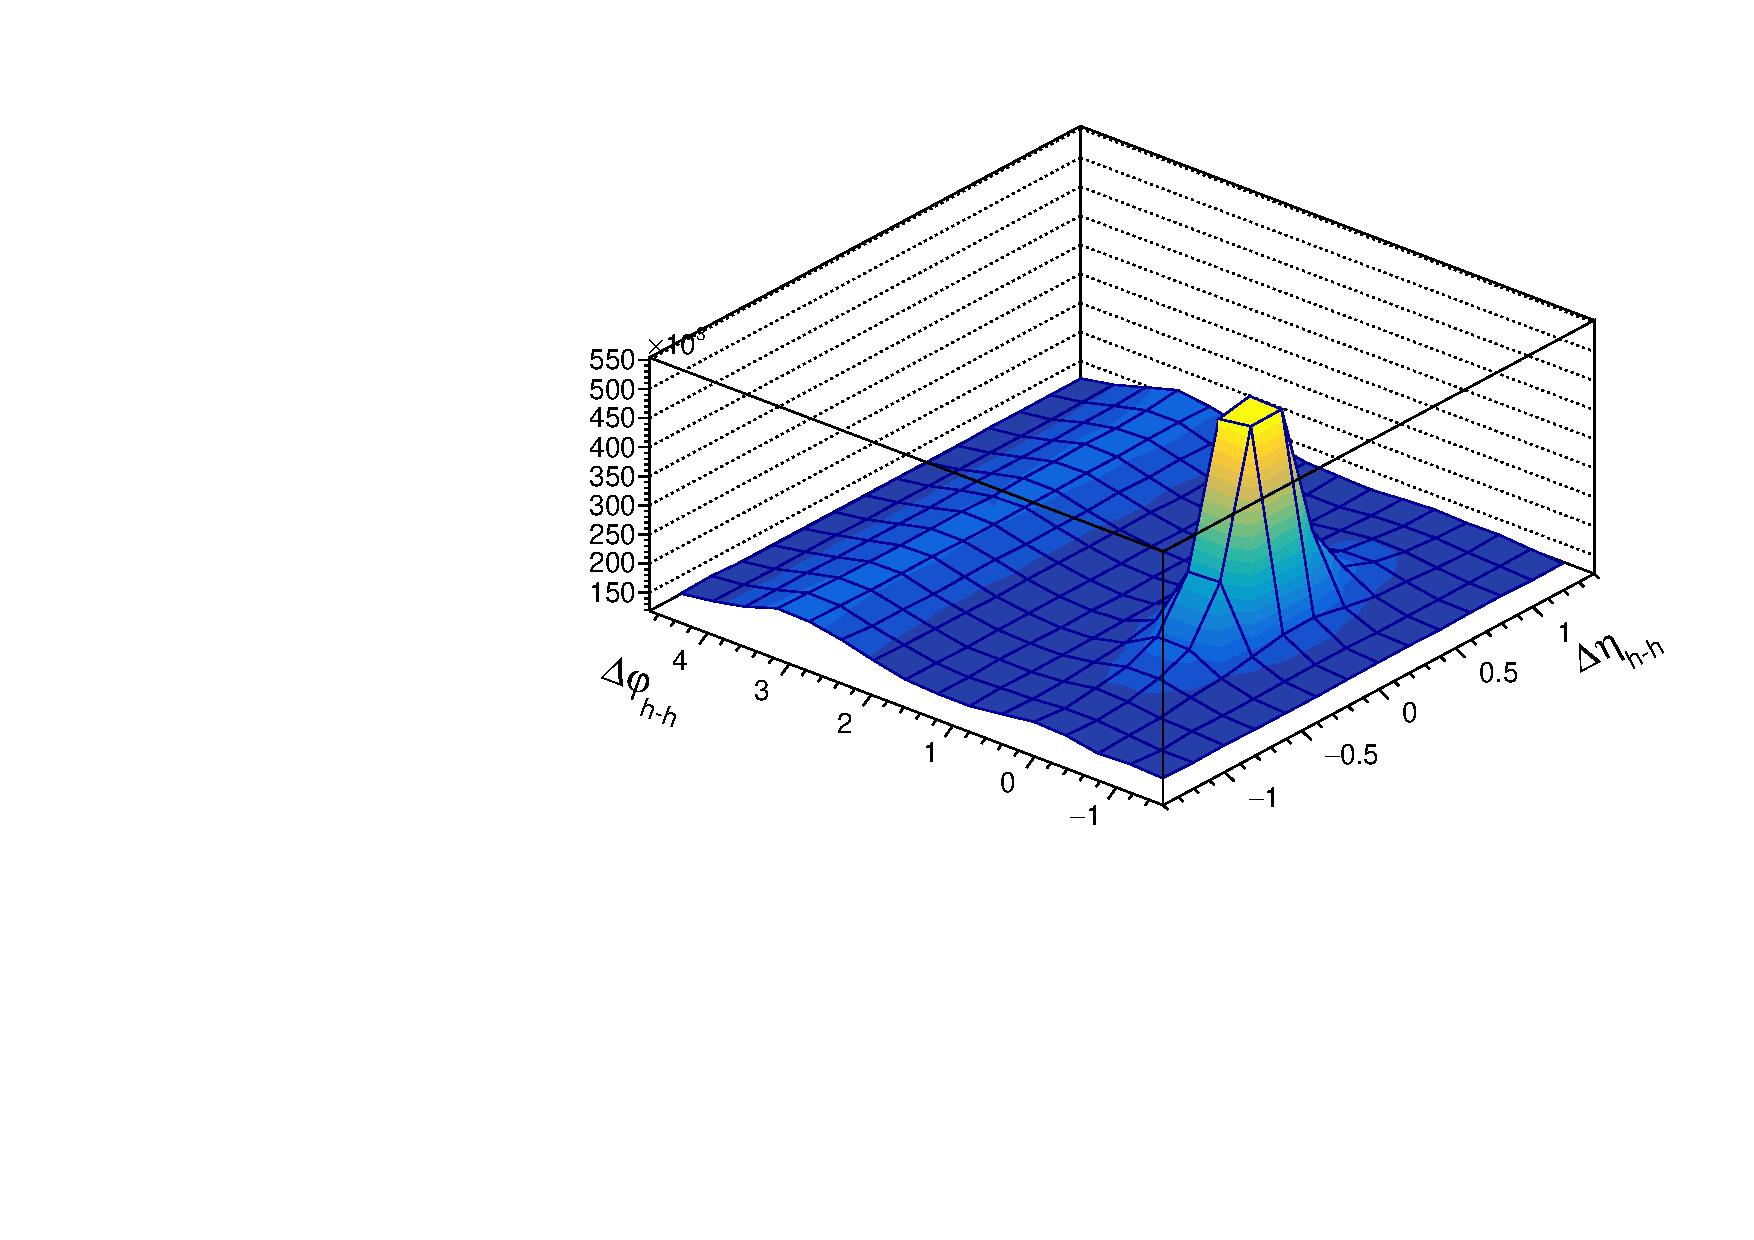
\includegraphics[width=3in]{figures/h_h_2d_mixcor_0_20.pdf}}
\end{subfigure}
\caption{Per-trigger 2-D h-$p\pi$ (left) and h-h (right) angular correlations for the 0-20\% multiplicity bin after acceptance corrections. Note that the triangular shape in $\Delta\eta$ is no longer present.}
\label{mixcor2d_0_20}
\end{figure}

\begin{figure}[ht]
\centering
\begin{subfigure}{
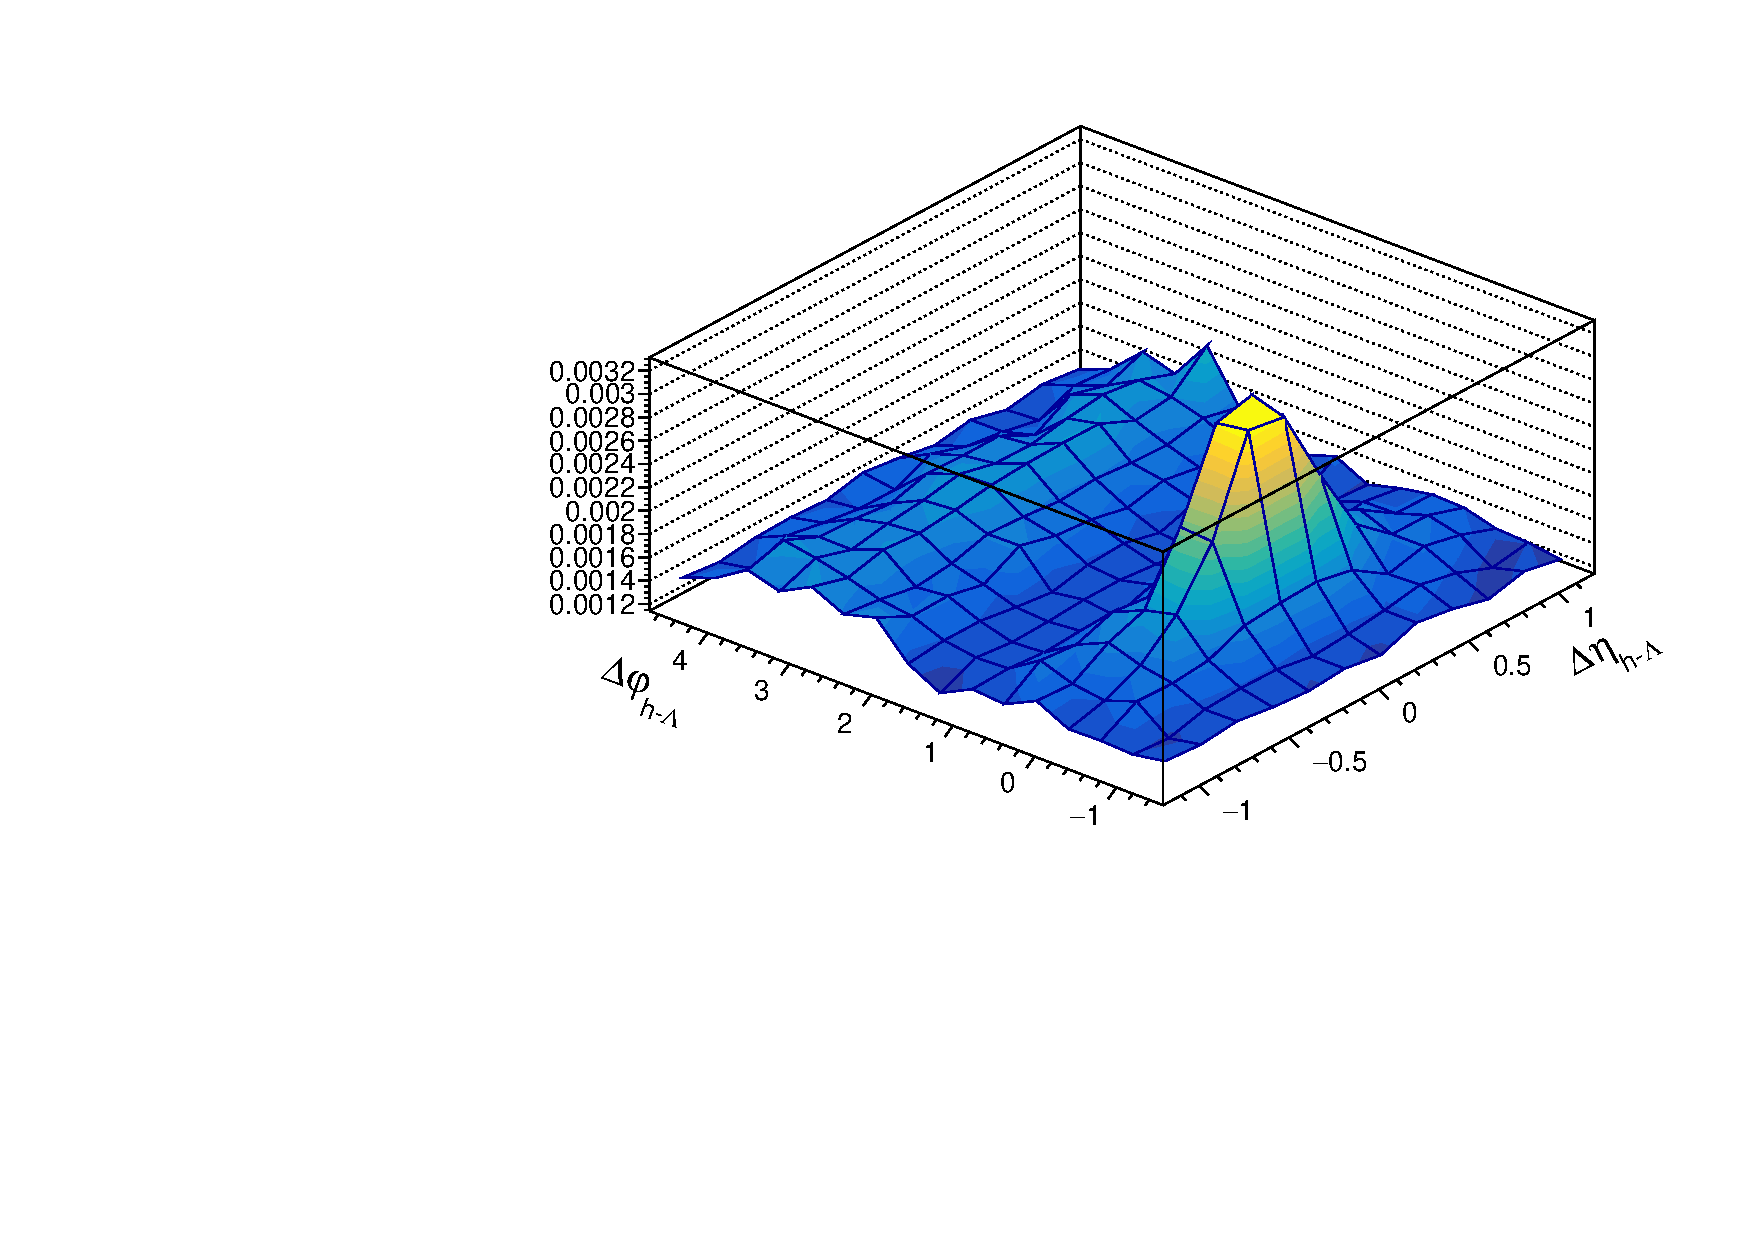
\includegraphics[width=3in]{figures/h_lambda_2d_mixcor_20_50.pdf}}
\end{subfigure}
\begin{subfigure}{
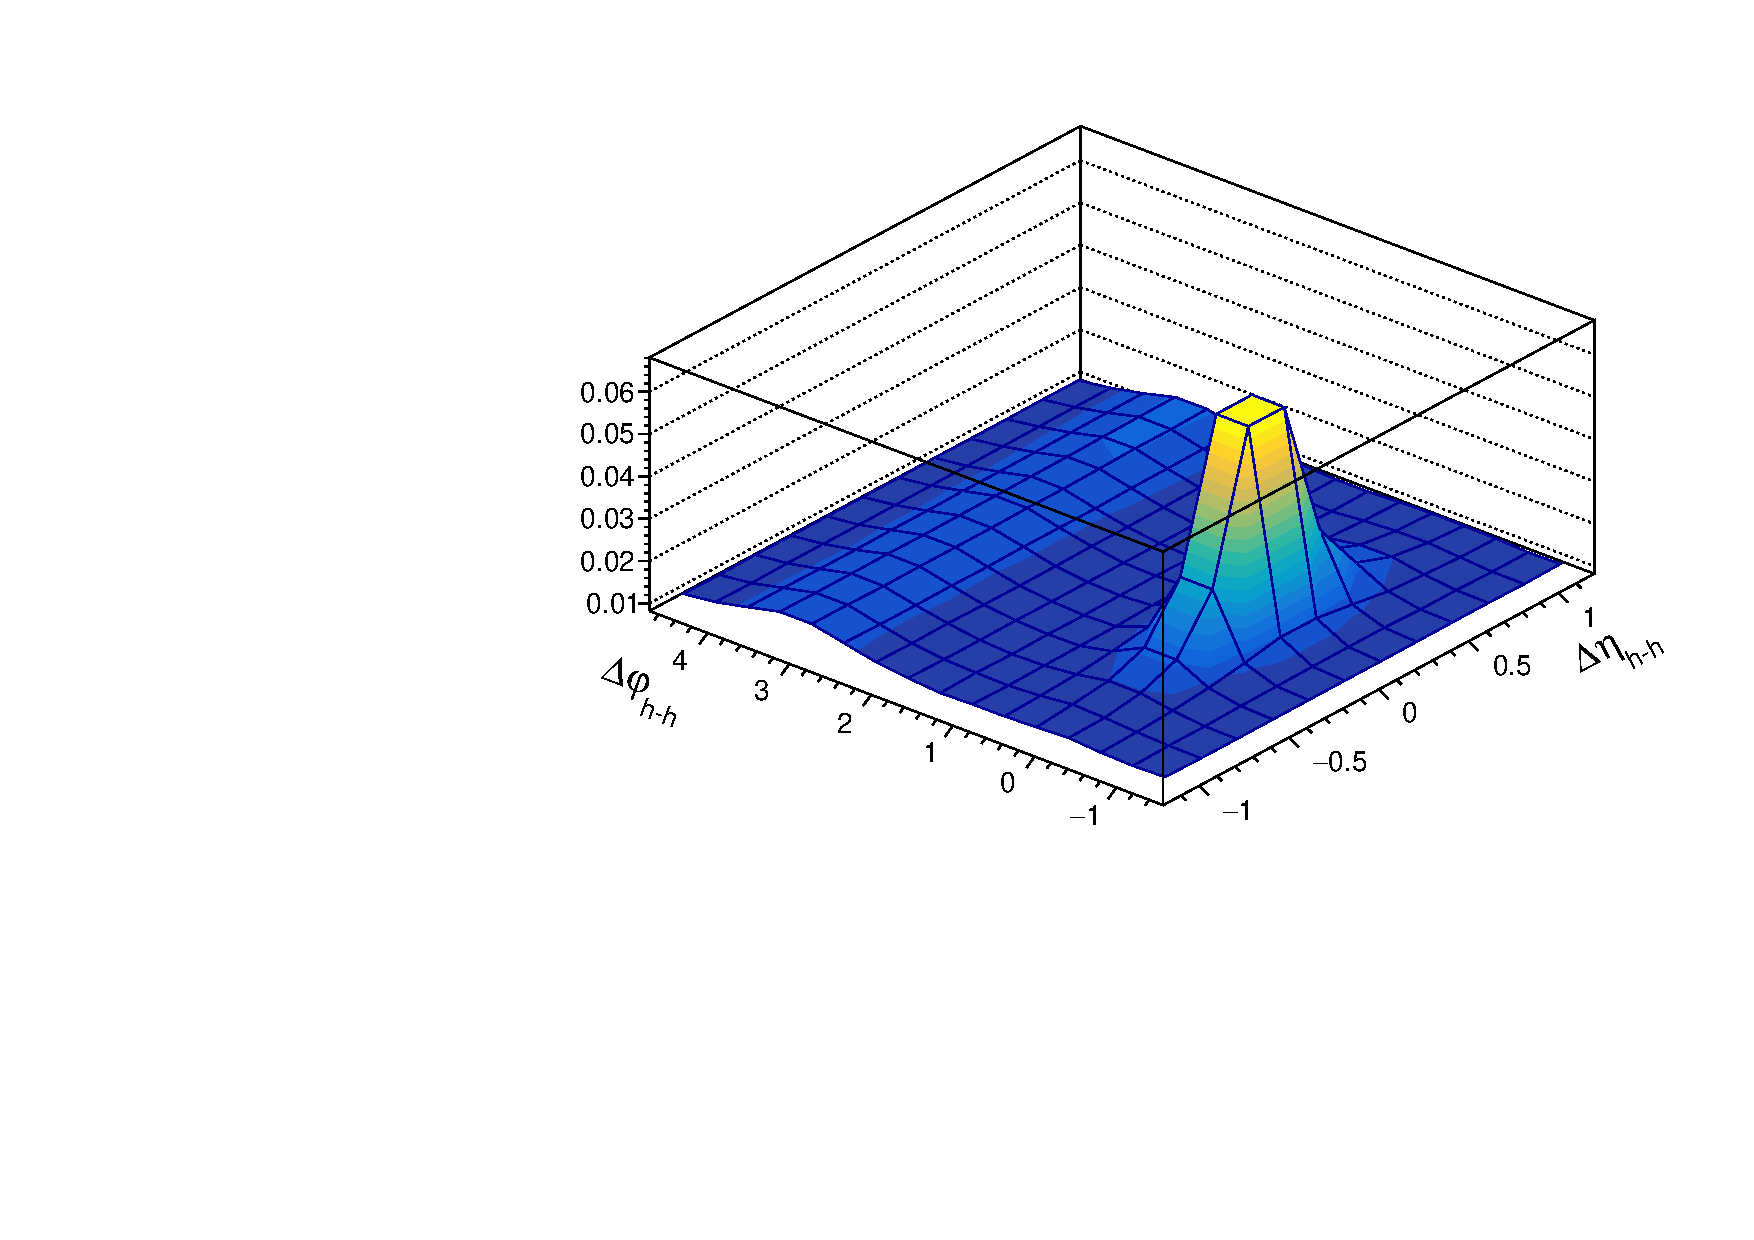
\includegraphics[width=3in]{figures/h_h_2d_mixcor_20_50.pdf}}
\end{subfigure}
\caption{Per-trigger 2-D h-$p\pi$ (left) and h-h (right) angular correlations for the 20-50\% multiplicity bin after acceptance corrections. Note that the triangular shape in $\Delta\eta$ is no longer present.}
\label{mixcor2d_20_50}
\end{figure}

\begin{figure}[ht]
\centering
\begin{subfigure}{
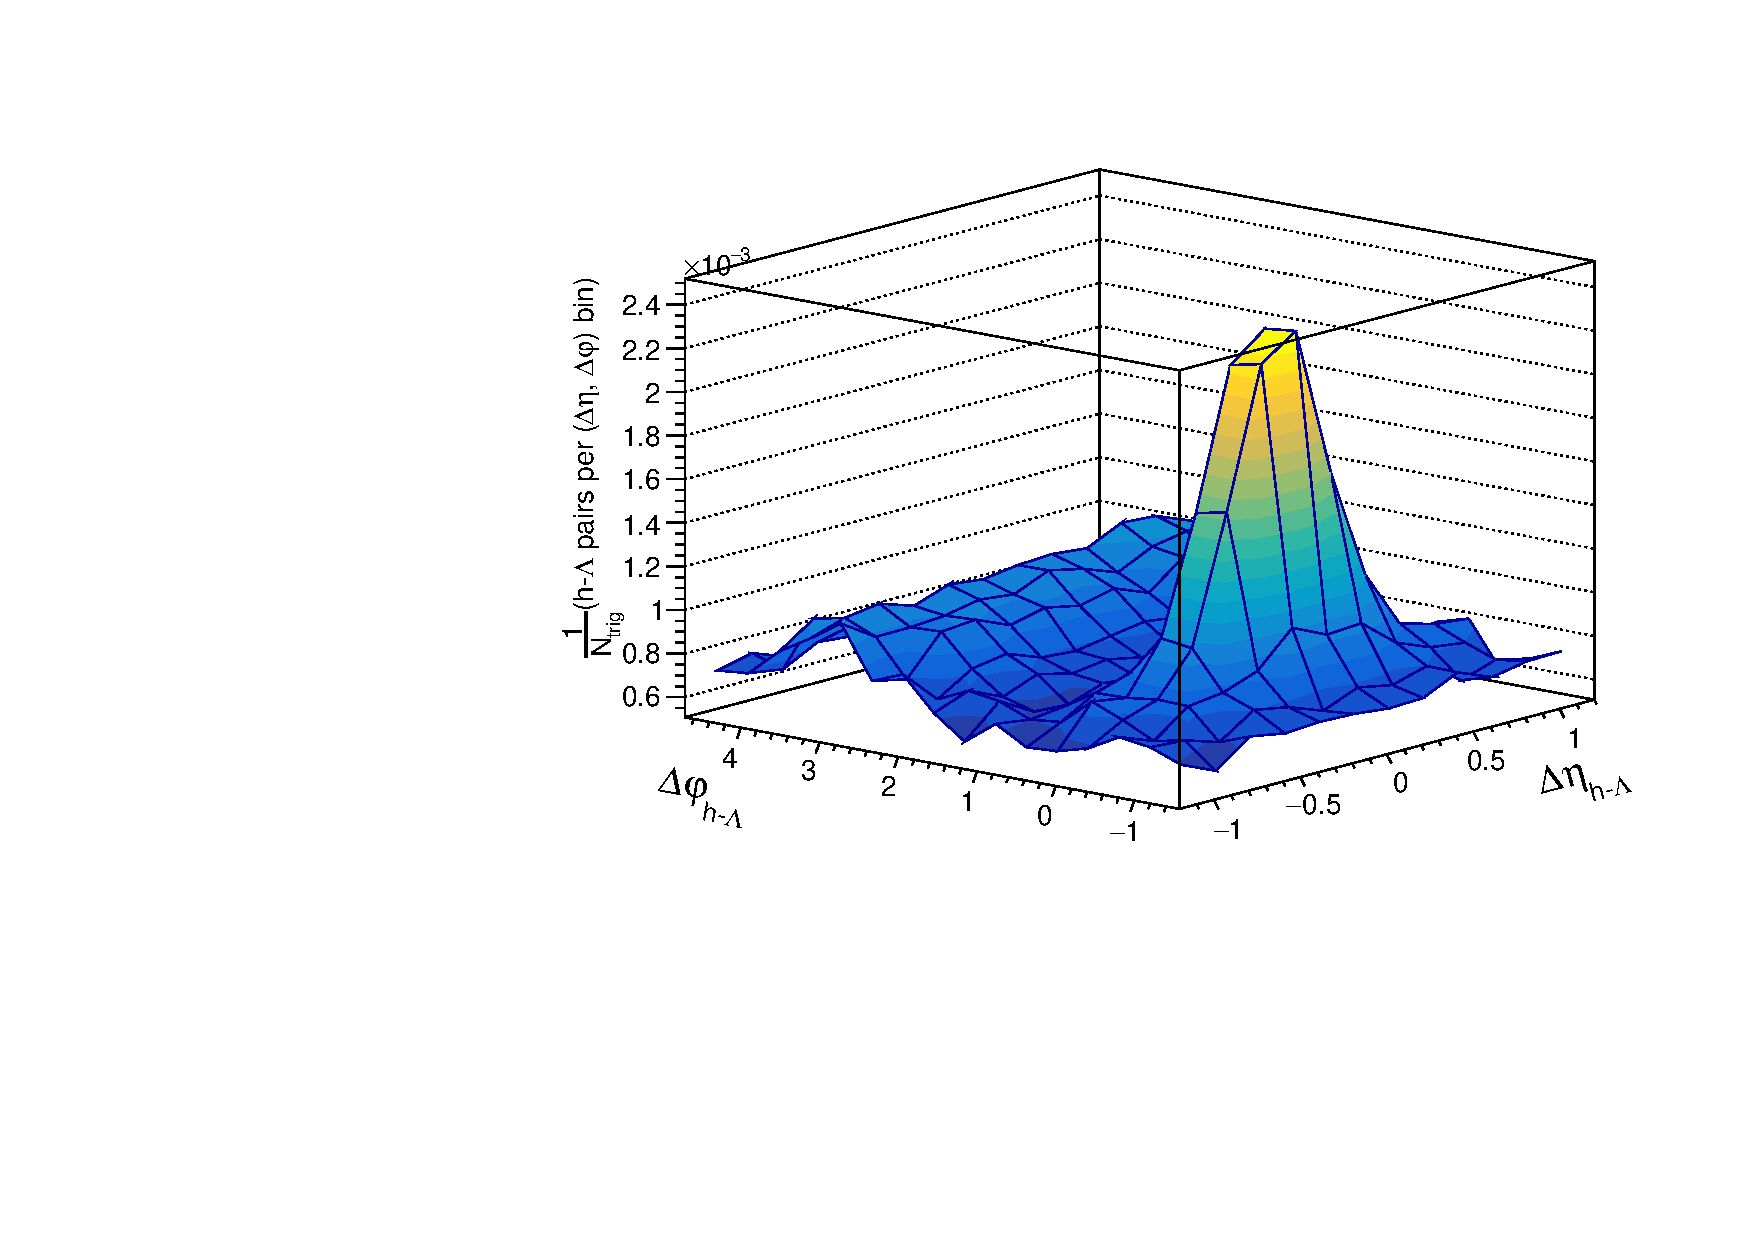
\includegraphics[width=3in]{figures/h_lambda_2d_mixcor_50_80.pdf}}
\end{subfigure}
\begin{subfigure}{
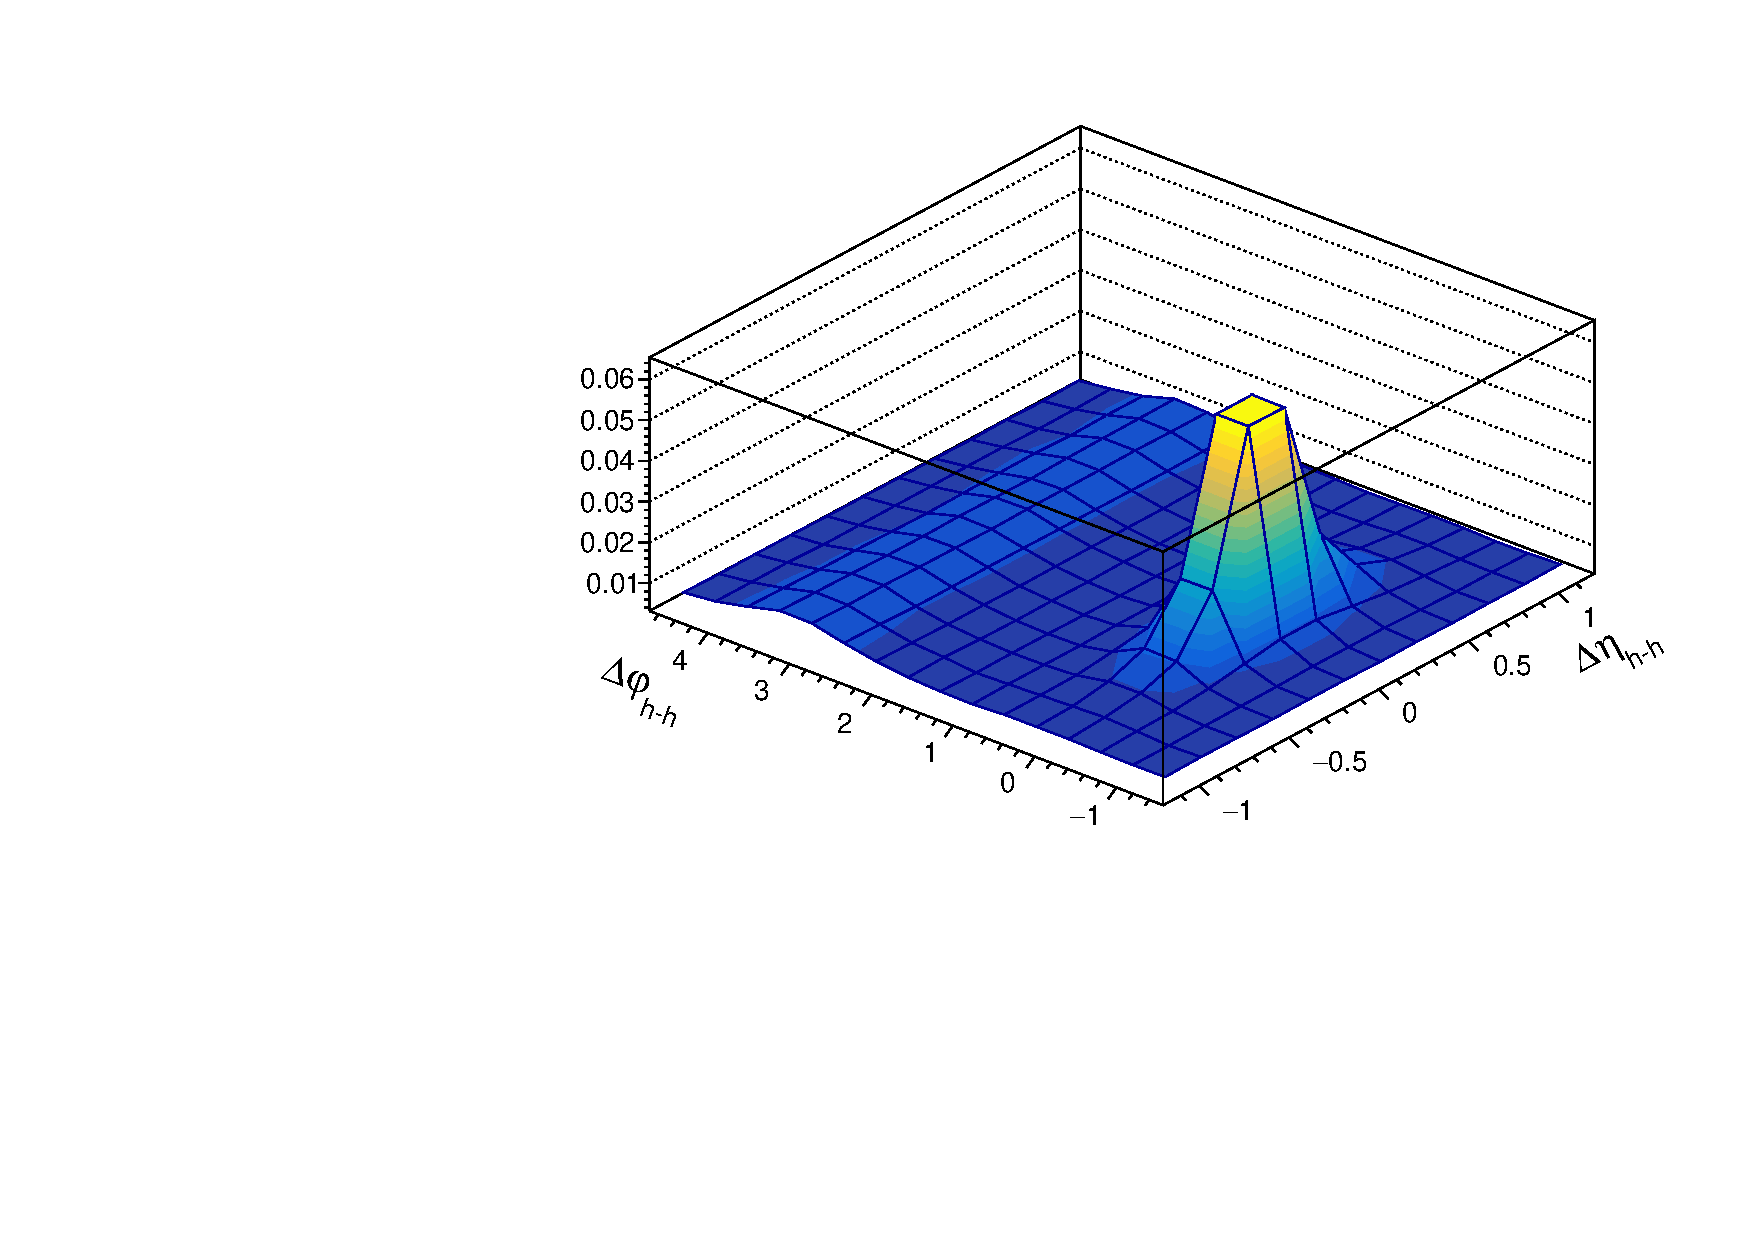
\includegraphics[width=3in]{figures/h_h_2d_mixcor_50_80.pdf}}
\end{subfigure}
\caption{Per-trigger 2-D h-$p\pi$ (left) and h-h (right) angular correlations for the 50-80\% multiplicity bin after acceptance corrections. Note that the triangular shape in $\Delta\eta$ is no longer present.}
\label{mixcor2d_50_80}
\end{figure}

\clearpage


\subsection{Reconstruction Efficiency}
\label{reconstruction_efficiency}
In this section we investigate the reconstruction efficiency of the $\Lambda$, trigger and associated hadrons.

\subsubsection{$\Lambda$ Reconstruction Efficiency}
\label{lambda_efficiency}

To estimate the $\Lambda$ reconstruction efficiency, we compare $\Lambda$ yields reconstructed using the V0 finder to the true $\Lambda$ yields using the MC production LHC17f2b\_FAST (anchored to LHC16q\_FAST production). The efficiency was calculated using the following formula:

\begin{align*}
	\varepsilon_{\Lambda} &=  \frac{N_{\Lambda\text{, reco with V0 finder}}}{N_{\Lambda\text{, real MC yield}}},
\end{align*}

where each $\Lambda$ in $N_{\Lambda\text{, reco with V0 finder}}$ meets the following criteria:

\begin{itemize}
	\item Found in the list of offline V0s
	\item $|\eta_{V0}| \leq 0.8$
	\item The daughter $p, \pi$ pass the daughter track cuts outlined in Section \ref{daughtercuts}
	\item The daughter $p, \pi$ tracks have corresponding real $p, \pi$ in the MC stack
	\item The corresponding MC stack $p, \pi$ daughters come from the same mother $\Lambda$ (also in MC stack)
\end{itemize}

and each $\Lambda$ in $N_{\Lambda\text{, real MC yield}}$ meets the following criteria:

\begin{itemize}
	\item Found in the MC stack
	\item $|\eta_{\Lambda}| \leq 0.8$
	\item The $\Lambda$ decays to $p\pi$
\end{itemize}
As we require the MC $\Lambda$ to decay to $p\pi$, we must correct for the branching ratio (63.9\%), which is discussed at the end of Section \ref{signal_scaling}.

While previous analyses focus solely on primary $\Lambda$s (exlcuding $\Omega$ and $\Xi$ contamination), there is no requirement for either the V0-reconstructed $\Lambda$ or the MC-generated $\Lambda$ to be a primary particle. As this analysis is mostly interested in the $\Lambda$ due to its strange quark content, whether or not the $\Lambda$ came from a cascade decay is irrelevant. This is important to note when making comparisons between this analysis and previous analyses, as secondary contamination from cascades accounts for nearly 20\% of all $\Lambda$s.

As mentioned in Section \ref{lambda_reconstruction}, both the $\Lambda$ and the $\bar{\Lambda}$ were combined together for this efficiency calculation (it was verified that their efficiencies are the same). Efficiencies were calculated as a function of $p_T$, $\eta$, $\varphi$, Event Z vertex, and Multiplicity. However, the final efficiency correction was applied as a function of $p_T$, $\eta$ and multiplicity and can be seen in Figures \ref{lambda_eff_pt} and \ref{lambda_eff_eta}. The multiplicity binning was chosen to be the same as the binning used for the final analysis (0-20\%, 20-50\%, 50-80\%).

\subsubsection{Trigger and Associated Hadron Reconstruction Efficiency}
\label{trigassoc_efficiency}

The trigger and associated hadron reconstruction efficiencies are calculated using the following formula:

\begin{align*}
	\varepsilon_{trig, assoc} &=  \frac{N_{trig, assoc\text{, reco yield}}}{N_{trig, assoc\text{, real MC yield}}},
\end{align*}

where each trigger or associated hadron in $N_{trig, assoc\text{, reco yield}}$ meets the following criteria:

\begin{itemize}
	\item Found in the list of AOD tracks
	\item $|\eta_{track}| \leq 0.8$
	\item The track passes the track cuts outlined in Section \ref{trigcuts} (trigger) or \ref{assoccuts} (associated)
	\item The track has a corresponding real track in the MC stack
	\item The corresponding MC track is either a pion, proton, kaon, electron or muon
\end{itemize}

and each trigger or associated hadron in $N_{trig, assoc\text{, real MC yield}}$ meets the following criteria:

\begin{itemize}
	\item Found in the MC stack
	\item $|\eta_{track}| \leq 0.8$
	\item The track is either a pion, proton, kaon, electron or muon
	\item The track is not a secondary particle (IsPhysicalPrimary() == true)
\end{itemize}

The efficiencies for both the trigger and associated hadrons as a function of $\it{p}_T$ are shown in Figure \ref{trigassoc_eff_plots}.

Even though only the $\Lambda$ efficiency shows a non-uniform dependence on $\eta$ and multiplicity, the final efficiency correction for all particles is applied as a function of $p_{T}$, $\eta$ and multiplicity.

As our correlation measurement depends on both the trigger and associated particle, we must combine the two efficiencies to get the overall efficiency for the pair.  This is done using the following formula:

\begin{align*}
    \epsilon_{pair} = \epsilon_{trig}*\epsilon_{assoc}
\end{align*}

This efficiency is corrected for on-the-fly as the pairs are being filled into the total correlation distribution by using a weighting factor equal to the inverse of $\epsilon_{pair}$. The same trigger efficiency used in the pair efficiency is then also to correct our $N_{trig}$ for our final per-trigger correlation in both the h-h and h-$\Lambda$ case.


\begin{figure}[ht]
\centering
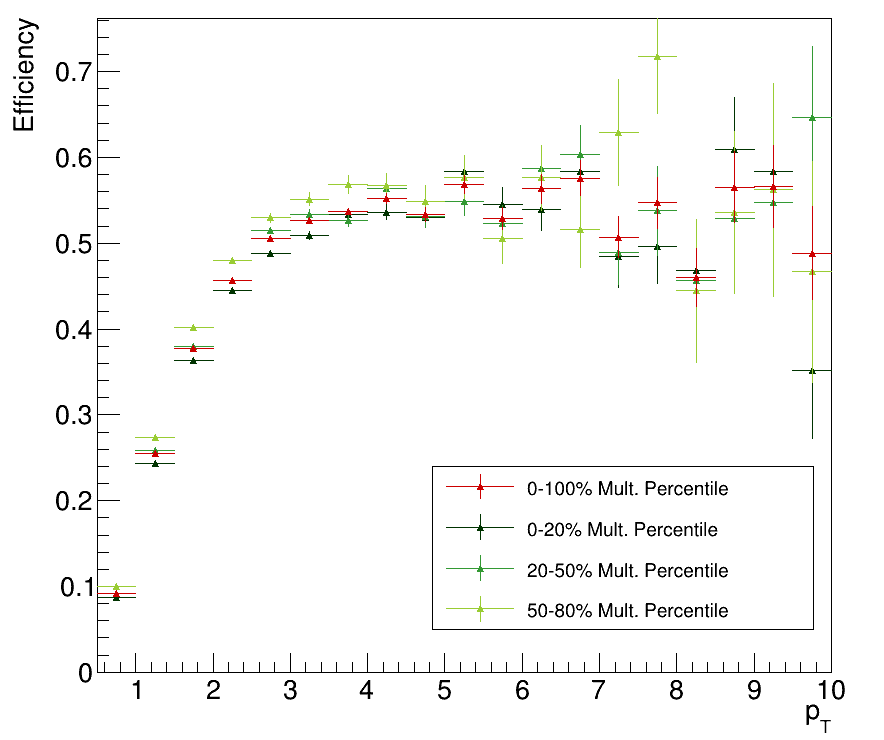
\includegraphics[width=4in]{figures/v0_efficiency_pt.png}
\caption{Efficiency vs. $p_T$ for $\Lambda$ reconstruction for each multiplicty bin, along with an integrated 0-100\% point in red. There appears to be a slight dependence on multiplicity, which is accounted for.}
\label{lambda_eff_pt}
\end{figure}

\begin{figure}[ht]
\centering
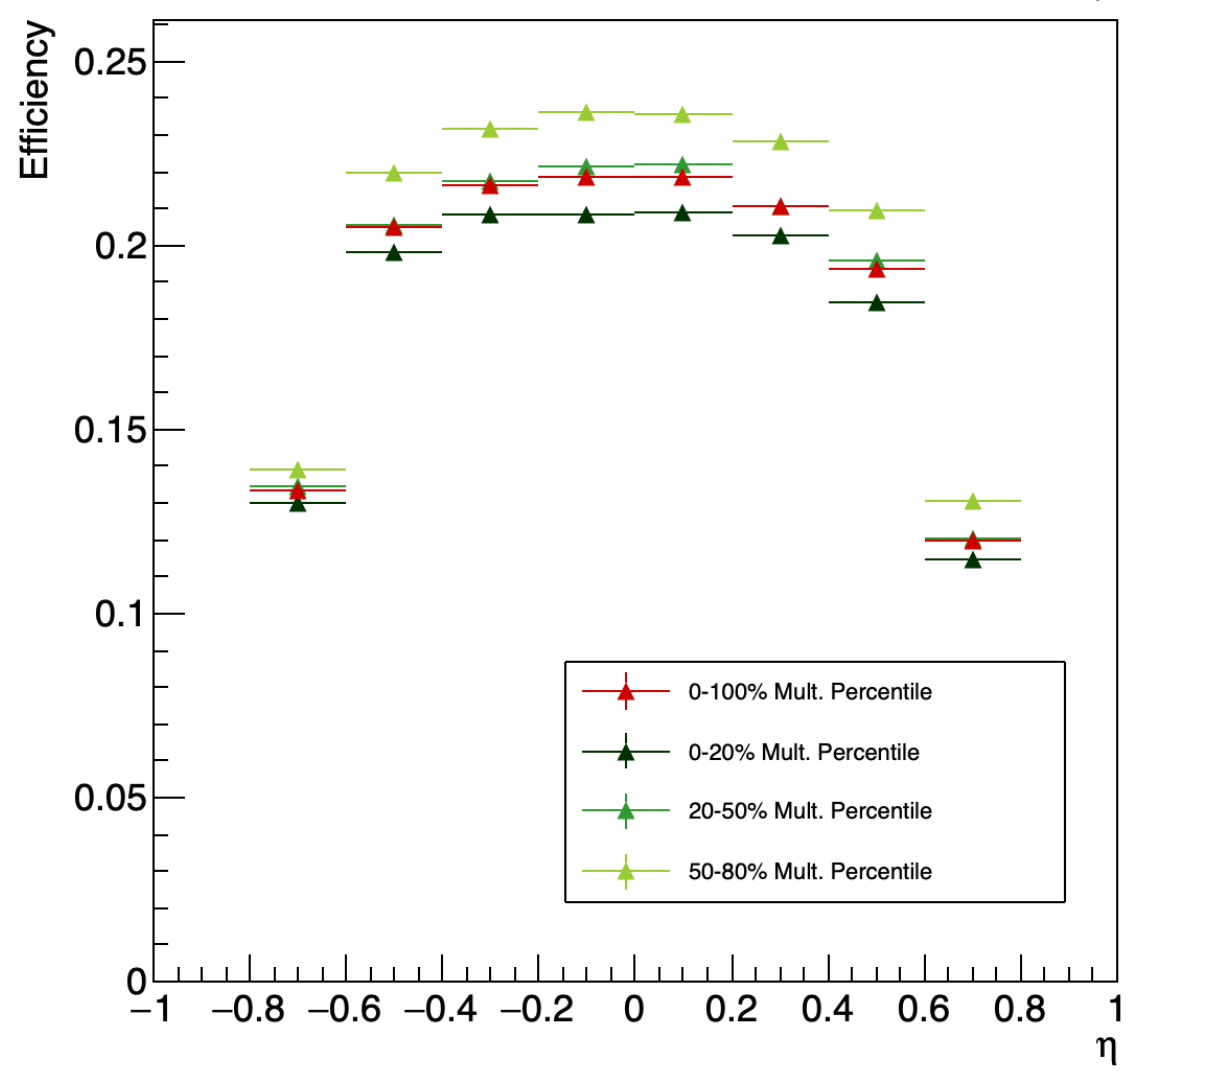
\includegraphics[width=4in]{figures/v0_efficiency_eta.png}
\caption{Efficiency vs. $\eta$ for $\Lambda$ reconstruction for each multiplicty bin, along with an integrated 0-100\% point in red. With wider bins (when compared to $p_{T}$), we clearly observe a multiplicity dependence, which is accounted for.}
\label{lambda_eff_eta}
\end{figure}


\begin{figure}[ht]
\centering
\begin{subfigure}{
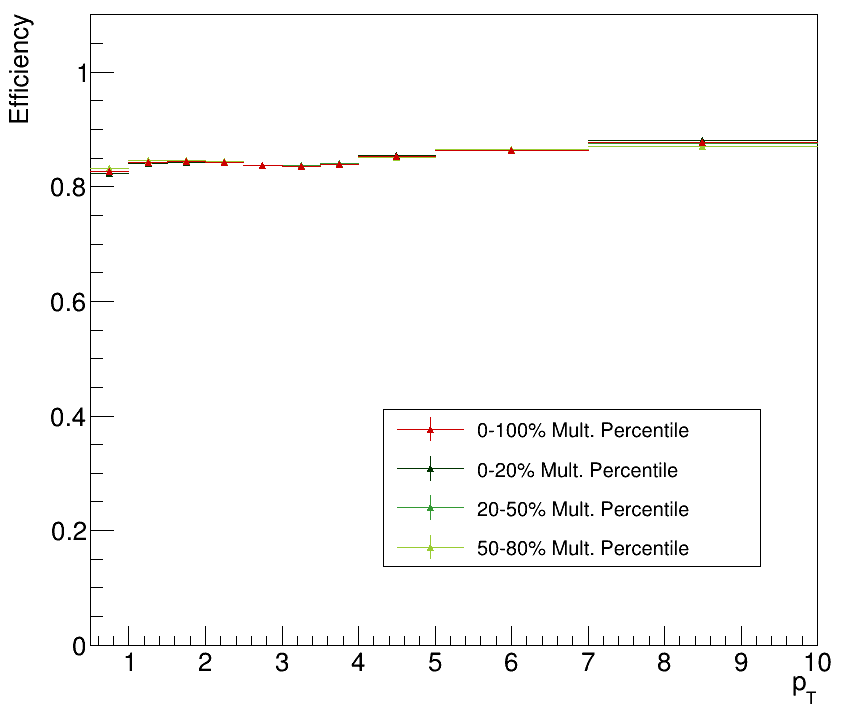
\includegraphics[width=3in]{figures/trigger_efficiency.png}}
\end{subfigure}
\begin{subfigure}{
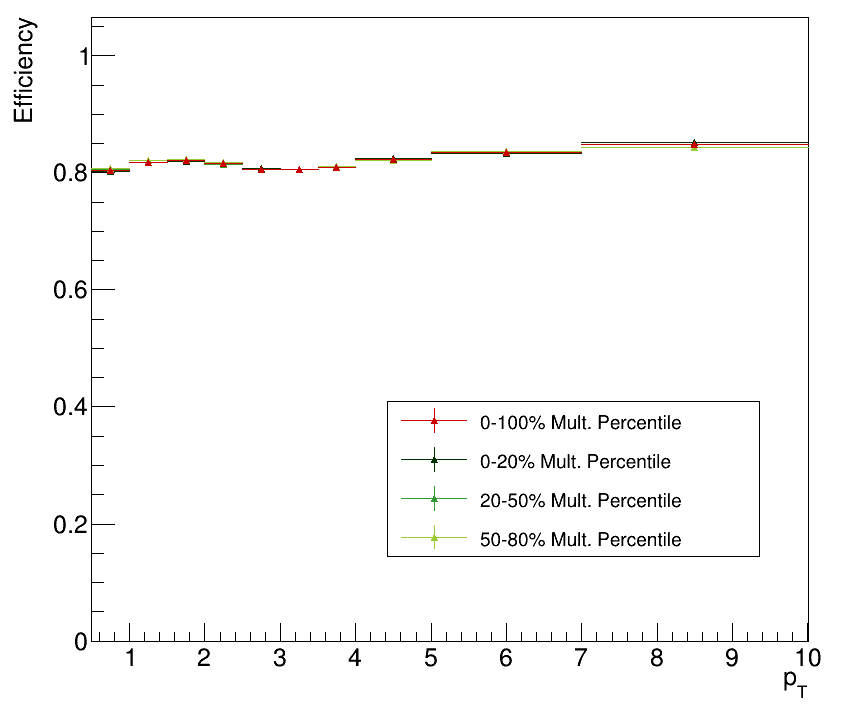
\includegraphics[width=3in]{figures/associated_efficiency.png}}
\end{subfigure}
\caption{Efficiency vs. $p_T$ for trigger (left) and associated (right) hadrons. Both are slightly above 80\% for the entire $p_\text{T}$ range.}
\label{trigassoc_eff_plots}
\end{figure}

\clearpage


\subsection{Track Merging Efficiency} 
\label{trackmerge_efficiency}

Many correlation studies are susceptible to track merging inefficiencies, whereby either the trigger or associated particle gets merged over by the other during the track reconstruction. This results in a dip at small angles in the $\Delta\eta\Delta\varphi$ distribution when compared to a similar distribution with no instances of track merging. As this effect cannot be seen directly in data due to the missing reconstructed tracks, it was investigated using our MonteCarlo sample, where we can compare the reconstructed tracks with the MC generated particles they were reconstructed from. While this effect is usually negligible and only relevant at extremely small angles ($\Delta\varphi < 0.01, \Delta\eta < 0.1$), in this analysis we see that this effect is more severe and occurs at larger angles ($\Delta\varphi < 1, \Delta\eta < 0.6$), shown in Figure \ref{trackmerge_diagram_lambda}. 

\begin{figure}[ht]
\centering
\begin{subfigure}{
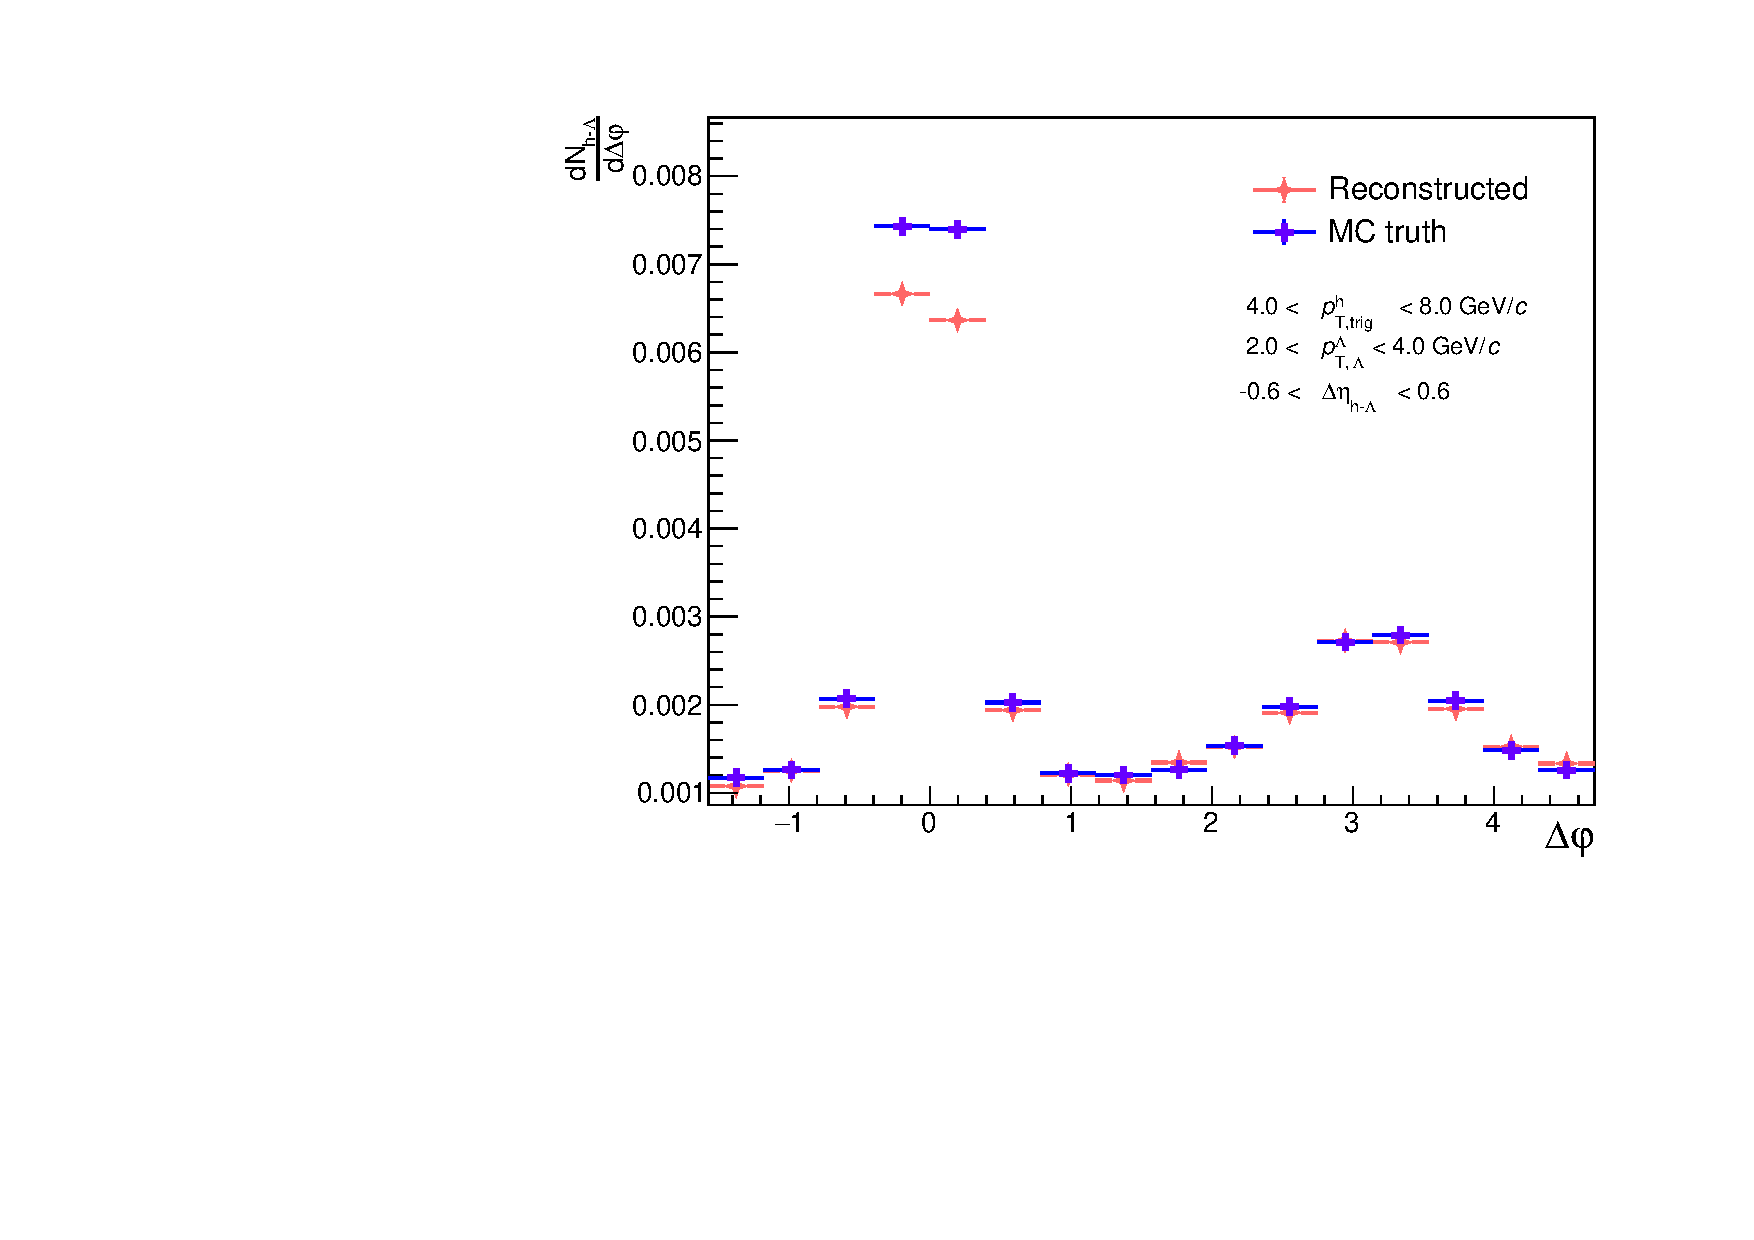
\includegraphics[width=3in]{figures/trackmerge_lambda_dphi_small_deta.pdf}}
\end{subfigure}
\begin{subfigure}{
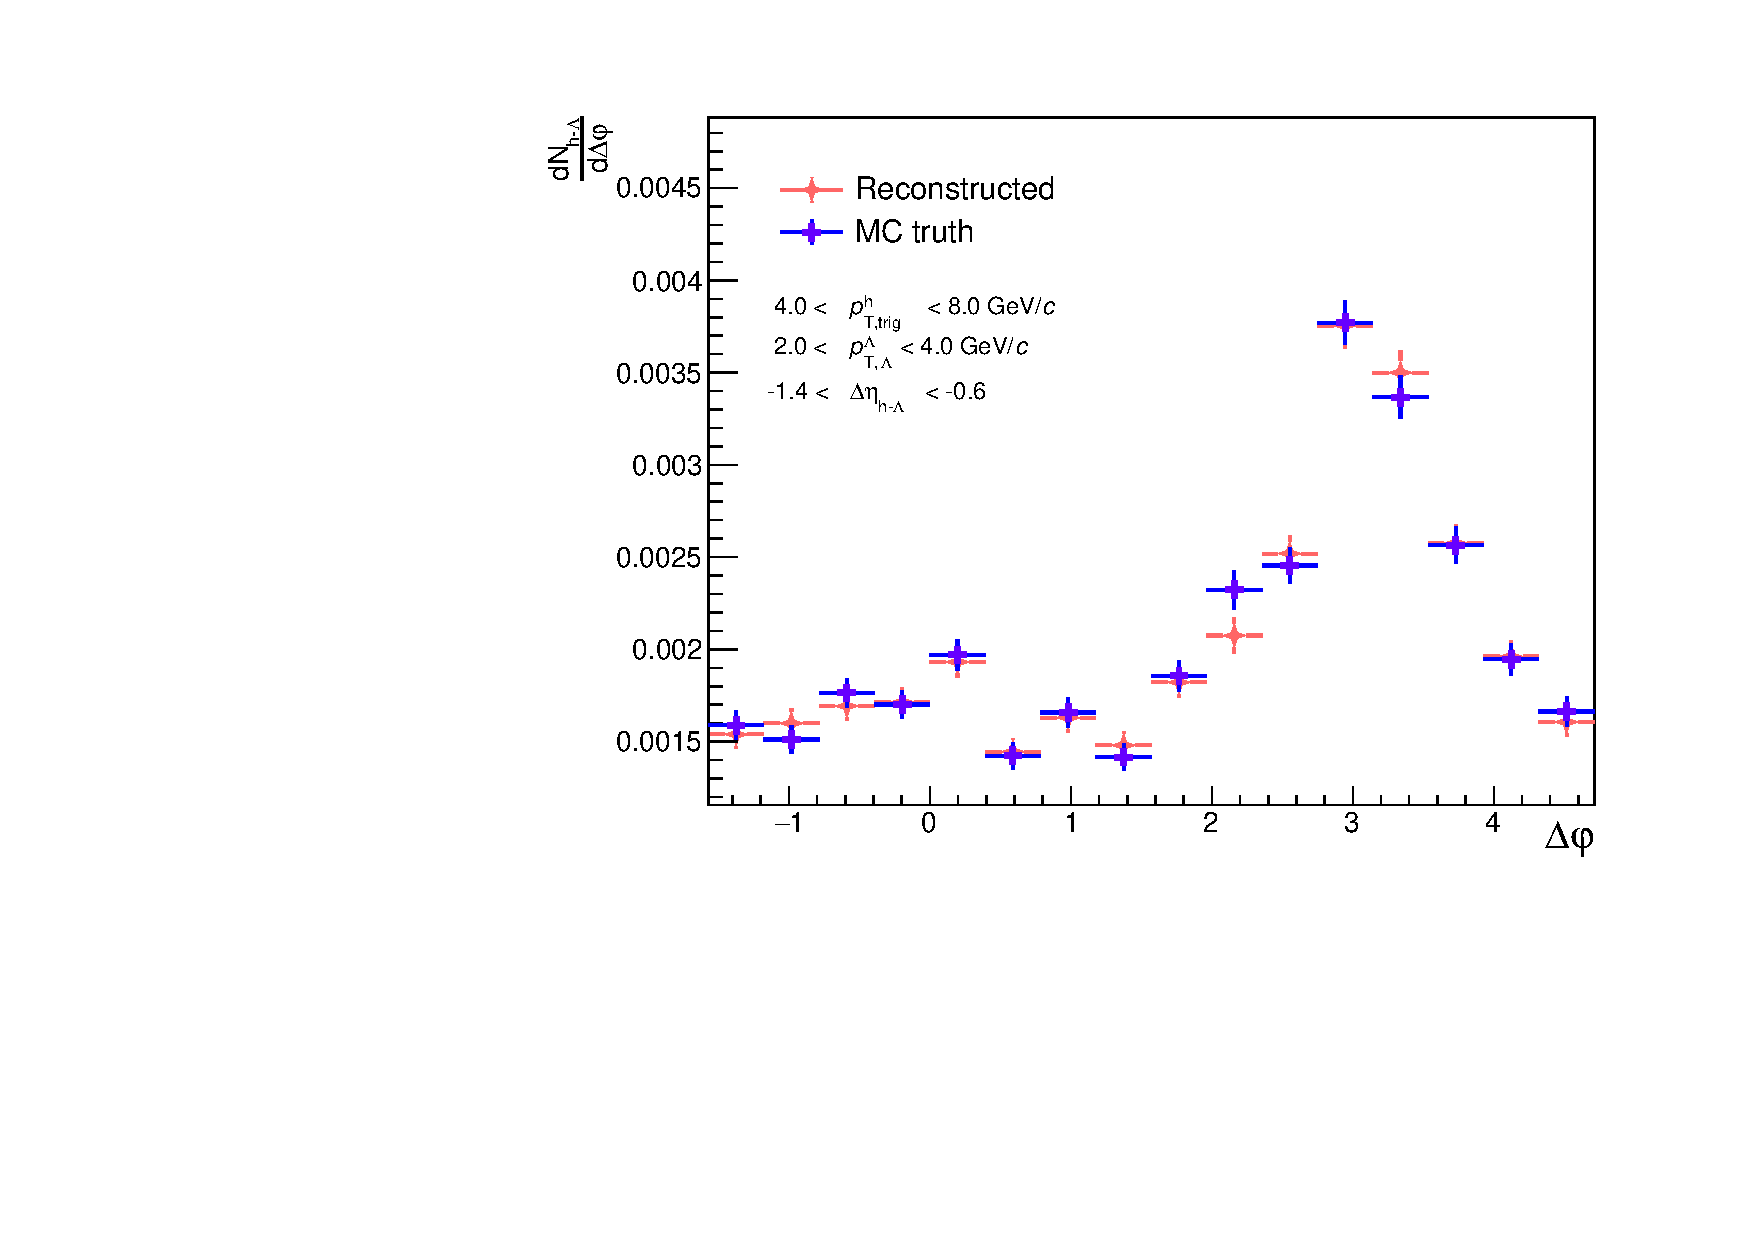
\includegraphics[width=3in]{figures/trackmerge_lambda_dphi_large_deta.pdf}}
\end{subfigure}
\caption{Demonstration of the track merging effect for $h-\Lambda$ pairs, whereby we see a dip in the reconstructed distribution at small $\Delta\varphi$ and $\Delta\eta$ when compared to the MC ground truth (left). This dip is not present at large $\Delta\eta$ (right), but we also lose nearly the entirety of our near-side peak.}
\label{trackmerge_diagram_lambda}
\end{figure}

The severity of this effect is likely due to two factors:
\begin{itemize}
\item The $\Lambda$ decay length is large ($c\tau \approx 10$ cm), meaning the daughter particles will have less hits in the detector than the trigger particle (which is produced at the primary vertex). As Kalman filtering (track reconstruction) favors the track with more hits, the $\Lambda$ daughter track is ``merged'' over by the trigger track.
\item The $\Lambda$ decay is asymmetric ($m_{p}/m_{\pi} \approx 7$), so the $\Lambda$ and daughter proton end up with similar momenta (and thus $\varphi$ and $\eta$). This means that whenever a proton from a $\Lambda$ decay is ``merged'' over by a trigger track, an $h-\Lambda$ pair with small $\Delta\varphi, \Delta\eta$ is lost.
\end{itemize}

To see how the decay length can affect the track merging, we can measure the $\Delta\eta\Delta\varphi$ distributions for $h-$pion pairs in our MonteCarlo sample where the pion is secondary--meaning it came from a weak decay with decay length $>$ 2cm--and compare it to the same ratio for $h-$pion pairs where the pion is primary. The result is shown in Figure \ref{trackmerge_hpion}. All reconstructed triggers and pions are selected from the AOD track list and pass our trigger and daughter cuts from Sections \ref{trigcuts} and \ref{daughtercuts}, respectively (with the caveat being that the pions are required to have a corresponding entry in the MC stack and that entry is either secondary or primary). All distributions were corrected for detector acceptance using the procedure described in Section \ref{mixed_event_correction}, and all distributions were corrected for efficiency (where we use the efficiency of primary particles in the primary case and secondary particles in the secondary case) We clearly observe a large suppression in the near side of the reconstructed distributions when compared to the ground truth for the h-secondary pion case, but no significant suppression for the h-primary pion case. As such, we conclude that this suppression is at least in part due to the decay length of the $\Lambda$, as all particles that come from $\Lambda$s are secondaries (by a long shot).

\begin{figure}[ht]
\centering
\begin{subfigure}{
\includegraphics[width=3in]{figures/h_pion_2d_secondary.png}}
\end{subfigure}
\begin{subfigure}{
\includegraphics[width=3in]{figures/h_pion_2d_primary.png}}
\end{subfigure}
\caption{The  reconstructed/ground truth 2d $\Delta\eta\Delta\varphi$ for h-(secondary pions) (left) and h-(primary pions) (right). The suppression at smaller $\Delta\eta, \Delta\varphi$ is clearly seen in the secondary case, but is not observable in the primary case.}
\label{trackmerge_hpion}
\end{figure}

We can also observe the $p_\text{T}$ dependence of this effect by looking at the reconstructed and ground truth $h-$(secondary pion) $\Delta\varphi$ distributions in a low ($1.0 < p_{T} < 2.0$) and high($2.0 < p_{T} < 4.0$) bin. The result is shown in Figure \ref{trackmerge_pt_dependence}. We clearly observe a suppression in the near side of the reconstructed distribution for the high $p_\text{T}$ bin, but not for the low $p_\text{T}$ bin.  This is consistent with the decay length dependence shown in the previous figures, as decay length is roughly proportional to $p_\text{T}$.

\begin{figure}[ht]
\centering
\begin{subfigure}{
\includegraphics[width=3in]{figures/h_pion_dphi_secondary_0_2.pdf}}
\end{subfigure}
\begin{subfigure}{
\includegraphics[width=3in]{figures/h_pion_dphi_secondary_2_4.pdf}}
\end{subfigure}
\caption{The  reconstructed and ground truth $\Delta\varphi$  distributions in the $-1.2 < \Delta\eta < 1.2$ region for h-(secondary pions) with $0.15 < p_{T, \pi} < 2$ (left) and $2 < p{T, \pi} < 4$ (right). The suppression at smaller $\Delta\eta, \Delta\varphi$ is clearly seen in the higher momentum bin, but not present in the lower one.}
\label{trackmerge_pt_dependence}
\end{figure}

The $p_{T}$ dependence of this inefficiency demonstrates why this effect is so severe in the $h-\Lambda$ case (when compared analyses involving another secondary weak decay, like $h-K^{0}$ from \url{https://alice-notes.web.cern.ch/node/902}). Due to the asymmetry of the $\Lambda$ decay ($m_{p}/m_{\pi} \approx 7$), the daughter proton receives most of the momentum. Therefore when we are investigating $h-\Lambda$ correlations within $2 < p_{T, \Lambda} < 4$ GeV/c, any inefficiencies present in the corresponding h-(daughter proton) distribution with the same associated momentum would also be present in our final $h-\Lambda$ distribution within the same $\Delta\varphi, \Delta\eta$ range. As we've demonstrated in Figure \ref{trackmerge_pt_dependence}, secondary charged particles with $2 < p_{T} < 4$ GeV/c see a large inefficiency, and therefore we would expect a similar inefficiency to be present in our $h-\Lambda$ distribution (which we've shown in Figure \ref{trackmerge_diagram_lambda}). Such an effect would not be as present in the $h-K^{0}$ case with the same associated momentum, both because the decay length is much shorter (2 cm vs 10 cm), and the $K^{0}$ decay is symmetric, meaning the daughter pions will have a momentum that is much lower than the mother (and therefore less affected by this inefficiency).


We have investigated all of the following techniques to correct for this effect:
\begin{itemize}
\item Applying a $\Delta\varphi^{*}$ correction, described \href{here}{https://alice-notes.web.cern.ch/node/902}: While $\Delta\varphi$ and $\Delta\varphi^{*}$ are different, they are correlated enough that in order to remove this effect we had to cut on $|\Delta\varphi^{*}| < 0.7$, which removes a significant amount of our near-side yield in the corresponding $\Delta\varphi$ distribution.
\item Applying a cut on the minimum distance between the fully reconstructed helices of the trigger and $\Lambda$ daughter proton (varied between 0.1 cm and 10 cm): Again, this cut removes roughly the same amount of near-side yield as the $\Delta\varphi^{*}$ cut, as this minimum distance is also highly correlated with $\Delta\varphi$.
\item Using the resonance technique for $\Lambda$ reconstruction (Section \ref{resonance_technique}): this drastically reduces the severity of this effect, but the statistical fluctuations introduced by the smaller S/B ratio make it difficult to investigate (see Section \ref{mc_closure} for more details)
\item Only correlating $h-\Lambda$ pairs where the charge of the $\Lambda$ daughter proton (or antiproton) is opposite to the trigger: This reduces the effect by a considerable amount, but reduces our overall correlation statistics by a factor of 2.
\item Selecting ``lower quality'' trigger tracks (instead of track bit kIsHybridGCG, we use similar cuts as our daughter particle): this reduces the effect, but introduces a large amount of secondary contamination. Furthermore, we would like this analysis to be compared with the $h-\phi$ analysis, and therefore want to maintain the same cuts on the trigger hadron.
\item Selecting ``higher quality''  $\Lambda$ daughter tracks (we use the kTrkGlobalNoDCA track filter bit): this completely eliminates this effect for $\Lambda$s reconstructed using the resonance technique (at the expense of a massive amount of signal), but for $\Lambda$s reconstructed using the V0 technique we are left with effectively no signal (an extremely small fraction of V0 daughter tracks have this filter bit set)
\end{itemize}

The most promising correction procedure is the one described in the AN here: \url{https://alice-notes.web.cern.ch/node/732}, which corrects for this inefficiency using a $\Delta\eta\Delta\varphi$ template generated from MonteCarlo. The formula for this correction is:
\begin{align*}
	C_{corr.}(\Delta\varphi, \Delta\eta) = C_{uncorr.}(\Delta\varphi, \Delta\eta)(\frac{C_{reco. MC}(\Delta\varphi, \Delta\eta)}{C_{real. MC}(\Delta\varphi, \Delta\eta)})^{-1}
\end{align*}

where $C_{corr.}$ is the corrected correlation, $C_{uncorr.}$ is the uncorrected correlation, and $\frac{C_{reco. MC}(\Delta\varphi, \Delta\eta)}{C_{real. MC}(\Delta\varphi, \Delta\eta)}$ is the angular efficiency template generated from MonteCarlo. This template is generated using a similar procedure as our MonteCarlo closure tests (see Section \ref{mc_closure}) by taking the fully acceptance and efficiency-corrected reconstructed $\Delta\eta\Delta\varphi$ distribution and dividing it by the ground-truth $\Delta\eta\Delta\varphi$ distribution, and is shown in Figure \ref{twotrack_templates}. The main difference between this template and the closure tests is that while the $\Lambda$s in the numerator were ``reconstructed'' using the V0 finder, they were verified to be true $\Lambda$s in MonteCarlo and the kinematics were taken from the corresponding MonteCarlo particle. This bypasses things like sideband subtraction and signal scaling, which are both performed in the standard MC closure tests. 

The templates are shown for each $p_{T}$ bin in Figure \ref{twotrack_templates}. These templates are applied in our final results (after the efficiency and acceptance corrections and sideband subtraction). The templates have been thoroughly verified to be independent of event multiplicity and MC event generator.

\clearpage

\begin{figure}[ht]
\centering
\begin{subfigure}{
\includegraphics[width=4in]{figures/twotrack_template.pdf}}
\end{subfigure}
\begin{subfigure}{
\includegraphics[width=4in]{figures/twotrack_template_lowpt.pdf}}
\end{subfigure}
\begin{subfigure}{
\includegraphics[width=4in]{figures/twotrack_template_highpt.pdf}}
\end{subfigure}
\caption{Templates for track merging correction in our central (2.0-4.0 GeV/c, top), lower (1.5-2.5 GeV/c, middle) and higher (2.5-4.0 GeV/c, bottom) $p_{T}$ bins. The templates were generated using the procedure described in this section, and are applied to the fully acceptance and efficiency-corrected correlation distributions after sideband-subtraction is performed. While it may be difficult to observe, the lower $p_{T}$ bin has a minimum dip of around 0.84, whereas the higher $p_{T}$ bin has a minimum dip of around 0.81, reflecting the $p_{T}$ dependence discussed in this section.}
\label{twotrack_templates}
\end{figure}

\clearpage

\section{Correlation Measurement Technique}
\label{corrsec}

\subsection{Full Correlation Measurement Method}

The per-trigger correlation is approximated for each multiplicity bin using the formula:

\begin{align}
\label{corrEq}
C_{trig}(\Delta\varphi, \Delta\eta) = \frac{1}{N_{trig}}\frac{B(0,0)*S(\Delta\varphi,\Delta\eta)}{B(\Delta\varphi, \Delta\eta)}
\end{align}

where $N_{trig}$ is the total number of hadrons in the $4 < p_{T} < 8$ GeV/c range that pass our trigger cuts described in Section \ref{trigcuts}, $S(\Delta\varphi, \Delta\eta)$ is the efficiency-corrected (Section \ref{trigassoc_efficiency}) same event correlation and $B(\Delta\varphi, \Delta\eta)$ is the efficiency-corrected mixed-event correlation.  To properly account for the acceptance effects, the mixed-event distribution is scaled to the value of the $(\Delta\varphi = 0, \Delta\eta = 0)$ bin of the same event distribution.

However, what is actually measured is an angular correlation of $h-(p\pi)$ pairs that is comprised of the real $h-\Lambda$ signal as well as a background of $h-(p\pi)$ pairs. The full correlation equation is then:

\begin{align}
\label{corrEq_withBG}
\begin{split}
    C_{h-\Lambda}(\Delta\varphi, \Delta\eta) = r_{\text{signal}}\biggl(&C_{(h-p\pi)^{US}_{\text{signal}}}(\Delta\varphi, \Delta\eta)\\
    &- r_{comb}*C_{(h-p\pi)^{US}_{\text{RSB,normalized}}}(\Delta\varphi, \Delta\eta)\biggr)
\end{split}
\end{align}

Where each term is defined as follows:
\begin{itemize}
	\item $C_{h-\Lambda}(\Delta\varphi, \Delta\eta)$: The final $h-\Lambda$ correlation distribution
	\item $C_{(h-p\pi)^{US}_{\text{signal}}}$: The $h-(p\pi)$ correlation in our signal region
	\item $C_{(h-p\pi)^{US}_{\text{RSB,normalized}}}(\Delta\varphi, \Delta\eta)$: The $h-(p\pi)$ correlation in the right sideband region (RSB) normalized to unity
	\item $r_{\text{signal}}$: Scaling factor used to account for fraction of the $h-\Lambda$ signal that is missed by choosing a finite signal region and for the branching ratio
	\item $r_{\text{comb}}$: Scaling factor used to account for combinatorial background in the $h-(p\pi)$ correlation
\end{itemize}

The calculations of $r_{\text{comb}}$ and $r_{\text{signal}}$ are described in the following sections.

\subsubsection{Combinatorial Background Removal}
\label{removecomb_v0}
Since we do not know which $p-\pi$ pairs came from a real $\Lambda$ decay, we must remove the contribution to the angular correlation structure due to the combinatorial background of $p-\pi$ pairs that did not come from a $\Lambda$.

To do this, h-($p\pi$) angular correlations are measured for unlike-sign $p\pi$ pairs within the right sideband (RSB) for each multiplicity bin. The correlation structure in the RSB is then normalized to its integral to give an estimate of the combinatorial background shape, as the RSB should contain little-to-no $p\pi$ pairs that came from a $\Lambda$. 

Next, the $h-p\pi$ angular correlation in our chosen sideband region is scaled to match the integral of our background in our signal region. However, this scaling is not performed directly as while the Signal/Background and Signal/(Signal + Background) ratios are the same for the single-particle $\Lambda$ distribution in a triggered event and its corresponding invariant mass axis in our $h-\Lambda$ distribution, the total yields are different. We therefore scale the $h-p\pi$ distribution in the RSB to the BG integral in our signal region found using the following formula:

\begin{align}
	h-p\pi \text{\space Combinatorial BG} := r_{Comb} = (\text{Integral of \space} h-p\pi \text{\space in Signal Region}) \times (1 - \frac{S}{S+B}),
\end{align}

where $S$ and $B$ are calculated bin-wise using the straight line backgrounds shown in Figures \ref{v0_mass} through \ref{v0_mass_highpt}.

Once the $h-p\pi$ angular correlation in the RSB is scaled to match the $h-p\pi$ Combinatorial BG, it is subtracted from the total $h-p\pi$ distribution in our signal region. 

\subsubsection{Signal Region Scaling}
\label{signal_scaling}
As our invariant mass signal region is finite, we must correct for the fraction of the $h-\Lambda$ signal that is missed in the tails of our invariant mass distribution. This is done using the following formula:

\begin{align}
	r_{\text{signal}} = (\text{Integral of residual in signal region} / \text{Integral of residual between 1.098 and 1.134})^{-1}
\end{align}

where ``1.098'' and ``1.134'' are the points in which we observe effectively zero signal in MonteCarlo (when reconstructed using the same technique with MC-verified $\Lambda$s). 

Once the scale factor is applied, we apply the branching ratio correction (1/0.639), and we are then left with the full $h-\Lambda$ 2D angular correlations and corresponding 1D $\Delta\varphi$ projection.

\subsection{Full h-$\Lambda$ and h-h Correlation Measurement}

Using Equation \ref{corrEq_withBG} and the efficiencies calculated in Section \ref{efficiency_acceptance}, we can plot the final 2D angular correlations for both h-$\Lambda$ and $h-h$ pairs, shown in for each $p_{T, associated}$ bin Figures \ref{h_lambda_2d} through \ref{h_h_2d_highpt}.


\begin{figure}[ht]
\centering
\begin{subfigure}{
\includegraphics[width=4in]{figures/h_lambda_2d_mixcor_0_20.pdf}}
\end{subfigure}
\begin{subfigure}{
\includegraphics[width=4in]{figures/h_lambda_2d_mixcor_20_50.pdf}}
\end{subfigure}
\begin{subfigure}{
\includegraphics[width=4in]{figures/h_lambda_2d_mixcor_50_80.pdf}}
\end{subfigure}
\caption{Per-trigger normalized 2D angular correlations for h-$\Lambda$ pairs in the 0-20\% (top), 20-50\% (center) and 50-80\% (bottom) multiplicity bins in our central (2.0 - 4.0 GeV/c) $p_{T, assoc}$ bin.}
\label{h_lambda_2d}
\end{figure}

\clearpage
\begin{figure}[ht]
\centering
\begin{subfigure}{
\includegraphics[width=4in]{figures/h_lambda_2d_mixcor_0_20_lowpt.pdf}}
\end{subfigure}
\begin{subfigure}{
\includegraphics[width=4in]{figures/h_lambda_2d_mixcor_20_50_lowpt.pdf}}
\end{subfigure}
\begin{subfigure}{
\includegraphics[width=4in]{figures/h_lambda_2d_mixcor_50_80_lowpt.pdf}}
\end{subfigure}
\caption{Per-trigger normalized 2D angular correlations for h-$\Lambda$ pairs in the 0-20\% (top), 20-50\% (center) and 50-80\% (bottom) multiplicity bins in our lower (1.5 - 2.5 GeV/c) $p_{T, assoc}$ bin.}
\label{h_lambda_2d_lowpt}
\end{figure}

\clearpage

\begin{figure}[ht]
\centering
\begin{subfigure}{
\includegraphics[width=4in]{figures/h_lambda_2d_mixcor_0_20_highpt.pdf}}
\end{subfigure}
\begin{subfigure}{
\includegraphics[width=4in]{figures/h_lambda_2d_mixcor_20_50_highpt.pdf}}
\end{subfigure}
\begin{subfigure}{
\includegraphics[width=4in]{figures/h_lambda_2d_mixcor_50_80_highpt.pdf}}
\end{subfigure}
\caption{Per-trigger normalized 2D angular correlations for h-$\Lambda$ pairs in the 0-20\% (top), 20-50\% (center) and 50-80\% (bottom) multiplicity bins in our higher (2.5 - 4.0 GeV/c) $p_{T, assoc}$ bin.}
\label{h_lambda_2d_highpt}
\end{figure}

\clearpage
\begin{figure}[ht]
\centering
\begin{subfigure}{
\includegraphics[width=4in]{figures/h_h_2d_mixcor_0_20.pdf}}
\end{subfigure}
\begin{subfigure}{
\includegraphics[width=4in]{figures/h_h_2d_mixcor_20_50.pdf}}
\end{subfigure}
\begin{subfigure}{
\includegraphics[width=4in]{figures/h_h_2d_mixcor_50_80.pdf}}
\end{subfigure}
\caption{Per-trigger normalized 2D angular correlations for h-h pairs in the 0-20\% (top), 20-50\% (center) and 50-80\% (bottom) multiplicity bins in our central (2.0 - 4.0 GeV/c) $p_{T}$ bin.}
\label{h_h_2d}
\end{figure}

\clearpage
\begin{figure}[ht]
\centering
\begin{subfigure}{
\includegraphics[width=4in]{figures/h_h_2d_mixcor_0_20_lowpt.pdf}}
\end{subfigure}
\begin{subfigure}{
\includegraphics[width=4in]{figures/h_h_2d_mixcor_20_50_lowpt.pdf}}
\end{subfigure}
\begin{subfigure}{
\includegraphics[width=4in]{figures/h_h_2d_mixcor_50_80_lowpt.pdf}}
\end{subfigure}
\caption{Per-trigger normalized 2D angular correlations for h-h pairs in the 0-20\% (top), 20-50\% (center) and 50-80\% (bottom) multiplicity bins in our lower (1.5 - 2.5 GeV/c) $p_{T}$ bin.}
\label{h_h_2d_lowpt}
\end{figure}

\clearpage
\begin{figure}[ht]
\centering
\begin{subfigure}{
\includegraphics[width=4in]{figures/h_h_2d_mixcor_0_20_highpt.pdf}}
\end{subfigure}
\begin{subfigure}{
\includegraphics[width=4in]{figures/h_h_2d_mixcor_20_50_highpt.pdf}}
\end{subfigure}
\begin{subfigure}{
\includegraphics[width=4in]{figures/h_h_2d_mixcor_50_80_highpt.pdf}}
\end{subfigure}
\caption{Per-trigger normalized 2D angular correlations for h-h pairs in the 0-20\% (top), 20-50\% (center) and 50-80\% (bottom) multiplicity bins in our higher (2.5 - 4.0 GeV/c) $p_{T}$ bin.}
\label{h_h_2d_highpt}
\end{figure}

\clearpage

\subsection{Extracting Near-side, Away-side, and Underlying Event Yields}
\label{yield_extraction}

Once the 2D $\Delta\eta\Delta\varphi$ distributions are calculated, we project onto $\Delta\varphi$ in the $|\Delta\eta| < 1.2$ region. These distributions are separated into the three kinematic regions discussed in Section \ref{motivation}. While this can be done in a multitude of ways, the central points of this analysis were calculated using the following technique (with other techniques discussed in Section \ref{systematics}):

\textbf{6-bin underlying event technique:}
\begin{itemize}
\item The underlying event region is defined using a straight-line fit of the average of bins (1, 2, 7, 8, 9, 16) in the $\Delta\varphi$ distribution
\item The near-side yield is calculated via $\sum_{i=1}^{8} (\Delta\varphi_\text{bin i} - \text{UE}_i)$, where $\text{UE}_i$ is the value of the straight-line fit at the center of the ith bin
\item The away-side yield is calculated via $\sum_{i=9}^{16} (\Delta\varphi_\text{bin i} - \text{UE}_i)$, where $\text{UE}_i$ is the value of the straight-line fit at the center of the ith bin
\item The underlying-event yield is calculated via $\sum_{i=1}^{16} \text{UE}_i = 16 \times UE$
\item The total-yield is calculated via $\sum_{i=1}^{16} \Delta\varphi_\text{bin i} = \text{near-side} + \text{away-side} + \text{underlying-event}$
\end{itemize}

The final per-trigger $\Delta\varphi$ distributions with the 6-bin UE fit for the $h-\Lambda$ and $h-h$ pairs in each multiplicity bin and $p_{T}$ bin are shown in Figures \ref{v0_1d_correlations_with_fit} and Figure \ref{hh_1d_correlations_with_fit}, respectively. 



\subsection{Per-trigger Pairwise Yields}

The $h-\Lambda$ and $h-h$ near-side, away-side, and underlying-event per-trigger pairwise yields for each multiplicity bin in our central (2.0 - 4.0 GeV/c) $p_{T, assoc}$ bin  are shown in Table \ref{h_lambda_yield_table} ($h-\Lambda$) and Table \ref{h_h_yield_table} ($h-h$). The errors reported are the statistical errors on the yields. The systematic errors are discussed in Section \ref{systematics}.

\begin{table}[h!]
\centering
\begin{tabular}{| c || c | c | c | c | }
\hline
Multiplicity Bin & Near-side Jet & Away-side Jet & Underlying Event & Total  \\
\hline
0-20\% & 3.90e-03 $\pm$ 1.84e-04 & 4.42e-03 $\pm$ 1.88e-04 & 8.75e-02 $\pm$ 3.84e-04 & 9.58e-02 $\pm$ 2.45e-04 \\
20-50\% & 3.41e-03 $\pm$ 1.52e-04 & 3.24e-03 $\pm$ 1.54e-04 & 4.69e-02 $\pm$ 3.11e-04 & 5.36e-02 $\pm$ 2.02e-04 \\
50-80\% & 2.72e-03 $\pm$ 1.94e-04 & 2.80e-03 $\pm$ 2.06e-04 & 2.44e-02 $\pm$ 3.89e-04 & 2.99e-02 $\pm$ 2.66e-04 \\
\hline
\end{tabular}
\caption{Per-trigger pairwise $h-\Lambda$ extracted yields and corresponding statistical errors in the different kinematic regions for each multiplicity bin. The yields were extracted using the same procedure described in the previous section.}
\label{h_lambda_yield_table}
\end{table}

\begin{table}[h!]
\centering
\begin{tabular}{| c || c | c | c | c | }
\hline
Multiplicity Bin & Near-side Jet & Away-side Jet & Underlying Event & Total  \\
\hline
0-20\% & 3.54e-01 $\pm$ 9.32e-04 & 2.28e-01 $\pm$ 9.29e-04 & 3.63e+00 $\pm$ 1.88e-03 & 4.21e+00 $\pm$ 1.23e-03 \\
20-50\% & 3.43e-01 $\pm$ 8.49e-04 & 2.08e-01 $\pm$ 8.38e-04 & 2.18e+00 $\pm$ 1.65e-03 & 2.73e+00 $\pm$ 1.12e-03 \\
50-80\% & 3.40e-01 $\pm$ 1.24e-03 & 1.99e-01 $\pm$ 1.15e-03 & 1.24e+00 $\pm$ 2.12e-03 & 1.78e+00 $\pm$ 1.60e-03 \\
\hline
\end{tabular}
\caption{Per-trigger pairwise $h-h$ extracted yields and corresponding statistical errors in the different kinematic regions for each multiplicity bin. The yields were extracted using the same procedure described in the previous section.}
\label{h_h_yield_table}
\end{table}

\begin{figure}[ht]
\centering
\begin{subfigure}{
\includegraphics[width=4in]{figures/h_lambda_dphi_avg6_0_20.pdf}}
\end{subfigure}
\begin{subfigure}{
\includegraphics[width=4in]{figures/h_lambda_dphi_avg6_20_50.pdf}}
\end{subfigure}
\begin{subfigure}{
\includegraphics[width=4in]{figures/h_lambda_dphi_avg6_50_80.pdf}}
\end{subfigure}
\caption{The final per-trigger $h-\Lambda$ $\Delta\varphi$ correlations with underlying event fit for the 0-20\% (top), 20-50\%(center) and 50-80\% (bottom) multiplicity bins in our central (2.0 - 4.0 GeV/c) $p_{T}$ bin. The dashed line is the central value for the fit. The underlying event fit was taken using the 6-bin technique described in this section.} 
\label{v0_1d_correlations_with_fit}
\end{figure}

\begin{figure}[ht]
\centering
\begin{subfigure}{
\includegraphics[width=4in]{figures/h_lambda_dphi_avg6_0_20_lowpt.pdf}}
\end{subfigure}
\begin{subfigure}{
\includegraphics[width=4in]{figures/h_lambda_dphi_avg6_20_50_lowpt.pdf}}
\end{subfigure}
\begin{subfigure}{
\includegraphics[width=4in]{figures/h_lambda_dphi_avg6_50_80_lowpt.pdf}}
\end{subfigure}
\caption{The final per-trigger $h-\Lambda$ $\Delta\varphi$ correlations with underlying event fit for the 0-20\% (top), 20-50\%(center) and 50-80\% (bottom) multiplicity bins in our lower (1.5 - 2.5 GeV/c) $p_{T}$ bin. The dashed line is the central value for the fit. The underlying event fit was taken using the 6-bin technique described in this section.} 
\label{v0_1d_correlations_with_fit_lowpt}
\end{figure}

\begin{figure}[ht]
\centering
\begin{subfigure}{
\includegraphics[width=4in]{figures/h_lambda_dphi_avg6_0_20_highpt.pdf}}
\end{subfigure}
\begin{subfigure}{
\includegraphics[width=4in]{figures/h_lambda_dphi_avg6_20_50_highpt.pdf}}
\end{subfigure}
\begin{subfigure}{
\includegraphics[width=4in]{figures/h_lambda_dphi_avg6_50_80_highpt.pdf}}
\end{subfigure}
\caption{The final per-trigger $h-\Lambda$ $\Delta\varphi$ correlations with underlying event fit for the 0-20\% (top), 20-50\%(center) and 50-80\% (bottom) multiplicity bins in our higher (2.5 - 4.0 GeV/c) $p_{T}$ bin. The dashed line is the central value for the fit. The underlying event fit was taken using the 6-bin technique described in this section.} 
\label{v0_1d_correlations_with_fit_highpt}
\end{figure}

\begin{figure}[ht]
\centering
\begin{subfigure}{
\includegraphics[width=4in]{figures/h_h_dphi_avg6_0_20.pdf}}
\end{subfigure}
\begin{subfigure}{
\includegraphics[width=4in]{figures/h_h_dphi_avg6_20_50.pdf}}
\end{subfigure}
\begin{subfigure}{
\includegraphics[width=4in]{figures/h_h_dphi_avg6_50_80.pdf}}
\end{subfigure}
\caption{The final per-trigger $h-h$ $\Delta\varphi$ correlations with underlying event fit for the 0-20\% (top), 20-50\%(center) and 50-80\% (bottom) multiplicity bins in our central (2.0 - 4.0 GeV/c) $p_{T}$ bin. The dashed line is the central value for the fit. The underlying event fit was taken using the 6-bin technique described in this section.} 
\label{hh_1d_correlations_with_fit}
\end{figure}

\begin{figure}[ht]
\centering
\begin{subfigure}{
\includegraphics[width=4in]{figures/h_h_dphi_avg6_0_20_lowpt.pdf}}
\end{subfigure}
\begin{subfigure}{
\includegraphics[width=4in]{figures/h_h_dphi_avg6_20_50_lowpt.pdf}}
\end{subfigure}
\begin{subfigure}{
\includegraphics[width=4in]{figures/h_h_dphi_avg6_50_80_lowpt.pdf}}
\end{subfigure}
\caption{The final per-trigger $h-h$ $\Delta\varphi$ correlations with underlying event fit for the 0-20\% (top), 20-50\%(center) and 50-80\% (bottom) multiplicity bins in our lower (1.5 - 2.5 GeV/c) $p_{T}$ bin. The dashed line is the central value for the fit. The underlying event fit was taken using the 6-bin technique described in this section.} 
\label{hh_1d_correlations_with_fit_lowpt}
\end{figure}

\begin{figure}[ht]
\centering
\begin{subfigure}{
\includegraphics[width=4in]{figures/h_h_dphi_avg6_0_20_highpt.pdf}}
\end{subfigure}
\begin{subfigure}{
\includegraphics[width=4in]{figures/h_h_dphi_avg6_20_50_highpt.pdf}}
\end{subfigure}
\begin{subfigure}{
\includegraphics[width=4in]{figures/h_h_dphi_avg6_50_80_highpt.pdf}}
\end{subfigure}
\caption{The final per-trigger $h-h$ $\Delta\varphi$ correlations with underlying event fit for the 0-20\% (top), 20-50\%(center) and 50-80\% (bottom) multiplicity bins in our higher (2.5 - 4.0 GeV/c) $p_{T}$ bin. The dashed line is the central value for the fit. The underlying event fit was taken using the 6-bin technique described in this section.} 
\label{hh_1d_correlations_with_fit_highpt}
\end{figure}

\clearpage

\subsection{Extracting Near- and Away-Side Widths}
\label{width_extraction}
In order to extract the near- and away-side widths from the $h-h$ and $h-\Lambda$ $\Delta\varphi$ distributions, we fit the distributions with the following function:

\begin{equation}
	\text{Fit}(\Delta\varphi) = Fit_{v_{2}} +
	(\frac{A_{near}}{2\pi I_{0}(\kappa_{near})})e^{\kappa_{near} \cos(\Delta\varphi)} +  \\
	(\frac{A_{away}}{2\pi I_{0}(\kappa_{away})})e^{\kappa_{away} \cos(\Delta\varphi)} 
\end{equation}
where 
\begin{equation}
Fit_{v_{2}} = A_{ped}\times(1 + 2v_{2, trig}v_{2, assoc}\cos(2\Delta\varphi))
\end{equation}

The $Fit_{v_{2}}$ term is meant to completely describe the underlying event, and all parameters are fixed to the values obtained during the procedure desrcribed in Section \ref{including_v2}. The exponential terms are referred to as ``Von Mises'' distributions, which are the periodic analogues of Gaussian distributions and describe the data very well. $I_{n}$ refers to the modified Bessel function of the nth kind. During the fitting, the amplitudes $A_{near, away}$ and kappas $\kappa_{near, away}$ are allowed to vary freely. 

In order to extract the width from the kappa parameter, we use the following relationship:

\begin{equation}
\label{kappa_to_sigma}
\sigma = \sqrt{-2\ln(\frac{I_{1}(\kappa)}{I_{0}(\kappa)})}
\end{equation}

where $\sigma$ is the ``normal'' width of the distribution (i.e. one that would be extracted from a Gaussian fit). The error on the width is then given by:

\begin{equation}
\sigma_{\sigma} = \sigma_{\kappa}\times\frac{I_{0}^{2}(\kappa) + I_{0}(\kappa)I_{2}(\kappa) - 2I_{1}^{2}(\kappa)}{2\sqrt{2}I_{0}(\kappa)I_{1}(\kappa)\sqrt{-\ln(\frac{I_{1}(\kappa)}{I_{0}(\kappa)})}}
\end{equation}

which is derived from propagation of errors on Equation \ref{kappa_to_sigma} (using the various relationships between Bessel functions and their derivatives).

The fitting procedure (including the pedestal estimation from $Fit_{v_{2}}$ and using different distributions for the near- and away-side components) is investigated more thoroughly in the systematic uncertainty section (Section \ref{width_extraction_systematics}).

\subsection{Von Mises Fits and Extracted Widths}
\label{von_mises_widths}
The $h-\Lambda$ and $h-h$ $\Delta\varphi$ distributions and corresponding Von Mises fits described in the previous section for each multiplicity and associated momentum bin are shown in Figures \ref{v0_1d_correlations_with_von} through \ref{hh_1d_correlations_with_von_highpt}, with the extracted widths and width errors (from the fit) shown in Tables \ref{h_lambda_width_table} through \ref{h_h_width_table_highpt}. The systematic errors on the widths are presented in Section \ref{systematics}.

\begin{table}[h!]
\centering
\begin{tabular}{| c || c | c | }
\hline
Multiplicity Bin & Near-side Width & Away-side Width \\
\hline
0-20\% & 3.60e-01 $\pm$ 8.58e-03 &  7.16e-01 $\pm$ 3.08e-02 \\
20-50\% & 3.63e-01 $\pm$ 8.40e-03 &  6.98e-01 $\pm$ 2.65e-02 \\
50-80\% & 3.37e-01 $\pm$ 1.05e-02 &  6.00e-01 $\pm$ 3.08e-02 \\
\hline
\end{tabular}
\caption{Extracted widths from fitting the $h-\Lambda$ $\Delta\varphi$ distributions and corresponding statistical errors in the different kinematic regions for each multiplicity bin within the central associated $p_{T}$ bin (2.0 - 4.0 GeV/c). The widths were extracted using the Von Mises fitting procedure procedure described in the previous section.}
\label{h_lambda_width_table}
\end{table}

\begin{table}[h!]
\centering
\begin{tabular}{| c || c | c | }
\hline
Multiplicity Bin & Near-side Width & Away-side Width \\
\hline
0-20\% & 3.97e-01 $\pm$ 1.39e-02 &  7.16e-01 $\pm$ 4.60e-02 \\
20-50\% & 3.86e-01 $\pm$ 1.28e-02 &  7.50e-01 $\pm$ 5.14e-02 \\
50-80\% & 3.62e-01 $\pm$ 1.71e-02 &  6.25e-01 $\pm$ 6.81e-02 \\
\hline
\end{tabular}
\caption{Extracted widths from fitting the $h-\Lambda$ $\Delta\varphi$ distributions and corresponding statistical errors in the different kinematic regions for each multiplicity bin within the lower associated $p_{T}$ bin (1.5 - 2.5 GeV/c). The widths were extracted using the Von Mises fitting procedure procedure described in the previous section.}
\label{h_lambda_width_table_lowpt}
\end{table}

\begin{table}[h!]
\centering
\begin{tabular}{| c || c | c | }
\hline
Multiplicity Bin & Near-side Width & Away-side Width \\
\hline
0-20\% & 3.40e-01 $\pm$ 8.90e-03 &  6.84e-01 $\pm$ 3.32e-02 \\
20-50\% & 3.53e-01 $\pm$ 8.56e-03 &  6.92e-01 $\pm$ 2.90e-02 \\
50-80\% & 3.27e-01 $\pm$ 1.05e-02 &  5.67e-01 $\pm$ 3.23e-02 \\
\hline
\end{tabular}
\caption{Extracted widths from fitting the $h-\Lambda$ $\Delta\varphi$ distributions and corresponding statistical errors in the different kinematic regions for each multiplicity bin within the lower associated $p_{T}$ bin (2.5 - 4.0 GeV/c). The widths were extracted using the Von Mises fitting procedure procedure described in the previous section.}
\label{h_lambda_width_table_highpt}
\end{table}

\begin{table}[h!]
\centering
\begin{tabular}{| c || c | c | }
\hline
Multiplicity Bin & Near-side Width & Away-side Width \\
\hline
0-20\% & 2.80e-01 $\pm$ 9.46e-04 &  6.80e-01 $\pm$ 4.73e-03 \\
20-50\% & 2.71e-01 $\pm$ 8.33e-04 &  6.36e-01 $\pm$ 3.96e-03 \\
50-80\% & 2.67e-01 $\pm$ 9.81e-04 &  6.11e-01 $\pm$ 4.73e-03 \\
\hline
\end{tabular}
\caption{Extracted widths from fitting the $h-h$ $\Delta\varphi$ distributions and corresponding statistical errors in the different kinematic regions for each multiplicity bin within the central associated $p_{T}$ bin (2.0 - 4.0 GeV/c). The widths were extracted using the Von Mises fitting procedure procedure described in the previous section.}
\label{h_h_width_table}
\end{table}

\begin{table}[h!]
\centering
\begin{tabular}{| c || c | c | }
\hline
Multiplicity Bin & Near-side Width & Away-side Width \\
\hline
0-20\% & 3.07e-01 $\pm$ 1.14e-03 &  7.19e-01 $\pm$ 5.26e-03 \\
20-50\% & 2.99e-01 $\pm$ 9.85e-04 &  6.90e-01 $\pm$ 4.69e-03 \\
50-80\% & 2.96e-01 $\pm$ 1.15e-03 &  6.56e-01 $\pm$ 5.55e-03 \\
\hline
\end{tabular}
\caption{Extracted widths from fitting the $h-h$ $\Delta\varphi$ distributions and corresponding statistical errors in the different kinematic regions for each multiplicity bin within the lower associated $p_{T}$ bin (1.5 - 2.5 GeV/c). The widths were extracted using the Von Mises fitting procedure procedure described in the previous section.}
\label{h_h_width_table_lowpt}
\end{table}

\begin{table}[h!]
\centering
\begin{tabular}{| c || c | c | }
\hline
Multiplicity Bin & Near-side Width & Away-side Width \\
\hline
0-20\% & 2.71e-01 $\pm$ 1.13e-03 &  6.59e-01 $\pm$ 5.71e-03 \\
20-50\% & 2.61e-01 $\pm$ 1.01e-03 &  6.18e-01 $\pm$ 4.73e-03 \\
50-80\% & 2.56e-01 $\pm$ 1.20e-03 &  5.93e-01 $\pm$ 5.63e-03 \\
\hline
\end{tabular}
\caption{Extracted widths from fitting the $h-h$ $\Delta\varphi$ distributions and corresponding statistical errors in the different kinematic regions for each multiplicity bin within the higher associated $p_{T}$ bin (2.5 - 4.0 GeV/c). The widths were extracted using the Von Mises fitting procedure procedure described in the previous section.}
\label{h_h_width_table_highpt}
\end{table}




\begin{figure}[ht]
\centering
\begin{subfigure}{
\includegraphics[width=4in]{figures/h_lambda_dphi_with_von_0_20_midpt.pdf}}
\end{subfigure}
\begin{subfigure}{
\includegraphics[width=4in]{figures/h_lambda_dphi_with_von_20_50_midpt.pdf}}
\end{subfigure}
\begin{subfigure}{
\includegraphics[width=4in]{figures/h_lambda_dphi_with_von_50_80_midpt.pdf}}
\end{subfigure}
\caption{The final per-trigger $h-\Lambda$ $\Delta\varphi$ correlations with Von Mises fit for the 0-20\% (top), 20-50\%(center) and 50-80\% (bottom) multiplicity bins in our central (2.0 - 4.0 GeV/c) $p_{T}$ bin. The dashed line is the central value for the fit. The fit was taken using the Von Mises fitting techniqued described in the previous section.} 
\label{v0_1d_correlations_with_von}
\end{figure}
\begin{figure}[ht]
\centering
\begin{subfigure}{
\includegraphics[width=4in]{figures/h_lambda_dphi_with_von_0_20_lowpt.pdf}}
\end{subfigure}
\begin{subfigure}{
\includegraphics[width=4in]{figures/h_lambda_dphi_with_von_20_50_lowpt.pdf}}
\end{subfigure}
\begin{subfigure}{
\includegraphics[width=4in]{figures/h_lambda_dphi_with_von_50_80_lowpt.pdf}}
\end{subfigure}
\caption{The final per-trigger $h-\Lambda$ $\Delta\varphi$ correlations with Von Mises fit for the 0-20\% (top), 20-50\%(center) and 50-80\% (bottom) multiplicity bins in our lower (1.5 - 2.5 GeV/c) $p_{T}$ bin. The dashed line is the central value for the fit. The fit was taken using the Von Mises fitting techniqued described in the previous section.} 
\label{v0_1d_correlations_with_von_lowpt}
\end{figure}
\begin{figure}[ht]
\centering
\begin{subfigure}{
\includegraphics[width=4in]{figures/h_lambda_dphi_with_von_0_20_highpt.pdf}}
\end{subfigure}
\begin{subfigure}{
\includegraphics[width=4in]{figures/h_lambda_dphi_with_von_20_50_highpt.pdf}}
\end{subfigure}
\begin{subfigure}{
\includegraphics[width=4in]{figures/h_lambda_dphi_with_von_50_80_highpt.pdf}}
\end{subfigure}
\caption{The final per-trigger $h-\Lambda$ $\Delta\varphi$ correlations with Von Mises fit for the 0-20\% (top), 20-50\%(center) and 50-80\% (bottom) multiplicity bins in our higher (2.5 - 4.0 GeV/c) $p_{T}$ bin. The dashed line is the central value for the fit. The fit was taken using the Von Mises fitting techniqued described in the previous section.} 
\label{v0_1d_correlations_with_von_highpt}
\end{figure}

\clearpage

\begin{figure}[ht]
\centering
\begin{subfigure}{
\includegraphics[width=4in]{figures/h_h_dphi_with_von_0_20_midpt.pdf}}
\end{subfigure}
\begin{subfigure}{
\includegraphics[width=4in]{figures/h_h_dphi_with_von_20_50_midpt.pdf}}
\end{subfigure}
\begin{subfigure}{
\includegraphics[width=4in]{figures/h_h_dphi_with_von_50_80_midpt.pdf}}
\end{subfigure}
\caption{The final per-trigger $h-h$ $\Delta\varphi$ correlations with Von Mises fit for the 0-20\% (top), 20-50\%(center) and 50-80\% (bottom) multiplicity bins in our central (2.0 - 4.0 GeV/c) $p_{T}$ bin. The dashed line is the central value for the fit. The fit was taken using the Von Mises fitting techniqued described in the previous section.} 
\label{hh_1d_correlations_with_von}
\end{figure}
\begin{figure}[ht]
\centering
\begin{subfigure}{
\includegraphics[width=4in]{figures/h_h_dphi_with_von_0_20_lowpt.pdf}}
\end{subfigure}
\begin{subfigure}{
\includegraphics[width=4in]{figures/h_h_dphi_with_von_20_50_lowpt.pdf}}
\end{subfigure}
\begin{subfigure}{
\includegraphics[width=4in]{figures/h_h_dphi_with_von_50_80_lowpt.pdf}}
\end{subfigure}
\caption{The final per-trigger $h-h$ $\Delta\varphi$ correlations with Von Mises fit for the 0-20\% (top), 20-50\%(center) and 50-80\% (bottom) multiplicity bins in our lower (1.5 - 2.5 GeV/c) $p_{T}$ bin. The dashed line is the central value for the fit. The fit was taken using the Von Mises fitting techniqued described in the previous section.} 
\label{hh_1d_correlations_with_von_lowpt}
\end{figure}
\begin{figure}[ht]
\centering
\begin{subfigure}{
\includegraphics[width=4in]{figures/h_h_dphi_with_von_0_20_highpt.pdf}}
\end{subfigure}
\begin{subfigure}{
\includegraphics[width=4in]{figures/h_h_dphi_with_von_20_50_highpt.pdf}}
\end{subfigure}
\begin{subfigure}{
\includegraphics[width=4in]{figures/h_h_dphi_with_von_50_80_highpt.pdf}}
\end{subfigure}
\caption{The final per-trigger $h-h$ $\Delta\varphi$ correlations with Von Mises fit for the 0-20\% (top), 20-50\%(center) and 50-80\% (bottom) multiplicity bins in our higher (2.5 - 4.0 GeV/c) $p_{T}$ bin. The dashed line is the central value for the fit. The fit was taken using the Von Mises fitting techniqued described in the previous section.} 
\label{hh_1d_correlations_with_von_highpt}
\end{figure}

\clearpage

\section{Systematic Errors}
\label{systematics}
\subsection{Systematics Overview}
This analysis has three major components:
\begin{enumerate}
\item The generation of the $h-\Lambda$ and $h-h$ $\Delta\varphi$ distributions
\item The extraction of the pairwise yields from the $\Delta\varphi$ distributions
\item The extraction of the near- and away-side widths from the fits of the $\Delta\varphi$ distributions
\end{enumerate}

As such, this Systematic Errors section is separated into three subsections, one for each of these components. In each section, we detail the different sources of systematic errors that we encounter, and how we account for them in our final results.


\subsection{$\Delta\varphi$ Distribution Generation}
\label{systematics_dphi}
As our final yields depend on the $\Delta\varphi$ distributions, we must consider all of the sources of systematic errors that can appear during the generation of these distributions. These sources of systematic errors are as follows.

\subsubsection{Signal Region Selection}
While our central points of this analysis involve almost the entirety of our $\Lambda$ signal region, the final result should not depend on which section of the signal region we choose. To investigate this, we vary the signal region in the following ways:

\begin{itemize}
\item $1.108 < M_{p\pi} < 1.124$ GeV/$c^2$ (centered, narrow)
\item $1.112 < M_{p\pi} < 1.120$ GeV/$c^2$ (centered, narrower)
\item $1.100 < M_{p\pi} < 1.132$ GeV/$c^2$ (centered, wide)
\item $1.096 < M_{p\pi} < 1.136$ GeV/$c^2$ (centered, wider)
\end{itemize}

The resulting $\Delta\varphi$ distributions and ratios to central values for each signal region variation in each multiplicity bin within our central $p_{T, assoc}$ bin are shown in Figures \ref{signal_region_variation_0_20} through \ref{signal_region_variation_50_80}. As we observe no dependence on $\Delta\varphi$, the systematic is calculated as the RMS of the ratios of within the entire $\Delta\varphi$ range for each variation.

\begin{figure}[ht]
\centering
\begin{subfigure}{
\includegraphics[width=3in]{figures/signal_variations_dphi_0_20.pdf}}
\end{subfigure}
\begin{subfigure}{
\includegraphics[width=3in]{figures/signal_variations_dphi_0_20_ratio.pdf}}
\end{subfigure}
\caption{The $\Delta\varphi$ distributions (left) and corresponding ratios to our central distribution (right) within the 0-20\% multiplicity bin for each of the signal region variations. We observe no dependence on the choice of signal region}
\label{signal_region_variation_0_20}
\end{figure}

\begin{figure}[ht]
\centering
\begin{subfigure}{
\includegraphics[width=3in]{figures/signal_variations_dphi_20_50.pdf}}
\end{subfigure}
\begin{subfigure}{
\includegraphics[width=3in]{figures/signal_variations_dphi_20_50_ratio.pdf}}
\end{subfigure}
\caption{The $\Delta\varphi$ distributions (left) and corresponding ratios to our central distribution (right) within the 20-50\% multiplicity bin for each of the signal region variations. We observe no dependence on the choice of signal region}
\label{signal_region_variation_20_50}
\end{figure}

\begin{figure}[ht]
\centering
\begin{subfigure}{
\includegraphics[width=3in]{figures/signal_variations_dphi_50_80.pdf}}
\end{subfigure}
\begin{subfigure}{
\includegraphics[width=3in]{figures/signal_variations_dphi_50_80_ratio.pdf}}
\end{subfigure}
\caption{The $\Delta\varphi$ distributions (left) and corresponding ratios to our central distribution (right) within the 50-80\% multiplicity bin for each of the signal region variations. We observe no dependence on the choice of signal region}
\label{signal_region_variation_50_80}
\end{figure}

\subsubsection{Sideband Region Selection}
As this analysis relies on the sideband subtraction technique, which in turn relies on our choice of sideband region, we should thoroughly investigate the effects of choosing different sideband regions on our final results. To do this, we vary the sideband region in the following ways:

\begin{itemize}
\item $1.135 M_{p\pi} < 1.16$ GeV/$c^2$ (wider)
\item $1.135 < M_{p\pi} < 1.145$ GeV/$c^2$ (more narrow)
\item $1.14 < M_{p\pi} < 1.155$ GeV/$c^2$ (shifted right)
\item $1.086 < M_{p\pi} < 1.098$ GeV/$c^2$ (shifted left (on other side of signal region))
\end{itemize}

The resulting $\Delta\varphi$ distributions and ratios to central values for each sideband region variation in each multiplicity bin within our central $p_{T, assoc}$ bin are shown in Figures \ref{sideband_region_variation_0_20} through \ref{sideband_region_variation_50_80}. As we observe no dependence on $\Delta\varphi$, the systematic is calculated as the RMS of the ratios of within the entire $\Delta\varphi$ range for each variation.

\begin{figure}[ht]
\centering
\begin{subfigure}{
\includegraphics[width=3in]{figures/sideband_variations_dphi_0_20.pdf}}
\end{subfigure}
\begin{subfigure}{
\includegraphics[width=3in]{figures/sideband_variations_dphi_0_20_ratio.pdf}}
\end{subfigure}
\caption{The $\Delta\varphi$ distributions (left) and corresponding ratios to our central distribution (right) within the 0-20\% multiplicity bin for each of the sideband region variations. We observe no dependence on the choice of sideband region}
\label{sideband_region_variation_0_20}

\end{figure}
\begin{figure}[ht]
\centering
\begin{subfigure}{
\includegraphics[width=3in]{figures/sideband_variations_dphi_20_50.pdf}}
\end{subfigure}
\begin{subfigure}{
\includegraphics[width=3in]{figures/sideband_variations_dphi_20_50_ratio.pdf}}
\end{subfigure}
\caption{The $\Delta\varphi$ distributions (left) and corresponding ratios to our central distribution (right) within the 20-50\% multiplicity bin for each of the sideband region variations. We observe no dependence on the choice of sideband region}
\label{sideband_region_variation_20_50}
\end{figure}

\begin{figure}[ht]
\centering
\begin{subfigure}{
\includegraphics[width=3in]{figures/sideband_variations_dphi_50_80.pdf}}
\end{subfigure}
\begin{subfigure}{
\includegraphics[width=3in]{figures/sideband_variations_dphi_50_80_ratio.pdf}}
\end{subfigure}
\caption{The $\Delta\varphi$ distributions (left) and corresponding ratios to our central distribution (right) within the 50-80\% multiplicity bin for each of the sideband region variations. We observe no dependence on the choice of sideband region}
\label{sideband_region_variation_50_80}
\end{figure}

\subsubsection{PID Cut Selection}
While there appears to be no contamination present in either our daughter proton or pion PID distributions from Section \ref{v0_daughter_pid}, we still investigate the effects of varying our PID cuts for both the proton and pion. The PID cuts are varied in the following ways:

\begin{itemize}
\item $|n\sigma_{TPC, TOF}^{p}| < 2.8$, $|n\sigma_{TPC, TOF}^{\pi}| < 4.2$ (40\% more wide, veto cut on TOF)
\item $|n\sigma_{TPC, TOF}^{p}| < 1.2$, $|n\sigma_{TPC,TOF}^{\pi}| < 1.8$ (40\% more narrow, veto cut on TOF)
\item $|n\sigma_{TPC, TOF}^{p}| < 2.0$, $|n\sigma_{TPC,TOF}^{\pi}| < 3.0$ (same width, require TOF hit)
\end{itemize}

The resulting $\Delta\varphi$ distributions and ratios to central values for each PID cut variation in each multiplicity bin within our central $p_{T, assoc}$ bin are shown in Figures \ref{pid_cut_variation_0_20} through \ref{pid_cut_variation_50_80}. We observe that requiring a TOF hit has a slight systematic effect on the $\Delta\varphi$ distribution, but we still include this variation in our systematic calculation. As we observe no dependence on $\Delta\varphi$, the systematic is calculated as the RMS of the ratios of within the entire $\Delta\varphi$ range for each variation.

\begin{figure}[ht]
\centering
\begin{subfigure}{
\includegraphics[width=3in]{figures/pid_variations_dphi_0_20.pdf}}
\end{subfigure}
\begin{subfigure}{
\includegraphics[width=3in]{figures/pid_variations_dphi_0_20_ratio.pdf}}
\end{subfigure}
\caption{The $\Delta\varphi$ distributions (left) and corresponding ratios to our central distribution (right) within the 0-20\% multiplicity bin for each of the PID cut variations. We observe no dependence on the choice of PID cuts.}
\label{pid_cut_variation_0_20}
\end{figure}

\begin{figure}[ht]
\centering
\begin{subfigure}{
\includegraphics[width=3in]{figures/pid_variations_dphi_20_50.pdf}}
\end{subfigure}
\begin{subfigure}{
\includegraphics[width=3in]{figures/pid_variations_dphi_20_50_ratio.pdf}}
\end{subfigure}
\caption{The $\Delta\varphi$ distributions (left) and corresponding ratios to our central distribution (right) within the 20-50\% multiplicity bin for each of the PID cut variations. We observe no dependence on the choice of PID cuts.}
\label{pid_cut_variation_20_50}
\end{figure}

\clearpage

\begin{figure}[ht]
\centering
\begin{subfigure}{
\includegraphics[width=3in]{figures/pid_variations_dphi_50_80.pdf}}
\end{subfigure}
\begin{subfigure}{
\includegraphics[width=3in]{figures/pid_variations_dphi_50_80_ratio.pdf}}
\end{subfigure}
\caption{The $\Delta\varphi$ distributions (left) and corresponding ratios to our central distribution (right) within the 50-80\% multiplicity bin for each of the PID cut variations. We observe no dependence on the choice of PID cuts.}
\label{pid_cut_variation_50_80}
\end{figure}

\subsubsection{Barlow Check ($\Delta\varphi$ distribution generation)}
\label{barlow_check_dphi}

In order to ensure the variations listed above are sensible and not just variations for the sake of variations, we perform a ``standard'' Barlow check procedure (described here: \url{https://arxiv.org/abs/hep-ex/0207026}). For each $\Delta\varphi$ bin, we calculate the following quantity:
\begin{equation}
	N\sigma_{RB} := \frac{y_{var} - y_{central}}{\sqrt{|\sigma_{var}^2 - \sigma_{central}^2|}},
\end{equation}
where $y_{var}$ and $\sigma_{var}$ are the yield and statistical uncertainty for the variation, and $y_{central}$ and $\sigma_{central}$ are the yield and statistical uncertainty for the central value. We just count the number of $\Delta\varphi$ bins that have $|N\sigma_{RB}| < 1$, and if this is the majority of the bins (across ALL multiplicity and $p_{T, assoc}$ bins), we exclude the variation from our systematic calculation. The plots of $N\sigma_{RB}$ for each variation in our 0-20\% multiplicity bin and central $p_{T, assoc}$ are shown in Figure \ref{barlow_check_0_20}. The red lines represent $N\sigma_{RB} = \pm 1$.

As a result of the check, the following variations were excluded from our systematic calculation:
\begin{itemize}
\item Signal: Wide, Wider
\item Sideband: Wide, Narrow
\item PID: require TOF
\end{itemize}

\clearpage

\begin{figure}[ht]
\centering
\begin{subfigure}{
\includegraphics[width=4in]{figures/signal_barlow_0_20.pdf}}
\end{subfigure}
\begin{subfigure}{
\includegraphics[width=4in]{figures/sideband_barlow_0_20.pdf}}
\end{subfigure}
\begin{subfigure}{
\includegraphics[width=4in]{figures/pid_barlow_0_20.pdf}}
\end{subfigure}
\caption{Barlow check for the signal (top), sideband (middle), and PID (bottom) variations in the 0-20\% multiplicity bin. The red lines represent $N\sigma_{RB} = \pm 1$, and if the majority of the points fall within the red lines (across all $p_{T}$ and multiplicity bins), they are excluded from the systematic uncertainty calculation.}
\label{barlow_check_0_20}
\end{figure}

\clearpage

\subsubsection{Other Sources of Systematic Uncertainty}
\label{other_systematic_sources}
As this analysis uses track quality cuts that have been used in previous analysis, we have assigned the following systematic errors:
\begin{itemize}
\item $\Lambda$ Topological Selection: 3.2\% (lower $p_{T}$), 3.0\% (central and higher $p_{T}$) (see here: \url{https://alice-notes.web.cern.ch/node/1191})
\item $\Lambda$ Material Budget: 1.1\% (lower $p_{T}$), 0.6\% (central and higher $p_{T}$) (see here: \url{https://alice-notes.web.cern.ch/node/1191})
\item Trigger efficiency: 3.5\% (see here: \url{https://alice-notes.web.cern.ch/node/919})
\item Associated hadron efficiency: 3.5\% (see here: \url{https://alice-notes.web.cern.ch/node/919})
\end{itemize}

As it has been observed from previous analyses that the trigger tracking efficiency approximately cancels out in the final per-trigger distributions, we only consider the associated hadron and $\Lambda$ reconstruction efficiency systematic errors in our final systematic calculation for both the per-trigger $\Delta\varphi$ distributions and the final per-trigger yields.

\subsubsection{Final Systematic Errors from $\Delta\varphi$ Distribution Generation}
\label{final_dphi_systematics}
A table of the final systematic errors (in percentages) from the $\Delta\varphi$ distribution generation for each multiplicity bin and $p_{T}$ bin is shown in Tables \ref{dphi_systematics_table} through \ref{dphi_systematics_table_highpt}. The total systematic is calculated by adding each systematic error in quadrature. Plots showing the systematic errors for each multiplicity bin and $p_{T}$ bin are shown in Figure \ref{dphi_systematics_plots}. We observe that the total systematic error is mostly $p_{T}$-independent. The $h-\Lambda$ and $h-h$ $\Delta\varphi$ distributions with their systematic errors are shown for our central $p_{T, assoc}$ bin in Figures \ref{h_lambda_dphi_systematics} and \ref{h_h_dphi_systematics}, respectively. The statistical errors are not shown to emphasize the systematic errors, but they are included in the final results (Section \ref{results})


\begin{table}[ht]
\centering
\begin{tabular}{|c||c|c|c|c|c||c|}
\hline
Multiplicity Bin & Signal Region & Sideband Region & PID Cuts & Topo. Selection & Material Budget & Total \\
\hline
0-20\% & 0.39 & 0.46 & 0.57 & 3.0 & 0.6 & 3.1 \\
20-50\% & 0.46 & 0.51 & 0.86 & 3.0  & 0.6 & 3.2 \\
50-80\% & 0.87 & 1.1 & 1.4 & 3.0  & 0.6 & 3.6 \\
\hline
\end{tabular}
\caption{The final systematic errors from the $h-\Lambda$ $\Delta\varphi$ distribution generation for each multiplicity bin in our central $p_{T, assoc}$ bin. The $h-h$ distribution just the 3.5\% systematic from above and is thus not shown. The total systematic error is calculated by adding each systematic error in quadrature.}
\label{dphi_systematics_table}
\end{table}

\begin{table}[ht]
\centering
\begin{tabular}{|c||c|c|c|c|c||c|}
\hline
Multiplicity Bin & Signal Region & Sideband Region & PID Cuts & Topo. Selection & Material Budget & Total \\
\hline
0-20\% & 0.36 & 0.53 & 0.64 & 3.2 & 1.1 & 3.3 \\
20-50\% & 0.35 & 0.67 & 0.65 & 3.2  & 1.1 & 3.4 \\
50-80\% & 0.76 & 1.1 & 1.4 & 3.2  & 1.1 & 3.8 \\
\hline
\end{tabular}
\caption{The final systematic errors from the $h-\Lambda$ $\Delta\varphi$ distribution generation for each multiplicity bin in our lower $p_{T, assoc}$ bin.}
\label{dphi_systematics_table_lowpt}
\end{table}

\begin{table}[ht]
\centering
\begin{tabular}{|c||c|c|c|c|c||c|}
\hline
Multiplicity Bin & Signal Region & Sideband Region & PID Cuts & Topo. Selection & Material Budget & Total \\
\hline
0-20\% & 0.42 & 0.42 & 0.76 & 3.0 & 0.6 & 3.2 \\
20-50\% & 0.4 & 0.71 & 1.2 & 3.0  & 0.6 & 3.3 \\
50-80\% & 1.1 & 1.6 & 2.0 & 3.0  & 0.6 & 4.1 \\
\hline
\end{tabular}
\caption{The final systematic errors from the $h-\Lambda$ $\Delta\varphi$ distribution generation for each multiplicity bin in our higher $p_{T, assoc}$ bin.}
\label{dphi_systematics_table_highpt}
\end{table}

\clearpage

\begin{figure}[ht]
\centering
\begin{subfigure}{
\includegraphics[width=4in]{figures/systematics_dphi_postbarlow.pdf}}
\end{subfigure}
\begin{subfigure}{
\includegraphics[width=4in]{figures/systematics_dphi_postbarlow_lowpt.pdf}}
\end{subfigure}
\begin{subfigure}{
\includegraphics[width=4in]{figures/systematics_dphi_postbarlow_highpt.pdf}}
\end{subfigure}
\caption{Final systematic errors for the $h-\Lambda$ $\Delta\varphi$ distributions for each multiplicity bin in the central (top), lower (center) and higher (bottom) $p_{T, assoc}$ bins. We observe little-to-no dependence on $p_{T, assoc}$ for the total systematic error in each multiplicity bin.}
\label{dphi_systematics_plots}
\end{figure}

\clearpage

\begin{figure}[ht]
\centering
\begin{subfigure}{
\includegraphics[width=4in]{figures/h_lambda_dphi_0_20_onlysyst.pdf}}
\end{subfigure}
\begin{subfigure}{
\includegraphics[width=4in]{figures/h_lambda_dphi_20_50_onlysyst.pdf}}
\end{subfigure}
\begin{subfigure}{
\includegraphics[width=4in]{figures/h_lambda_dphi_50_80_onlysyst.pdf}}
\end{subfigure}
\caption{Per-trigger normalized $\Delta\varphi$ correlations for h-$\Lambda$ pairs in the 0-20\% (top), 20-50\% (center) and 50-80\% (bottom) multiplicity bins in our central $p_{T, assoc}$ bin with the systematic errors shown for each bin (statistical errors are not shown).}
\label{h_lambda_dphi_systematics}
\end{figure}

\begin{figure}[ht]
\centering
\begin{subfigure}{
\includegraphics[width=4in]{figures/h_h_dphi_0_20_onlysyst.pdf}}
\end{subfigure}
\begin{subfigure}{
\includegraphics[width=4in]{figures/h_h_dphi_20_50_onlysyst.pdf}}
\end{subfigure}
\begin{subfigure}{
\includegraphics[width=4in]{figures/h_h_dphi_50_80_onlysyst.pdf}}
\end{subfigure}
\caption{Per-trigger normalized $\Delta\varphi$ correlations for h-h pairs in the 0-20\% (top), 20-50\% (center) and 50-80\% (bottom) multiplicity bins in our central $p_{T, assoc}$ bin with the systematic errors shown for each bin (statistical errors are not shown).}
\label{h_h_dphi_systematics}
\end{figure}

\clearpage

\subsubsection{$N_{ch}$-Dependent Systematics (for $\Delta\varphi$ distributions)}

\label{nch_dep_systematics_dphi}
In some of the results for this analysis, we take straight-line (pol1) fits of points vs. $<\frac{dN_{ch}}{d\eta}>$. Such fits should only be taken considering the fraction of systematic uncertainty that is uncorrelated with multiplicity ($N_{ch}$-dependent). Because of this, we approximate this multiplicity-uncorrelated fraction using the following formula:
\begin{equation}
\sigma_{uncor, i}^2 = \sum_{var}(R_{var, i} - 1)^2,
\end{equation}
where 
\begin{equation}
R_{var, i} = \frac{y_{var, i}}{y_{central, i}}/ \frac{y_{var}^{MB}}{y_{central}^{MB}},
\end{equation}
where ``i'' refers to the ith multiplicity bin, and ``MB'' refers to the min-bias (multiplicity-integrated) results. We compute $\sigma_{uncor, i}$ in each $\Delta\varphi$ bin, then take the RMS across all $\Delta\varphi$ bins (as there is no $\Delta\varphi$ dependence) to obtain the final multiplicity-uncorrelated portion of our systematic errors. The results for each $p_{T, assoc}$ bin are shown in Figure \ref{dphi_nch_dep_systematics_plots}.

\clearpage

\begin{figure}[ht]
\centering
\begin{subfigure}{
\includegraphics[width=4in]{figures/nch_dep_systematics_dphi_postbarlow.pdf}}
\end{subfigure}
\begin{subfigure}{
\includegraphics[width=4in]{figures/nch_dep_systematics_dphi_postbarlow_lowpt.pdf}}
\end{subfigure}
\begin{subfigure}{
\includegraphics[width=4in]{figures/nch_dep_systematics_dphi_postbarlow_highpt.pdf}}
\end{subfigure}
\caption{Final multiplicity-uncorrelated systematic errors for the $h-\Lambda$ $\Delta\varphi$ distributions for each multiplicity bin in the central (top), lower (center) and higher (bottom) $p_{T, assoc}$ bins, along with the total systematic error shown in black.}
\label{dphi_nch_dep_systematics_plots}
\end{figure}

\clearpage



\subsection{Yield Extraction}
The largest source of systematic uncertainty of this analysis corresponds to the different techniques that can be used to extract the yields in each kinematic region from the $\Delta\varphi$ distributions. We have already discussed the \textbf{6-bin underlying event technique} in Section \ref{yield_extraction}, but we will also consider the following methods. We present only the tables and plots for each technique in our central $p_{T, assoc}$ bin, but the extraction procedures are indentical for each $p_{T, assoc}$ bin.

\subsubsection{4-bin Underlying Event Technique}
\label{4bin}
The 4-bin UE technique is very similar to the 6-bin UE technique, but we only select 4 bins to get an average for our UE baseline. The technique is as follows:

\begin{itemize}
\item The underlying event region is defined using a straight-line fit of the average of bins (1, 8, 9, 16) in the $\Delta\varphi$ distribution
\item The near-side yield is calculated via $\sum_{i=1}^{8} (\Delta\varphi_\text{bin i} - \text{UE}_i)$, where $\text{UE}_i$ is the value of the straight-line fit at the center of the ith bin
\item The away-side yield is calculated via $\sum_{i=9}^{16} (\Delta\varphi_\text{bin i} - \text{UE}_i)$, where $\text{UE}_i$ is the value of the straight-line fit at the center of the ith bin
\item The underlying-event yield is calculated via $\sum_{i=1}^{16} \text{UE}_i = 16 \times UE$
\item The total-yield is calculated via $\sum_{i=1}^{16} \Delta\varphi_\text{bin i} = \text{near-side} + \text{away-side} + \text{underlying-event}$
\end{itemize}

The final per-trigger $\Delta\varphi$ plots with the UE fit using the 4-bin UE technique are shown in Figures \ref{h_lambda_dphi_uefit_4bin} ($h-\Lambda$) and \ref{h_h_dphi_uefit_4bin} ($h-h$), and the extracted yields are shown in Table \ref{h_lambda_yield_table_4bin} ($h-\Lambda$) and Table \ref{h_h_yield_table_4bin} ($h-h$).

\begin{table}[h!]
\centering
\begin{tabular}{| c || c | c | c | c | }
\hline
Multiplicity Bin & Near-side Jet & Away-side Jet & Underlying Event & Total  \\
\hline

0-20\% & 4.25e-02  & 3.41e-02  & 7.31e-01 & 8.07e-01 \\
20-50\% & 3.30e-02 & 2.72e-02  & 3.89e-01 & 4.49e-01 \\
50-80\% & 2.62e-02 & 2.01e-02  & 1.92e-01 & 2.39e-01 \\

\hline
\end{tabular}
\caption{Per-trigger pairwise $h-\Lambda$ extracted yields and corresponding statistical errors in the different kinematic regions for each multiplicity bin. The yields were extracted using the 4-bin technique described in this section.}
\label{h_lambda_yield_table_4bin}
\end{table}
	
\begin{table}[h!]
\centering
\begin{tabular}{| c || c | c | c | c | }
\hline
Multiplicity Bin & Near-side Jet & Away-side Jet & Underlying Event & Total  \\
\hline

0-20\% & 3.50e-01  & 2.27e-01  & 3.55e+00 & 4.12e+00 \\
20-50\% & 3.34e-01 & 2.05e-01  & 2.13e+00 & 2.67e+00 \\
50-80\% & 3.31e-01 & 1.90e-01  & 1.21e+00 & 1.73e+00 \\

\hline
\end{tabular}
\caption{Per-trigger pairwise $h-h$ extracted yields and corresponding statistical errors in the different kinematic regions for each multiplicity bin. The yields were extracted using the 4-bin technique described in this section.}
\label{h_h_yield_table_4bin}
\end{table}

\begin{figure}[ht]
\centering
\begin{subfigure}{
\includegraphics[width=4in]{figures/h_lambda_dphi_avg4_0_20.pdf}}
\end{subfigure}
\begin{subfigure}{
\includegraphics[width=4in]{figures/h_lambda_dphi_avg4_20_50.pdf}}
\end{subfigure}
\begin{subfigure}{
\includegraphics[width=4in]{figures/h_lambda_dphi_avg4_50_80.pdf}}
\end{subfigure}
\caption{The final per-trigger $h-\Lambda$ $\Delta\varphi$ correlations with underlying event fit for the 0-20\% (top), 20-50\%(center) and 50-80\% (bottom) multiplicity bins. The dashed line is the central value for the fit. The underlying event fit was taken using the 4-bin technique described in this section.} 
\label{h_lambda_dphi_uefit_4bin}
\end{figure}

 \clearpage
 
\begin{figure}[ht]
\centering
\begin{subfigure}{
\includegraphics[width=4in]{figures/h_h_dphi_avg4_0_20.pdf}}
\end{subfigure}
\begin{subfigure}{
\includegraphics[width=4in]{figures/h_h_dphi_avg4_20_50.pdf}}
\end{subfigure}
\begin{subfigure}{
\includegraphics[width=4in]{figures/h_h_dphi_avg4_50_80.pdf}}
\end{subfigure}
\caption{The final per-trigger $h-h$ $\Delta\varphi$ correlations with underlying event fit for the 0-20\% (top), 20-50\%(center) and 50-80\% (bottom) multiplicity bins. The dashed line is the central value for the fit. The underlying event fit was taken using the 4-bin technique described in this section.} 
\label{h_h_dphi_uefit_4bin}
\end{figure}

\clearpage



\subsubsection{ZYAM Underlying Event Technique}
\label{zyam}
The ZYAM (Zero Yield At Minimum) underlying event technique is a modification of the 4 and 6 bin techniques, whereby we only take the minimum bin value in the $\Delta\varphi$ distribution as the underlying event value. The full technique is as follows:

\begin{itemize}
\item The underlying event region is defined using a straight-line fit with value and error set to the value and error of the minimum bin in the $\Delta\varphi$ distribution
\item The near-side yield is calculated via $\sum_{i=1}^{8} (\Delta\varphi_\text{bin i} - \text{UE}_i)$, where $\text{UE}_i$ is the value of the straight-line fit at the center of the ith bin
\item The away-side yield is calculated via $\sum_{i=9}^{16} (\Delta\varphi_\text{bin i} - \text{UE}_i)$, where $\text{UE}_i$ is the value of the straight-line fit at the center of the ith bin
\item The underlying-event yield is calculated via $\sum_{i=1}^{16} \text{UE}_i = 16 \times UE$
\item The total-yield is calculated via $\sum_{i=1}^{16} \Delta\varphi_\text{bin i} = \text{near-side} + \text{away-side} + \text{underlying-event}$
\end{itemize}

The final per-trigger $\Delta\varphi$ plots with the UE fit using the ZYAM UE technique are shown in Figures \ref{h_lambda_dphi_uefit_zyam} ($h-\Lambda$) and \ref{h_h_dphi_uefit_zyam} ($h-h$), and the extracted yields are shown in Table \ref{h_lambda_yield_table_zyam} ($h-\Lambda$) and Table \ref{h_h_yield_table_zyam} ($h-h$).

\begin{table}[h!]
\centering
\begin{tabular}{| c || c | c | c | c | }
\hline
Multiplicity Bin & Near-side Jet & Away-side Jet & Underlying Event & Total  \\
\hline
	
0-20\% & 4.69e-02  & 3.86e-02  & 7.22e-01 & 8.07e-01 \\
20-50\% & 3.63e-02 & 3.04e-02  & 3.82e-01 & 4.49e-01 \\
50-80\% & 2.84e-02 & 2.22e-02  & 1.88e-01 & 2.39e-01 \\
	
\hline
\end{tabular}
\caption{Per-trigger pairwise $h-\Lambda$ extracted yields and corresponding statistical errors in the different kinematic regions for each multiplicity bin. The yields were extracted using the ZYAM technique described in this section. As these yields deviate the most from our central values, this will likely be the largest contribution to our systematic errors in the yield extraction.}
\label{h_lambda_yield_table_zyam}
\end{table}
	
\begin{table}[h!]
\centering
\begin{tabular}{| c || c | c | c | c | }
\hline
Multiplicity Bin & Near-side Jet & Away-side Jet & Underlying Event & Total  \\
\hline

0-20\% & 3.77e-01  & 2.53e-01  & 3.49e+00 & 4.12e+00 \\
20-50\% & 3.54e-01 & 2.25e-01  & 2.09e+00 & 2.67e+00 \\
50-80\% & 3.52e-01 & 2.11e-01  & 1.16e+00 & 1.73e+00 \\

\hline
\end{tabular}
\caption{Per-trigger pairwise $h-h$ extracted yields and corresponding statistical errors in the different kinematic regions for each multiplicity bin. The yields were extracted using the ZYAM technique described in this section.}
\label{h_h_yield_table_zyam}
\end{table}

\clearpage

\begin{figure}[ht]
\centering
\begin{subfigure}{
\includegraphics[width=4in]{figures/h_lambda_dphi_zyam_0_20.pdf}}
\end{subfigure}
\begin{subfigure}{
\includegraphics[width=4in]{figures/h_lambda_dphi_zyam_20_50.pdf}}
\end{subfigure}
\begin{subfigure}{
\includegraphics[width=4in]{figures/h_lambda_dphi_zyam_50_80.pdf}}
\end{subfigure}
\caption{The final per-trigger $h-\Lambda$ $\Delta\varphi$ correlations with underlying event fit for the 0-20\% (top), 20-50\%(center) and 50-80\% (bottom) multiplicity bins. The dashed line is the central value for the fit. The underlying event fit was taken using the ZYAM technique described in this section.} 
\label{h_lambda_dphi_uefit_zyam}
\end{figure}
	
\begin{figure}[ht]
\centering
\begin{subfigure}{
\includegraphics[width=4in]{figures/h_h_dphi_zyam_0_20.pdf}}
\end{subfigure}
\begin{subfigure}{
\includegraphics[width=4in]{figures/h_h_dphi_zyam_20_50.pdf}}
\end{subfigure}
\begin{subfigure}{
\includegraphics[width=4in]{figures/h_h_dphi_zyam_50_80.pdf}}
\end{subfigure}
\caption{The final per-trigger $h-h$ $\Delta\varphi$ correlations with underlying event fit for the 0-20\% (top), 20-50\%(center) and 50-80\% (bottom) multiplicity bins. The dashed line is the central value for the fit. The underlying event fit was taken using the ZYAM technique described in this section.} 
\label{h_h_dphi_uefit_zyam}
\end{figure}

\clearpage

\subsubsection{6-bin Underlying Event Technique With Non-Negative Constraint}
\label{6binnonneg}
We again consider the 6-bin underlying event technique, but we restrict that each term in $\sum_{i=1}^{8} (\Delta\varphi_\text{bin i} - \text{UE}_i)$ (near-side yield) and $\sum_{i=9}^{16} (\Delta\varphi_\text{bin i} - \text{UE}_i)$ (away side yield) is non-negative, as ``negative'' contributions to the yield are unphysical. The full technique is as follows:

\begin{itemize}
\item The underlying event region is defined using a straight-line fit of the average of bins (1, 2, 7, 8, 9, 16) in the $\Delta\varphi$ distribution
\item The near-side yield is calculated via $\sum_{i=1}^{8} (\Delta\varphi_\text{bin i} - \text{UE}_i)$, where $\text{UE}_i$ is the value of the straight-line fit at the center of the ith bin and all negative terms in the sum are manually set to zero
\item The away-side yield is calculated via $\sum_{i=9}^{16} (\Delta\varphi_\text{bin i} - \text{UE}_i)$, where $\text{UE}_i$ is the value of the straight-line fit at the center of the ith bin and all negative terms in the sum are manually set to zero
\item The underlying-event yield is calculated via $\sum_{i=1}^{16} \text{UE}_i = 16 \times UE$
\item The total-yield is calculated via $\sum_{i=1}^{16} \Delta\varphi_\text{bin i} = \text{near-side} + \text{away-side} + \text{underlying-event}$
\end{itemize}

As this method doesn't change the UE fit line in any way, we report only the extracted yields in Table \ref{h_lambda_yield_table_6bin_nonzero} ($h-\Lambda$) and Table \ref{h_h_yield_table_6bin_nonzero} ($h-h$). (If you would like a reminder of the $\Delta\varphi$ plots with 6-bin UE fits, see Figures \ref{v0_1d_correlations_with_fit} ($h-\Lambda$) and \ref{hh_1d_correlations_with_fit} ($h-h$))

	
\begin{table}[h!]
\centering
\begin{tabular}{| c || c | c | c | c | }
\hline
Multiplicity Bin & Near-side Jet & Away-side Jet & Underlying Event & Total  \\
\hline
	
0-20\% & 4.21e-02  & 3.27e-02  & 7.34e-01 & 8.07e-01 \\
20-50\% & 3.23e-02 & 2.55e-02  & 3.92e-01 & 4.49e-01 \\
50-80\% & 2.53e-02 & 1.89e-02  & 1.95e-01 & 2.39e-01 \\
	
\hline
\end{tabular}
\caption{Per-trigger pairwise $h-\Lambda$ extracted yields and corresponding statistical errors in the different kinematic regions for each multiplicity bin. The yields were extracted using the 6-bin UE technique with non-negative constraint described in this section.}
\label{h_lambda_yield_table_6bin_nonzero}
\end{table}
	
\begin{table}[h!]
\centering
\begin{tabular}{| c || c | c | c | c | }
\hline
Multiplicity Bin & Near-side Jet & Away-side Jet & Underlying Event & Total  \\
\hline

0-20\% & 3.54e-01  & 2.24e-01  & 3.55e+00 & 4.12e+00 \\
20-50\% & 3.40e-01 & 2.06e-01  & 2.13e+00 & 2.67e+00 \\
50-80\% & 3.38e-01 & 1.92e-01  & 1.20e+00 & 1.73e+00 \\

\hline
\end{tabular}
\caption{Per-trigger pairwise $h-h$ extracted yields and corresponding statistical errors in the different kinematic regions for each multiplicity bin. The yields were extracted using the 6-bin UE technique with non-negative constraint described in this section.}
\label{h_h_yield_table_6bin_nonzero}
\end{table}

\clearpage

\subsubsection{Full 1D Correlation Fit (2 Gaussians)}
\label{full_correlation_fit}
The full 1D correlation fit with two gaussians involves fitting the entire $\Delta\varphi$ distribution with a function that includes near-side, away-side and underlying-event components. The fit function is given by:

\begin{gather*}
	\text{Fit}(\Delta\varphi) = C + A_{near}*\exp{\frac{(\Delta\varphi - M_{near})^2}{2*\sigma_{near}}} + A_{away}*\exp{\frac{(\Delta\varphi - M_{away})^2}{2*\sigma_{away}}} \\
	+ (A_{near,mirror}*\exp{\frac{((\Delta\varphi+2\pi) - M_{near,mirror})^2}{2*\sigma_{near,mirror}}} + A_{away,mirror}*\exp{\frac{((\Delta\varphi-2\pi) - M_{away,mirror})^2}{2*\sigma_{away,mirror}}})
\end{gather*}

where the ``mirror'' terms are added to account for the $2\pi$ periodicity of the $\Delta\varphi$ distribution. The mean in the near-side gaussian (and corresponding mirror term) is fixed to 0 ($2\pi$) and the mean in the away-side guassian (and corresponding mirror term) is fixed to $\pi$ ($-\pi$), but all other parameters are allowed to vary. The yield extraction procedure is as follows:

\begin{itemize}
\item The $\Delta\varphi$ distribution is fit with the correlation function described above in the range $\frac{-\pi}{2} < \Delta\varphi < \frac{3\pi}{2}$
\item The near-side yield is calculated via $\frac{16}{2\pi}(\int_{\frac{-\pi}{2}}^{\frac{\pi}{2}}Fit(\Delta\varphi)d\Delta\varphi - \int_{\frac{-\pi}{2}}^{\frac{\pi}{2}}UE d\Delta\varphi)$, where UE is a constant calculated from the average of bins (1, 2, 7, 8, 9, 16)
\item The away-side yield is calculated via $\frac{16}{2\pi}(\int_{\frac{\pi}{2}}^{\frac{3\pi}{2}}Fit(\Delta\varphi)d\Delta\varphi - \int_{\frac{\pi}{2}}^{\frac{3\pi}{2}}UE d\Delta\varphi)$
\item The underlying-event yield is calculated via $\frac{16}{2\pi}\int_{\frac{-\pi}{2}}^{\frac{3\pi}{2}}UE d\Delta\varphi$
\item The total yield is calculated via $\frac{16}{2\pi}\int_{\frac{-\pi}{2}}^{\frac{3\pi}{2}}Fit(\Delta\varphi) d\Delta\varphi$
\end{itemize}

The constant $\frac{16}{2\pi}$ being multiplied by each term is just the inverse of the bin width ($2\pi$ radians for 16 $\Delta\varphi$ bins).
The final per-trigger $\Delta\varphi$ plots with the full correlation fits are shown in Figures \ref{h_lambda_dphi_fullfit} ($h-\Lambda$) and \ref{h_h_dphi_fullfit} ($h-h$), and the extracted yields are shown in Table \ref{h_lambda_yield_table_fullfit} ($h-\Lambda$) and Table \ref{h_h_yield_table_fullfit} ($h-h$). It's worth nothing that the yields are extremely similar to those from our central technique, as the UE is the same and the fits are very good.

\begin{table}[h!]
\centering
\begin{tabular}{| c | c | c | c | c | }
\hline
Multiplicity Bin & Near-side Jet & Away-side Jet & Underlying Event & Total  \\
\hline
	
0-20\% & 4.07e-02  & 3.26e-02  & 7.34e-01 & 8.07e-01 \\
20-50\% & 3.11e-02 & 2.55e-02  & 3.92e-01 & 4.49e-01 \\
50-80\% & 2.44e-02 & 1.88e-02  & 1.95e-01 & 2.38e-01 \\
	
\hline
\end{tabular}
\caption{Per-trigger pairwise $h-\Lambda$ extracted yields in the different kinematic regions for each multiplicity bin. The yields were extracted using the full correlation fit procedure described in this section.}
\label{h_lambda_yield_table_fullfit}
\end{table}
	
\begin{table}[h!]
\centering
\begin{tabular}{| c | c | c | c | c | }
\hline
Multiplicity Bin & Near-side Jet & Away-side Jet & Underlying Event & Total  \\
\hline

0-20\% & 3.48e-01  & 2.24e-01  & 3.55e+00 & 4.12e+00 \\
20-50\% & 3.36e-01 & 2.05e-01  & 2.13e+00 & 2.67e+00 \\
50-80\% & 3.35e-01 & 1.90e-01  & 1.20e+00 & 1.73e+00 \\

\hline
\end{tabular}
\caption{Per-trigger pairwise $h-h$ extracted yields in the different kinematic regions for each multiplicity bin. The yields were extracted using the full correlation fit procedure described in this section.}
\label{h_h_yield_table_fullfit}
\end{table}

\clearpage

\begin{figure}[ht]
\centering
\begin{subfigure}{
\includegraphics[width=4in]{figures/h_lambda_dphi_gaus_0_20.pdf}}
\end{subfigure}
\begin{subfigure}{
\includegraphics[width=4in]{figures/h_lambda_dphi_gaus_20_50.pdf}}
\end{subfigure}
\begin{subfigure}{
\includegraphics[width=4in]{figures/h_lambda_dphi_gaus_50_80.pdf}}
\end{subfigure}
\caption{The final per-trigger $h-\Lambda$ $\Delta\varphi$ correlations with the full 2xGaussian fit for the 0-20\% (top), 20-50\%(center) and 50-80\% (bottom) multiplicity bins. The fit was generated using the technique described in this section.}
\label{h_lambda_dphi_fullfit}
\end{figure}
	
\begin{figure}[ht]
\centering
\begin{subfigure}{
\includegraphics[width=4in]{figures/h_h_dphi_gaus_0_20.pdf}}
\end{subfigure}
\begin{subfigure}{
\includegraphics[width=4in]{figures/h_h_dphi_gaus_20_50.pdf}}
\end{subfigure}
\begin{subfigure}{
\includegraphics[width=4in]{figures/h_h_dphi_gaus_50_80.pdf}}
\end{subfigure}
\caption{The final per-trigger $h-h$ $\Delta\varphi$ correlations with the full 2xGaussian fit for the 0-20\% (top), 20-50\%(center) and 50-80\% (bottom) multiplicity bins. The fit was generated using the technique described in this section.}
\label{h_h_dphi_fullfit}
\end{figure}

\clearpage

\subsubsection{Including $v_{2}$ (Von Mises and just $v_{2}$)}
\label{including_v2}
For the final two techniques, we investigate the inclusion of a non-zero $v_{2}$ (which is definitely the case, especially in our 0-20\% multiplicity bin). First, the $v_{2}$ values are determined as a function of $p_{T}$ from Figure 31 in this AN: \url{https://alice-notes.web.cern.ch/system/files/notes/analysis/1228/2022-09-15-AN_PIDflowInSmallSystems_v4.pdf}. As our $p_{T}$ binning is much wider, we then take the weighted average across each of our $p_{T}$ bins using the published $p_{T}$ spectra for charged hadrons and $\Lambda$s from HEPData (found here: \url{https://www.hepdata.net/record/ins1244523?version=2}). The final values in the 0-20\% multiplicity bin for each $p_{T, assoc}$ bin are shown in Table \ref{v2_table}. 

\begin{table}[h!]
\centering
\begin{tabular}{| c || c | c | c | c | }
\hline
$p_{T, assoc}$ & $v_{2}^{trigger}$ & $v_{2}^{assoc h}$ & $v_{2}^{assoc \Lambda}$ \\
\hline
2.0 - 4.0 & 0.092 & 0.112 & 0.111 \\
1.5 - 2.5 & 0.092 & 0.100 & 0.075 \\
2.5 - 4.0 & 0.092 & 0.119 & 0.137 \\
\hline
\end{tabular}
\caption{$v_{2}$ values used in this analysis for each $p_{T, assoc}$ bin.}
\label{v2_table}
\end{table}

As there is no data available for the 20-50\% and 50-80\% multiplicity bins, we take 0.85 and 0.5 times the 0-20\% value, respectively. 

Using these $v_{2}$ values, we then fit the following function to the $\Delta\varphi$ distribution in the regions $-\pi/2 < \Delta\varphi < -1$ and $1 < \Delta\varphi < +\pi/2$ (i.e., regions with little-to-no jet components). The fit function is given by:

\begin{equation}
Fit_{v_{2}}(\Delta\varphi) = A\times(1 + 2v_{2, trig}v_{2, assoc}cos(2\Delta\varphi))
\end{equation}

where A is the underlying event pedestal, which is allowed to vary during the fit. The $v_{2}$ values are fixed to the values in Table \ref{v2_table}. The final two techniques both use the same fit function for the UE.

\subsubsection{Full 1D Correlation Fit (Von Mises with $v_{2}$)}
\label{full_correlation_fit_von}
The full 1D correlation fit with  Von Mises involves fitting the entire $\Delta\varphi$ distribution with a function that includes near-side, away-side and underlying-event components. The fit function is given by:

\begin{gather*}
	\text{Fit}(\Delta\varphi) = Fit_{v_{2}} +
	(\frac{1}{2\pi I_{0}(\kappa_{near})})e^{\kappa_{near} \cos(\Delta\varphi)} +  \\
	(\frac{1}{2\pi I_{0}(\kappa_{away})})e^{\kappa_{away} \cos(\Delta\varphi)} 
\end{gather*}

where $Fit_{v_{2}}$ is fixed using the procedure described in the previous section (\ref{including_v2}) and I$_0$ is the modified Bessel function of zero order. All other parameters are allowed to vary. The full technique is as follows:

\begin{itemize}
\item The $\Delta\varphi$ distribution is fit with the correlation function described above in the range $\frac{-\pi}{2} < \Delta\varphi < \frac{3\pi}{2}$
\item The near-side yield is calculated via $\frac{16}{2\pi}(\int_{\frac{-\pi}{2}}^{\frac{\pi}{2}}Fit(\Delta\varphi)d\Delta\varphi - \int_{\frac{-\pi}{2}}^{\frac{\pi}{2}}Fit_{v_{2}}(\Delta\varphi) d\Delta\varphi)$
\item The away-side yield is calculated via $\frac{16}{2\pi}(\int_{\frac{\pi}{2}}^{\frac{3\pi}{2}}Fit(\Delta\varphi)d\Delta\varphi - \int_{\frac{\pi}{2}}^{\frac{3\pi}{2}}Fit_{v_{2}}(\Delta\varphi)\Delta\varphi)$
\item The underlying-event yield is calculated via $\frac{16}{2\pi}\int_{\frac{-\pi}{2}}^{\frac{3\pi}{2}}Fit_{v_{2}}(\Delta\varphi) d\Delta\varphi$
\item The total yield is calculated via $\frac{16}{2\pi}\int_{\frac{-\pi}{2}}^{\frac{3\pi}{2}}Fit(\Delta\varphi) d\Delta\varphi$
\end{itemize}

The constant $\frac{16}{2\pi}$ being multiplied by each term is just the inverse of the bin width ($2\pi$ radians for 16 $\Delta\varphi$ bins).
The final per-trigger $\Delta\varphi$ plots with the full Von Mises fits and $v_{2}$ assumptions shown in Figures \ref{h_lambda_dphi_vonfit} ($h-\Lambda$) and \ref{h_h_dphi_vonfit} ($h-h$), and the extracted yields are shown in Table \ref{h_lambda_yield_table_vonfit} ($h-\Lambda$) and Table \ref{h_h_yield_table_vonfit} ($h-h$). 

\begin{table}[h!]
\centering
\begin{tabular}{| c || c | c | c | c | }
\hline
Multiplicity Bin & Near-side Jet & Away-side Jet & Underlying Event & Total  \\
\hline
	
0-20\% & 3.87e-02  & 3.03e-02  & 7.38e-01 & 8.07e-01 \\
20-50\% & 3.27e-02 & 2.69e-02  & 3.89e-01 & 4.49e-01 \\
50-80\% & 2.60e-02 & 2.04e-02  & 1.92e-01 & 2.38e-01 \\
	
\hline
\end{tabular}
\caption{Per-trigger pairwise $h-\Lambda$ extracted yields in the different kinematic regions for each multiplicity bin. The yields were extracted using the full Von Mises fit procedure described in this section.}
\label{h_lambda_yield_table_vonfit}
\end{table}
	
\begin{table}[h!]
\centering
\begin{tabular}{| c || c | c | c | c | }
\hline
Multiplicity Bin & Near-side Jet & Away-side Jet & Underlying Event & Total  \\
\hline

0-20\% & 3.41e-01  & 2.15e-01  & 3.57e+00 & 4.12e+00 \\
20-50\% & 3.40e-01 & 2.08e-01  & 2.12e+00 & 2.67e+00 \\
50-80\% & 3.49e-01 & 2.04e-01  & 1.17e+00 & 1.73e+00 \\

\hline
\end{tabular}
\caption{Per-trigger pairwise $h-h$ extracted yields in the different kinematic regions for each multiplicity bin. The yields were extracted using the full Von Mises fit procedure described in this section.}
\label{h_h_yield_table_vonfit}
\end{table}

\clearpage

\begin{figure}[ht]
\centering
\begin{subfigure}{
\includegraphics[width=4in]{figures/h_lambda_dphi_von_0_20.pdf}}
\end{subfigure}
\begin{subfigure}{
\includegraphics[width=4in]{figures/h_lambda_dphi_von_20_50.pdf}}
\end{subfigure}
\begin{subfigure}{
\includegraphics[width=4in]{figures/h_lambda_dphi_von_50_80.pdf}}
\end{subfigure}
\caption{The final per-trigger $h-\Lambda$ $\Delta\varphi$ correlations with the full Von Mises fit for the 0-20\% (top), 20-50\%(center) and 50-80\% (bottom) multiplicity bins. The fit was generated using the technique described in this section.}
\label{h_lambda_dphi_vonfit}
\end{figure}
	
\begin{figure}[ht]
\centering
\begin{subfigure}{
\includegraphics[width=4in]{figures/h_h_dphi_von_0_20.pdf}}
\end{subfigure}
\begin{subfigure}{
\includegraphics[width=4in]{figures/h_h_dphi_von_20_50.pdf}}
\end{subfigure}
\begin{subfigure}{
\includegraphics[width=4in]{figures/h_h_dphi_von_50_80.pdf}}
\end{subfigure}
\caption{The final per-trigger $h-h$ $\Delta\varphi$ correlations with the full Von Mises fit for the 0-20\% (top), 20-50\%(center) and 50-80\% (bottom) multiplicity bins. The fit was generated using the technique described in this section.}
\label{h_h_dphi_vonfit}
\end{figure}

\clearpage


\subsubsection{Just $v_{2}$}
\label{v2_background_technique}
For this technique, we repeat the same procedure as the Von Mises technique, but we use bin-wise integration to extract the yields (i.e. we do not use the full Von Mises fit). The yields are extracted using the following method:

\begin{itemize}
\item Let $Fit_{v_{2}}(\Delta\varphi) = A\times(1 + 2v_{2, trig}v_{2, assoc}cos(2\Delta\varphi))$, where this is fit using the technique described in Section \ref{including_v2}
\item The near-side yield is calculated via $\sum_{i=1}^{8} (\Delta\varphi_\text{bin i} - Fit_{v_{2}, \text{bin i}})$, where $Fit_{v_{2}, \text{bin i}}$ is the value of $Fit_{v_{2}}$ at the center of the ith $\Delta\varphi$ bin
\item The away-side yield is calculated via $\sum_{i=8}^{16} (\Delta\varphi_\text{bin i} - Fit_{v_{2}, \text{bin i}})$
\item The underlying-event yield is calculated via $\frac{16}{2\pi}\int_{\frac{-\pi}{2}}^{\frac{3\pi}{2}} Fit_{v_{2}} d\Delta\varphi$
\item The total-yield is calculated via $\sum_{i=1}^{16} \Delta\varphi_\text{bin i} = \text{near-side} + \text{away-side} + \text{underlying-event}$
\end{itemize}

The constant $\frac{16}{2\pi}$ being multiplied by the underlying event integral term is just the inverse of the bin width ($2\pi$ radians for 16 $\Delta\varphi$ bins). The final per-trigger $\Delta\varphi$ plots with the $v_{2}$ fits are shown in Figures \ref{h_lambda_dphi_v2fit} ($h-\Lambda$) and \ref{h_h_dphi_v2fit} ($h-h$), and the extracted yields are shown in Table \ref{h_lambda_yield_table_v2fit} ($h-\Lambda$) and Table \ref{h_h_yield_table_v2fit} ($h-h$). 

\begin{table}[h!]
\centering
\begin{tabular}{| c || c | c | c | c | }
\hline
Multiplicity Bin & Near-side Jet & Away-side Jet & Underlying Event & Total  \\
\hline
0-20\% & 3.87e-02  & 3.04e-02  & 7.38e-01 & 8.07e-01 \\
20-50\% & 3.28e-02 & 2.69e-02  & 3.89e-01 & 4.49e-01 \\
50-80\% & 2.63e-02 & 2.02e-02  & 1.92e-01 & 2.39e-01 \\
\hline
\end{tabular}
\caption{Per-trigger pairwise $h-\Lambda$ extracted yields in the different kinematic regions for each multiplicity bin. The yields were extracted using the $v_{2}$ fit procedure described in this section. Despite the optically large contribution from $v_{2}$ in the most central multiplicity bin, the extracted yields are still very similar to the other techniques.}
\label{h_lambda_yield_table_v2fit}
\end{table}

\clearpage

\begin{figure}[ht]
\centering
\begin{subfigure}{
\includegraphics[width=4in]{figures/h_lambda_dphi_v2_0_20.pdf}}
\end{subfigure}
\begin{subfigure}{
\includegraphics[width=4in]{figures/h_lambda_dphi_v2_20_50.pdf}}
\end{subfigure}
\begin{subfigure}{
\includegraphics[width=4in]{figures/h_lambda_dphi_v2_50_80.pdf}}
\end{subfigure}
\caption{The final per-trigger $h-\Lambda$ $\Delta\varphi$ correlations with the $v_2$ fit for the 0-20\% (top), 20-50\%(center) and 50-80\% (bottom) multiplicity bins. The $v_2$ fit was generated using the technique described in this section. The most central multiplicity bin sees a substantial contribution from $v_{2}$, whereas the other bins only see a small contribution.}
\label{h_lambda_dphi_v2fit}
\end{figure}

\begin{figure}[ht]
\centering
\begin{subfigure}{
\includegraphics[width=4in]{figures/h_h_dphi_v2_0_20.pdf}}
\end{subfigure}
\begin{subfigure}{
\includegraphics[width=4in]{figures/h_h_dphi_v2_20_50.pdf}}
\end{subfigure}
\begin{subfigure}{
\includegraphics[width=4in]{figures/h_h_dphi_v2_50_80.pdf}}
\end{subfigure}
\caption{The final per-trigger $h-h$ $\Delta\varphi$ correlations with the $v_{2}$ fit for the 0-20\% (top), 20-50\%(center) and 50-80\% (bottom) multiplicity bins. The fit was generated using the technique described in this section. All multiplicity bins see a mostly negligible contribution from $v_{2}$.}
\label{h_h_dphi_v2fit}
\end{figure}

\clearpage

\begin{table}[h!]
\centering
\begin{tabular}{| c || c | c | c | c | }
\hline
Multiplicity Bin & Near-side Jet & Away-side Jet & Underlying Event & Total  \\
\hline
0-20\% & 3.39e-01  & 2.16e-01  & 3.57e+00 & 4.12e+00 \\
20-50\% & 3.38e-01 & 2.09e-01  & 2.12e+00 & 2.67e+00 \\
50-80\% & 3.47e-01 & 2.06e-01  & 1.17e+00 & 1.73e+00 \\
\hline
\end{tabular}
\caption{Per-trigger pairwise $h-h$ extracted yields in the different kinematic regions for each multiplicity bin. The yields were extracted using the $v_{2}$ fit procedure described in this section.}
\label{h_h_yield_table_v2fit}
\end{table}

\subsubsection{Barlow Check (yield extraction)}
\label{barlow_check_yield}
For the yield extraction technique variations, we repeat the same Barlow check procedure as described in Section \ref{barlow_check_dphi}, where for each kinematic region we calculate:
\begin{equation}
	N\sigma_{RB} := \frac{y_{var} - y_{central}}{\sqrt{|\sigma_{var}^2 - \sigma_{central}^2|}},
\end{equation}

 Again, we just count the number of kinematic regions that have $|N\sigma_{RB}| < 1$, and if this is the majority of the regions (across ALL multiplicity and $p_{T, assoc}$ bins), we exclude the variation from our systematic calculation. The plots of $N\sigma_{RB}$ for each variation in our 0-20\% multiplicity bin for each $p_{T, assoc}$ bin are shown in Figure \ref{barlow_check_0_20}. The red lines represent $N\sigma_{RB} = \pm 1$.

As a result of the check, the following variations were excluded from our systematic calculation:
\begin{itemize}
\item Double Gaussian
\item Von Mises
\end{itemize}

The exclusion of the Double Gaussian fit technique comes directly from the test: as we use the same UE (6 bin average) with this technique as we do for our central point, and the fits are very nice, the resulting yields end up being extremely similar. The exclusion of Von Mises comes from the fact that the results are nearly identical to the ones obtained by just including the $v_{2}$ fit and doing bin-wise integration. Again, this is because the Von Mises fit describes the data very well, so including it along with just the $v_{2}$ fit is redundant. All 36 fits for the Von Mises and Double Gaussian techniques behave very well, with nice error matrices, and will therefore be saved for a rainy day (or for future studies).

Every technique excluded from the $h-\Lambda$ yield extraction systematic uncertainty calculation is also excluded from the $h-h$ yield extraction systematic uncertainty calculation.

\clearpage 

\begin{figure}[ht]
\centering
\begin{subfigure}{
\includegraphics[width=4in]{figures/h_lambda_yield_barlow_0_20.pdf}}
\end{subfigure}
\begin{subfigure}{
\includegraphics[width=4in]{figures/h_lambda_yield_barlow_0_20_lowpt.pdf}}
\end{subfigure}
\begin{subfigure}{
\includegraphics[width=4in]{figures/h_lambda_yield_barlow_0_20_highpt.pdf}}
\end{subfigure}
\caption{Barlow check for the yield extraction techniques in the 0-20\% multiplicity bin. The top plot shows the $N\sigma_{RB}$ for the  $2 < p_{T, assoc} < 4$ GeV/c region, the middle plot shows the $N\sigma_{RB}$ for the  $1.5 < p_{T, assoc} < 2.5$ GeV/c region, and the bottom plot shows the $N\sigma_{RB}$ for the  $2.5 < p_{T, assoc} < 4$ GeV/c region. The red lines represent $N\sigma_{RB} = \pm 1$, and if the majority of the points for a given variation fall within those lines (across all multiplicity and $p_{T}$ bins), that variation is excluded from the systematic uncertainty calculation.}
\label{barlow_check_yield_0_20}
\end{figure}

\clearpage 

\subsubsection{ZYAM aside}
\label{zyam_aside}
While the ZYAM technique was initially considered as it is a fairly common yield extraction technique in pp correlation studies, it is \textit{physically} incompatible with the presence of $v_{2}$, which is certainly the case in high multiplicity p--Pb. We can see this very clearly in the 0-20\% bins of Figures \ref{h_lambda_dphi_v2fit} ($v_{2}$ inclusion) and \ref{h_lambda_dphi_uefit_zyam} (ZYAM), where the ``pedestal'' obtained by ZYAM is clearly not compatible with the pedestal obtained by the $v_{2}$ fit (draw a line through the center of the oscillations). Furthermore, from looking at the near-side and away-side yields obtained in the yield tables, we see that ZYAM deviates more than 15\% from our central values. Because of this, we do not consider ZYAM as a viable yield extraction technique and thus exclude it from our systematic uncertainty calculation.


\subsubsection{Deviations from Central Values}
In this section, we present the deviations from the central values for the yield extraction techniques in our 0-20\% multiplicity bin for each $p_{T, assoc}$ bin. The deviations are trivially calculated by $\frac{y_{var}}{y_{central}} - 1$, and are shown in Figures \ref{h_lambda_yield_deviations_0_20} ($h-\Lambda$) and \ref{h_h_yield_deviations_0_20} ($h-h$). 

\clearpage

\begin{figure}[ht]
\centering
\begin{subfigure}{
\includegraphics[width=4in]{figures/h_lambda_0_20_yield_variation.pdf}}
\end{subfigure}
\begin{subfigure}{
\includegraphics[width=4in]{figures/h_lambda_0_20_lowpt_yield_variation.pdf}}
\end{subfigure}
\begin{subfigure}{
\includegraphics[width=4in]{figures/h_lambda_0_20_highpt_yield_variation.pdf}}
\end{subfigure}
\caption{Deviations from central values for the $h-\Lambda$ yield extraction techniques in the 0-20\% multiplicity bin for the central (top), lower (middle), and higher (bottom) $p_{T, assoc}$ bins.}
\label{h_lambda_yield_deviations_0_20}
\end{figure}

\clearpage

\begin{figure}[ht]
\centering
\begin{subfigure}{
\includegraphics[width=4in]{figures/h_h_0_20_yield_variation.pdf}}
\end{subfigure}
\begin{subfigure}{
\includegraphics[width=4in]{figures/h_h_0_20_lowpt_yield_variation.pdf}}
\end{subfigure}
\begin{subfigure}{
\includegraphics[width=4in]{figures/h_h_0_20_highpt_yield_variation.pdf}}
\end{subfigure}
\caption{Deviations from central values for the $h-h$ yield extraction techniques in the 0-20\% multiplicity bin for the central (top), lower (middle), and higher (bottom) $p_{T, assoc}$ bins.}
\label{h_h_yield_deviations_0_20}
\end{figure}

\clearpage


\subsubsection{Final Systematic Errors from Yield Extraction}
\label{final_systematic_errors_yield_extraction}
The final systematic errors for the yield extraction are calculated in the following way:

\begin{itemize}
\item For every yield extraction technique, the yield in a given kinematic region is divided by the yield in the same region using our default technique (6-bin UE)
\item This procedure is done for each of the variations (PID, signal region, sideband region)
\item The RMS of the resulting ratios in each kinematic region is calculated
\end{itemize}

The final systematic errors from the yield extraction in each kinematic region and multiplicity bin for the  $2 < p_{T, assoc} < 4$ GeV/c region can be seen in Tables \ref{h_lambda_yield_extraction_systematics} ($h-\Lambda$) and \ref{h_h_yield_extraction_systematics} ($h-h$). The same tables for the  $1.5 < p_{T, assoc} < 2.5$ GeV/c and  $1.5 < p_{T, assoc} < 2.5$ regions can also be seen starting at Table \ref{h_lambda_yield_extraction_systematics_lowpt}. 

All systematic errors are reported in percentages. For the final ratio calculations, the $h-\Lambda$ and $h-h$ systematic errors are treated as uncorrelated.

\begin{table}[h!]
\centering
\begin{tabular}{| c | c | c | c | c | }
\hline
Multiplicity Bin & Near-side Jet & Away-side Jet & Underlying Event & Total  \\
\hline

0-20\% & 5.19e+00 & 5.70e+00  & 3.13e+00 & 3.10e+00 \\
20-50\% & 5.67e+00 & 6.15e+00  & 3.27e+00 & 3.20e+00 \\
50-80\% & 6.21e+00 & 7.51e+00  & 3.81e+00 & 3.60e+00 \\

\hline
\end{tabular}
\caption{Final systematic errors from the $h-\Lambda$ yield extraction in each kinematic region and multiplicity bin, taken in the momentum range $2 < p_{T}^{\Lambda} < 4$ GeV/c. The systematic errors are calculated using the method described in this section.}
\label{h_lambda_yield_extraction_systematics}
\end{table}

\begin{table}[h!]
\centering
\begin{tabular}{| c | c | c | c | c | }
\hline
Multiplicity Bin & Near-side Jet & Away-side Jet & Underlying Event & Total  \\
\hline

0-20\% & 3.93e+00   & 4.15e+00  & 3.51e+00 & 3.50e+00 \\
20-50\% & 3.64e+00 & 3.62e+00  & 3.50e+00 & 3.50e+00 \\
50-80\% & 4.33e+00 & 5.41e+00  & 3.74e+00 & 3.50e+00 \\

\hline
\end{tabular}
\caption{Final systematic errors from the $h-h$ yield extraction in each kinematic region and multiplicity bin, taken in the momentum range $2 < p_{T}^{h} < 4$ GeV/c. The systematic errors are calculated using the method described in this section.}
\label{h_h_yield_extraction_systematics}
\end{table}

\begin{table}[h!]
\centering
\begin{tabular}{| c | c | c | c | c | }
\hline
Multiplicity Bin & Near-side Jet & Away-side Jet & Underlying Event & Total  \\
\hline

0-20\% & 5.50e+00 & 5.57e+00  & 3.12e+00 & 3.10e+00 \\
20-50\% & 4.94e+00 & 5.24e+00  & 3.22e+00 & 3.20e+00 \\
50-80\% & 6.34e+00 & 7.19e+00  & 3.68e+00 & 3.60e+00 \\

\hline
\end{tabular}
\caption{Final systematic errors from the $h-\Lambda$ yield extraction in each kinematic region and multiplicity bin, taken in the momentum range $1.5 < p_{T}^{\Lambda} < 2.5$ GeV/c. The systematic errors are calculated using the method described in this section.}
\label{h_lambda_yield_extraction_systematics_lowpt}
\end{table}

\begin{table}[h!]
\centering
\begin{tabular}{| c | c | c | c | c | }
\hline
Multiplicity Bin & Near-side Jet & Away-side Jet & Underlying Event & Total  \\
\hline

0-20\% & 4.46e+00   & 4.75e+00  & 3.51e+00 & 3.50e+00 \\
20-50\% & 3.75e+00 & 3.63e+00  & 3.50e+00 & 3.50e+00 \\
50-80\% & 4.94e+00 & 6.35e+00  & 3.67e+00 & 3.50e+00 \\

\hline
\end{tabular}
\caption{Final systematic errors from the $h-h$ yield extraction in each kinematic region and multiplicity bin, taken in the momentum range $1.5 < p_{T}^{h} < 2.5$ GeV/c. The systematic errors are calculated using the method described in this section.}
\label{h_h_yield_extraction_systematics_lowpt}
\end{table}

\begin{table}[h!]
\centering
\begin{tabular}{| c | c | c | c | c | }
\hline
Multiplicity Bin & Near-side Jet & Away-side Jet & Underlying Event & Total  \\
\hline
0-20\% & 5.47e+00 & 6.10e+00  & 3.15e+00 & 3.10e+00 \\
20-50\% & 5.88e+00 & 6.54e+00  & 3.33e+00 & 3.20e+00 \\
50-80\% & 4.75e+00 & 5.25e+00  & 3.72e+00 & 3.60e+00 \\
\hline
\end{tabular}
\caption{Final systematic errors from the $h-\Lambda$ yield extraction in each kinematic region and multiplicity bin, taken in the momentum range $2.5 < p_{T}^{\Lambda} < 4.0$ GeV/c. The systematic errors are calculated using the method described in this section.}
\label{h_lambda_yield_extraction_systematics_highpt}
\end{table}
\begin{table}[h!]
\centering
\begin{tabular}{| c | c | c | c | c | }
\hline
Multiplicity Bin & Near-side Jet & Away-side Jet & Underlying Event & Total  \\
\hline
0-20\% & 3.80e+00   & 4.00e+00  & 3.51e+00 & 3.50e+00 \\
20-50\% & 3.61e+00 & 3.63e+00  & 3.51e+00 & 3.50e+00 \\
50-80\% & 4.17e+00 & 5.16e+00  & 3.81e+00 & 3.50e+00 \\
\hline
\end{tabular}
\caption{Final systematic errors from the $h-h$ yield extraction in each kinematic region and multiplicity bin, taken in the momentum range $2.5 < p_{T}^{h} < 4.0$ GeV/c. The systematic errors are calculated using the method described in this section.}
\label{h_h_yield_extraction_systematics_highpt}
\end{table}

\subsubsection{$N_{ch}$-Dependent Systematics (for yield extraction)}

\label{nch_dep_systematics_yield}
As mentioned in Section \ref{nch_dep_systematics_dphi}, in some of the results for this analysis, we take straight-line (pol1) fits of points vs. $<\frac{dN_{ch}}{d\eta}>$. Such fits should only be taken considering the fraction of systematic uncertainty that is uncorrelated with multiplicity ($N_{ch}$-dependent). Because of this, we approximate this multiplicity-uncorrelated fraction using the following formula:
\begin{equation}
\sigma_{uncor, i}^2 = \sum_{var}(R_{var, i} - 1)^2,
\end{equation}
where 
\begin{equation}
R_{var, i} = \frac{y_{var, i}}{y_{central, i}}/ \frac{y_{var}^{MB}}{y_{central}^{MB}},
\end{equation}
where ``i'' refers to the ith multiplicity bin, and ``MB'' refers to the min-bias (multiplicity-integrated) results. We calculate this across all yield extraction techniques (that we include in our final systematic error calculation) for each kinematic region. However, as the near-side and away-side yield extractions are actually slightly anti-correlated with multiplicity, this approximation fails for these two regions. Therefore for these two regions, we treat the systematic errors associated with yield extraction as fully uncorrelated with multiplicity. For the UE and total regions, we still use the above formula. The final $N_{ch}$-dependent systematic errors for each multiplicity bin in our central $p_{T}$ bin are shown in Tables \ref{h_lambda_yield_extraction_nch_dep_systematics} ($h-\Lambda$) and \ref{h_h_yield_extraction_nch_dep_systematics} ($h-h$).

\begin{table}[h!]
\centering
\begin{tabular}{| c || c | c | c | c | }
\hline
Multiplicity Bin & Near-side Jet & Away-side Jet & Underlying Event & Total  \\
\hline
0-20\% & 4.22e+00 & 4.83e+00  & 8.23e-01 & 6.40e-01 \\
20-50\% & 4.78e+00 & 5.34e+00  & 1.32e+00 & 9.60e-01 \\
50-80\% & 5.48e+00 & 6.92e+00  & 2.83e+00 & 2.10e+00 \\
\hline
\end{tabular}
\caption{Final $N_{ch}$-dependent systematic errors from the $h-\Lambda$ yield extraction in each kinematic region and multiplicity bin, taken in the momentum range $2.0- < p_{T}^{\Lambda} < 4.0$ GeV/c. The errors are calculated using the method described in this section.}
\label{h_lambda_yield_extraction_nch_dep_systematics}
\end{table}
\begin{table}[h!]
\centering
\begin{tabular}{| c || c | c | c | c | }
\hline
Multiplicity Bin & Near-side Jet & Away-side Jet & Underlying Event & Total  \\
\hline
0-20\% & 1.79e+00   & 2.22e+00  & 3.68e-01 & 0.00e+00 \\
20-50\% & 1.00e+00 & 9.23e-01  & 4.26e-01 & 0.00e+00 \\
50-80\% & 2.55e+00 & 4.12e+00  & 2.40e+00 & 0.00e+00 \\
\hline
\end{tabular}
\caption{Final $N_{ch}$-dependent systematic errors from the $h-h$ yield extraction in each kinematic region and multiplicity bin, taken in the momentum range $2.0 < p_{T}^{h} < 4.0$ GeV/c. The errors are calculated using the method described in this section.}
\label{h_h_yield_extraction_nch_dep_systematics}
\end{table}

\clearpage

\subsection{Near- and Away-side Width Extraction}
\label{width_extraction_systematics}

The systematic uncertainties associated with extracting the near- and away-side widths from the $h-\Lambda$ and $h-h$ $\Delta\varphi$ distributions can broadly be grouped into two categories:
\begin{enumerate}
\item Uncertainties associated with the variations that affect our $\Delta\varphi$ distributions directly
\item Uncertainties associated with the fitting procedure
\end{enumerate}
The variations from the first group have already been discussed in Section \ref{systematics_dphi} and include things like signal region/PID cuts/etc. As a Barlow check was already performed with these variations, we only include those variations which ``survived'' the check. The variations from the second group include choice of fit function as well as pedestal estimation. Details on these variations given in the following sections.

\subsubsection{Signal Region Selection}
\label{signal_region_selection_systematics_width}
Each post-Barlow variation in the signal region selection is applied to the $h-\Lambda$ $\Delta\varphi$ distributions, and the resulting near- and away-side widths are extracted using the ``central'' fitting procedure described in Section \ref{width_extraction}. As a reminder, these variations include:

\begin{itemize}
\item $1.108 < M_{p\pi} < 1.124$ GeV/$c^2$ (narrow)
\item $1.112 < M_{p\pi} < 1.120$ GeV/$c^2$ (narrower)
\end{itemize}

Plots containing the $h-\Lambda$ distributions and Von Mises fits for each signal variation along with their extracted near- and away-side widths can be seen in Figures \ref{signal_region_variations_width} to \ref{signal_region_variations_width_highpt}.

\subsubsection{Sideband Region Selection}
\label{sideband_region_selection_systematics_width}
Each post-Barlow variation in the sideband region selection is applied to the $h-\Lambda$ $\Delta\varphi$ distributions, and the resulting near- and away-side widths are extracted using the ``central'' fitting procedure described in Section \ref{width_extraction}. These variations include:
\begin{itemize}
\item $1.14 < M_{p\pi} < 1.155$ GeV/$c^2$ (shifted right)
\item $1.086 < M_{p\pi} < 1.098$ GeV/$c^2$ (shifted left (on other side of signal region))
\end{itemize}
Plots containing the $h-\Lambda$ distributions and Von Mises fits for each sideband variation along with their extracted near- and away-side widths can be seen in Figures \ref{sideband_region_variations_width} to \ref{sideband_region_variations_width_highpt}.

\subsubsection{PID Cut Selection}
\label{pid_cut_selection_systematics_width}
Each post-Barlow variation in the PID cut selection is applied to the $h-\Lambda$ $\Delta\varphi$ distributions, and the resulting near- and away-side widths are extracted using the ``central'' fitting procedure described in Section \ref{width_extraction}. These variations include:
\begin{itemize}
\item $|n\sigma_{TPC, TOF}^{p}| < 2.8$, $|n\sigma_{TPC, TOF}^{\pi}| < 4.2$ (40\% more wide, veto cut on TOF)
\item $|n\sigma_{TPC, TOF}^{p}| < 1.2$, $|n\sigma_{TPC,TOF}^{\pi}| < 1.8$ (40\% more narrow, veto cut on TOF)
\end{itemize}
Plots containing the $h-\Lambda$ distributions and Von Mises fits for each PID cut variation along with their extracted near- and away-side widths can be seen in Figures \ref{pid_cut_variations_width} to \ref{pid_cut_variations_width_highpt}.



\begin{figure}[ht]
\centering
\begin{subfigure}{
\includegraphics[width=3in]{figures/signal_variations_width_0_20.pdf}}
\end{subfigure}
\begin{subfigure}{
\includegraphics[width=3in]{figures/signal_variations_width_0_20_widths.pdf}}
\end{subfigure}
\begin{subfigure}{
\includegraphics[width=3in]{figures/signal_variations_width_20_50.pdf}}
\end{subfigure}
\begin{subfigure}{
\includegraphics[width=3in]{figures/signal_variations_width_20_50_widths.pdf}}
\end{subfigure}
\begin{subfigure}{
\includegraphics[width=3in]{figures/signal_variations_width_50_80.pdf}}
\end{subfigure}
\begin{subfigure}{
\includegraphics[width=3in]{figures/signal_variations_width_50_80_widths.pdf}}
\end{subfigure}
\caption{The $h-\Lambda$ $\Delta\varphi$ distributions with Von Mises fits (left) and corresponding extracted near- and away-side widths within the 0-20\% (top), 20-50\% (middle) and 50-80\% (bottom) multiplicity bins for each of the signal region variations within our central associated $p_{T}$ bin (2.0 - 4.0 GeV/c). We observe no dependence on the choice of signal region.}
\label{signal_region_variations_width}
\end{figure}
\clearpage
\begin{figure}[ht]
\centering
\begin{subfigure}{
\includegraphics[width=3in]{figures/signal_variations_width_0_20_lowpt.pdf}}
\end{subfigure}
\begin{subfigure}{
\includegraphics[width=3in]{figures/signal_variations_width_0_20_lowpt_widths.pdf}}
\end{subfigure}
\begin{subfigure}{
\includegraphics[width=3in]{figures/signal_variations_width_20_50_lowpt.pdf}}
\end{subfigure}
\begin{subfigure}{
\includegraphics[width=3in]{figures/signal_variations_width_20_50_lowpt_widths.pdf}}
\end{subfigure}
\begin{subfigure}{
\includegraphics[width=3in]{figures/signal_variations_width_50_80_lowpt.pdf}}
\end{subfigure}
\begin{subfigure}{
\includegraphics[width=3in]{figures/signal_variations_width_50_80_lowpt_widths.pdf}}
\end{subfigure}
\caption{The $h-\Lambda$ $\Delta\varphi$ distributions with Von Mises fits (left) and corresponding extracted near- and away-side widths within the 0-20\% (top), 20-50\% (middle) and 50-80\% (bottom) multiplicity bins for each of the signal region variations within our lower associated $p_{T}$ bin (1.5 - 2.5 GeV/c). We observe no dependence on the choice of signal region.}
\label{signal_region_variations_width_lowpt}
\end{figure}
\clearpage
\begin{figure}[ht]
\centering
\begin{subfigure}{
\includegraphics[width=3in]{figures/signal_variations_width_0_20_highpt.pdf}}
\end{subfigure}
\begin{subfigure}{
\includegraphics[width=3in]{figures/signal_variations_width_0_20_highpt_widths.pdf}}
\end{subfigure}
\begin{subfigure}{
\includegraphics[width=3in]{figures/signal_variations_width_20_50_highpt.pdf}}
\end{subfigure}
\begin{subfigure}{
\includegraphics[width=3in]{figures/signal_variations_width_20_50_highpt_widths.pdf}}
\end{subfigure}
\begin{subfigure}{
\includegraphics[width=3in]{figures/signal_variations_width_50_80_highpt.pdf}}
\end{subfigure}
\begin{subfigure}{
\includegraphics[width=3in]{figures/signal_variations_width_50_80_highpt_widths.pdf}}
\end{subfigure}
\caption{The $h-\Lambda$ $\Delta\varphi$ distributions with Von Mises fits (left) and corresponding extracted near- and away-side widths within the 0-20\% (top), 20-50\% (middle) and 50-80\% (bottom) multiplicity bins for each of the signal region variations within our lower associated $p_{T}$ bin (2.5 - 4.0 GeV/c). We observe no dependence on the choice of signal region.}
\label{signal_region_variations_width_highpt}
\end{figure}
\clearpage

\begin{figure}[ht]
\centering
\begin{subfigure}{
\includegraphics[width=3in]{figures/sideband_variations_width_0_20.pdf}}
\end{subfigure}
\begin{subfigure}{
\includegraphics[width=3in]{figures/sideband_variations_width_0_20_widths.pdf}}
\end{subfigure}
\begin{subfigure}{
\includegraphics[width=3in]{figures/sideband_variations_width_20_50.pdf}}
\end{subfigure}
\begin{subfigure}{
\includegraphics[width=3in]{figures/sideband_variations_width_20_50_widths.pdf}}
\end{subfigure}
\begin{subfigure}{
\includegraphics[width=3in]{figures/sideband_variations_width_50_80.pdf}}
\end{subfigure}
\begin{subfigure}{
\includegraphics[width=3in]{figures/sideband_variations_width_50_80_widths.pdf}}
\end{subfigure}
\caption{The $h-\Lambda$ $\Delta\varphi$ distributions with Von Mises fits (left) and corresponding extracted near- and away-side widths within the 0-20\% (top), 20-50\% (middle) and 50-80\% (bottom) multiplicity bins for each of the sideband region variations within our central associated $p_{T}$ bin (2.0 - 4.0 GeV/c). We observe no dependence on the choice of sideband region.}
\label{sideband_region_variations_width}
\end{figure}
\clearpage
\begin{figure}[ht]
\centering
\begin{subfigure}{
\includegraphics[width=3in]{figures/sideband_variations_width_0_20_lowpt.pdf}}
\end{subfigure}
\begin{subfigure}{
\includegraphics[width=3in]{figures/sideband_variations_width_0_20_lowpt_widths.pdf}}
\end{subfigure}
\begin{subfigure}{
\includegraphics[width=3in]{figures/sideband_variations_width_20_50_lowpt.pdf}}
\end{subfigure}
\begin{subfigure}{
\includegraphics[width=3in]{figures/sideband_variations_width_20_50_lowpt_widths.pdf}}
\end{subfigure}
\begin{subfigure}{
\includegraphics[width=3in]{figures/sideband_variations_width_50_80_lowpt.pdf}}
\end{subfigure}
\begin{subfigure}{
\includegraphics[width=3in]{figures/sideband_variations_width_50_80_lowpt_widths.pdf}}
\end{subfigure}
\caption{The $h-\Lambda$ $\Delta\varphi$ distributions with Von Mises fits (left) and corresponding extracted near- and away-side widths within the 0-20\% (top), 20-50\% (middle) and 50-80\% (bottom) multiplicity bins for each of the sideband region variations within our lower associated $p_{T}$ bin (1.5 - 2.5 GeV/c). We observe no dependence on the choice of sideband region.}
\label{sideband_region_variations_width_lowpt}
\end{figure}
\clearpage
\begin{figure}[ht]
\centering
\begin{subfigure}{
\includegraphics[width=3in]{figures/sideband_variations_width_0_20_highpt.pdf}}
\end{subfigure}
\begin{subfigure}{
\includegraphics[width=3in]{figures/sideband_variations_width_0_20_highpt_widths.pdf}}
\end{subfigure}
\begin{subfigure}{
\includegraphics[width=3in]{figures/sideband_variations_width_20_50_highpt.pdf}}
\end{subfigure}
\begin{subfigure}{
\includegraphics[width=3in]{figures/sideband_variations_width_20_50_highpt_widths.pdf}}
\end{subfigure}
\begin{subfigure}{
\includegraphics[width=3in]{figures/sideband_variations_width_50_80_highpt.pdf}}
\end{subfigure}
\begin{subfigure}{
\includegraphics[width=3in]{figures/sideband_variations_width_50_80_highpt_widths.pdf}}
\end{subfigure}
\caption{The $h-\Lambda$ $\Delta\varphi$ distributions with Von Mises fits (left) and corresponding extracted near- and away-side widths within the 0-20\% (top), 20-50\% (middle) and 50-80\% (bottom) multiplicity bins for each of the sideband region variations within our lower associated $p_{T}$ bin (2.5 - 4.0 GeV/c). We observe no dependence on the choice of sideband region.}
\label{sideband_region_variations_width_highpt}
\end{figure}
\clearpage

\begin{figure}[ht]
\centering
\begin{subfigure}{
\includegraphics[width=3in]{figures/pid_variations_width_0_20.pdf}}
\end{subfigure}
\begin{subfigure}{
\includegraphics[width=3in]{figures/pid_variations_width_0_20_widths.pdf}}
\end{subfigure}
\begin{subfigure}{
\includegraphics[width=3in]{figures/pid_variations_width_20_50.pdf}}
\end{subfigure}
\begin{subfigure}{
\includegraphics[width=3in]{figures/pid_variations_width_20_50_widths.pdf}}
\end{subfigure}
\begin{subfigure}{
\includegraphics[width=3in]{figures/pid_variations_width_50_80.pdf}}
\end{subfigure}
\begin{subfigure}{
\includegraphics[width=3in]{figures/pid_variations_width_50_80_widths.pdf}}
\end{subfigure}
\caption{The $h-\Lambda$ $\Delta\varphi$ distributions with Von Mises fits (left) and corresponding extracted near- and away-side widths within the 0-20\% (top), 20-50\% (middle) and 50-80\% (bottom) multiplicity bins for each of the PID cut variations within our central associated $p_{T}$ bin (2.0 - 4.0 GeV/c). We observe no dependence on the choice of PID cuts.}
\label{pid_cut_variations_width}
\end{figure}
\clearpage
\begin{figure}[ht]
\centering
\begin{subfigure}{
\includegraphics[width=3in]{figures/pid_variations_width_0_20_lowpt.pdf}}
\end{subfigure}
\begin{subfigure}{
\includegraphics[width=3in]{figures/pid_variations_width_0_20_lowpt_widths.pdf}}
\end{subfigure}
\begin{subfigure}{
\includegraphics[width=3in]{figures/pid_variations_width_20_50_lowpt.pdf}}
\end{subfigure}
\begin{subfigure}{
\includegraphics[width=3in]{figures/pid_variations_width_20_50_lowpt_widths.pdf}}
\end{subfigure}
\begin{subfigure}{
\includegraphics[width=3in]{figures/pid_variations_width_50_80_lowpt.pdf}}
\end{subfigure}
\begin{subfigure}{
\includegraphics[width=3in]{figures/pid_variations_width_50_80_lowpt_widths.pdf}}
\end{subfigure}
\caption{The $h-\Lambda$ $\Delta\varphi$ distributions with Von Mises fits (left) and corresponding extracted near- and away-side widths within the 0-20\% (top), 20-50\% (middle) and 50-80\% (bottom) multiplicity bins for each of the PID cut variations within our lower associated $p_{T}$ bin (1.5 - 2.5 GeV/c). We observe no dependence on the choice of PID cuts.}
\label{pid_cut_variations_width_lowpt}
\end{figure}
\clearpage
\begin{figure}[ht]
\centering
\begin{subfigure}{
\includegraphics[width=3in]{figures/pid_variations_width_0_20_highpt.pdf}}
\end{subfigure}
\begin{subfigure}{
\includegraphics[width=3in]{figures/pid_variations_width_0_20_highpt_widths.pdf}}
\end{subfigure}
\begin{subfigure}{
\includegraphics[width=3in]{figures/pid_variations_width_20_50_highpt.pdf}}
\end{subfigure}
\begin{subfigure}{
\includegraphics[width=3in]{figures/pid_variations_width_20_50_highpt_widths.pdf}}
\end{subfigure}
\begin{subfigure}{
\includegraphics[width=3in]{figures/pid_variations_width_50_80_highpt.pdf}}
\end{subfigure}
\begin{subfigure}{
\includegraphics[width=3in]{figures/pid_variations_width_50_80_highpt_widths.pdf}}
\end{subfigure}
\caption{The $h-\Lambda$ $\Delta\varphi$ distributions with Von Mises fits (left) and corresponding extracted near- and away-side widths within the 0-20\% (top), 20-50\% (middle) and 50-80\% (bottom) multiplicity bins for each of the PID cut variations within our lower associated $p_{T}$ bin (2.5 - 4.0 GeV/c). We observe no dependence on the choice of PID cuts.}
\label{pid_cut_variations_width_highpt}
\end{figure}
\clearpage

\subsubsection{Fitting Procedure}
\label{fitting_procedure_systematics_width}
Beyond the ``central'' fitting procedure described in Section \ref{width_extraction}, the following variations to the technique were considered:
\begin{itemize}
	\item \textbf{Double Gaussian}: A double Gaussian fit with mirror requirements. The only difference between this technique and the one from Section \ref{full_correlation_fit} is the inclusion of a $Fit_{v_{2}}$ term instead of a simple 4- or 6-bin average. The $Fit_{v_{2}}$ term is fixed, and identical to the $Fit_{v_{2}}$ term from the ``central'' fitting procedure.
	\item \textbf{Von Mises with no $Fit_{v_{2}}$}: A Von Mises fit with no $Fit_{v_{2}}$ term, instead using either a more simple 4- or 6-bin average for the underlying event as in Section \ref{4bin}.
\end{itemize}

In the case of the Double Gaussian fit, the widths are extracted directly from the widths of the gaussian terms. While there are many variations on the fitting procedure that were considered (e.g. varying the pedestal value directly), only these three were kept as they are the most in line with the rest of this analysis. Furthermore, varying the pedestal has an indirect effect on the Von Mises widths, which is described in more detail in Section \ref{von_mises_caution}. Every fit for each variation was required to have a $\chi^{2}/ndf$ of less than 1.0.

Plots containing the $h-\Lambda$ distributions and Von Mises fits for each fitting technique variation along with their extracted near- and away-side widths can be seen in Figures \ref{technique_variations_width} to \ref{technique_variations_width_highpt}. As these technique variations are also a large source of systematic uncertainty for the $h-h$ $\Delta\varphi$ width extractions, the same plots for the $h-h$ $\Delta\varphi$ distributions can be seen in Figures \ref{hh_technique_variations_width} to \ref{hh_technique_variations_width_highpt}.

\begin{figure}[ht]
\centering
\begin{subfigure}{
\includegraphics[width=3in]{figures/technique_variations_width_0_20.pdf}}
\end{subfigure}
\begin{subfigure}{
\includegraphics[width=3in]{figures/technique_variations_width_0_20_widths.pdf}}
\end{subfigure}
\begin{subfigure}{
\includegraphics[width=3in]{figures/technique_variations_width_20_50.pdf}}
\end{subfigure}
\begin{subfigure}{
\includegraphics[width=3in]{figures/technique_variations_width_20_50_widths.pdf}}
\end{subfigure}
\begin{subfigure}{
\includegraphics[width=3in]{figures/technique_variations_width_50_80.pdf}}
\end{subfigure}
\begin{subfigure}{
\includegraphics[width=3in]{figures/technique_variations_width_50_80_widths.pdf}}
\end{subfigure}
\caption{The $h-\Lambda$ $\Delta\varphi$ distributions with Von Mises fits (left) and corresponding extracted near- and away-side widths within the 0-20\% (top), 20-50\% (middle) and 50-80\% (bottom) multiplicity bins for each of the fitting technique variations within our central associated $p_{T}$ bin (2.0 - 4.0 GeV/c). We observe no dependence on the choice of fitting technique.}
\label{technique_variations_width}
\end{figure}
\clearpage
\begin{figure}[ht]
\centering
\begin{subfigure}{
\includegraphics[width=3in]{figures/technique_variations_width_0_20_lowpt.pdf}}
\end{subfigure}
\begin{subfigure}{
\includegraphics[width=3in]{figures/technique_variations_width_0_20_lowpt_widths.pdf}}
\end{subfigure}
\begin{subfigure}{
\includegraphics[width=3in]{figures/technique_variations_width_20_50_lowpt.pdf}}
\end{subfigure}
\begin{subfigure}{
\includegraphics[width=3in]{figures/technique_variations_width_20_50_lowpt_widths.pdf}}
\end{subfigure}
\begin{subfigure}{
\includegraphics[width=3in]{figures/technique_variations_width_50_80_lowpt.pdf}}
\end{subfigure}
\begin{subfigure}{
\includegraphics[width=3in]{figures/technique_variations_width_50_80_lowpt_widths.pdf}}
\end{subfigure}
\caption{The $h-\Lambda$ $\Delta\varphi$ distributions with Von Mises fits (left) and corresponding extracted near- and away-side widths within the 0-20\% (top), 20-50\% (middle) and 50-80\% (bottom) multiplicity bins for each of the fitting technique variations within our lower associated $p_{T}$ bin (1.5 - 2.5 GeV/c). We observe no dependence on the choice of fitting technique.}
\label{technique_variations_width_lowpt}
\end{figure}
\clearpage
\begin{figure}[ht]
\centering
\begin{subfigure}{
\includegraphics[width=3in]{figures/technique_variations_width_0_20_highpt.pdf}}
\end{subfigure}
\begin{subfigure}{
\includegraphics[width=3in]{figures/technique_variations_width_0_20_highpt_widths.pdf}}
\end{subfigure}
\begin{subfigure}{
\includegraphics[width=3in]{figures/technique_variations_width_20_50_highpt.pdf}}
\end{subfigure}
\begin{subfigure}{
\includegraphics[width=3in]{figures/technique_variations_width_20_50_highpt_widths.pdf}}
\end{subfigure}
\begin{subfigure}{
\includegraphics[width=3in]{figures/technique_variations_width_50_80_highpt.pdf}}
\end{subfigure}
\begin{subfigure}{
\includegraphics[width=3in]{figures/technique_variations_width_50_80_highpt_widths.pdf}}
\end{subfigure}
\caption{The $h-\Lambda$ $\Delta\varphi$ distributions with Von Mises fits (left) and corresponding extracted near- and away-side widths within the 0-20\% (top), 20-50\% (middle) and 50-80\% (bottom) multiplicity bins for each of the fitting technique variations within our lower associated $p_{T}$ bin (2.5 - 4.0 GeV/c). We observe no dependence on the choice of fitting technique.}
\label{technique_variations_width_highpt}
\end{figure}
\clearpage

\begin{figure}[ht]
\centering
\begin{subfigure}{
\includegraphics[width=3in]{figures/hh_technique_variations_width_0_20.pdf}}
\end{subfigure}
\begin{subfigure}{
\includegraphics[width=3in]{figures/hh_technique_variations_width_0_20_widths.pdf}}
\end{subfigure}
\begin{subfigure}{
\includegraphics[width=3in]{figures/hh_technique_variations_width_20_50.pdf}}
\end{subfigure}
\begin{subfigure}{
\includegraphics[width=3in]{figures/hh_technique_variations_width_20_50_widths.pdf}}
\end{subfigure}
\begin{subfigure}{
\includegraphics[width=3in]{figures/hh_technique_variations_width_50_80.pdf}}
\end{subfigure}
\begin{subfigure}{
\includegraphics[width=3in]{figures/hh_technique_variations_width_50_80_widths.pdf}}
\end{subfigure}
\caption{The $h-h$ $\Delta\varphi$ distributions with Von Mises fits (left) and corresponding extracted near- and away-side widths within the 0-20\% (top), 20-50\% (middle) and 50-80\% (bottom) multiplicity bins for each of the fitting technique variations within our central associated $p_{T}$ bin (2.0 - 4.0 GeV/c). We observe no dependence on the choice of fitting technique.}
\label{hh_technique_variations_width}
\end{figure}
\clearpage
\begin{figure}[ht]
\centering
\begin{subfigure}{
\includegraphics[width=3in]{figures/hh_technique_variations_width_0_20_lowpt.pdf}}
\end{subfigure}
\begin{subfigure}{
\includegraphics[width=3in]{figures/hh_technique_variations_width_0_20_lowpt_widths.pdf}}
\end{subfigure}
\begin{subfigure}{
\includegraphics[width=3in]{figures/hh_technique_variations_width_20_50_lowpt.pdf}}
\end{subfigure}
\begin{subfigure}{
\includegraphics[width=3in]{figures/hh_technique_variations_width_20_50_lowpt_widths.pdf}}
\end{subfigure}
\begin{subfigure}{
\includegraphics[width=3in]{figures/hh_technique_variations_width_50_80_lowpt.pdf}}
\end{subfigure}
\begin{subfigure}{
\includegraphics[width=3in]{figures/hh_technique_variations_width_50_80_lowpt_widths.pdf}}
\end{subfigure}
\caption{The $h-h$ $\Delta\varphi$ distributions with Von Mises fits (left) and corresponding extracted near- and away-side widths within the 0-20\% (top), 20-50\% (middle) and 50-80\% (bottom) multiplicity bins for each of the fitting technique variations within our lower associated $p_{T}$ bin (1.5 - 2.5 GeV/c). We observe no dependence on the choice of fitting technique.}
\label{hh_technique_variations_width_lowpt}
\end{figure}
\clearpage
\begin{figure}[ht]
\centering
\begin{subfigure}{
\includegraphics[width=3in]{figures/hh_technique_variations_width_0_20_highpt.pdf}}
\end{subfigure}
\begin{subfigure}{
\includegraphics[width=3in]{figures/hh_technique_variations_width_0_20_highpt_widths.pdf}}
\end{subfigure}
\begin{subfigure}{
\includegraphics[width=3in]{figures/hh_technique_variations_width_20_50_highpt.pdf}}
\end{subfigure}
\begin{subfigure}{
\includegraphics[width=3in]{figures/hh_technique_variations_width_20_50_highpt_widths.pdf}}
\end{subfigure}
\begin{subfigure}{
\includegraphics[width=3in]{figures/hh_technique_variations_width_50_80_highpt.pdf}}
\end{subfigure}
\begin{subfigure}{
\includegraphics[width=3in]{figures/hh_technique_variations_width_50_80_highpt_widths.pdf}}
\end{subfigure}
\caption{The $h-h$ $\Delta\varphi$ distributions with Von Mises fits (left) and corresponding extracted near- and away-side widths within the 0-20\% (top), 20-50\% (middle) and 50-80\% (bottom) multiplicity bins for each of the fitting technique variations within our lower associated $p_{T}$ bin (2.5 - 4.0 GeV/c). We observe no dependence on the choice of fitting technique.}
\label{hh_technique_variations_width_highpt}
\end{figure}
\clearpage

\subsubsection{Pedestal Variation Aside}
\label{von_mises_caution}

In this analysis we have chosen to use the Von Mises functions as our primary fits for extracting the near- and away-side widths of the $\Delta\varphi$ distributions, primarily due to the fact that the fits are much more stable than Gaussians/Generalized Gaussians and they appear to desribe the data very well (i.e. have the lowest $\chi^2 / ndf$ on average). However, due to the form of the Von Mises function,
\begin{equation}
\label{von_mises_form}
f(x) = e^{\kappa cos(x)},
\end{equation}
we run into a unique issue: if the width is sufficienctly large, meaining $\kappa$ is sufficiently small ($\approx 1$), there is an ``offset'' from the pedestal value that never tapers off. This is fundamentally different than a Gaussian, which will always converge to the pedestal value at large enough $x$. Plots depicting this effect can be seen in Figure \ref{von_mises_vs_gaus}.
\begin{figure}[ht]
\centering
\begin{subfigure}{
\includegraphics[width=3in]{figures/von_plot.png}}
\end{subfigure}
\begin{subfigure}{
\includegraphics[width=3in]{figures/gaussian_plot.png}}
\end{subfigure}
\caption{The Von Mises (left) and Gaussian (right) functions with $\kappa = 1$ and $\sigma = 1$. Note that we never approach zero for the Von Mises function, while the Gaussian function does.}
\label{von_mises_vs_gaus}
\end{figure}


In most cases, this never presents an issue as the widths are usually such that $\kappa > 2$. However, in the lowest momentum bin for the more central $h-\Lambda$ $\Delta\varphi$ distributions, allowing the pedestal to vary had a very large effect on the corresponding $\kappa$ value as the fit was trying to ``absorb'' the offset into the pedestal. Because of this, variation of the pedestal directly was not included in the systematic error calculation. Instead, we chose different (reasonable) methods for calculating the pedestal value, then fix it during the fitting procedure.

\subsubsection{Other Sources of Systematic Uncertainty}
\label{other_systematic_sources_width}
As was the case with the systematic uncertainties associated with $\Delta\varphi$ distribution generation, this analysis uses track quality cuts that have been used in previous analyses, and we therefore assign the following uncertainties to the extracted widths for quantities that were not varied in this analysis:

\begin{itemize}
\item $\Lambda$ Topological Selection: 3.2\% (lower $p_{T}$), 3.0\% (central and higher $p_{T}$) (see here: \url{https://alice-notes.web.cern.ch/node/1191})
\item $\Lambda$ Material Budget: 1.1\% (lower $p_{T}$), 0.6\% (central and higher $p_{T}$) (see here: \url{https://alice-notes.web.cern.ch/node/1191})
\item Associated hadron efficiency: 3.5\% (see here: \url{https://alice-notes.web.cern.ch/node/919})
\end{itemize}

As these sources would not be expected to affect the widths of the $\Delta\varphi$ distributions in a non-uniform manner, we assign them as a flat systematic uncertainty across all $\Delta\varphi$ distributions.


\subsubsection{Final Systematic Errors from Width Extraction}
\label{final_systematic_errors_width}

The final systematic errors for the near- and away-side width extraction are calculated in the following way:
\begin{itemize}
\item For every variation type (signal, sideband, PID, fitting technique), we calculate the following quantity:
	\begin{equation}
		RMS_{var} = \sqrt{\sum_{i=1}^{N} (1 - \frac{w_{var, i}}{w_{nominal}})^2 / N},
	\end{equation}
	where $w_{var, i}$ is the width extracted from the $i^{th}$ $\Delta\varphi$ distribution for a given variation type, and $w_{nominal}$ is the nominal width extracted from the $\Delta\varphi$ distribution with no variations applied.
\item The total systematic error is then calculated as the quadrature sum
\begin{equation} 
	RMS_{tot} = \sqrt{\sum_{vars} RMS_{var}^2 + \sum_{fixed}RMS_{fixed}^2},
\end{equation}
where $RMS_{fixed}$ are the flat systematic errors described in Section \ref{other_systematic_sources_width}.
\item This is done separately for the near- and away-side widths.
\end{itemize}

The final systematic errors from the width extraction are shown in table-form in Tables \ref{h_lambda_width_systematic_table} through \ref{h_lambda_width_systematic_table_highpt} ($h-\Lambda$) and Tables \ref{h_h_width_systematic_table} through \ref{h_h_width_systematic_table_highpt} ($h-h$). The systematic errors are plotted for each multiplicity bin and $p_{T}$ bin in Figures \ref{h_lambda_ns_width_systematics_plots} (near-side) and \ref{h_lambda_as_width_systematics_plots} (away-side).

All systematic errors are reported in percentages. 

\begin{table}[ht]
\centering
\begin{tabular}{|c|c||c|c|c|c|c|c||c|}
\hline
Mult. Bin & Peak & Signal & Sideband & PID & Fit Proc. & Topo Sel. & MatBud & Total \\
\hline
0-20\% & Near & 2.94 & 1.59 & 1.86 & 2.76 & 3.00 & 0.60 & 5.62 \\
20-50\% & Near & 1.15 & 2.44 & 1.01 & 1.25 & 3.00 & 0.60 & 4.38 \\
50-80\% & Near & 1.16 & 1.79 & 2.26 & 1.73 & 3.00 & 0.60 & 4.70 \\
0-20\% & Away & 3.26 & 1.03 & 1.38 & 9.79 & 3.00 & 0.60 & 10.90 \\
20-50\% & Away & 3.05 & 0.68 & 4.51 & 9.46 & 3.00 & 0.60 & 11.36 \\
50-80\% & Away & 2.31 & 5.07 & 2.63 & 5.48 & 3.00 & 0.60 & 8.79 \\
\hline
\end{tabular}
\caption{The final systematic errors from the $h-\Lambda$ $\Delta\varphi$ width extraction  for each multiplicity bin in our central $p_{T, assoc}$ bin. The total systematic error is calculated by adding each systematic error in quadrature.}
\label{h_lambda_width_systematic_table}
\end{table}

\begin{table}[ht]
\centering
\begin{tabular}{|c|c||c|c|c|c|c|c||c|}
\hline
Mult. Bin & Peak & Signal & Sideband & PID & Fit Proc. & Topo Sel. & MatBud & Total \\
\hline
0-20\% & Near & 1.19 & 5.41 & 1.19 & 2.09 & 3.20 & 1.10 & 6.93 \\
20-50\% & Near & 1.13 & 2.70 & 1.74 & 0.93 & 3.20 & 1.10 & 4.89 \\
50-80\% & Near & 3.20 & 1.19 & 3.82 & 2.05 & 3.20 & 1.10 & 6.47 \\
0-20\% & Away & 2.53 & 1.64 & 6.21 & 7.91 & 3.20 & 1.10 & 11.03 \\
20-50\% & Away & 0.57 & 4.68 & 2.62 & 8.16 & 3.20 & 1.10 & 10.35 \\
50-80\% & Away & 2.88 & 9.43 & 4.11 & 5.88 & 3.20 & 1.10 & 12.65 \\ 
\hline
\end{tabular}
\caption{The final systematic errors from the $h-\Lambda$ $\Delta\varphi$ width extraction  for each multiplicity bin in our lower $p_{T, assoc}$ bin. The total systematic error is calculated by adding each systematic error in quadrature.}
\label{h_lambda_width_systematic_table_lowpt}
\end{table}

\begin{table}[ht]
\centering
\begin{tabular}{|c|c||c|c|c|c|c|c||c|}
\hline
Mult. Bin & Peak & Signal & Sideband & PID & Fit Proc. & Topo Sel. & MatBud & Total \\
\hline
0-20\% & Near & 3.44 & 1.66 & 2.19 & 3.51 & 3.00 & 0.60 & 6.41 \\
20-50\% & Near & 1.10 & 0.48 & 1.09 & 1.35 & 3.00 & 0.60 & 3.72 \\
50-80\% & Near & 2.46 & 0.56 & 1.68 & 1.54 & 3.00 & 0.60 & 4.57 \\
0-20\% & Away & 0.51 & 1.00 & 1.99 & 8.95 & 3.00 & 0.60 & 9.73 \\
20-50\% & Away & 1.56 & 1.93 & 5.02 & 10.33 & 3.00 & 0.60 & 12.14 \\
50-80\% & Away & 3.93 & 5.74 & 10.80 & 5.40 & 3.00 & 0.60 & 14.27 \\ 
\hline
\end{tabular}
\caption{The final systematic errors from the $h-\Lambda$ $\Delta\varphi$ width extraction  for each multiplicity bin in our higher $p_{T, assoc}$ bin. The total systematic error is calculated by adding each systematic error in quadrature.}
\label{h_lambda_width_systematic_table_highpt}
\end{table}

\begin{table}[ht]
\centering
\begin{tabular}{|c|c||c|c||c|}
\hline
Mult. Bin & Peak & Fit Proc. & AHad Eff. & Total \\
\hline
0-20\% & Near & 2.21 & 3.5 & 4.14 \\
20-50\% & Near & 0.21 & 3.5 & 3.51 \\
50-80\% & Near & 1.74 & 3.5 & 3.91 \\
0-20\% & Away & 8.75 & 3.5 & 9.42 \\
20-50\% & Away & 6.66 & 3.5 & 7.52 \\
50-80\% & Away & 6.91 & 3.5 & 7.74 \\ 
\hline
\end{tabular}
\caption{The final systematic errors from the $h-h$ $\Delta\varphi$ width extraction  for each multiplicity bin in our central $p_{T, assoc}$ bin. The total systematic error is calculated by adding each systematic error in quadrature.}
\label{h_h_width_systematic_table}
\end{table}

\begin{table}[ht]
\centering
\begin{tabular}{|c|c||c|c||c|}
\hline
Mult. Bin & Peak & Fit Proc. & AHad Eff. & Total \\
\hline
0-20\% & Near & 3.16 & 3.5 & 4.71 \\
20-50\% & Near & 0.11 & 3.5 & 3.50 \\
50-80\% & Near & 1.93 & 3.5 & 4.00 \\
0-20\% & Away & 10.97 & 3.5 & 11.52 \\
20-50\% & Away & 10.57 & 3.5 & 11.14 \\
50-80\% & Away & 9.41 & 3.5 & 10.04 \\
\hline
\end{tabular}
\caption{The final systematic errors from the $h-h$ $\Delta\varphi$ width extraction  for each multiplicity bin in our lower $p_{T, assoc}$ bin. The total systematic error is calculated by adding each systematic error in quadrature.}
\label{h_h_width_systematic_table_lowpt}
\end{table}

\begin{table}[ht]
\centering
\begin{tabular}{|c|c||c|c||c|}
\hline
Mult. Bin & Peak & Fit Proc. & AHad Eff. & Total \\
\hline
0-20\% & Near & 1.86 & 3.5 & 3.96 \\
20-50\% & Near & 0.12 & 3.5 & 3.50 \\
50-80\% & Near & 1.47 & 3.5 & 3.80 \\
0-20\% & Away & 8.02 & 3.5 & 8.75 \\
20-50\% & Away & 6.06 & 3.5 & 7.00 \\
50-80\% & Away & 5.73 & 3.5 & 6.72 \\
\hline
\end{tabular}
\caption{The final systematic errors from the $h-h$ $\Delta\varphi$ width extraction  for each multiplicity bin in our higher $p_{T, assoc}$ bin. The total systematic error is calculated by adding each systematic error in quadrature.}
\label{h_h_width_systematic_table_highpt}
\end{table}

\begin{figure}[ht]
\centering
\begin{subfigure}{
\includegraphics[width=4in]{figures/systematics_ns_width_postbarlow.pdf}}
\end{subfigure}
\begin{subfigure}{
\includegraphics[width=4in]{figures/systematics_ns_width_postbarlow_lowpt.pdf}}
\end{subfigure}
\begin{subfigure}{
\includegraphics[width=4in]{figures/systematics_ns_width_postbarlow_highpt.pdf}}
\end{subfigure}
\caption{Final systematic errors for the $h-\Lambda$ $\Delta\varphi$ near-side width extraction for each multiplicity bin in the central (top), lower (center) and higher (bottom) $p_{T, assoc}$ bins. We observe some dependence on $p_{T, assoc}$ for the total systematic error in each multiplicity bin as the widths at lower $p_{T}$ are larger and therefore more difficult to constrain.}
\label{h_lambda_ns_width_systematics_plots}
\end{figure}
\clearpage

\begin{figure}[ht]
\centering
\begin{subfigure}{
\includegraphics[width=4in]{figures/systematics_as_width_postbarlow.pdf}}
\end{subfigure}
\begin{subfigure}{
\includegraphics[width=4in]{figures/systematics_as_width_postbarlow_lowpt.pdf}}
\end{subfigure}
\begin{subfigure}{
\includegraphics[width=4in]{figures/systematics_as_width_postbarlow_highpt.pdf}}
\end{subfigure}
\caption{Final systematic errors for the $h-\Lambda$ $\Delta\varphi$ away-side width extraction for each multiplicity bin in the central (top), lower (center) and higher (bottom) $p_{T, assoc}$ bins. We observe some dependence on $p_{T, assoc}$ for the total systematic error in each multiplicity bin as the widths at lower $p_{T}$ are larger and therefore more difficult to constrain.}
\label{h_lambda_as_width_systematics_plots}
\end{figure}
\clearpage




\section{Results and Comparisons}
\label{results}
\subsection{Per-trigger $h-\Lambda$, $h-h$ $\Delta\varphi$ Correlations}
The final per-trigger $h-\Lambda$ and $h-h$ correlations for each multiplicity bin and $p_{T}$ bin are shown in Figures \ref{h_lambda_dphi_final} through \ref{h_h_dphi_final_highpt}. To gain a better understanding of how each kinematic region evolves with multiplicity, we also provide a summarizing $\Delta\varphi$ plot where zero is not suppressed for each multiplicity bin and $p_{T}$ bin in Figures \ref{h_lambda_dphi_final_full} through \ref{h_lambda_dphi_final_full_highpt}.

\clearpage

\begin{figure}[ht]
\centering
\begin{subfigure}{
\includegraphics[width=4in]{figures/h_lambda_dphi_0_20_stats_and_syst.pdf}}
\end{subfigure}
\begin{subfigure}{
\includegraphics[width=4in]{figures/h_lambda_dphi_20_50_stats_and_syst.pdf}}
\end{subfigure}
\begin{subfigure}{
\includegraphics[width=4in]{figures/h_lambda_dphi_50_80_stats_and_syst.pdf}}
\end{subfigure}
\caption{The final per-trigger $h-\Lambda$ $\Delta\varphi$ correlations with statistical (line) and systematic (shaded) errors for the 0-20\% (top), 20-50\%(center) and 50-80\% (bottom) multiplicity bins in our central (2.0 - 4.0 GeV/c) $p_{T, assoc}$ bin.}
\label{h_lambda_dphi_final}
\end{figure}

\clearpage

\begin{figure}[ht]
\centering
\begin{subfigure}{
\includegraphics[width=4in]{figures/h_lambda_dphi_0_20_stats_and_syst_lowpt.pdf}}
\end{subfigure}
\begin{subfigure}{
\includegraphics[width=4in]{figures/h_lambda_dphi_20_50_stats_and_syst_lowpt.pdf}}
\end{subfigure}
\begin{subfigure}{
\includegraphics[width=4in]{figures/h_lambda_dphi_50_80_stats_and_syst_lowpt.pdf}}
\end{subfigure}
\caption{The final per-trigger $h-\Lambda$ $\Delta\varphi$ correlations with statistical (line) and systematic (shaded) errors for the 0-20\% (top), 20-50\%(center) and 50-80\% (bottom) multiplicity bins in our lower (1.5 - 2.5 GeV/c) $p_{T, assoc}$ bin.}
\label{h_lambda_dphi_final_lowpt}
\end{figure}

\clearpage

\begin{figure}[ht]
\centering
\begin{subfigure}{
\includegraphics[width=4in]{figures/h_lambda_dphi_0_20_stats_and_syst_highpt.pdf}}
\end{subfigure}
\begin{subfigure}{
\includegraphics[width=4in]{figures/h_lambda_dphi_20_50_stats_and_syst_highpt.pdf}}
\end{subfigure}
\begin{subfigure}{
\includegraphics[width=4in]{figures/h_lambda_dphi_50_80_stats_and_syst_highpt.pdf}}
\end{subfigure}
\caption{The final per-trigger $h-\Lambda$ $\Delta\varphi$ correlations with statistical (line) and systematic (shaded) errors for the 0-20\% (top), 20-50\%(center) and 50-80\% (bottom) multiplicity bins in our higher (2.5 - 4.0 GeV/c) $p_{T, assoc}$ bin.}
\label{h_lambda_dphi_final_highpt}
\end{figure}


 \clearpage

\begin{figure}[ht]
\centering
\begin{subfigure}{
\includegraphics[width=4in]{figures/h_h_dphi_0_20_stats_and_syst.pdf}}
\end{subfigure}
\begin{subfigure}{
\includegraphics[width=4in]{figures/h_h_dphi_20_50_stats_and_syst.pdf}}
\end{subfigure}
\begin{subfigure}{
\includegraphics[width=4in]{figures/h_h_dphi_50_80_stats_and_syst.pdf}}
\end{subfigure}
\caption{The final per-trigger $h-h$ $\Delta\varphi$ correlations with statistical (line) and systematic (shaded) errors for the 0-20\% (top), 20-50\%(center) and 50-80\% (bottom) multiplicity bins in our central (2.0 - 4.0 GeV/c) $p_{T, assoc}$ bin.}
\label{h_h_dphi_final}
\end{figure}

\clearpage

\begin{figure}[ht]
\centering
\begin{subfigure}{
\includegraphics[width=4in]{figures/h_h_dphi_0_20_stats_and_syst_lowpt.pdf}}
\end{subfigure}
\begin{subfigure}{
\includegraphics[width=4in]{figures/h_h_dphi_20_50_stats_and_syst_lowpt.pdf}}
\end{subfigure}
\begin{subfigure}{
\includegraphics[width=4in]{figures/h_h_dphi_50_80_stats_and_syst_lowpt.pdf}}
\end{subfigure}
\caption{The final per-trigger $h-h$ $\Delta\varphi$ correlations with statistical (line) and systematic (shaded) errors for the 0-20\% (top), 20-50\%(center) and 50-80\% (bottom) multiplicity bins in our lower (1.5 - 2.5 GeV/c) $p_{T, assoc}$ bin.}
\label{h_h_dphi_final_lowpt}
\end{figure}

\clearpage

\begin{figure}[ht]
\centering
\begin{subfigure}{
\includegraphics[width=4in]{figures/h_h_dphi_0_20_stats_and_syst_highpt.pdf}}
\end{subfigure}
\begin{subfigure}{
\includegraphics[width=4in]{figures/h_h_dphi_20_50_stats_and_syst_highpt.pdf}}
\end{subfigure}
\begin{subfigure}{
\includegraphics[width=4in]{figures/h_h_dphi_50_80_stats_and_syst_highpt.pdf}}
\end{subfigure}
\caption{The final per-trigger $h-h$ $\Delta\varphi$ correlations with statistical (line) and systematic (shaded) errors for the 0-20\% (top), 20-50\%(center) and 50-80\% (bottom) multiplicity bins in our higher (2.5 - 4.0 GeV/c) $p_{T, assoc}$ bin.}
\label{h_h_dphi_final_highpt}
\end{figure}
 
\clearpage


\begin{figure}[ht]
\centering
\begin{subfigure}{
\includegraphics[width=5in]{figures/h_lambda_dphi_all.pdf}}
\end{subfigure}
\begin{subfigure}{
\includegraphics[width=5in]{figures/h_h_dphi_all.pdf}}
\end{subfigure}
\caption{Summarizing plot of the $h-\Lambda$ (top) and $h-h$ (bottom) $\Delta\varphi$ distributions in the our central $p_{\text{T, assoc}}$ bin, with systematic errors shown in boxes. Zero is not suppressed to emphasize each kinematic region.}
\label{h_lambda_dphi_final_full}
\end{figure}

\clearpage

\begin{figure}[ht]
\centering
\begin{subfigure}{
\includegraphics[width=5in]{figures/h_lambda_dphi_all_lowpt.pdf}}
\end{subfigure}
\begin{subfigure}{
\includegraphics[width=5in]{figures/h_h_dphi_all_lowpt.pdf}}
\end{subfigure}
\caption{Summarizing plot of the $h-\Lambda$ (top) and $h-h$ (bottom) $\Delta\varphi$ distributions in the our lower $p_{\text{T, assoc}}$ bin, with systematic errors shown in boxes. Zero is not suppressed to emphasize each kinematic region.}
\label{h_lambda_dphi_final_full_lowpt}
\end{figure}

\clearpage

\begin{figure}[ht]
\centering
\begin{subfigure}{
\includegraphics[width=5in]{figures/h_lambda_dphi_all_highpt.pdf}}
\end{subfigure}
\begin{subfigure}{
\includegraphics[width=5in]{figures/h_h_dphi_all_highpt.pdf}}
\end{subfigure}
\caption{Summarizing plot of the $h-\Lambda$ (top) and $h-h$ (bottom) $\Delta\varphi$ distributions in the our higher $p_{\text{T, assoc}}$ bin, with systematic errors shown in boxes. Zero is not suppressed to emphasize each kinematic region.}
\label{h_lambda_dphi_final_full_highpt}
\end{figure}

\clearpage


\subsection{$h-\Lambda$, $h-h$ Jet-like Yields}

In order to investigate the multiplicity dependence of jet-like $\Lambda$ production, the $h-\Lambda$ and $h-h$ near-side and away-side per-trigger pairwise jet yields are plotted for each $p_{T, assoc}$ bin in Figures \ref{final_pairwise_yields} through \ref{final_pairwise_yields_highpt}. The $h-\Lambda$ yield appears to increase by a large amount with respect to multiplicity, whereas the $h-h$ yield appears mostly flat. We can quantify this increase by looking at $Yield_{0-20\%} / Yield_{50-80\%}$ in the two regions for the $h-\Lambda$ and $h-h$, which is shown for each $p_{T}$ bin in Figure \ref{pairwise_plot_increase}. The errors in this plot were calculated using only the $N_{ch}$-dependent systematic errors. We see that across all $p_{T}$ bins, the near and away-side $h-\Lambda$ increase is around 70\%, while the $h-h$ increase never exceeds 30\%. We also observe that the near-side increase is systematically lower than away-side increase, and the the difference between the near and away-side increase is maximized in the lower $p_{T}$ bin (possible medium modification?).

We also show the same yields plotted against $<\frac{dN_{ch}}{d\eta}>$ with straight-line fits in Figures \ref{final_pairwise_yields_dndeta} through \ref{final_pairwise_yields_highpt_dndeta}. The fits were taken using only the portion of systematic uncertainty that is multiplicity-uncorrelated (shaded boxes). The fits provide optical evidence that the $h-\Lambda$ near and away-side yields appear to converge at higher multiplicity in our lower $p_{T, assoc}$ bin, but the slopes cannot be directly compared to the dihadron case as they depend on the total number of $h-\Lambda$ pairs, which is substantially less than the total number of $h-h$ pairs.

\clearpage 

\begin{figure}[ht]
\centering
\includegraphics[width=6in]{figures/pairwise_plot.pdf}
\caption{Per-trigger pairwise $h-\Lambda$ (scaled by 20 for clarity) and $h-h$ yields plotted with respect to our multiplicity bins in our central (2.0 - 4.0 GeV/c) $p_{T, assoc}$ bin, with systematic errors shown in boxes. The $h-\Lambda$ sees roughly a 70\% increase from the lowest multiplicity bin to the highest, while the $h-h$ yield sees a much smaller increase.}
\label{final_pairwise_yields}
\end{figure}

\clearpage 

\begin{figure}[ht]
\centering
\includegraphics[width=6in]{figures/pairwise_plot_lowpt.pdf}
\caption{Per-trigger pairwise $h-\Lambda$ (scaled by 20 for clarity) and $h-h$ yields plotted with respect to our multiplicity bins in our lower (1.5 - 2.5 GeV/c) $p_{T, assoc}$ bin, with systematic errors shown in boxes. The $h-\Lambda$ sees roughly a 70\% increase from the lowest multiplicity bin to the highest, while the $h-h$ yield sees a much smaller increase.}
\label{final_pairwise_yields_lowpt}
\end{figure}

\clearpage 

\begin{figure}[ht]
\centering
\includegraphics[width=6in]{figures/pairwise_plot_highpt.pdf}
\caption{Per-trigger pairwise $h-\Lambda$ (scaled by 20 for clarity) and $h-h$ yields plotted with respect to our multiplicity bins in our higher (2.5 - 4.0 GeV/c) $p_{T, assoc}$ bin, with systematic errors shown in boxes. The $h-\Lambda$ sees roughly a 70\% increase from the lowest multiplicity bin to the highest, while the $h-h$ yield sees a much smaller increase.}
\label{final_pairwise_yields_highpt}
\end{figure}

\clearpage 

\begin{figure}[ht]
\centering
\begin{subfigure}{
\includegraphics[width=4in]{figures/pairwise_plot_increase.pdf}}
\end{subfigure}
\begin{subfigure}{
\includegraphics[width=4in]{figures/pairwise_plot_increase_lowpt.pdf}}
\end{subfigure}
\begin{subfigure}{
\includegraphics[width=4in]{figures/pairwise_plot_increase_highpt.pdf}}
\end{subfigure}
\caption{The increase in the $h-\Lambda$ and $h-h$ near-side and away-side yields from the lowest multiplicity bin to the highest multiplicity bin in our central (left), lower (middle) and higher (right) $p_{T, assoc}$ bin, normalized by the yield in the lowest multiplicity bin. The errors shown are calculated only using the $N_{ch}$-dependent systematics. The $h-\Lambda$ increase is roughly 70\% in all $p_{T}$ bins, while the $h-h$ increase never exceeds 30\%.}
\label{pairwise_plot_increase}
\end{figure}

\clearpage 

\begin{figure}[ht]
\centering
\includegraphics[width=6in]{figures/pairwise_plot_new_x_axis_with_fits.pdf}
\caption{Per-trigger pairwise $h-\Lambda$ (scaled by 20 for clarity) and $h-h$ yields plotted with respect to $<\frac{dN_{ch}}{d\eta}>$ in our central (2.0 - 4.0 GeV/c) $p_{T, assoc}$ bin, with systematic errors shown in boxes. The fits were taken using only the portion of systematic uncertainty that is multiplicity-uncorrelated (shaded boxes).}
\label{final_pairwise_yields_dndeta}
\end{figure}

\clearpage 

\begin{figure}[ht]
\centering
\includegraphics[width=6in]{figures/pairwise_plot_new_x_axis_lowpt_with_fits.pdf}
\caption{Per-trigger pairwise $h-\Lambda$ (scaled by 20 for clarity) and $h-h$ yields plotted with respect to $<\frac{dN_{ch}}{d\eta}>$ in our lower (1.5 - 2.5 GeV/c) $p_{T, assoc}$ bin, with systematic errors shown in boxes. The fits were taken using only the portion of systematic uncertainty that is multiplicity-uncorrelated (shaded boxes).}
\label{final_pairwise_yields_lowpt_dndeta}

\clearpage 

\end{figure}
\begin{figure}[ht]
\centering
\includegraphics[width=6in]{figures/pairwise_plot_new_x_axis_highpt_with_fits.pdf}
\caption{Per-trigger pairwise $h-\Lambda$ (scaled by 20 for clarity) and $h-h$ yields plotted with respect to $<\frac{dN_{ch}}{d\eta}>$  in our higher (2.5 - 4.0 GeV/c) $p_{T, assoc}$ bin, with systematic errors shown in boxes. The fits were taken using only the portion of systematic uncertainty that is multiplicity-uncorrelated (shaded boxes).}
\label{final_pairwise_yields_highpt_dndeta}
\end{figure}

\clearpage 


\subsection{Multiplicity Dependent ($h-\Lambda$)/$(h-h)$ Ratios}

Once we have extracted the per-trigger pairwise yields from our $h-\Lambda$ and $h-h$ correlations, we are able to measure the ratio of yields of $h-\Lambda$/$h-h$ pairs in each of the kinematic regions described in the previous section--near-side of jet, away-side of jet, underlying event and total yield--as a function of multiplicity. This result of this can be seen for each $p_{T}$ bin in Figures \ref{ratioplot} through \ref{ratioplot_highpt}. Comparing the ratio in different kinematic regions as a function of multiplicity, we see a clear separation between the "jet-like" and "underlying event" components, with the underlying event seeing the largest $\frac{h-\Lambda}{h-h}$ ratio in all multiplicity bins, whereas both the near-side and away-side ratios are lower than the total ratio for all multiplicity bins. We also see a clear separation between the near-side and away-side ratios, with the away-side ratio being higher than the near-side across all multiplicity bins. All kinematic region rations see an increase with respect to multiplicity, but the underlying event ratio sees the smallest increase, while the away-side ratio sees the largest increase.

This can be quantified even further by plotting vs. $<\frac{dN_{ch}}{d\eta}>$, fitting with a straight line, then extracting the slopes. The results of this can be seen in Figures \ref{final_ratios_dndeta} through \ref{final_ratios_dndeta_highpt}. The fits were taken using only the portion of systematic uncertainty that is multiplicity-uncorrelated (shaded boxes). The slopes of the fits and their corresponding errors are plotted in Figure \ref{final_ratios_slopes}. We see that the underlying event slope is much lower than the near and away-side slopes in our low $p_{T}$ bin, but is consistent with the other slopes in our higher $p_{T}$ bin. We also see that there are no slopes which are consistent with zero, and the slopes tend to increase with $p_{T}$.

\clearpage

\begin{figure}[ht]
\centering
\includegraphics[width=6in]{figures/ratio_plot.pdf}
\caption{Ratio of the per-trigger yields of $h-\Lambda$/$h-h$ pairs as a function of multiplicity percentile for each of the kinematic regions in our central $p_{T, assoc}$ bin, with corresponding systematic (boxes) and statistical (lines) errors. }
\label{ratioplot}
\end{figure}

\clearpage

\begin{figure}[ht]
\centering
\includegraphics[width=6in]{figures/ratio_plot_lowpt.pdf}
\caption{Ratio of the per-trigger yields of $h-\Lambda$/$h-h$ pairs as a function of multiplicity percentile for each of the kinematic regions in our lower $p_{T, assoc}$ bin, with corresponding systematic (boxes) and statistical (lines) errors. }
\label{ratioplot_lowpt}
\end{figure}

\clearpage

\begin{figure}[ht]
\centering
\includegraphics[width=6in]{figures/ratio_plot_highpt.pdf}
\caption{Ratio of the per-trigger yields of $h-\Lambda$/$h-h$ pairs as a function of multiplicity percentile for each of the kinematic regions in our higher $p_{T, assoc}$ bin, with corresponding systematic (boxes) and statistical (lines) errors. }
\label{ratioplot_highpt}
\end{figure}

\clearpage 

\begin{figure}[ht]
\centering
\includegraphics[width=6in]{figures/ratio_plot_new_x_axis_with_fits.pdf}
\caption{Ratio of the per-trigger yields of $h-\Lambda$/$h-h$ pairs as a function of $<\frac{dN_{ch}}{d\eta}>$ for each of the kinematic regions in our central $p_{T, assoc}$ bin, with corresponding systematic (boxes) and statistical (lines) errors. The straight-line fit was taken using only the portion of systematic uncertainty that is multiplicity-uncorrelated (shaded boxes).}
\label{final_ratios_dndeta}
\end{figure}

\clearpage 

\begin{figure}[ht]
\centering
\includegraphics[width=6in]{figures/ratio_plot_new_x_axis_lowpt_with_fits.pdf}
\caption{Ratio of the per-trigger yields of $h-\Lambda$/$h-h$ pairs as a function of $<\frac{dN_{ch}}{d\eta}>$ for each of the kinematic regions in our lower $p_{T, assoc}$ bin, with corresponding systematic (boxes) and statistical (lines) errors. The straight-line fit was taken using only the portion of systematic uncertainty that is multiplicity-uncorrelated (shaded boxes).}
\label{final_ratios_dndeta_lowpt}
\end{figure}

\clearpage 

\begin{figure}[ht]
\centering
\includegraphics[width=6in]{figures/ratio_plot_new_x_axis_highpt_with_fits.pdf}
\caption{Ratio of the per-trigger yields of $h-\Lambda$/$h-h$ pairs as a function of $<\frac{dN_{ch}}{d\eta}>$ for each of the kinematic regions in our higher $p_{T, assoc}$ bin, with corresponding systematic (boxes) and statistical (lines) errors. The straight-line fit was taken using only the portion of systematic uncertainty that is multiplicity-uncorrelated (shaded boxes). }
\label{final_ratios_dndeta_highpt}
\end{figure}

\clearpage 

\begin{figure}[ht]
\centering
\begin{subfigure}{
\includegraphics[width=4in]{figures/ratio_slope_plot.pdf}}
\end{subfigure}
\begin{subfigure}{
\includegraphics[width=4in]{figures/ratio_slope_plot_lowpt.pdf}}
\end{subfigure}
\begin{subfigure}{
\includegraphics[width=4in]{figures/ratio_slope_plot_highpt.pdf}}
\end{subfigure}
\caption{The slopes extracted from the fits of the ($h-\Lambda$)/($h-h$) ratio as a function of $<\frac{dN_{ch}}{d\eta}>$ for each of the kinematic regions in our central (left), lower (middle), and higher (right) $p_{T, assoc}$ bins.}
\label{final_ratios_slopes}
\end{figure}

\clearpage

\subsection{Multiplicity Dependent ($h-\Lambda$)/($h-\phi$) Ratios}
Using previously approved results from the $h-\phi$ analysis (found here: https://alice-notes.web.cern.ch/node/919), we can compare our final ($h-\Lambda, \phi$)/($h-h$) ratios. This comparison is shown in Figure \ref{lambda_phi_comp}. We can also investigate the ($h-\Lambda$)/($h-\phi$) ratio in each kinematic region as a function of multiplicity, which is done in Figures \ref{lambda_phi_ratio} through \ref{lambda_phi_ratio_highpt} (for our central, lower, and higher $p_{T}$ bins). We see from the comparison of the individual ratio plots that both the $\Lambda$ and $\phi$ behave very similarly, with the underlying event ratio dominating across all multiplicity bins. We also observe that the ratios in the jet are lower than the total ratios across all multiplicity bins, with the away side being systematically higher than the near side. However, the $\phi$ ratio in the near side appears much more flat with respect to multiplicity when compared to the $\Lambda$, but this could just be statistical fluctuations.

In the ($h-\Lambda$)/($h-\phi$) ratio in all $p_{T}$ bins, we see that the ratio in the near side of the jet is systematically higher across all multiplicity bins. We also observe that the ratio in the away side of the jet seems to decrease with respect to multiplicity. For our lower $p_{T}$ bin, we observe that both the near and away side ratios appear to decrease with respect to multiplicity, whereas the underlying event and total ratios appear mostly flat.

\begin{figure}[ht]
\centering
\begin{subfigure}{
\includegraphics[width=3in]{figures/phi_ratio_plot.pdf}}
\end{subfigure}
\begin{subfigure}{
\includegraphics[width=3in]{figures/ratio_plot.pdf}}
\end{subfigure}
\caption{A comparison between the $h-\phi$/$h-h$ ratios (left) and the $h-\Lambda$/$h-h$ ratios (right) in the $2.0 < p_{\text{T, assoc.}} < 4.0$ GeV/c bin. We observe similar trends between both plots.}
\label{lambda_phi_comp}
\end{figure}

\begin{figure}[ht]
\centering
\includegraphics[width=4in]{figures/lambda_phi_ratio_plot.pdf}
\caption{The final $h-\Lambda$/$h-\phi$ ratios as a function of multiplicity in the $2.0 < p_{\text{T, assoc.}} < 4.0$ GeV/c bin, with systematic errors shown in boxes. We observe that the near side ratio is systematically higher across all multiplicity bins, while the away side appears to decrease with respect to multiplicity.}
\label{lambda_phi_ratio}
\end{figure}
\begin{figure}[ht]
\centering
\includegraphics[width=4in]{figures/lambda_phi_ratio_plot_lowpt.pdf}
\caption{The final $h-\Lambda$/$h-\phi$ ratios as a function of multiplicity in the $1.5 < p_{\text{T, assoc.}} < 2.5$ GeV/c bin, with systematic errors shown in boxes. We see a clear decrease in the near and away side ratios with respect to multiplicity, whereas the UE and total ratios appear flat.}
\label{lambda_phi_ratio_lowpt}
\end{figure}
\begin{figure}[ht]
\centering
\includegraphics[width=4in]{figures/lambda_phi_ratio_plot_highpt.pdf}
\caption{The final $h-\Lambda$/$h-\phi$ ratios as a function of multiplicity in the $2.5 < p_{\text{T, assoc.}} < 4.0$ GeV/c bin, with systematic errors shown in boxes. We see that the near and away side ratio sees a large spike in our middle multiplicity bin, which is being investigated.}
\label{lambda_phi_ratio_highpt}
\end{figure}
\clearpage

\subsection{Multiplicity Dependent Near- and Away-side Widths}
Using the techniques described in Section \ref{width_extraction}, we can determine how both the near- and away-side widths evolve with respect to multiplicity for both the $h-\Lambda$ and $h-h$ $\Delta\varphi$ distributions. The final plots of the near- and away-side widths vs. multiplicity percentile can be seen in Figures \ref{width_vs_mult} to \ref{width_vs_mult_highpt}.

We see that the near-side width is substantially higher than the away-side width across all multiplicity and associated $p_{T}$ bins for both the $h-\Lambda$ and $h-h$ distributions. We also see that the near-side width for the $h-\Lambda$ distribution is much higher than the near-side width for the $h-h$ distribution across all multiplicity and momentum bins, whereas the away-side widths are within eachothers systematic errors. We also observe a slight broadening of the away-side widths with respect to multiplicity, whereas the near-side widths remain more flat. 

\begin{figure}[ht]
\centering
\includegraphics[width=4in]{figures/von_mises_widths.pdf}
\caption{The final near- and away-side widths vs. multiplicity percentile for the $h-\Lambda$ and $h-h$ $\Delta\varphi$ distributions in our central associated $p_{T}$ bin. The systematic errors are shown in boxes, with the statiscal errors shown as lines. We observe a slight increase in the away-side width with respect to multiplicity, whereas the near-side width appears more flat.}
\label{width_vs_mult}
\end{figure}

\begin{figure}[ht]
\centering
\includegraphics[width=4in]{figures/von_mises_widths_lowpt.pdf}
\caption{The final near- and away-side widths vs. multiplicity percentile for the $h-\Lambda$ and $h-h$ $\Delta\varphi$ distributions in our lower associated $p_{T}$ bin. The systematic errors are shown in boxes, with the statiscal errors shown as lines. We observe a slight increase in the away-side width with respect to multiplicity, whereas the near-side width appears more flat (except in the $h-\Lambda$ case, which maybe sees a slight increase).}
\label{width_vs_mult_lowpt}
\end{figure}

\begin{figure}[ht]
\centering
\includegraphics[width=4in]{figures/von_mises_widths_highpt.pdf}
\caption{The final near- and away-side widths vs. multiplicity percentile for the $h-\Lambda$ and $h-h$ $\Delta\varphi$ distributions in our higher associated $p_{T}$ bin. The systematic errors are shown in boxes, with the statiscal errors shown as lines. We observe a slight increase in the away-side width with respect to multiplicity, whereas the near-side width appears more flat.}
\label{width_vs_mult_highpt}
\end{figure}
\clearpage

\subsection{Model Comparisons}
\label{model_comparisons}
In this section, we detail how the results of this analysis in data compare to some of the best p--Pb model calculations. We consider the following models for comparison:
\begin{itemize}
\item \href{https://arxiv.org/pdf/hep-ph/0012252.pdf}{DPMJet} using LHC18f3 (Gen-purpose MC anchored to LHC16q)
\item \href{https://arxiv.org/pdf/1306.0121.pdf}{EPOS-LHC} using LHC17f2a  (Gen-purpose MC anchored to LHC16q)
\item \href{https://arxiv.org/pdf/0808.0022.pdf}{PHSD} through 200 million events generated using university computing resources
\end{itemize}

For each of these comparisons, we apply the same techniques and cuts as they were in data (if applicable). More explicitly, all of the following are kept the same:
\begin{itemize}
\item Event selection (require $>$ 2 charged hadrons at mid-rapidity)
\item Multiplicity percentile selection (using charged hadrons in V0A acceptance, more details in Section \ref{model_mult_percentiles})
\item Trigger $\eta$ range ($|\eta| < 0.8$)
\item Trigger and associated $p_{T}$ ranges
\item $\Delta\eta$ range ($|\Delta\eta| < 1.2$)
\item $N_{bins}$ for $\Delta\varphi$ distributions (16 bins)
\end{itemize}

We do not apply any of the corrections we used in data (efficiency, two-track effects, etc.) to the models, as they are not required. Furthermore, we do not apply any mixed-event acceptance corrections to our correlation distributions, as we are able to access associated particles that lie outside of our detector acceptance. We only apply a mid-rapidity cut to the trigger hadron and then apply a $\Delta\eta$ cut to the trigger-associated pair.

\subsubsection{2D Angular Correlation Distributions}
\label{model_2d_correlations}

The multiplicity-integrated per-trigger $h-\Lambda$ and $h-h$ 2D $\Delta\eta\Delta\varphi$ distributions in data and for each model can be seen in Figures \ref{h_lambda_2d_model} ($h-\Lambda$) and \ref{h_h_2d_model} ($h-h$). While these distributions are never used directly in this analysis, they reveal interesting features of each of the models. 

For the dihadron correlations, we see zero flow effects with DPMJet, whereas EPOS-LHC massively overestimates the $v_{2}$, with the away-side jet contribution being nearly washed out. PHSD appears to be a nice middleground between the two, with a nearly identical shape to the data (though the per-trigger yield is quite a bit smaller).

For the $h-\Lambda$ correlations, we again see that there is no $v_{2}$ with DPMJet whereas EPOS-LHC has so much flow that even the near-side jet peak is barely visible. PHSD no longer appears to be a nice middle ground, as there is now a dome-like structure across $\Delta\eta$ that was not present in the dihadron case. 


\begin{figure}[ht]
\centering
\includegraphics[width=5in]{figures/h_lambda_2d_modelcomp.png}
\caption{The multiplicity-integrated per-trigger $h-\Lambda$ 2D $\Delta\eta\Delta\varphi$ distributions in data and for each model within our central associated $p_{T}$ bin (2.0 - 4.0 GeV/c).}
\label{h_lambda_2d_model}
\end{figure}

\begin{figure}[ht]
\centering
\includegraphics[width=5in]{figures/h_h_2d_modelcomp.png}
\caption{The multiplicity-integrated per-trigger $h-h$ 2D $\Delta\eta\Delta\varphi$ distributions in data and for each model within our central associated $p_{T}$ bin (2.0 - 4.0 GeV/c).}
\label{h_h_2d_model}
\end{figure}
\clearpage

\subsubsection{1D $\Delta\varphi$ Correlation Distributions}
\label{model_1d_correlations}

The multiplicity-integrated per-trigger $h-\Lambda$ and $h-h$ $\Delta\varphi$ distribution fits in data and for each model can be seen in Figure \ref{1d_modelcomp}. Note that the underlying event has been subtracted off for each distribution, which was done by the $Fit_{v_{2}}$ procedure described in Section \ref{v2_background_technique} in the case of data, EPOS-LHC and PHSD, and by the average of 6 non-jet-containing $\Delta\varphi$ bins in the case of DPMJet. In the $h-\Lambda$ case, we are unable to generate fits for EPOS-LHC due to the fact that the away-side jet peak is completely washed out by the flow contribution.

For the $h-\Lambda$ distributions, we see that both DPMJet and PHSD underestimate the near- and away-side jet yields, with PHSD being much lower than DPMJet. We also observe that DPMJet appears to underestimate the away-side width, whereas PHSD ``overestimates'' it (though the away-side is barely present in the first place).

In the dihadron case, we see that no models are able to completely describe the shape of the distribution from data. DPMJet overestimates the near- and away-side peaks, whereas EPOS-LHC underestimates them. PHSD also underestimates the jet-like peaks, but is closer to the data than EPOS-LHC.

\begin{figure}[ht]
\centering
\begin{subfigure}{
\includegraphics[width=3in]{figures/h_lambda_1d_modelcomp.png}}
\end{subfigure}
\begin{subfigure}{
\includegraphics[width=3in]{figures/h_h_1d_modelcomp.png}}
\end{subfigure}
\caption{The multiplicity-integrated per-trigger $h-\Lambda$ (left) and $h-h$ (right) 1D $\Delta\eta\Delta\varphi$ distributions in data and for each model within our central associated $p_{T}$ bin (2.0 - 4.0 GeV/c).}
\label{1d_modelcomp}
\end{figure}

Due to difficulties with statistics (PHSD) and constraining the underlying event contribution (EPOS-LHC and PHSD), we will only be considering DPMJet for the following sections.

\subsubsection{Generating Multiplicity Percentiles}
\label{model_mult_percentiles}
As our final results are multiplicity-dependent, we must first sort our model-generated events into similar multiplicity percentiles as in data. To do this, we simply count the number of charged hadrons within the acceptance of our V0A detector (2.8 $< \eta <$ 5.1) for each event and use the corresponding distribution to generate the percentiles. The resulting distribution for each model can be seen in Figure \ref{model_mult_percentiles_figure}.

\begin{figure}[ht]
\centering
\begin{subfigure}{
\includegraphics[width=3in]{figures/dpmjet_mult_dist.png}}
\end{subfigure}
\begin{subfigure}{
\includegraphics[width=3in]{figures/phsd_mult_dist.png}}
\end{subfigure}
\caption{The number of charged hadrons within the acceptance of our V0A detector (2.8 $< \eta <$ 5.1) in each event for DPMJet (left) and PHSD (right). These distributions were used to generate the multiplicity percentiles, which are colored in the figure.}
\label{model_mult_percentiles_figure}
\end{figure}

With the events sorted into multiplicity percentiles, we can now compare our final analysis results to the model(s). As mentioned previously, we will just be focusing on DPMJet for now.

\subsubsection{Multiplicity Dependent ($h-\Lambda$)/($h-h$) Ratios}
\label{lambda_hadron_ratio_modelcomp}

The ratio of per-trigger yields of $h-\Lambda$/$h-h$ pairs in each of the kinematic regions as a function of multiplicity for each associated $p_{T}$ bin in data and using DPMJet can be seen in Figure \ref{lambda_hadron_ratio_modelcomp_figure}. We have elected to exclude the total ratio, as it crowds the plot (and can be inferred by the other ratios). 

We see that DPMJet actually manages to preserve the relative ordering of the ratios in each kinematic region, with the underlying event on top, followed by the away-side jet and then the near-side jet. However, DPMJet underestimates the magnitude of the ratios in each kinematic region, and each ratio also shows little-to-no dependence on multiplicity. The jet-like ratios also appear to increase with increasing $p_{T}$, whereas the underlying event ratio appears constant.

\begin{figure}[ht]
\centering
\begin{subfigure}{
\includegraphics[width=4in]{figures/ratio_plot_with_dpmjet.pdf}}
\end{subfigure}
\begin{subfigure}{
\includegraphics[width=4in]{figures/ratio_plot_lowpt_with_dpmjet.pdf}}
\end{subfigure}
\begin{subfigure}{
\includegraphics[width=4in]{figures/ratio_plot_highpt_with_dpmjet.pdf}}
\end{subfigure}
\caption{The ratio of per-trigger yields of $h-\Lambda$/$h-h$ pairs in each of the kinematic regions as a function of multiplicity for each associated $p_{T}$ bin in data and using DPMJet. The top, middle and bottom plots correspond to the 2.0 - 4.0 GeV/c, 1.5 - 2.5 GeV/c and 2.5 - 4.0 GeV/c associated $p_{T}$ bins, respectively.}
\label{lambda_hadron_ratio_modelcomp_figure}
\end{figure}


\subsubsection{Multiplicity Dependent ($h-\Lambda$)/($h-\phi$) Ratios}
\label{lambda_phi_ratio_modelcomp}

The ratio of per-trigger yields of $h-\Lambda$/$h-\phi$ pairs in each of the kinematic regions as a function of multiplicity for each associated $p_{T}$ bin in data and using DPMJet can be seen in Figure \ref{lambda_phi_ratio_modelcomp_figure}. We have elected to exclude the total ratio, as it crowds the plot (and can be inferred by the other ratios). 

Like data, DPMJet shows a clear separation between the underlying event and the jet-like ratios. However, DPMJet underestimates the magnitude of the ratios in each kinematic region. Furthermore, DPMJet also shows little-to-no difference between the near-side and away-side ratios. DPMJet also exhibits very little multiplicity or $p_{T}$ dependence for the ratios in each region.

\begin{figure}[ht]
\centering
\begin{subfigure}{
\includegraphics[width=4in]{figures/lambda_phi_ratio_plot_with_dpmjet.pdf}}
\end{subfigure}
\begin{subfigure}{
\includegraphics[width=4in]{figures/lambda_phi_ratio_plot_lowpt_with_dpmjet.pdf}}
\end{subfigure}
\begin{subfigure}{
\includegraphics[width=4in]{figures/lambda_phi_ratio_plot_highpt_with_dpmjet.pdf}}
\end{subfigure}
\caption{The ratio of per-trigger yields of $h-\Lambda$/$h-h$ pairs in each of the kinematic regions as a function of multiplicity for each associated $p_{T}$ bin in data and using DPMJet. The top, middle and bottom plots correspond to the 2.0 - 4.0 GeV/c, 1.5 - 2.5 GeV/c and 2.5 - 4.0 GeV/c associated $p_{T}$ bins, respectively.}
\label{lambda_phi_ratio_modelcomp_figure}
\end{figure}

\subsubsection{Multiplicity Dependent Near- and Away-Side Widths}
\label{width_modelcomp}
The extracted near- and away-side widths of both the $h-\Lambda$ and $h-h$ distributions as a function of multiplicity for each associated $p_{T}$ bin in data and using DPMJet can be seen in Figure \ref{width_modelcomp_figure}. 

We see that DPMJet is mostly able to reproduce the near-side widths of the $h-h$ distributions for each associated $p_{T}$ bin, but underestimates the near-side widths of the $h-\Lambda$ distributions. DPMJet also underestimates the away-side widths of both the $h-h$ and $h-\Lambda$ distributions for each associated $p_{T}$ and multiplicity bin. There is also no observable multiplicity dependence for either the near- or away-side widths in DPMJet for every associated $p_{T}$ bin.

\begin{figure}[ht]
\centering
\begin{subfigure}{
\includegraphics[width=4in]{figures/von_mises_widths_with_dpmjet.pdf}}
\end{subfigure}
\begin{subfigure}{
\includegraphics[width=4in]{figures/von_mises_widths_lowpt_with_dpmjet.pdf}}
\end{subfigure}
\begin{subfigure}{
\includegraphics[width=4in]{figures/von_mises_widths_highpt_with_dpmjet.pdf}}
\end{subfigure}
\caption{The widths extracted from the $h-\Lambda$ and $h-h$ $\Delta\varphi$ distributions as a function of multiplicity for each associated $p_{T}$ bin in data and using DPMJet. The top, middle and bottom plots correspond to the 2.0 - 4.0 GeV/c, 1.5 - 2.5 GeV/c and 2.5 - 4.0 GeV/c associated $p_{T}$ bins, respectively.}
\label{width_modelcomp_figure}
\end{figure}



\clearpage




\section{Cross Checks}
\subsection{Resonance Technique for $\Lambda$ Reconstruction}
\label{resonance_technique}

\textbf{THIS SECTION NEEDS TO BE UPDATED TO REFLECT TWO-TRACK TEMPLATE USAGE AND BR CORRECTION, but the consistency between the two techniques should NOT CHANGE}

While using the V0 finder to reconstruct $\Lambda$ baryons is the most common method, it is possible that the V0 finder algorithm introduces some topological biases in the $\Lambda$ reconstruction, even when no further topological cuts are being applied to the V0 or its corresponding daughters. Because of this, we also investigate another method for reconstructing $\Lambda$ baryons whereby all proton and pion pairs from the global AOD track list that pass the daughter cuts (Section \ref{daughtercuts}, but we require a TOF hit to reduce combinatorial background) within an event are combined to reconstruct the $\Lambda$s. This method is referred to as the \textit{resonance technique}, as it is the technique used to reconstruct short-lived particles that could otherwise not be reconstructed using the V0 finder.

\subsubsection{Combinatorial Background Estimation}
\label{combinatorial_background}

As $\Lambda$ baryons reconstructed using the resonance technique will have a large combinatorial background, the final correlation will contain $h-(p\pi)$ pairs that need to be removed. In order to remove this background, we need both an estimate of the correlation shape of the $h-(p\pi)$ pairs, as well as an estimate of the Signal/Background in the $\Lambda$ mass peak region.

 The background shape of the $\Lambda$ invariant mass distribution can be estimated using one of the following techniques:

 \begin{itemize}
	\item \textbf{Like-sign $p\pi$ pairs} - Reconstruct the invariant mass of like-sign $p\pi$ pairs, and scale the like-sign $p\pi$ distribution to the un-like sign $p\pi$ distribution in a region outside of the $\Lambda$ signal region.
	\item \textbf{Rotated $p\pi$ pairs} - Reconstruct the invariant mass of unlike-sign $p\pi$ pairs, but rotate either the pion or proton around the z-axis by $\pi$ radians, and scale the rotated $p\pi$ distribution to the un-like sign $p\pi$ distribution in a region outside of the $\Lambda$ signal region.
	\item \textbf{Voigt + polynomial fit} - Perform a standard fitting procedure using TMath::Voigt for the signal along with a second-order polynomial for the background.
 \end{itemize}

We will address the last technique (fitting procedure) first, as it fails to properly estimate the signal and background in data. To illustrate this, we can find the best possible fits in data and extract the corresponding signal shape to compare with the signal shape in MonteCarlo (with full track reconstruction). This comparison is done for our 20-50\% multiplicity bin in Figure \ref{resonance_fitting_comp}.

\clearpage
\begin{figure}[ht]
\centering
\begin{subfigure}{
\includegraphics[width=3in]{figures/lambda_mass_20_50_resonance_fit.pdf}}
\end{subfigure}
\begin{subfigure}{
\includegraphics[width=3in]{figures/lambda_mass_mc_real_bg.pdf}}
\end{subfigure}
\caption{Left: Invariant mass distribution with corresponding Voigt + Polynomial fit in our 20-50\% multiplicity bin (data). Right: Our signal and background shapes in MonteCarlo (MC). Note that even though MC appears to have a completely different S/B, the signal shapes should be similar. Our fit in data appears to be massively underestimating our $\Lambda$ signal, as our MC sample indicates we have $\Lambda$ signal where our total data fit converges with our BG fit.}
\label{resonance_fitting_comp}
\end{figure}

The MonteCarlo plot was generated using our standard MC sample, and applying the same techniques for $\Lambda$ reconstruction described previously using the global AOD list. The background on the plot was generated by taking all $p\pi$ pairs that did NOT come from a $\Lambda$, verified within the MC stack. While comparing data to MonteCarlo should be done with caution, it should also be pointed out that even extracting the $\Lambda$ signal in MonteCarlo without a priori knowledge of the background shape is nontrivial and naive attempts result in severely underestimating the signal.

While it may be possible to get a proper handle on the background shape using the fitting procedure, all attempts by the author to do so have failed. Because of this, we will only consider the first two techniques for the rest of this analysis. To determine which of the two remaining techniques is more effective, we compare the background shape of the $\Lambda$ invariant mass distribution for both techniques in MonteCarlo where we have direct access to the background shape. The like-sign and rotated $p\pi$ pairs are shown along with the extracted signal comparison in Figure \ref{background_approx_MC}. The like-sign $p\pi$ pairs match the background shape of the $\Lambda$ invariant mass distribution more closely than the rotated $p\pi$ pairs, so we use the like-sign $p\pi$ pairs to estimate the combinatorial background in the $\Lambda$ invariant mass distribution in data.


\begin{figure}[ht]
\centering
\begin{subfigure}{
\includegraphics[width=3in]{figures/background_approx_MC.pdf}}
\end{subfigure}
\begin{subfigure}{
\includegraphics[width=3in]{figures/background_subtracted_signal_MC.pdf}}
\end{subfigure}
\caption{Left: Invariant Mass distribution for unlike-sign $p\pi$ pairs (black) in our MonteCarlo sample.  The like-sign $p\pi$ pair mass distribution (purple) and unlike-sign rotated $p\pi$ distributions are scaled to match the unlike-sign distribution within the invariant mass region. The true combinatorial background (red) matches most closely with the like-sign pairs. Right: The actual $\Lambda$ signal (magenta) compared with the result of subtracting the like-sign from the total unlike-sign $p\pi$ distribution (green). The two distributions show good agreement.}
\label{background_approx_MC}
\end{figure}
	
The region outside of the $\Lambda$ signal region used for scaling the background estimates is called the Right SideBand region, or RSB. The choice of RSB has a large systematical effect on the background approximation as neither the like-sign nor rotated $p\pi$ pairs match the background shape throughout the entirety of the distribution. The RSB region was chosen to minimize the difference in shape between the extracted signal in data (total - like-sign BG) and the resonance-technique reconstructed signal shape in MonteCarlo, generated from all $p\pi$ pairs which guaranteed came from a $\Lambda$. The raw unlike-sign $p\pi$ distribution for the 0-20\% Multiplicity Percentile, and a comparison of the extracted signal with MonteCarlo, is shown in Figure \ref{res_invariant_mass_0_20}.


\begin{figure}[ht]
\centering
\begin{subfigure}{
\includegraphics[width=3in]{figures/lambda_mass_0_20_resonance_with_ls_with_rsb.pdf}}
\end{subfigure}
\begin{subfigure}{
\includegraphics[width=3in]{figures/lambda_mass_0_20_resonance_signal_comp.pdf}}
\end{subfigure}
\caption{Left: Invariant Mass distribution for unlike-sign $p\pi$ pairs (black) along with the like-sign $p\pi$ background (purple) and the RSB region (red) in the 0-20\% multiplicity bin. Right: The extracted signal (green) compared with the resonance-technique reconstructed signal shape in MonteCarlo (magenta). The RSB was chosen such that these shapes are similar. }
\label{res_invariant_mass_0_20}
\end{figure}


\subsubsection{Invariant Mass Regions}

The signal shape and background from $\Lambda$s reconstructed using the resonance technique is vastly different than those reconstructed using the V0 finder, thus it is necessary to define new invariant mass regions such that the signal can be properly extracted:

\begin{itemize}
	\item \makebox[7.5cm][l]{unlike-sign $p\pi$ in $\Lambda$ mass region:}  \SI{1.014}{GeV/c^2}$< M_{p\pi} < $\SI{1.026}{GeV/c^2}
	\item \makebox[7.5cm][l]{like-sign $p\pi$ in $\Lambda$ mass region:}  \SI{1.014}{GeV/c^2}$< M_{p\pi} < $\SI{1.026}{GeV/c^2}
	\item  \makebox[7.5cm][l]{unlike-sign $p\pi$ in 0-20\% multiplicity bin RSB:}  \SI{0.995}{GeV/c^2}$< M_{p\pi} < $\SI{1.005}{GeV/c^2}
	\item  \makebox[7.5cm][l]{unlike-sign $p\pi$ in 20-50\% multiplicity bin RSB:}  \SI{0.995}{GeV/c^2}$< M_{p\pi} < $\SI{1.005}{GeV/c^2}
	\item  \makebox[7.5cm][l]{unlike-sign $p\pi$ in 50-80\% multiplicity bin RSB:}  \SI{0.995}{GeV/c^2}$< M_{p\pi} < $\SI{1.005}{GeV/c^2}
\end{itemize}

The signal regions were chosen to maximize significance and were not multiplicity dependent, whereas the RSB regions were chosen to minimize the difference in shape between the extracted signal in data (total - like-sign BG) and the resonance-technique reconstructed signal shape in MonteCarlo, generated from all $p\pi$ pairs which guaranteed came from a $\Lambda$, as was demonstrated in Figure \ref{res_invariant_mass_0_20}. This process was repeated for each multiplicity bin resulting in slight fluctuations of the RSB with respect to multiplicity.



For the resonance technique, the combinatorial background contribution to the correlation was removed using the like-sign $p\pi$ distribution scaled to the RSB for each multiplicity bin, a procedure described with more detail in Section \ref{removecomb}.

\subsubsection{Efficiency Correction}
To estimate the $\Lambda$ reconstruction efficiency, we compare $\Lambda$ yields reconstructed using the resonance technique to the true $\Lambda$ yields using the MC production LHC17f2b\_FAST (anchored to LHC16q\_FAST production). The efficiency was calculated using the following formula:

\begin{align*}
	\varepsilon_{\Lambda} &=  \frac{N_{\Lambda\text{, reco. with resonance technique}}}{N_{\Lambda\text{, real MC yield}}},
\end{align*}

where each $\Lambda$ in $N_{\Lambda\text{, reco. with resonance technique}}$ is found in the following way:

\begin{itemize}
	\item Find all protons and pions within the AOD list that pass our daughter cuts (Section \ref{daughtercuts}, PID is done via MC label)
	\item For each proton in list, determine if it came from a $\Lambda$ (via MC label)
	\item If proton came from $\Lambda$, loop through pions until we find one that came from same $\Lambda$ (via MC label)
	\item Reconstruct the $\Lambda_{reco}$ using the daughter AOD tracks
	\item Only keep $\Lambda_{reco}$ if $|\eta| < 0.8$
\end{itemize}

and each $\Lambda$ in $N_{\Lambda\text{, real MC yield}}$ meets the following criteria:

\begin{itemize}
	\item Found in the MC stack
	\item $|\eta_{\Lambda}| \leq 0.8$
	\item The $\Lambda$ decays to $p\pi$
\end{itemize}

While previous analyses focus solely on primary $\Lambda$s (excluding $\Omega$ and $\Xi$ contamination), there is no requirement for either the V0-reconstructed $\Lambda$ or the MC-generated $\Lambda$ to be a primary particle. As this analysis is mostly interested in the $\Lambda$ due to its strange quark content, whether or not the $\Lambda$ came from a cascade decay is irrelevant. This is important to note when making comparisons between this analysis and previous analyses, as secondary contamination from cascades accounts for nearly 20\% of all $\Lambda$s.

As mentioned in Section \ref{lambda_reconstruction}, both the $\Lambda$ and the $\bar{\Lambda}$ were combined together for this efficiency calculation. Efficiencies were calculated as a function of $p_T$, $\eta$, $\varphi$, Event Z vertex, and Multiplicity. However, the final efficiency correction was applied as a function of $p_T$ only and can be seen in Figure \ref{lambda_eff}.

\begin{figure}[ht]
\centering
\includegraphics[width=4in]{figures/res_efficiency.pdf}
\caption{Efficiency vs. $p_T$ for $\Lambda$ reconstruction using resonance technique for each multiplicity bin, along with an integrated 0-100\% point in red. There does not appear to be any significant dependence on multiplicity. Also worth nothing that the efficiency is higher for this technique when compared to the V0 technique, as expected (all AOD tracks from V0 finder daughters are also in total AOD track list).}
\label{lambda_eff_res}
\end{figure}

The $h-\Lambda$ pairwise efficiency correction is applied in the same way as described in Section \ref{trigassoc_efficiency}.

\subsubsection{Mixed Event Acceptance Correction}
\label{mixed_event_res}
The procedure for correcting for finite detector acceptance in our angular correlations is exactly the same as the one described in Section \ref{mixed_event_correction}.


\subsubsection{Removal of Combinatorial $p-\pi$ Background}
\label{removecomb}

Since we do not know which $p-\pi$ pairs came from a real $\Lambda$ decay, we must remove the contribution to the angular correlation structure due to the combinatorial background of $p-\pi$ pairs that did not come from a $\Lambda$.

To do this, h-($p\pi$) angular correlations are measured for unlike-sign $p\pi$ pairs within the right sideband (RSB) for each multiplicity bin. The correlation structure in the RSB is then normalized to its integral to give an estimate of the combinatorial background shape, as the RSB should contain little-to-no $p\pi$ pairs that came from a $\Lambda$. The self-normalized 1D $\Delta\varphi$ distributions for different choices of RSB regions are shown in Figure \ref{normRSBcomp}. As the shapes are similar for each choice of RSB, we conclude that there is no substantial contribution from $p\pi$ pairs coming from $\Lambda$ decay.

\begin{figure}[ht]
\centering
\includegraphics[width=4in]{figures/h_lambda_dphi_rsbcomp_0_20.pdf}
\caption{The projected $\Delta\varphi$ distributions for different choices of RSB within the $-1.2 < \Delta\eta < 1.2$ region. The correlation shapes are identical within the statistical errors.}
\label{normRSBcomp}
\end{figure}

For the remainder of this resonance technique analysis we will be using $1.16 < M_{RSB} < 1.18$ as our choice of RSB region for each multiplicity bin. 

Next, the $h-p\pi$ angular correlation in our chosen sideband region is scaled to match the integral of our background in our signal region. However, this scaling is not performed directly as while the Signal/Background and Signal/(Signal + Background) ratios are the same for the single-particle $\Lambda$ distribution and its corresponding invariant mass axis in our $h-\Lambda$ distribution, the total yields are different. We therefore scale the $h-p\pi$ distribution in the RSB to the BG integral in our signal region found using the following formula:

\begin{align}
	h-p\pi \text{\space Combinatorial BG} = (\text{Integral of \space} h-p\pi \text{\space in Signal Region}) \times (1 - \frac{S}{S+B}),
\end{align}

where $S$ and $B$ are calculated in the Signal region using the single-particle $\Lambda$ distributions from Table \ref{res_invariant_mass_0_20}.

Once the $h-p\pi$ angular correlation in the RSB is scaled to match the $h-p\pi$ Combinatorial BG, it is subtracted from the total $h-p\pi$ distribution in our signal region, then scaled to correct for our finite signal region. This scale factor is calculated using the following formula:

\begin{align}
	s_{\text{finite region}} = (\text{Integral of residual in signal region} / \text{Total integral of residual})^{-1}
\end{align}

Once the scale factor is applied, we are then left with the full $h-\Lambda$ 2D angular correlations and corresponding 1D $\Delta\varphi$ projections, shown in Figures \ref{resonance_2d_correlations} and \ref{resonance_1d_correlations}, respectively.

\clearpage

\begin{figure}[ht]
\centering
\begin{subfigure}{
\includegraphics[width=4in]{figures/h_lambda_2d_mixcor_0_20_resonance.pdf}}
\end{subfigure}
\begin{subfigure}{
\includegraphics[width=4in]{figures/h_lambda_2d_mixcor_20_50_resonance.pdf}}
\end{subfigure}
\begin{subfigure}{
\includegraphics[width=4in]{figures/h_lambda_2d_mixcor_50_80_resonance.pdf}}
\end{subfigure}
\caption{The final per-trigger $h-\Lambda$ 2D $\Delta\eta\Delta\varphi$ distributions after mixed event acceptance correction and combinatorial background subtraction for the 0-20\% (top), 20-50\%(center) and 50-80\% (bottom) multiplicity bins.}
\label{resonance_2d_correlations}
\end{figure}

\begin{figure}[ht]
\centering
\begin{subfigure}{
\includegraphics[width=4in]{figures/h_lambda_dphi_0_20_resonance.pdf}}
\end{subfigure}
\begin{subfigure}{
\includegraphics[width=4in]{figures/h_lambda_dphi_20_50_resonance.pdf}}
\end{subfigure}
\begin{subfigure}{
\includegraphics[width=4in]{figures/h_lambda_dphi_50_80_resonance.pdf}}
\end{subfigure}
\caption{The final per-trigger $h-\Lambda$ $\Delta\varphi$ distributions after mixed event acceptance correction and combinatorial background subtraction for the 0-20\% (top), 20-50\%(center) and 50-80\% (bottom) multiplicity bins within $-1.2 < \Delta\eta < 1.2$.}
\label{resonance_1d_correlations}
\end{figure}
\clearpage

\subsubsection{Near-side, Away-side and Underlying Event Yield Extraction} 
The procedure for extracting the near-side, away-side and underlying event yields is exactly the same as the one described in Section \ref{yield_extraction}. However, due to the statistical fluctuations introduced by the combinatorial background subtraction, we will be limiting the underlying event fitting procedure to the ``6-bin average'' method. The final $\Delta\varphi$ correlations with their corresponding underlying event fits can be seen in Figure \ref{resonance_1d_correlations_with_fit}. The extracted per-trigger yields and corresponding errors are shown in Table \ref{yield_table_resonance}.

\begin{table}[h!]
\centering
\begin{tabular}{| c | c | c | c | c | }
\hline
Multiplicity Bin & Near-side Jet & Away-side Jet & Underlying Event & Total  \\
\hline

0-20\% & 2.53e-02 $\pm$ 2.29e-03 & 3.04e-02 $\pm$ 3.26e-03 & 6.06e-01 $\pm$ 6.60e-03 & 6.60e-01 $\pm$ 4.24e-03 \\
20-50\% & 2.19e-02 $\pm$ 1.88e-03 & 2.15e-02 $\pm$ 2.09e-03 & 3.20e-01 $\pm$ 4.44e-03 & 3.62e-01 $\pm$ 2.88e-03 \\
50-80\% & 2.04e-02 $\pm$ 1.89e-03 & 2.17e-02 $\pm$ 2.41e-03 & 1.51e-01 $\pm$ 4.63e-03 & 1.93e-01 $\pm$ 3.12e-03 \\

\hline
\end{tabular}
\caption{Per-trigger pairwise $h-\Lambda$ extracted yields and corresponding errors in the different kinematic regions for each multiplicity bin. The yields were extracted using the same procedure described in Section \ref{yield_extraction}.}
\label{yield_table_resonance}
\end{table}

\begin{figure}[ht]
\centering
\begin{subfigure}{
\includegraphics[width=4in]{figures/h_lambda_dphi_0_20_resonance_uefit.pdf}}
\end{subfigure}
\begin{subfigure}{
\includegraphics[width=4in]{figures/h_lambda_dphi_20_50_resonance_uefit.pdf}}
\end{subfigure}
\begin{subfigure}{
\includegraphics[width=4in]{figures/h_lambda_dphi_50_80_resonance_uefit.pdf}}
\end{subfigure}
\caption{The final $h-\Lambda$ $\Delta\varphi$ correlations with underlying event fit for the 0-20\% (top), 20-50\%(center) and 50-80\% (bottom) multiplicity bins. The dashed line is the central value for the fit, with the dashed lines representing the error (+/-). The underlying event fit was taken using the 6-bin technique described in Section \ref{yield_extraction}.} 
\label{resonance_1d_correlations_with_fit}
\end{figure}

\clearpage


\subsubsection{Results and Comparison with V0 Technique}
The per-trigger near and away-side pairwise yields vs. multiplicity for the $h-\Lambda$ and $h-h$ distributions are shown in Figure \ref{final_pairwise_yields_resonance}.The final $h-\Lambda$/$h-h$ ratio vs. multiplicity plot for $\Lambda$s reconstructed using the resonance technique is shown in Figure \ref{final_ratio_resonance}. A comparison of the final per-trigger $h-\Lambda$ $\Delta\varphi$ correlation structure for the resonance and V0 techniques can be seen in Figure \ref{resonance_v0_dphi_comp}. The correlation shapes are nearly identical, with the resonance technique having slightly larger uncertainties due to the combinatorial background subtraction. While this is not surprising (a $\Lambda$ is a $\Lambda$, regardless of how it is reconstructed), it serves as a powerful cross check to our central values from the V0 technique.

\begin{figure}[ht]
\centering
\includegraphics[width=4in]{figures/pairwise_plot_resonance.pdf}
\caption{The final $h-\Lambda$/$h-h$ per-trigger pairwise jet yields vs. multiplicity plot for $\Lambda$s reconstructed using the resonance technique. The general trends are very similar to the same plot with $\Lambda$s reconstructed using the V0 technique, just with larger uncertainties.}
\label{final_pairwise_yields_resonance}
\end{figure}

\begin{figure}[ht]
\centering
\includegraphics[width=4in]{figures/ratio_plot_resonance.pdf}
\caption{The final $h-\Lambda$/$h-h$ ratio vs. multiplicity plot for $\Lambda$s reconstructed using the resonance technique. While the error bars and statistical fluctuations are larger than the same plot with $\Lambda$s reconstructed using the V0 technique (due to the comb. BG subtraction), the general trends are the same.}
\label{final_ratio_resonance}
\end{figure}


\begin{figure}[ht]
\centering
\begin{subfigure}{
\includegraphics[width=4in]{figures/h_lambda_dphi_0_20_zeroed_rescomp.pdf}}
\end{subfigure}
\begin{subfigure}{
\includegraphics[width=4in]{figures/h_lambda_dphi_20_50_zeroed_rescomp.pdf}}
\end{subfigure}
\begin{subfigure}{
\includegraphics[width=4in]{figures/h_lambda_dphi_50_80_zeroed_rescomp.pdf}}
\end{subfigure}
\caption{The final per-trigger $h-\Lambda$ $\Delta\varphi$ correlations for $\Lambda$s reconstructed using the resonance technique (blue) and the V0 technique (red) for each multiplicity bin (from top to bottom). All three multiplicity bins show very good agreement between the two techniques.}
\label{resonance_v0_dphi_comp}
\end{figure}

\clearpage

\subsection{Single Trigger $h-\Lambda$, $h-h$ Correlations}

\textbf{THIS SECTION NEEDS TO BE UPDATED TO REFLECT TWO-TRACK TEMPLATE USAGE AND BR CORRECTION, but the final conclusion does NOT CHANGE}

As our technique does not directly give the yields of the associated particles, it could be possible that event-by-event fluctuations in the number of trigger particles could lead to small differences between the number of associated pairs and the number of associated particles. To be more explicit, if there are two triggers and two associated particles in a single event, the correlation measurement will give a yield of four trigger-associated pairs, while the number of associated particles is only two. 

Furthermore, if there are two triggers corresponding to two separate jets in an event, we would be misplacing the true kinematic regions of our trigger-associated pairs: if one of the trigger-associated pairs lies in the near-side jet, it's possible when that associated particle gets correlated with another trigger, it would be placed in the "underlying event". We can get a rough estimate of how often this occurs by looking at the number of triggers per event, shown in Figure \ref{trigs_per_event}.

\begin{figure}[ht]
\centering
\includegraphics[width=4in]{figures/trig_per_event.pdf}
\caption{A log-plot showing the number of triggers per event across our data sample. Only a small fraction of events have at least a single trigger, and of those events, only a small fraction have more than one trigger}
\label{trigs_per_event}
\end{figure}

While events with multiple triggers ($> 1$) are rare--less than 5\%-- an additional crosscheck was performed to investigate the effect of using multiple triggers within an event has on our final measurement. For this crosscheck, we perform the exact same analysis as demonstrated in this note, but we only use a single trigger hadron for each triggered event. If the event has multiple triggers, we select the trigger with the highest momentum within our $4 < p_{T} < 8$ Gev/$c$ range. The final per-trigger $\Delta\varphi$ distributions for each multiplicity bin are shown in Figures \ref{h_lambda_dphi_singletrigger} ($h-\Lambda$) and \ref{h_h_dphi_singletrigger} ($h-h$). The ratio of the single-trigger $\Delta\varphi$ distribution to the total-trigger $\Delta\varphi$ distribution for each multiplicity bin for both the $h-h$ and $h-\Lambda$ correlations is shown in Figure \ref{singletrigger_ratio}.

As the single-trigger/total-trigger ratio is flat for both the $h-h$ and $h-\Lambda$ distributions across all multiplicty bins, the effect on our final yield and ratio measurements would only be a change of scale.  As this scale factor is the same across all multiplicity bins, we conclude that using our standard per-trigger correlation method accurately captures the behaviour of the $\Lambda$/$h$ ratio in the different kinematic regions with respect to multiplicity.

\begin{figure}[ht]
\centering
\begin{subfigure}{
\includegraphics[width=4in]{figures/h_lambda_dphi_subtracted_0_20_singletrigger.pdf}}
\end{subfigure}
\begin{subfigure}{
\includegraphics[width=4in]{figures/h_lambda_dphi_subtracted_20_50_singletrigger.pdf}}
\end{subfigure}
\begin{subfigure}{
\includegraphics[width=4in]{figures/h_lambda_dphi_subtracted_50_80_singletrigger.pdf}}
\end{subfigure}
\caption{The per-trigger $h-\Lambda$ $\Delta\varphi$ comparison between using a single trigger (closed points) and all triggers (open points) in a given event for the 0-20\% (top), 20-50\% (center) and 50-80\% (bottom) multiplicity bins. The only difference appears to be a scale factor.}
\label{h_lambda_dphi_singletrigger}
\end{figure}

\clearpage

\begin{figure}[ht]
\centering
\begin{subfigure}{
\includegraphics[width=4in]{figures/h_h_dphi_0_20_singletrigger.pdf}}
\end{subfigure}
\begin{subfigure}{
\includegraphics[width=4in]{figures/h_h_dphi_20_50_singletrigger.pdf}}
\end{subfigure}
\begin{subfigure}{
\includegraphics[width=4in]{figures/h_h_dphi_50_80_singletrigger.pdf}}
\end{subfigure}
\caption{The per-trigger $h-h$ $\Delta\varphi$ comparison between using a single trigger (closed points) and all triggers (open points) in a given event for the 0-20\% (top), 20-50\% (center) and 50-80\% (bottom) multiplicity bins. The only difference appears to be a scale factor.}
\label{h_h_dphi_singletrigger}
\end{figure}

\clearpage

\begin{figure}[ht]
\centering
\begin{subfigure}{
\includegraphics[width=4in]{figures/singletrigger_ratio_0_20.pdf}}
\end{subfigure}
\begin{subfigure}{
\includegraphics[width=4in]{figures/singletrigger_ratio_20_50.pdf}}
\end{subfigure}
\begin{subfigure}{
\includegraphics[width=4in]{figures/singletrigger_ratio_50_80.pdf}}
\end{subfigure}
\caption{The single-trigger/total-trigger ratio for both the $h-\Lambda$ and $h-h$ $\Delta\varphi$ distributions. The ratios are flat across $\Delta\varphi$, and the scale factor is the same for each multiplicity bin.}
\label{singletrigger_ratio}
\end{figure}

\clearpage

\subsection{MonteCarlo Closure Tests}
\label{mc_closure}
In order to test the validity of our correction techniques, we performed a standard MonteCarlo closure test for our $h-h$, $h-\Lambda_{v0}$ and $h-\Lambda_{res}$ $\Delta\varphi$ distributions using our standard MC dataset in the 0-80\% multiplicity percentile. In this test, we generate two types of correlation functions. The first is generated using the same analysis technique and corrections described in this note on the reconstructed AOD tracks in the MC dataset: we will call this the ``reconstructed'' distribution. The second is generated using the same analysis technique, but with the particles coming directly from the MC stack: we will call this the ``ground-truth'' distribution. We then take the (reconstructed)/(ground-truth) ratio of these distributions, which should be consistent with unity if our corrections are valid.

For the $h-h$ reconstructed case: 
\begin{itemize}
\item Both the reconstructed trigger and associated hadron pass the track cuts described in Sections \ref{trigcuts} and \ref{assoccuts}, respectively 
\item The trigger and associated hadrons were also required to have a corresponding particle in the MC stack, with that particle being physical primary.
\item The PDG codes of the MC stack particles were verified to be corresponding to either a pion, proton, kaon, electron or muon (with corresponding anti-particles).
\item The trigger hadron is taken to be between $4 < p_{T} < 8$ GeV/c and the associated hadron between $2 < p_{T} < 4$ GeV/c. 
\item The efficiency and acceptance corrections are applied in the same was as described in Sections \ref{reconstruction_efficiency} and \ref{mixed_event_correction} (using a reconstructed mixed-event distribution). 
\item The final $\Delta\varphi$ distributions are taken in the range $-1.2 < \Delta\eta < 1.2$
\end{itemize}

For the $h-h$ ground-truth case: 
\begin{itemize}
\item The trigger and associated hadrons were taken from the MC stack 
\item The trigger and associated hadrons were verified via PDG codes to be either a pion, proton, kaon, electron or muon (with corresponding anti-particles).
\item The trigger and associated hadrons were required to be physical primary particles.
\item The trigger and associated hadrons were required to fall within $|\eta| < 0.8$.
\item The trigger hadron is taken to be between $4 < p_{T} < 8$ GeV/c and the associated hadron between $2 < p_{T} < 4$ GeV/c. 
\item The acceptance corrections are applied in the same was as described in Section \ref{mixed_event_correction} (using a ground-truth mixed-event distribution). 
\item The final $\Delta\varphi$ distributions are taken in the range $-1.2 < \Delta\eta < 1.2$
\end{itemize}

The final reconstructed and ground-truth $h-h$ $\Delta\varphi$ distributions along with a (reconstructed)/(ground-truth) ratio and straight-line fit shown are shown in Figure \ref{h_h_mc_closure}. The ratio is systematically higher than one due to secondary contamination (which is a $< 2$\% effect), but is consistent with unity. We conclude the corrections applied to the $h-h$ distributions are valid.

\begin{figure}[ht]
\centering
\begin{subfigure}{
\includegraphics[width=3in]{figures/h_h_dphi_closure.pdf}}
\end{subfigure}
\begin{subfigure}{
\includegraphics[width=3in]{figures/h_h_dphi_closure_ratio.pdf}}
\end{subfigure}
\caption{The reconstructed (red) and ground-truth (blue) $h-h$ $\Delta\varphi$ distributions along with a (reconstructed)/(ground-truth) ratio and straight-line fit. The ratio is consistent with unity, and thus the corrections applied to the $h-h$ distributions are valid.}
\label{h_h_mc_closure}
\end{figure}


For the $h-\Lambda_{v0, res}$ reconstructed case: 
\begin{itemize}
\item The trigger is chosen in the same way as the reconstructed $h-h$ case described above
\item The $\Lambda$ is reconstructed using the V0-finder or resonance technique with the same cuts demonstrated in Section \ref{v0_selection} (V0) or Section \ref{resonance_technique} (resonance).
\item The $\Lambda$ daughter tracks are required to pass the same cuts as shown in Section \ref{daughtercuts}
\item The $\Lambda$ daughter tracks are identified as $p (\bar{p})$, $\pi^{-} (\pi^{+})$ using their corresponding entries in the MC stack
\item The trigger hadron is taken to be between $4 < p_{T} < 8$ GeV/c and the $\Lambda$ between $2 < p_{T} < 4$ GeV/c. 
\item The efficiency and acceptance corrections are applied in the same was as described in Sections \ref{reconstruction_efficiency} and \ref{mixed_event_correction} (using a reconstructed mixed-event distribution). 
\item The two-track template is applied as described in Section \ref{twotrack_templates} (ONLY FOR V0 CASE, RESONANCE CASE IS NOT YET FINISHED)
\item The sideband subtraction and signal scaling is performed in the same way as described in Section \ref{removecomb_v0} 
\item The final $\Delta\varphi$ distributions are taken in the range $-1.2 < \Delta\eta < 1.2$
\end{itemize}

For the $h-\Lambda$ ground-truth case: 
\begin{itemize}
\item The trigger is chosen in the same way as the ground-truth $h-h$ case described above
\item The $\Lambda$ is taken from the MC stack by identifying its PDG code ($\pm$ 3122)
\item The trigger hadron and $\Lambda$ were required to fall within $|\eta| < 0.8$.
\item The trigger hadron is taken to be between $4 < p_{T} < 8$ GeV/c and the $\Lambda$ between $2 < p_{T} < 4$ GeV/c. 
\item The acceptance corrections are applied in the same was as described in Section \ref{mixed_event_correction} (using a ground-truth mixed-event distribution). 
\item The final $\Delta\varphi$ distributions are taken in the range $-1.2 < \Delta\eta < 1.2$
\end{itemize}

The final reconstructed and ground-truth $h-\Lambda$ $\Delta\varphi$ distributions along with a (reconstructed)/(ground-truth) ratio and straight-line fit shown are shown in Figure \ref{h_lambda_mc_closure} (V0 technique) and Figure \ref{h_lambda_mc_closure_res} (resonance technique). 

\begin{figure}[ht]
\centering
\begin{subfigure}{
\includegraphics[width=3in]{figures/h_lambda_dphi_closure.pdf}}
\end{subfigure}
\begin{subfigure}{
\includegraphics[width=3in]{figures/h_lambda_dphi_closure_ratio.pdf}}
\end{subfigure}
\caption{The reconstructed (red) and ground-truth (blue) $h-\Lambda_{v0}$ $\Delta\varphi$ distributions along with a (reconstructed)/(ground-truth) ratio and straight-line fit. The ratio is consistent with unity.}
\label{h_lambda_mc_closure}
\end{figure}

\begin{figure}[ht]
\centering
\begin{subfigure}{
\includegraphics[width=3in]{figures/h_lambda_mc_closure_res.pdf}}
\end{subfigure}
\begin{subfigure}{
\includegraphics[width=3in]{figures/h_lambda_mc_closure_ratio_res.pdf}}
\end{subfigure}
\caption{The reconstructed (red) and ground-truth (blue) $h-\Lambda_{res}$ $\Delta\varphi$ distributions along with a (reconstructed)/(ground-truth) ratio and straight-line fit. The is technically consistent with unity, but the statistical fluctuations are quite large.}
\label{h_lambda_mc_closure_res}
\end{figure}


\clearpage

For the $h-\Lambda_{res}$ reconstructed case, even though it has not been corrected for the two-track merging effect, we see that the non-closure is gone and the ratio is consistent with unity, implying the track merging inefficiency does seem not affect $\Lambda$s reconstructed using the resonance technique. This is likely due to two factors:
\begin{itemize}
\item The resonance technique has a much lower S/B, and therefore the sideband subtraction introduces a large amount of statistical fluctuations
\item The reconstructed daughter tracks have a larger fraction of higher quality tracks when compared to the V0 technique, and those tracks are less likely to be merged over by the trigger during reconstruction
\end{itemize}

To elaborate on the second point, while the resonance and V0 techniques use the same loose quality cuts (Section \ref{daughtercuts}), the daughter tracks coming from the V0 finder have a fairly major topological constraint: the V0 finder algorithm must be able to resolve a secondary vertex. While the $\Lambda$ decay length ($c\tau = 10 cm$) is fairly large, it is important to remember that decay length distributions are exponential ($e^{-t/\tau}$), and therefore there are a significant amount of $\Lambda$s that decay close enough to the primary vertex that the V0 finder cannot resolve a secondary vertex. Such $\Lambda$s are successfully reconstructed by the resonance technique, and their corresponding tracks will have a higher quality than those reconstructed by the V0 finder.

To further investigate this surprising closure of the $h-\Lambda_{res}$ distribution, we perform the same closure test as described above, but for our reconstructed $h-\Lambda_{res}$ distribution, we require that reconstructed $\Lambda$ have a corresponding entry in the MC stack, making our combinatorial background exactly 0 and removing the need for sideband subtraction. The results of this test are shown in Figure \ref{h_lambda_mc_closure_res_no_sideband}. We see now that the ratio is no longer consistent with unity at small $\Delta\varphi$, but with a much smaller non-closure when compared to the V0 technique, as expected.

\begin{figure}[ht]
\centering
\begin{subfigure}{
\includegraphics[width=3in]{figures/h_lambda_mc_closure_res_no_sideband.pdf}}
\end{subfigure}
\begin{subfigure}{
\includegraphics[width=3in]{figures/h_lambda_mc_closure_ratio_res_no_sideband.pdf}}
\end{subfigure}
\caption{The reconstructed (red) and ground-truth (blue) $h-\Lambda_{res}$ $\Delta\varphi$ distributions along with a (reconstructed)/(ground-truth) ratio and straight-line fit, but instead requiring the reconstructed $\Lambda$ to have a corresponding entry in the MC stack so that the need for sideband subtraction is removed. The result is no longer consistent with unity at small $\Delta\varphi$ due to the track merging effect, but the non-closure is much smaller than the V0 technique.}
\label{h_lambda_mc_closure_res_no_sideband}
\end{figure}


\subsubsection{Additional Momentum Bins}
\label{mc_closure_additional_momentum_bins}
The MC closure test for the h-h and $h-\Lambda_{V0}$ was also performed in our lower (1.5 - 2.5 GeV/c) and higher (2.5 - 4.0 GeV/c) momentum bins. The results are shown in Figures \ref{h_h_mc_closure_lowpt} to \ref{h_lambda_mc_closure_highpt}. We observe closure for all four cases.

\begin{figure}[ht]
\centering
\begin{subfigure}{
\includegraphics[width=3in]{figures/h_h_dphi_closure_lowpt.pdf}}
\end{subfigure}
\begin{subfigure}{
\includegraphics[width=3in]{figures/h_h_dphi_closure_ratio_lowpt.pdf}}
\end{subfigure}
\caption{The reconstructed (red) and ground-truth (blue) $h-h$ $\Delta\varphi$ distributions along with a (reconstructed)/(ground-truth) ratio and straight-line fit in our lower momentum bin. The ratio is consistent with unity, and thus the corrections applied to the $h-h$ distributions are valid.}
\label{h_h_mc_closure_lowpt}
\end{figure}

\begin{figure}[ht]
\centering
\begin{subfigure}{
\includegraphics[width=3in]{figures/h_h_dphi_closure_highpt.pdf}}
\end{subfigure}
\begin{subfigure}{
\includegraphics[width=3in]{figures/h_h_dphi_closure_ratio_highpt.pdf}}
\end{subfigure}
\caption{The reconstructed (red) and ground-truth (blue) $h-h$ $\Delta\varphi$ distributions along with a (reconstructed)/(ground-truth) ratio and straight-line fit in our higher momentum bin. The ratio is consistent with unity, and thus the corrections applied to the $h-h$ distributions are valid.}
\label{h_h_mc_closure_highpt}
\end{figure}

\begin{figure}[ht]
\centering
\begin{subfigure}{
\includegraphics[width=3in]{figures/h_lambda_dphi_closure_lowpt.pdf}}
\end{subfigure}
\begin{subfigure}{
\includegraphics[width=3in]{figures/h_lambda_dphi_closure_ratio_lowpt.pdf}}
\end{subfigure}
\caption{The reconstructed (pink) and ground-truth (blue) $h-\Lambda$ $\Delta\varphi$ distributions along with a (reconstructed)/(ground-truth) ratio and straight-line fit in our lower momentum bin. The ratio is consistent with unity, and thus the corrections applied to the $h-\Lambda$ distributions are valid.}
\label{h_lambda_mc_closure_lowpt}
\end{figure}

\begin{figure}[ht]
\centering
\begin{subfigure}{
\includegraphics[width=3in]{figures/h_lambda_dphi_closure_highpt.pdf}}
\end{subfigure}
\begin{subfigure}{
\includegraphics[width=3in]{figures/h_lambda_dphi_closure_ratio_highpt.pdf}}
\end{subfigure}
\caption{The reconstructed (pink) and ground-truth (blue) $h-\Lambda$ $\Delta\varphi$ distributions along with a (reconstructed)/(ground-truth) ratio and straight-line fit in our higher momentum bin. The ratio is consistent with unity, and thus the corrections applied to the $h-\Lambda$ distributions are valid.}
\label{h_lambda_mc_closure_highpt}
\end{figure}


\clearpage

\subsection{Dihadron Comparison with $\phi$ Correlation Analysis}
As both this analysis and the $\phi$ correlation analysis are run over the same data set, with the same cuts being used on both the trigger and associated particles, we would expect the corresponding dihadron $\Delta\varphi$ correlations from both analyses to be the same. As theses analyses are being performed by humans with vastly different coding styles, we should do a thorough comparison of the final dihadron correlations to ensure they are indeed identical. The final per-trigger dihadron $\Delta\varphi$ distributions in each multiplicity bin for both the $\phi$ and $\Lambda$ analyses are shown in Figure \ref{dihadron_comparison}, with their corresponding ratios shown in Figure \ref{dihadron_ratio_comparison}. The dihadron distributions are identical for both analyses, as expected.

\clearpage

\begin{figure}[ht]
\centering
\begin{subfigure}{
\includegraphics[width=4in]{figures/h_h_dphi_0_20_justin_ryan_comparison.pdf}}
\end{subfigure}
\begin{subfigure}{
\includegraphics[width=4in]{figures/h_h_dphi_20_50_justin_ryan_comparison.pdf}}
\end{subfigure}
\begin{subfigure}{
\includegraphics[width=4in]{figures/h_h_dphi_50_80_justin_ryan_comparison.pdf}}
\end{subfigure}
\caption{Comparison of the the dihadron $\Delta\varphi$ correlations between the $\phi$ and $\Lambda$ analyses for the 0-20\% (top), 20-50\% (center) and 50-80\% (bottom) multiplicity bins. They are functionally identical for all multiplicity bins.}
\label{dihadron_comparison}
\end{figure}

\clearpage

\begin{figure}[ht]
\centering
\begin{subfigure}{
\includegraphics[width=4in]{figures/justin_ryan_ratio_0_20}}
\end{subfigure}
\begin{subfigure}{
\includegraphics[width=4in]{figures/justin_ryan_ratio_20_50}}
\end{subfigure}
\begin{subfigure}{
\includegraphics[width=4in]{figures/justin_ryan_ratio_50_80}}
\end{subfigure}
\caption{The dihadron ratio between the $\phi$ and $\Lambda$ analyses for the 0-20\% (top), 20-50\% (center) and 50-80\% (bottom) multiplicity bins. The ratios are consistent with unity for all multiplicity bins.}
\label{dihadron_ratio_comparison}
\end{figure}

\clearpage


\subsection{ZYAM Baseline Projected onto $\Delta\eta$}
It has been observed in previous analyses (Figure 6 from \url{https://arxiv.org/pdf/2211.08979.pdf}) that the baseline extracted using the ZYAM technique on the corresponding $\Delta\varphi$ distributions is often higher than the what the baseline would be if you were to extract it from the $\Delta\eta$ distribution instead. This is an important consideration, as in principle our ``underlying event'' baseline should contain no correlated pairs in both $\Delta\eta$ and $\Delta\varphi$, and if the ZYAM technique is extracting a baseline that is higher than it should be (and it is our lowest baseline of all the techniques), then it is possible that the baseline from all of our techniques are actually being contaminated by correlated pairs.

As the away-side ridge is present across the entirety of our $\Delta\eta$ range, a true minimum would never be obtained by projecting the entire $\Delta\varphi$ range. Instead, we project only the near-side component ($|\Delta\varphi| < \pi/2$) onto the $\Delta\eta$ axis, as was performed in the analyses mentioned at the beginning of this section. Plots containing these projections for each multiplicity bin can be seen in Figures \ref{h_lambda_deta_zyam_comparison} ($h-\Lambda$) and \ref{h_h_deta_zyam_comparison}  ($h-h$). We observe that the baseline extracted from the $\Delta\varphi$ distributions is in relatively good agreement with the baseline that would be extracted from the $\Delta\eta$ distributions if the ZYAM technique were applied. However, there appears to be a slight multiplicity dependence on the difference between the two baselines, as for higher multiplicity the $\Delta\varphi$ ZYAM baseline is lower than the minimum $\Delta\eta$ bin for both the $h-\Lambda$ and $h-h$ case, whereas at our lowest multiplicity we observe that the $\Delta\varphi$ ZYAM baseline is higher than the minimum $\Delta\eta$ bin for both cases. This is likely due to the small $v_{2}$ contribution that occurs at higher multiplicties, which pushes the ZYAM baseline obtained from the $\Delta\varphi$ distributions upwards.

\clearpage

\begin{figure}[ht]
\centering
\begin{subfigure}{
\includegraphics[width=4in]{figures/h_lambda_deta_0_20_zyam_comp.pdf}}
\end{subfigure}
\begin{subfigure}{
\includegraphics[width=4in]{figures/h_lambda_deta_20_50_zyam_comp.pdf}}
\end{subfigure}
\begin{subfigure}{
\includegraphics[width=4in]{figures/h_lambda_deta_50_80_zyam_comp.pdf}}
\end{subfigure}
\caption{Comparison of the $h-\Lambda$ baseline extracted from the $\Delta\varphi$ ZYAM technique (grey line) projected onto the $\Delta\eta$ axis for our 0-20\% (top), 20-50\% (center) and 50-80\% (bottom) multiplicity bins. We see that the baseline is in relatively good agreement with the minimum $\Delta\eta$ bin for all multiplicity bins, with a small multiplicity dependence discussed in this section.}
\label{h_lambda_deta_zyam_comparison}
\end{figure}

\clearpage

\begin{figure}[ht]
\centering
\begin{subfigure}{
\includegraphics[width=4in]{figures/h_h_deta_0_20_zyam_comp.pdf}}
\end{subfigure}
\begin{subfigure}{
\includegraphics[width=4in]{figures/h_h_deta_20_50_zyam_comp.pdf}}
\end{subfigure}
\begin{subfigure}{
\includegraphics[width=4in]{figures/h_h_deta_50_80_zyam_comp.pdf}}
\end{subfigure}
\caption{Comparison of the $h-h$ baseline extracted from the $\Delta\varphi$ ZYAM technique (grey line) projected onto the $\Delta\eta$ axis for our 0-20\% (top), 20-50\% (center) and 50-80\% (bottom) multiplicity bins. We see that the baseline is in relatively good agreement with the minimum $\Delta\eta$ bin for all multiplicity bins, with a small multiplicity dependence discussed in this section.}
\label{h_h_deta_zyam_comparison}
\end{figure}

\clearpage

\section {Additional Plots}

\begin{figure}[ht]
\centering
\includegraphics[width=5in]{figures/track_merging_diagram_withborder.pdf}
\caption{Simple diagram depicting why track merging occurs: The $\Lambda$ daughter proton has fewer possible hits in the detector, and is physically close to the trigger particle. When the tracks are being reconstructed, the proton track is ``merged'' over by the trigger track as the Kalman filtering process favors the track with more hits.}
\label{trackmerge_diagram}
\end{figure}

\begin{figure}[ht]
\centering
\includegraphics[width=4in]{figures/lambda_mass_resonance_mc.pdf}
\caption{The invariant mass signal for $\Lambda$s reconstructed using the resonance technique (blue) compared to the V0 technique (black) in MC. The wider tails of the resonance technique distribution are due to using the global AOD tracks for reconstruction, which do not account for the secondary vertex position and therefore slightly miscalculate the kinematics.}
\label{lambda_mass_v0_res_comp}
\end{figure}

\begin{figure}[ht]
\centering
\includegraphics[width=5in]{figures/lambda_phi_ratio_total_comparison.pdf}
\caption{A comparison of the ($h-\Lambda$)/($h-\phi$) total ratio vs. multiplicity from this analysis (purple) to the $p_{T}$-integrated $\Lambda$/$\phi$ calculated from published results from the ALICE Collaboration (pink). The $\Lambda$ yields were calculated using Table 27 from here: \url{https://www.hepdata.net/record/ins1244523} and the $\phi$ yields were calculated using Table 18 from here: \url{https://www.hepdata.net/record/ins1418181}. While the $p_{T}$ ranges are different (2-4 for our analysis, integrated for the published results), this comparison shows that treating ($h-\Lambda$)/($h-\phi$) as an approxination of $\Lambda$/$\phi$ is not an insane thing to do.}
\label{lambda_phi_ratio_published_comp}
\end{figure}


\clearpage

\end{document}